% Options for packages loaded elsewhere
\PassOptionsToPackage{unicode}{hyperref}
\PassOptionsToPackage{hyphens}{url}
%
\documentclass[
]{book}
\usepackage{lmodern}
\usepackage{amssymb,amsmath}
\usepackage{ifxetex,ifluatex}
\ifnum 0\ifxetex 1\fi\ifluatex 1\fi=0 % if pdftex
  \usepackage[T1]{fontenc}
  \usepackage[utf8]{inputenc}
  \usepackage{textcomp} % provide euro and other symbols
\else % if luatex or xetex
  \usepackage{unicode-math}
  \defaultfontfeatures{Scale=MatchLowercase}
  \defaultfontfeatures[\rmfamily]{Ligatures=TeX,Scale=1}
\fi
% Use upquote if available, for straight quotes in verbatim environments
\IfFileExists{upquote.sty}{\usepackage{upquote}}{}
\IfFileExists{microtype.sty}{% use microtype if available
  \usepackage[]{microtype}
  \UseMicrotypeSet[protrusion]{basicmath} % disable protrusion for tt fonts
}{}
\makeatletter
\@ifundefined{KOMAClassName}{% if non-KOMA class
  \IfFileExists{parskip.sty}{%
    \usepackage{parskip}
  }{% else
    \setlength{\parindent}{0pt}
    \setlength{\parskip}{6pt plus 2pt minus 1pt}}
}{% if KOMA class
  \KOMAoptions{parskip=half}}
\makeatother
\usepackage{xcolor}
\IfFileExists{xurl.sty}{\usepackage{xurl}}{} % add URL line breaks if available
\IfFileExists{bookmark.sty}{\usepackage{bookmark}}{\usepackage{hyperref}}
\hypersetup{
  pdftitle={Data Network Dashboards},
  pdfauthor={This document is currently under construction},
  hidelinks,
  pdfcreator={LaTeX via pandoc}}
\urlstyle{same} % disable monospaced font for URLs
\usepackage{color}
\usepackage{fancyvrb}
\newcommand{\VerbBar}{|}
\newcommand{\VERB}{\Verb[commandchars=\\\{\}]}
\DefineVerbatimEnvironment{Highlighting}{Verbatim}{commandchars=\\\{\}}
% Add ',fontsize=\small' for more characters per line
\usepackage{framed}
\definecolor{shadecolor}{RGB}{248,248,248}
\newenvironment{Shaded}{\begin{snugshade}}{\end{snugshade}}
\newcommand{\AlertTok}[1]{\textcolor[rgb]{0.94,0.16,0.16}{#1}}
\newcommand{\AnnotationTok}[1]{\textcolor[rgb]{0.56,0.35,0.01}{\textbf{\textit{#1}}}}
\newcommand{\AttributeTok}[1]{\textcolor[rgb]{0.77,0.63,0.00}{#1}}
\newcommand{\BaseNTok}[1]{\textcolor[rgb]{0.00,0.00,0.81}{#1}}
\newcommand{\BuiltInTok}[1]{#1}
\newcommand{\CharTok}[1]{\textcolor[rgb]{0.31,0.60,0.02}{#1}}
\newcommand{\CommentTok}[1]{\textcolor[rgb]{0.56,0.35,0.01}{\textit{#1}}}
\newcommand{\CommentVarTok}[1]{\textcolor[rgb]{0.56,0.35,0.01}{\textbf{\textit{#1}}}}
\newcommand{\ConstantTok}[1]{\textcolor[rgb]{0.00,0.00,0.00}{#1}}
\newcommand{\ControlFlowTok}[1]{\textcolor[rgb]{0.13,0.29,0.53}{\textbf{#1}}}
\newcommand{\DataTypeTok}[1]{\textcolor[rgb]{0.13,0.29,0.53}{#1}}
\newcommand{\DecValTok}[1]{\textcolor[rgb]{0.00,0.00,0.81}{#1}}
\newcommand{\DocumentationTok}[1]{\textcolor[rgb]{0.56,0.35,0.01}{\textbf{\textit{#1}}}}
\newcommand{\ErrorTok}[1]{\textcolor[rgb]{0.64,0.00,0.00}{\textbf{#1}}}
\newcommand{\ExtensionTok}[1]{#1}
\newcommand{\FloatTok}[1]{\textcolor[rgb]{0.00,0.00,0.81}{#1}}
\newcommand{\FunctionTok}[1]{\textcolor[rgb]{0.00,0.00,0.00}{#1}}
\newcommand{\ImportTok}[1]{#1}
\newcommand{\InformationTok}[1]{\textcolor[rgb]{0.56,0.35,0.01}{\textbf{\textit{#1}}}}
\newcommand{\KeywordTok}[1]{\textcolor[rgb]{0.13,0.29,0.53}{\textbf{#1}}}
\newcommand{\NormalTok}[1]{#1}
\newcommand{\OperatorTok}[1]{\textcolor[rgb]{0.81,0.36,0.00}{\textbf{#1}}}
\newcommand{\OtherTok}[1]{\textcolor[rgb]{0.56,0.35,0.01}{#1}}
\newcommand{\PreprocessorTok}[1]{\textcolor[rgb]{0.56,0.35,0.01}{\textit{#1}}}
\newcommand{\RegionMarkerTok}[1]{#1}
\newcommand{\SpecialCharTok}[1]{\textcolor[rgb]{0.00,0.00,0.00}{#1}}
\newcommand{\SpecialStringTok}[1]{\textcolor[rgb]{0.31,0.60,0.02}{#1}}
\newcommand{\StringTok}[1]{\textcolor[rgb]{0.31,0.60,0.02}{#1}}
\newcommand{\VariableTok}[1]{\textcolor[rgb]{0.00,0.00,0.00}{#1}}
\newcommand{\VerbatimStringTok}[1]{\textcolor[rgb]{0.31,0.60,0.02}{#1}}
\newcommand{\WarningTok}[1]{\textcolor[rgb]{0.56,0.35,0.01}{\textbf{\textit{#1}}}}
\usepackage{longtable,booktabs}
% Correct order of tables after \paragraph or \subparagraph
\usepackage{etoolbox}
\makeatletter
\patchcmd\longtable{\par}{\if@noskipsec\mbox{}\fi\par}{}{}
\makeatother
% Allow footnotes in longtable head/foot
\IfFileExists{footnotehyper.sty}{\usepackage{footnotehyper}}{\usepackage{footnote}}
\makesavenoteenv{longtable}
\usepackage{graphicx}
\makeatletter
\def\maxwidth{\ifdim\Gin@nat@width>\linewidth\linewidth\else\Gin@nat@width\fi}
\def\maxheight{\ifdim\Gin@nat@height>\textheight\textheight\else\Gin@nat@height\fi}
\makeatother
% Scale images if necessary, so that they will not overflow the page
% margins by default, and it is still possible to overwrite the defaults
% using explicit options in \includegraphics[width, height, ...]{}
\setkeys{Gin}{width=\maxwidth,height=\maxheight,keepaspectratio}
% Set default figure placement to htbp
\makeatletter
\def\fps@figure{htbp}
\makeatother
\setlength{\emergencystretch}{3em} % prevent overfull lines
\providecommand{\tightlist}{%
  \setlength{\itemsep}{0pt}\setlength{\parskip}{0pt}}
\setcounter{secnumdepth}{5}
\usepackage{booktabs}
\usepackage{amsthm}
\makeatletter
\def\thm@space@setup{%
  \thm@preskip=8pt plus 2pt minus 4pt
  \thm@postskip=\thm@preskip
}
\makeatother
\usepackage[]{natbib}
\bibliographystyle{apalike}

\title{Data Network Dashboards}
\author{This document is currently under construction}
\date{2022-06-18}

\begin{document}
\maketitle

{
\setcounter{tocdepth}{1}
\tableofcontents
}
\hypertarget{preface}{%
\chapter{Preface}\label{preface}}

Automated Characterization of Health Information at Large-scale Longitudinal Evidence Systems (ACHILLES) is a profiling tool developed by the OHDSI community to provide descriptive statistics of databases standardized to the OMOP Common Data Model. These characteristics are presented graphically in the ATLAS tool. However, this solution does not allow for database comparison across the data network. The Data Network Dashboards aggregates ACHILLES results files from databases in the network and displays the descriptive statistics through graphical dashboards. This tool is helpful to gain insight in the growth of the data network and is useful for the selection of databases for specific research questions. In the software demonstration we show a first version of this tool that will be further developed in EHDEN in close collaboration with all our stakeholders, including OHDSI.

\hypertarget{contributors}{%
\subsection*{Contributors}\label{contributors}}
\addcontentsline{toc}{subsection}{Contributors}

To develop this tool, EHDEN organized a hack-a-thon (Aveiro, December 2-3, 2019), where we defined and implemented a series of charts and dashboards containing the most relevant information about the OMOP CDM databases. The team involved in this task were composed by the following members:

\begin{itemize}
\tightlist
\item
  João Rafael Almeida\textsuperscript{1}
\item
  André Pedrosa\textsuperscript{1}
\item
  Peter R. Rijnbeek\textsuperscript{2}
\item
  Marcel de Wilde\textsuperscript{2}
\item
  Michel Van Speybroeck\textsuperscript{3}
\item
  Maxim Moinat\textsuperscript{4}
\item
  Pedro Freire\textsuperscript{1}
\item
  Alina Trifan\textsuperscript{1}
\item
  Sérgio Matos\textsuperscript{1}
\item
  José Luís Oliveira\textsuperscript{1}
\end{itemize}

1 - Institute of Electronics and Informatics Engineering of Aveiro, Department of Electronics and Telecommunication, University of Aveiro, Aveiro, Portugal

2 - Erasmus MC, Rotterdam, Netherlands

3 - Janssen Pharmaceutica NV, Beerse, Belgium

4 - The Hyve, Utrecht, Netherlands

\hypertarget{considerations}{%
\subsection*{Considerations}\label{considerations}}
\addcontentsline{toc}{subsection}{Considerations}

This manual was written to be a guide for a clean installation of this system with all the dashboards that we defined during the project. The first chapter describes the goal of the system and the second how to install the system. The remaining chapters are dedicated to the dashboards, in which chapters describes one dashboard and all its charts. To simplify the representation of the dashboard's layout, we used similar schemas as it is presented in Figure \ref{fig:dashboardsLayout}. The white box is the dashboard and the inside boxes are charts. The colour changes in relation to the type of chart.

\begin{figure}
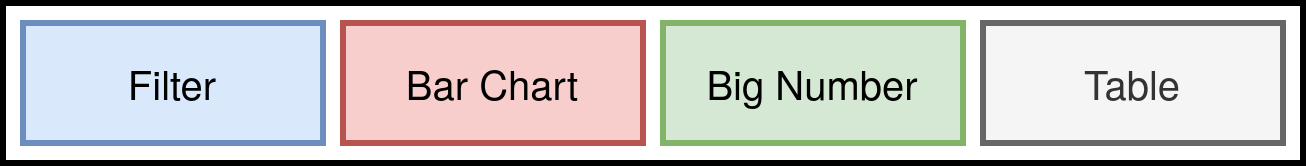
\includegraphics[width=1\linewidth]{images/dashboardsLayout} \caption{Example of a dashboards tool presenting the databases available in the network (simulated data)}\label{fig:dashboardsLayout}
\end{figure}

\hypertarget{license}{%
\subsection*{License}\label{license}}
\addcontentsline{toc}{subsection}{License}

The system is open-source
and this manual was written in \href{https://rmarkdown.rstudio.com}{RMarkdown} using the \href{https://bookdown.org}{bookdown} package.

\hypertarget{acknowledges}{%
\subsection*{Acknowledges}\label{acknowledges}}
\addcontentsline{toc}{subsection}{Acknowledges}

This work has been conducted in the context of EHDEN, a project that receives funding from the European Union's Horizon 2020 and EFPIA through IMI2 Joint Undertaking initiative, under grant agreement No 806968.

\hypertarget{introduction}{%
\chapter{Introduction}\label{introduction}}

The OHDSI research network has been growing steadily which results in an increasing number of healthcare databases standardized to the OMOP CDM format. The OHDSI community created the ACHILLES tool (Automated Characterization of Health Information at Large-scale Longitudinal Exploration System) to characterize those databases. The results are available to the data custodian in their local ATLAS tool and helps them to gain insights in their data and helps in assessing the feasibility of a particular research questions.

ACHILLES was designed to extract the metadata from a single database, which by itself does not allow the comparison with the remaining databases in the network. However, we believe there is even more value in sharing this information with others to enable network research in a Data Network Dashboard.

Data Network Dashboard

The European Health Data and Evidence Network (EHDEN) project therefore designed a Data Network Dashboard tool, a web application to aggregate information from distributed OMOP CDM databases. It uses the ACHILLES results files to construct graphical dashboards and enables database comparison (Figure \ref{fig:intro}). The tool is built on Apache Superset, which is an open-source enterprise-ready business intelligence web application that can provide powerful and fully customizable graphical representations of data. Achilles results can be uploaded through the EHDEN Database Catalogue using the dashboards plugin but can also be directly uploaded in the tool. Figure 1. Example of a dashboards tool presenting age and gender distributions (simulated data).

\begin{figure}
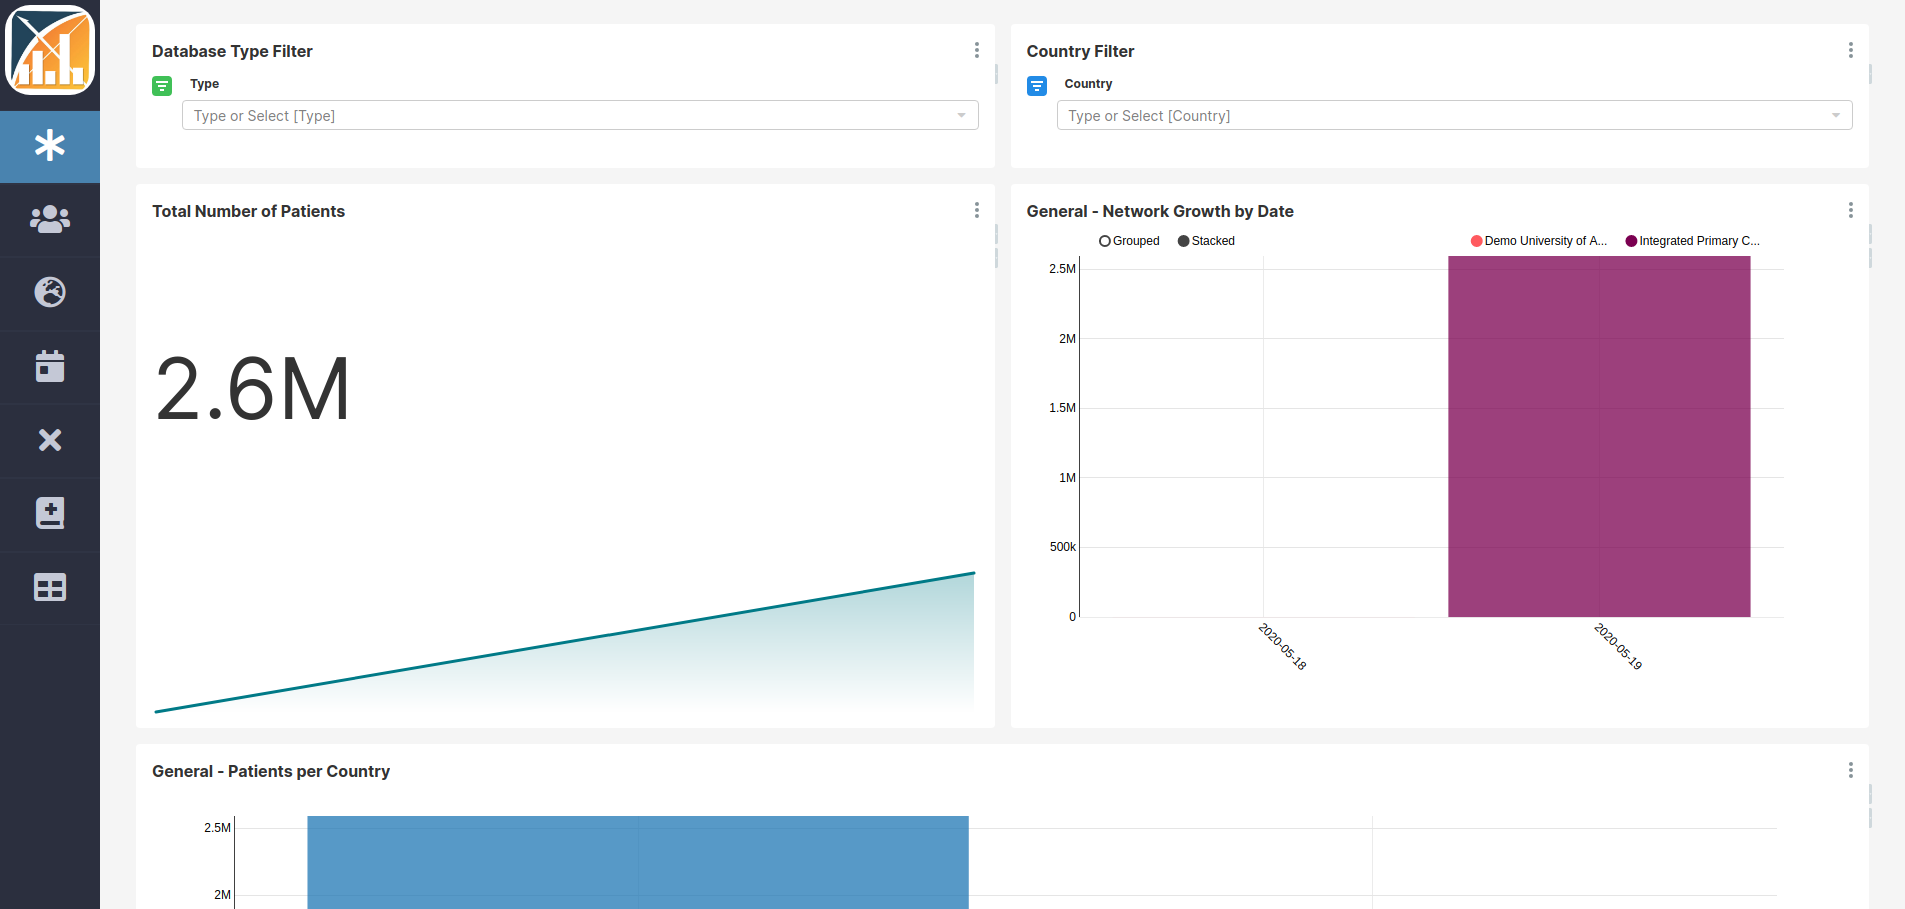
\includegraphics[width=1\linewidth]{images/01-intro} \caption{Example of a dashboards tool presenting the databases available in the network (simulated data)}\label{fig:intro}
\end{figure}

In this tools, we defined and implemented a series of charts and dashboards containing the most relevant information about the databases, such as:

\begin{itemize}
\tightlist
\item
  \textbf{General}: dashboards that shows the databases types per country, the distribution of data source types, the growth of the Network including the number of database and the number of patients in the databases over time;
\item
  \textbf{Person}: representing the number of patients per country, age distribution at first observation, year of birth distribution and normalized gender distribution;
\item
  \textbf{Population characteristics}: dashboard with the cumulative patient time, persons with continuous observation per month, and the start and end dates of those periods;
\item
  \textbf{Visit}: chart to compare the number and type of visit occurrence records;
\item
  \textbf{Death}: information about the number of death records by month, and the patient age at time of death;
\item
  \textbf{Concepts}: bubble chart which shows the number of patients and records per concept over the databases;
\item
  \textbf{Data domains}: heat map visualization of the major data domains in each database.
\end{itemize}

\hypertarget{installation}{%
\chapter{Installation}\label{installation}}

Currently, we use docker to deploy our environment

\hypertarget{first-steps}{%
\subsection*{First Steps}\label{first-steps}}
\addcontentsline{toc}{subsection}{First Steps}

\begin{enumerate}
\def\labelenumi{\arabic{enumi}.}
\item
  Clone the repository with the command \texttt{git\ clone\ -\/-recurse-submodules\ https://github.com/EHDEN/NetworkDashboards}. If you already cloned the repository without the \texttt{-\/-recurse-submodules} option, run \texttt{git\ submodule\ update\ -\/-init} to fetch the superset submodule.
\item
  Create a \texttt{.env} file on the \texttt{docker} directory, using \texttt{.env-example} as a reference, setting all necessary environment variables (\texttt{SUPERSET\_MAPBOX\_API\_KEY} and \texttt{DASHBOARD\_VIEWER\_SECRET\_KEY}).

  2.1 If you will use this application as a third-party application and will iframe it, set the variable \texttt{SINGLE\_APPLICATION\_MODE} to \texttt{False} and define the host of the main application on the variable \texttt{MAIN\_APPLICATION\_HOST}. Also make sure to add this last host to the list of \texttt{ALLOWED\_HOSTS}.
\end{enumerate}

\hypertarget{dashboard-viewer-setup}{%
\subsection*{Dashboard Viewer setup}\label{dashboard-viewer-setup}}
\addcontentsline{toc}{subsection}{Dashboard Viewer setup}

\begin{enumerate}
\def\labelenumi{\arabic{enumi}.}
\item
  If you wish to expose the dashboard viewer app through a specific domain(s) you must add it/them to the \texttt{ALLOWED\_HOSTS} list on file \texttt{dashboard\_viewer/dashboard\_viewer/settings.py} and remove the \texttt{\textquotesingle{}*\textquotesingle{}} entry.
\item
  Build containers' images: \texttt{docker-compose\ build}. This might take several minutes.
\item
  Set up the database and create an admin account for the dashboard viewer app: \texttt{docker-compose\ run\ -\/-rm\ dashboard\ ./docker-init.sh}.
\end{enumerate}

\hypertarget{insert-concepts}{%
\subsection*{Insert Concepts}\label{insert-concepts}}
\addcontentsline{toc}{subsection}{Insert Concepts}

The concepts table is not in the repository due to its dimension, therefore we use directly the Postgres console to insert this table in the installation.

\begin{enumerate}
\def\labelenumi{\arabic{enumi}.}
\item
  Get your concept csv file from \href{https://athena.ohdsi.org/}{Athena}
\item
  Copy the file into postgres container

\begin{Shaded}
\begin{Highlighting}[]
\ExtensionTok{docker}\NormalTok{ cp concept.csv dashboard\_viewer\_postgres\_1:/tmp/}
\end{Highlighting}
\end{Shaded}
\item
  Enter in the postgres container:

\begin{Shaded}
\begin{Highlighting}[]
\ExtensionTok{docker}\NormalTok{ exec {-}it dashboard\_viewer\_postgres\_1 bash}
\end{Highlighting}
\end{Shaded}
\item
  Enter in the \texttt{achilles} database (value of the variable \texttt{POSTGRES\_ACHILLES\_DB} on the .env file) with the \texttt{root} user (value of the variable \texttt{POSTGRES\_ROOT\_USER} on the .env file):

\begin{verbatim}
psql achilles root
\end{verbatim}
\item
  Create the \texttt{concept} table

\begin{Shaded}
\begin{Highlighting}[]
\KeywordTok{CREATE} \KeywordTok{TABLE}\NormalTok{ concept (}
\NormalTok{  concept\_id         }\DataTypeTok{INTEGER}        \KeywordTok{NOT} \KeywordTok{NULL}\NormalTok{,}
\NormalTok{  concept\_name       }\DataTypeTok{VARCHAR}\NormalTok{(}\DecValTok{255}\NormalTok{)   }\KeywordTok{NOT} \KeywordTok{NULL}\NormalTok{,}
\NormalTok{  domain\_id          }\DataTypeTok{VARCHAR}\NormalTok{(}\DecValTok{20}\NormalTok{)    }\KeywordTok{NOT} \KeywordTok{NULL}\NormalTok{,}
\NormalTok{  vocabulary\_id      }\DataTypeTok{VARCHAR}\NormalTok{(}\DecValTok{20}\NormalTok{)    }\KeywordTok{NOT} \KeywordTok{NULL}\NormalTok{,}
\NormalTok{  concept\_class\_id   }\DataTypeTok{VARCHAR}\NormalTok{(}\DecValTok{20}\NormalTok{)    }\KeywordTok{NOT} \KeywordTok{NULL}\NormalTok{,}
\NormalTok{  standard\_concept   }\DataTypeTok{VARCHAR}\NormalTok{(}\DecValTok{1}\NormalTok{)     }\KeywordTok{NULL}\NormalTok{,}
\NormalTok{  concept\_code       }\DataTypeTok{VARCHAR}\NormalTok{(}\DecValTok{50}\NormalTok{)    }\KeywordTok{NOT} \KeywordTok{NULL}\NormalTok{,}
\NormalTok{  valid\_start\_date   }\DataTypeTok{DATE}           \KeywordTok{NOT} \KeywordTok{NULL}\NormalTok{,}
\NormalTok{  valid\_end\_date     }\DataTypeTok{DATE}           \KeywordTok{NOT} \KeywordTok{NULL}\NormalTok{,}
\NormalTok{  invalid\_reason     }\DataTypeTok{VARCHAR}\NormalTok{(}\DecValTok{1}\NormalTok{)     }\KeywordTok{NULL}
\NormalTok{);}
\end{Highlighting}
\end{Shaded}
\item
  Copy the CSV file content to the table (this could take a while)

  To get both \texttt{\textquotesingle{}} (single quotes) and \texttt{"} (double quotes) on the \texttt{concept\_name} column we use a workaround by setting the quote character to one that should never be in the text. Here we used \texttt{\textbackslash{}b} (backslash).

\begin{Shaded}
\begin{Highlighting}[]
\KeywordTok{COPY} \KeywordTok{public}\NormalTok{.concept }\KeywordTok{FROM} \StringTok{\textquotesingle{}/tmp/concept.csv\textquotesingle{}} \KeywordTok{WITH}\NormalTok{ CSV }\KeywordTok{HEADER}
\NormalTok{  DELIMITER E}\StringTok{\textquotesingle{}}\CharTok{\textbackslash{}t}\StringTok{\textquotesingle{}}\NormalTok{ QUOTE E}\StringTok{\textquotesingle{}}\CharTok{\textbackslash{}b}\StringTok{\textquotesingle{}}\NormalTok{;}
\end{Highlighting}
\end{Shaded}
\item
  Create index in table (this could take a while):

\begin{Shaded}
\begin{Highlighting}[]
\KeywordTok{CREATE} \KeywordTok{INDEX}\NormalTok{ concept\_concept\_id\_index }\KeywordTok{ON}\NormalTok{ concept (concept\_id);}
\KeywordTok{CREATE} \KeywordTok{INDEX}\NormalTok{ concept\_concept\_name\_index }\KeywordTok{ON}\NormalTok{ concept (concept\_name);}
\end{Highlighting}
\end{Shaded}
\item
  Set the owner of the \texttt{concept} table to the \texttt{achilles} user (value of the variable \texttt{POSTGRES\_ACHILLES\_USER} on the .env file):

\begin{verbatim}
ALTER TABLE concept OWNER TO achiller
\end{verbatim}
\item
  Bring up the containers: \texttt{docker-compose\ up\ -d}.
\item
  Run the command \texttt{docker-compose\ run\ -\/-rm\ dashboard\ python\ manage.py\ generate\_materialized\_views} to create the materialized views on Postgres.
\end{enumerate}

\hypertarget{superset-setup}{%
\subsection*{Superset setup}\label{superset-setup}}
\addcontentsline{toc}{subsection}{Superset setup}

\begin{enumerate}
\def\labelenumi{\arabic{enumi}.}
\item
  Bring up the containers: \texttt{docker-compose\ up\ -d}.
\item
  Make sure that the container \texttt{superset-init} has finished before continuing. It is creating the necessary tables on the database and creating permissions and roles.
\item
  If you used the default ports:

  \begin{itemize}
  \tightlist
  \item
    Go to \texttt{http://localhost} to access the dashboard viewer app.
  \item
    Go to \texttt{http://localhost:8088} to access superset.
  \end{itemize}
\item
  By default Superset's admin user credentials are admin/admin.
  It is recommended that you change the password if you will use this in a production environment.
\item
  To any anonymous user view dashboards, add the following permissions to the public role:

  \begin{itemize}
  \tightlist
  \item
    all datasource access on all\_datasource\_access
  \item
    can csrf token on Superset
  \item
    can dashboard on Superset
  \item
    can explore json on Superset
  \item
    can read on Chart
  \item
    can read on CssTemplate
  \item
    can read on Dashboard
  \end{itemize}
\item
  For each dashboard you want anonymous users to be able to access, on the dashboard list page click edit (the pencil on the right) and add the ``Admin'' and ``Public'' roles to the ``Roles with acess'' field.
\end{enumerate}

\hypertarget{dummy-data}{%
\subsection*{Dummy data}\label{dummy-data}}
\addcontentsline{toc}{subsection}{Dummy data}

On a fresh installation, there are no achilles\_results data so Superset's dashboards will display ``No results''. On the root of this repository, you can find the \texttt{demo} directory where we have an ACHILLES results file with synthetic data that you can upload to a data source on the uploader app of the dashboard viewer (\url{http://localhost/uploader}). If you wish to compare multiple data sources, on the \texttt{demo} directory there is also a python script that allows you to generate new ACHILLES results files, where it generates random count values based on the ranges of values for each set of analysis\_id and stratums present on a base ACHILLES results file. So, from the one ACHILLES results fill we provided, you can have multiple data sources with different data.

\hypertarget{processes}{%
\chapter{Processes}\label{processes}}

\hypertarget{data-sources}{%
\subsection*{Data Sources}\label{data-sources}}
\addcontentsline{toc}{subsection}{Data Sources}

\textbf{Target: platform user}

Before uploading any data to this platform, a data source owner has to create a data source instance to then associated the upload data with.

The creation of data source is done through the \texttt{{[}BASE\_URL{]}/uploader/} URL, where 7 fields are expected:

\begin{enumerate}
\def\labelenumi{\arabic{enumi}.}
\tightlist
\item
  name: an extensive name
\item
  acronym: a short name
\item
  country: where is the data source localized
\item
  link (Optional): web page of the data source
\item
  database type: type of OMOP database
\item
  coordinates: a more accurate representation of the data source's localization
\item
  hash (Optional): the internal unique identifier of a data source
\end{enumerate}

If you access \texttt{{[}BASE\_URL{]}/uploader/} the 7th field (hash) is set automatically for something random, however, if you want to set it use the \texttt{{[}BASE\_URL{]}/uploader/{[}HASH{]}/} URL.

To avoid duplication on the database type field, this field is transformed (use title case and trimmed) and then is checked there is already a record (Database Type) with the same value.

There are several ways to create a data source:

\begin{enumerate}
\def\labelenumi{\arabic{enumi}.}
\tightlist
\item
  Create through a web form
\end{enumerate}

By accessing the \texttt{{[}BASE\_URL{]}/uploader/} URL, you will get a form where you can field the fields, where the country field is a dropdown and the coordinates field is set through a map widget.

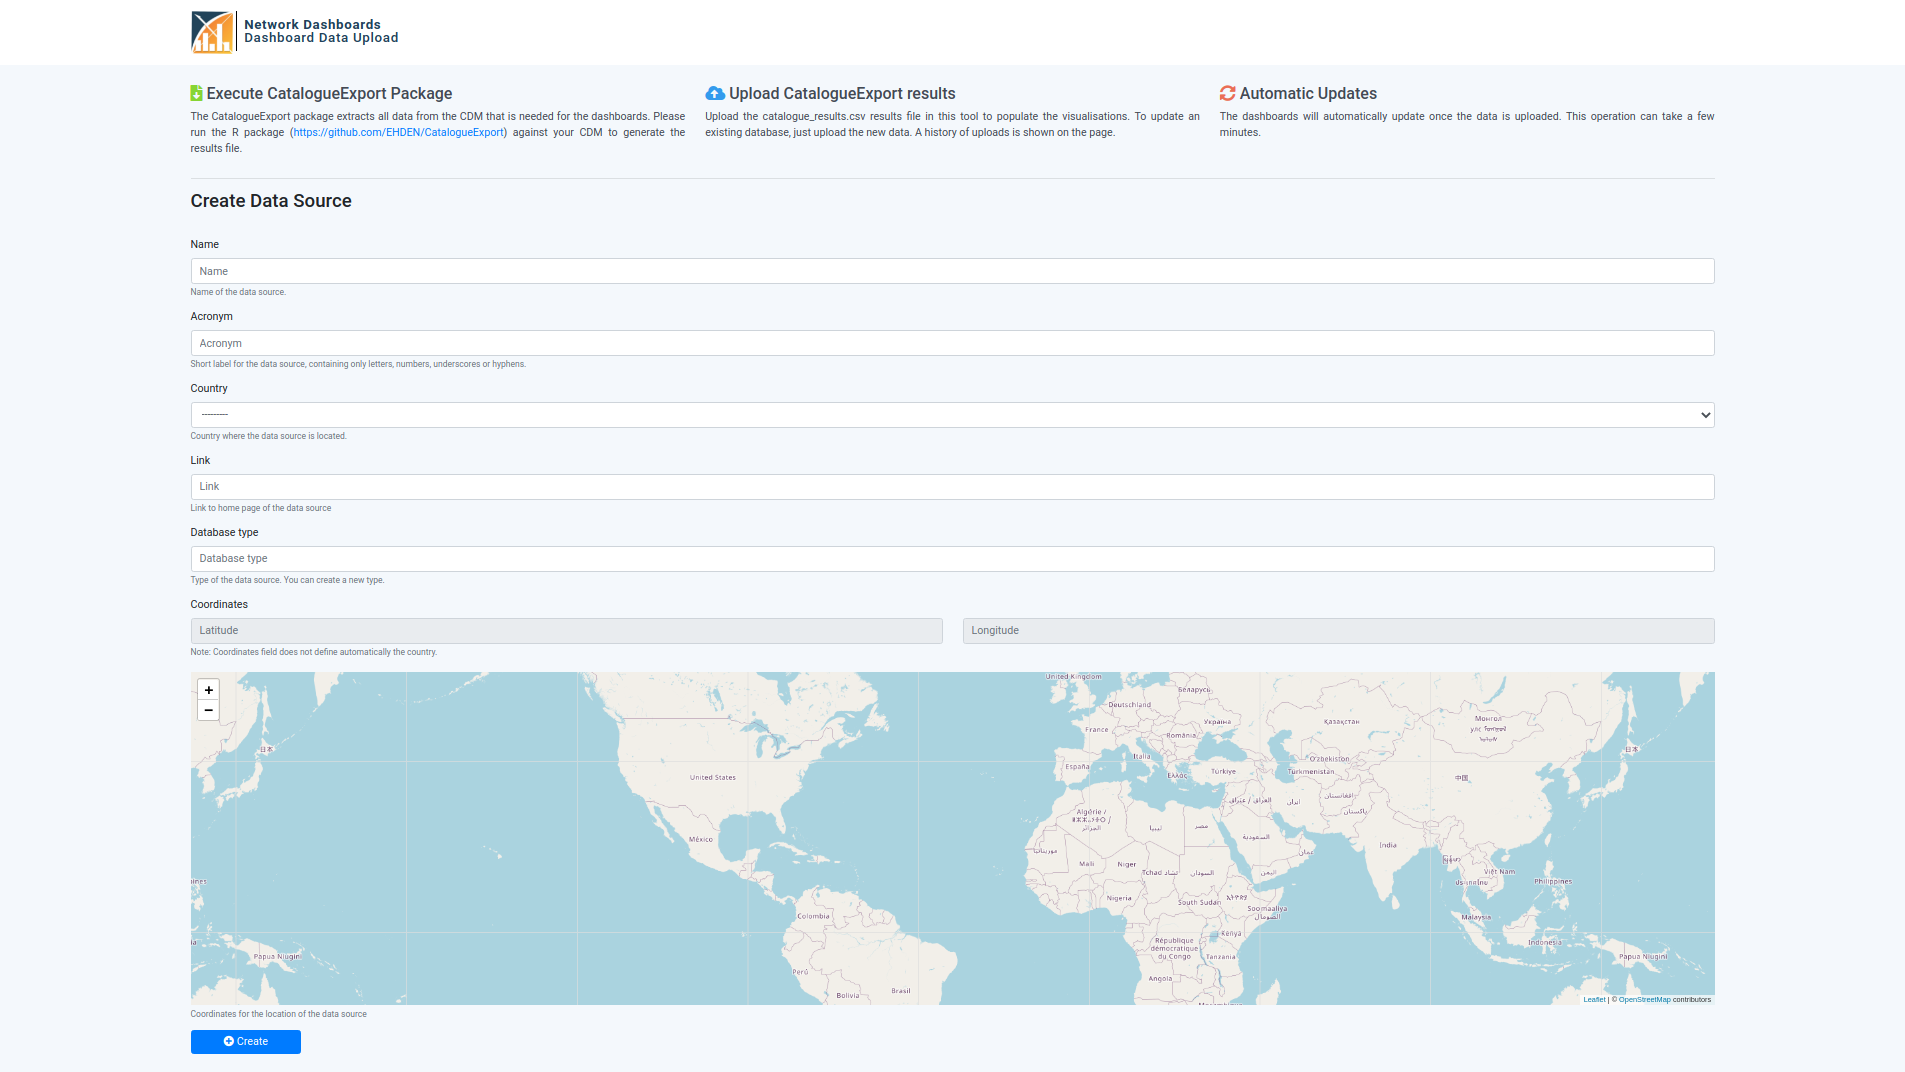
\includegraphics{images/processes/processes_data_source_creation.png}

\begin{enumerate}
\def\labelenumi{\arabic{enumi}.}
\setcounter{enumi}{1}
\tightlist
\item
  Automatically create when performing a GET to the \texttt{{[}BASE\_URL{]}/uploader/} URL
\end{enumerate}

If the Network Dashboards platform is being used as a third-party application and the main application has all the data for the required fields, the data source can be automatically created and the user is redirected directly to the upload files page.

To perform this, each field should be provided as a URL parameter when accessing the \texttt{{[}BASE\_URL{]}/uploader/} URL. If all required fields are provided and are valid the data source is created and the user is redirected to the upload files page. If a required field is missing or is not valid the webform is presented to the user so it can manually fill those fields.

\begin{enumerate}
\def\labelenumi{\arabic{enumi}.}
\setcounter{enumi}{2}
\tightlist
\item
  Automatically create by performing a POST to the \texttt{{[}BASE\_URL{]}/uploader/} URL
\end{enumerate}

Since the creation URL does not have csrf cookie protection, you can perform a POST request as you were submitting a form.

\textbf{Notes For the automatic options}:

\begin{itemize}
\item
  Since the coordinates field is composed of two fields (latitude, longitude), it should be submitted as \texttt{coordinates\_0={[}latitude{]}} and \texttt{coordinates\_1={[}longitude{]}}
\item
  The country field should match one of the available on the dropdown of the webform.
\end{itemize}

\hypertarget{draft-status}{%
\subsubsection*{Draft Status}\label{draft-status}}
\addcontentsline{toc}{subsubsection}{Draft Status}

After a data owner uploads data into his data source, he might not want to make it public right away.
To achieve this a data source has a boolean field telling whether if the data source is in draft mode.
This then also allows creating dashboards with data of non-draft data sources only.

There are three ways to change the value of this draft status field:

\begin{enumerate}
\def\labelenumi{\arabic{enumi}.}
\tightlist
\item
  Through the Django admin app (\texttt{{[}BASE\_URL{]}/admin/})
\item
  Accessing the respective edit page of the data source. This requires a feature to be enabled, which is more detailed on the \href{customizations.html\#allow-draft-status-updates}{Allow Draft Status Updates} section of the Customization chapter.
\item
  Perform a PATCH request to the \texttt{{[}BASE\_URL{]}/uploader/{[}HASH{]}/} URL. On this request, other fields, other than the draft status, can be changed. The body of the request must be a JSON object with the fields that will suffer changes and their new values.
\end{enumerate}

\hypertarget{catalogue-results-files}{%
\subsection*{Catalogue Results Files}\label{catalogue-results-files}}
\addcontentsline{toc}{subsection}{Catalogue Results Files}

\textbf{Target: platform user}

Once a data source is created you can access its upload page by accessing the \texttt{{[}BASE\_URL{]}/uploader/{[}HASH{]}/}. If no data source has the provided hash you will be redirected back to the data source creation form.

On the upload page you can:

\begin{enumerate}
\def\labelenumi{\arabic{enumi}.}
\tightlist
\item
  Go to the edit page of your data source
\item
  Upload a catalogue results file
\item
  Check the upload history
\end{enumerate}

A catalogue results file is a CSV file, the result obtained after running the \href{https://github.com/EHDEN/CatalogueExport}{EHDEN/CatalogueExport} R package on an OMOP database. It is a variant of the \href{https://github.com/OHDSI/Achilles}{OHDSI/Achilles} where it only extracts a subset of analyses of the ACHILLES' original set.

The upload form expects a CSV file with the following columns:

\begin{longtable}[]{@{}lll@{}}
\toprule
Name & Type & Required/Non-Nullable/Non-Empty\tabularnewline
\midrule
\endhead
analysis\_id & int & Yes\tabularnewline
stratum\_1 & string & No\tabularnewline
stratum\_2 & string & No\tabularnewline
stratum\_3 & string & No\tabularnewline
stratum\_4 & string & No\tabularnewline
stratum\_5 & string & No\tabularnewline
count\_value & int & Yes\tabularnewline
min\_value & double & No\tabularnewline
max\_value & double & No\tabularnewline
avg\_value & double & No\tabularnewline
stdev\_value & double & No\tabularnewline
median\_value & double & No\tabularnewline
p10\_value & double & No\tabularnewline
p25\_value & double & No\tabularnewline
p75\_value & double & No\tabularnewline
p90\_value & double & No\tabularnewline
\bottomrule
\end{longtable}

The uploaded file must:

\begin{itemize}
\item
  either contain the first 7 columns OR all 16 columns
\item
  contain the columns in the same order as presented in the table above
\end{itemize}

While parsing the uploaded file, some data is extracted to then present on the Upload history and to update data source information. This data is extracted from the record with analysis id 0, \textbf{which is required to be present on the file}, and 5000, which is optional. Next is presented the data extracted and their description:

\begin{itemize}
\item
  R Package Version: the version of CatalogueExport R package used
\item
  Generation Date: date at which the CatalogueExport was executed on the OMOP database
\item
  Source Release Date: date at which the OMOP database was released
\item
  CDM Release Date: date at which the used CDM version was released
\item
  CDM Version: version of the CDM used
\item
  Vocabulary Version: version of the vocabulary used
\end{itemize}

The next table is presented where the previous data is stored on the rows with analysis id 0 and 5000:

\begin{longtable}[]{@{}rlllll@{}}
\toprule
Analysis Id & Stratum 1 & Stratum 2 & Stratum 3 & Stratum 4 & Stratum 5\tabularnewline
\midrule
\endhead
0 & & R Package Version & Generation Date & &\tabularnewline
5000 & & Source Release Date & CDM Release Date & CDM Version & Vocabulary Version\tabularnewline
\bottomrule
\end{longtable}

\hypertarget{materialized-views}{%
\subsection*{Materialized Views}\label{materialized-views}}
\addcontentsline{toc}{subsection}{Materialized Views}

\textbf{Target: admin user}

For each chart, Superset has an underlying SQL query which in our case is run every time a chart is rendered. If one of these queries takes too long to execute the charts will also take too long until they are rendered and eventually users might get timeout messages given a bad user experience.

To avoid this problem, instead of executing the raw SQL query we create a \href{https://www.postgresql.org/docs/10/rules-materializedviews.html}{postgres materialized view} of the query, which is then used to feed the data to the chart. So only a simple \texttt{SELECT\ x\ FROM\ x} query is executed when a chart is rendered.

So whenever I create a chart I have to access the Postgres console? No, we created an unmanaged Materialized Queries model that maps to the materialized views on Postgres. With it you can create new materialized views through the Django admin app, by accessing the \texttt{{[}BASE\_URL{]}/admin/} URL.

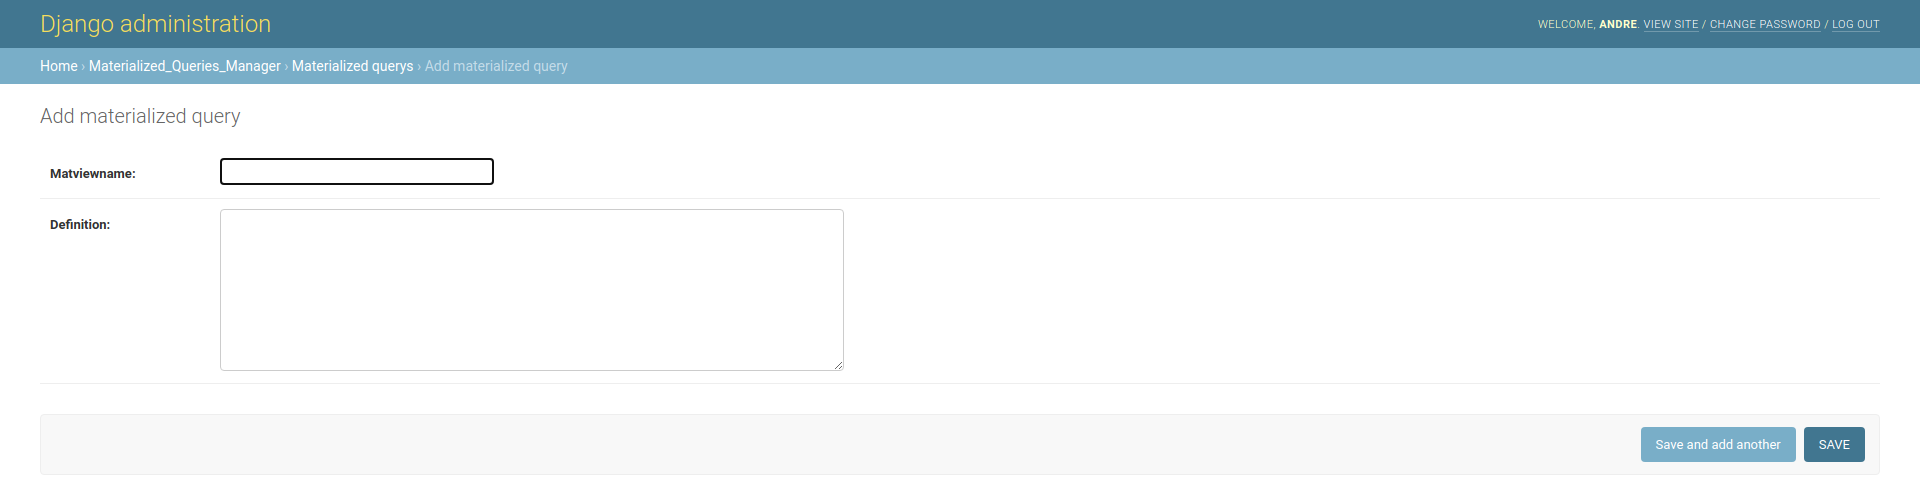
\includegraphics{images/processes/processes_materialized_view_creation.png}

You have to provide the materialized view name and its query, which will then be used to execute the query \texttt{CREATE\ MATERIALIZED\ VIEW\ {[}name{]}\ AS\ {[}query{]}}, which will be executed on a background task so the browser doesn't hang and times out, in case of complicated queries. Taking this into account, the record associated will not appear on the Django admin app until the \texttt{CREATE\ MATERIALIZED\ VIEW} query finishes.

To give feedback on the background task we use \href{https://github.com/celery/django-celery-results}{celery/django-celery-results}, so you can check the status of a task on the Task Results model of the Celery Results app

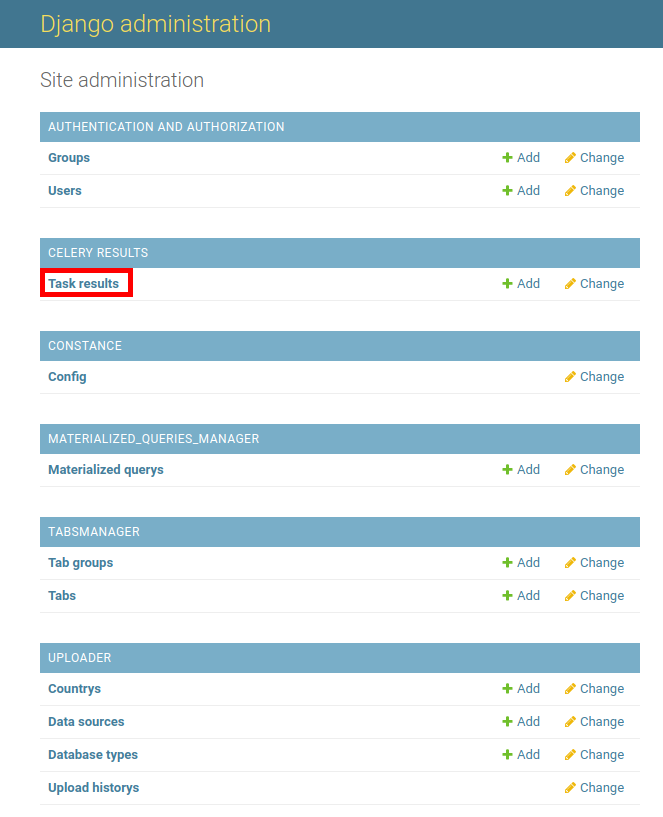
\includegraphics{images/processes/processes_task_results.png}

After the creation of a Materialized Query, the will be a message telling the id of the task which is executing the \texttt{CREATE\ MATERIALIZED\ VIEW} query. You can then check for the record associated with the task, click on the id to get more details. If something went wrong check the error message either on Result Data or Traceback fields under the Result section

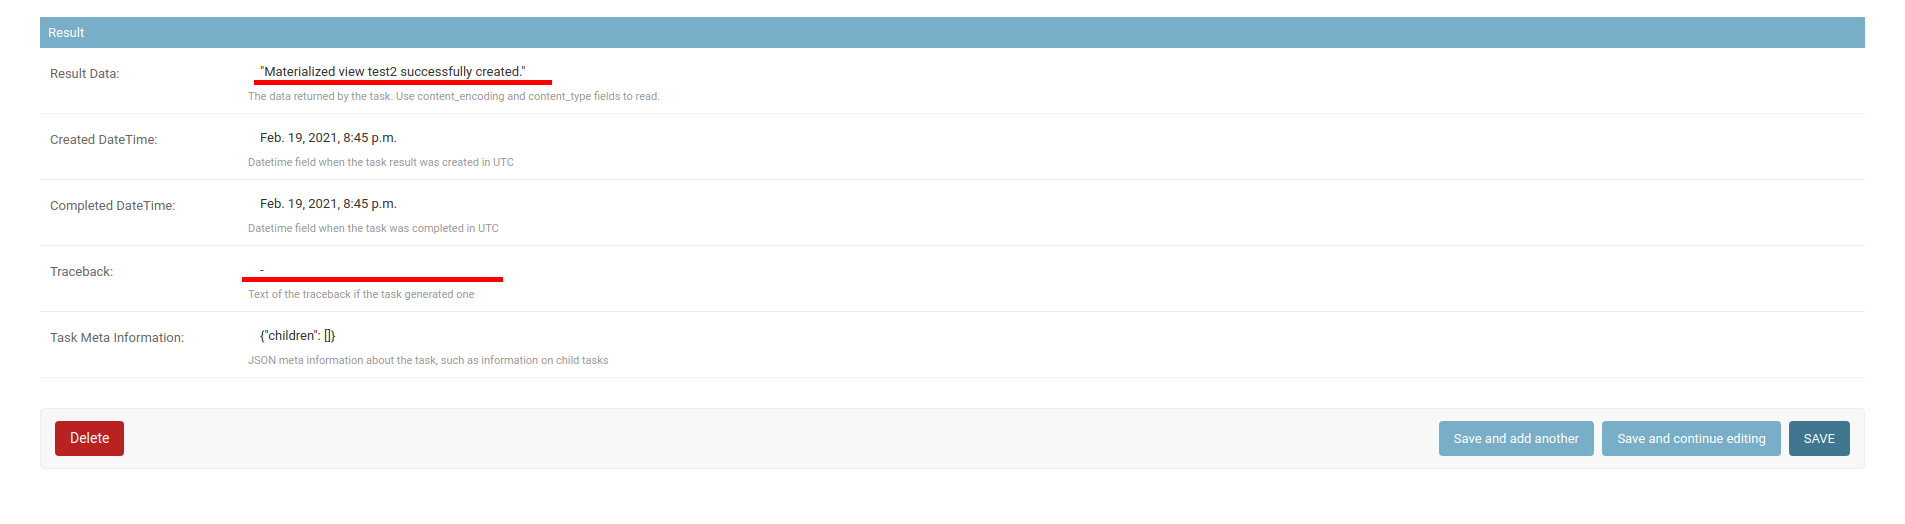
\includegraphics{images/processes/processes_task_result_info.png}

After all this, the final step is to add the materialized view as a Dataset. Login into Superset, then go to Data -\textgreater{} Datasets and create a new one. Select the \texttt{Achilles} database, the \texttt{public} schema, then the created materialized view and click ``ADD''. After this, the materialized view can be used as a data source for a new chart.

\hypertarget{tabs-view-deprecated}{%
\subsection*{Tabs View {[}Deprecated{]}}\label{tabs-view-deprecated}}
\addcontentsline{toc}{subsection}{Tabs View {[}Deprecated{]}}

Note: This app is no longer maintaned and the associated urls were unlinked.

\textbf{Target: admin user}

Once there are data sources on the platform, data was uploaded to them and there are dashboards created on Superset, researchers can now browse through the dashboards and analyze and compare the data of the different data sources.
One way to allow this would be to let them browse through the dashboard list on Superset. However, if there was some dashboards not ready to show to the public users, they could still access them.

For that, it was created a page, with a sidebar, where public users could browse through the available and ready dashboards.
It can be accessed through the URL \texttt{{[}BASE\_URL{]}/tabs/}

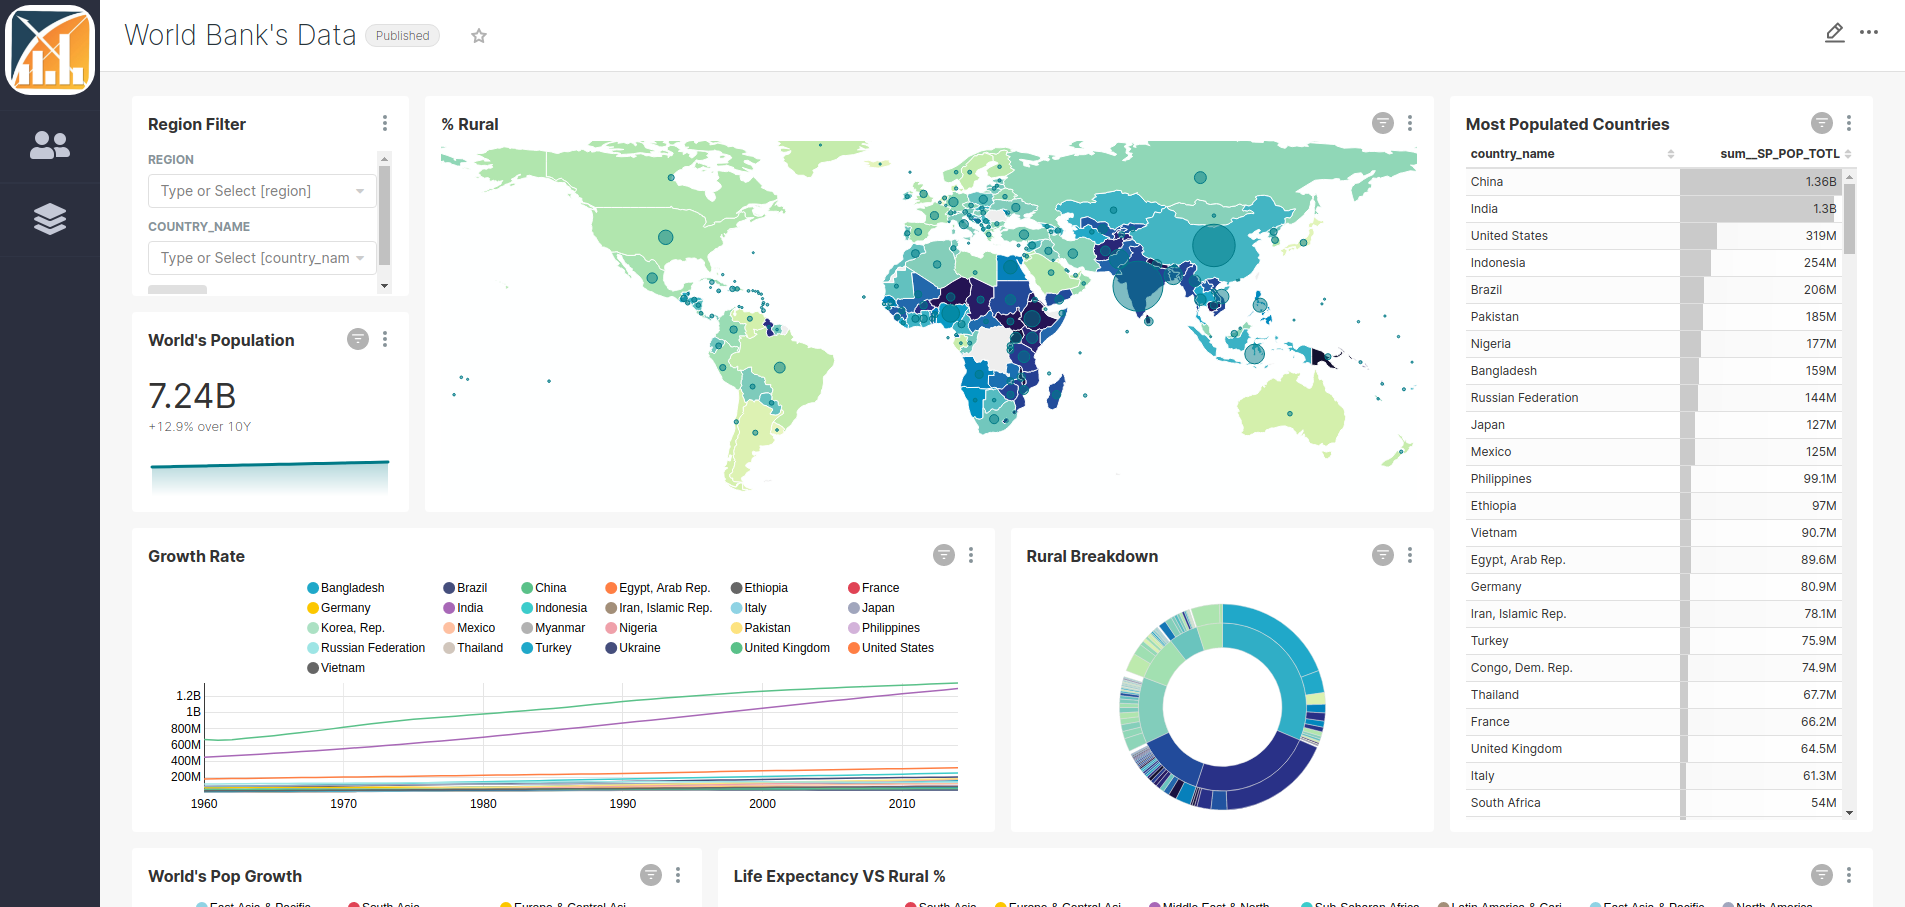
\includegraphics{images/processes/tabs.png}

The sidebar entries can be configured through the Django admin app, accessing the Tabsmanager app section.
Here two models are available to create:

\begin{itemize}
\tightlist
\item
  Tab Groups: They allow to groups several sidebar entries within a collapsable group.
\end{itemize}

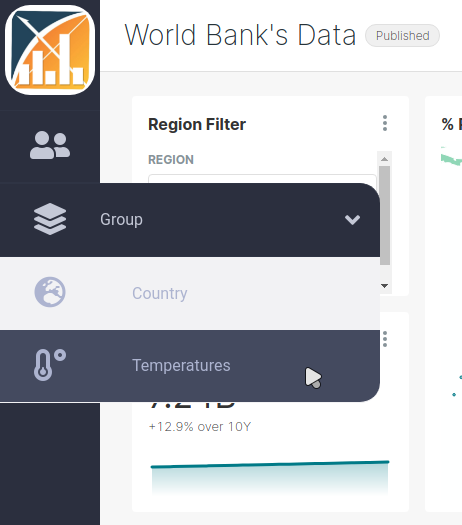
\includegraphics{images/processes/tabs-group.png}

\begin{itemize}
\tightlist
\item
  Tabs: Will create a clickable entry on the sidebar that can be presented within a group. When a tab is clicked the associated dashboard will be displayed on the page.
\end{itemize}

Each entry, tab, or group of them, expects:

\begin{itemize}
\tightlist
\item
  Title/Name
\item
  Icon: Name of a font awesome version 5 icon
\item
  Position: Allows to order entries along the sidebar. If a Tab has a group, then this field will order the tabs within that group only.
\item
  Visible: If whether or not this tab or group should be visible. The goal of this field is to avoid having to delete the record from the database just because a certain tab is not ready and later on created it from scratch.
\end{itemize}

Tabs additionally expect an URL, which will be used to display a Superset dashboard in an iframe.
To hide Superset's menu bar, an additional \texttt{standalone} URL parameter should be appended to the provided URL of a tab.
The value of the \texttt{standalone} arguments depends on the expected result:

\begin{itemize}
\tightlist
\item
  1: menu bar is hidden. the bar where the dashboard title, publish status, and three dots option menu are present will still appear
\item
  2: both the menu bar and the dashboard title bar are hidden.
\end{itemize}

By default, the dashboard of the first tab is displayed on the page, however, if one wants a specific tab to be displayed when the page is opened, its title should be present in the hash part of the URL.
For example, if there is a tab called People, to make that tab selected at the start the following URL should be used \texttt{{[}BASE\_URL{]}/tabs/\#People}.

\hypertarget{backups}{%
\chapter{Backups}\label{backups}}

\begin{enumerate}
\def\labelenumi{\arabic{enumi}.}
\item
  Create a credentials file (the structure of the file depends on the target cloud server)
\item
  Create a \texttt{backups.conf} under the \texttt{backups} directory using \texttt{backups.conf.example} as base, setting the appropriate value for the several variables.

  For variables associated with files and directories always use \emph{absolute} paths.

  Variables:

  \begin{itemize}
  \item
    \texttt{RUN}: Set it to \texttt{0} if you don't want the next scheduled backup to run.

    This variable allows you to cancel any backup runs while you are doing some maintenance on the application.
  \item
    \texttt{CONSTANCE\_REDIS\_DB}: Number of the Redis database where the django constance config is stored. The default value is 2. This value should be the same as the environment variable \texttt{REDIS\_CONSTANCE\_DB} of the dashboard container.
  \item
    The following variables are associated with the arguemtns of the \texttt{backup\_uploader} python package. Check its \href{https://github.com/aspedrosa/BackupUploader\#usage}{usage} for more details:

    \begin{itemize}
    \item
      \texttt{APP\_NAME}: The backup process will generate some directories with this name in places that are shared with other applications.
    \item
      \texttt{SERVER}: The name of the target cloud server to where backups should be uploaded (dropbox or mega).
    \item
      \texttt{BACKUP\_CHAIN\_CONFIG}: Allows having different directories with backups of different ages.
    \item
      \texttt{CREDENTIALS\_FILE\_PATH}: File containing the credentials to access the server to upload the backup file.
    \end{itemize}
  \end{itemize}
\item
  Install the \texttt{backup\_uploader} python package by following its \href{https://github.com/aspedrosa/BackupUploader\#install}{install} instructions.
\item
  Schedule your backups

\begin{Shaded}
\begin{Highlighting}[]
\ExtensionTok{*}\NormalTok{    *    *   *    *  Command\_to\_execute}
\KeywordTok{|}    \KeywordTok{|}    \KeywordTok{|}    \KeywordTok{|}   \KeywordTok{|}       
\KeywordTok{|}    \KeywordTok{|}    \KeywordTok{|}    \KeywordTok{|}    \ExtensionTok{Day}\NormalTok{ of the Week ( 0 {-} 6 ) }\KeywordTok{(} \ExtensionTok{Sunday}\NormalTok{ = 0 }\KeywordTok{)}
\KeywordTok{|}    \KeywordTok{|}    \KeywordTok{|}    \KeywordTok{|}
\KeywordTok{|}    \KeywordTok{|}    \KeywordTok{|}    \ExtensionTok{Month}\NormalTok{ ( 1 {-} 12 )}
\KeywordTok{|}    \KeywordTok{|}    \KeywordTok{|}
\KeywordTok{|}    \KeywordTok{|}    \ExtensionTok{Day}\NormalTok{ of Month ( 1 {-} 31 )}
\KeywordTok{|}    \KeywordTok{|}
\KeywordTok{|}    \ExtensionTok{Hour}\NormalTok{ ( 0 {-} 23 )}
\KeywordTok{|}
\ExtensionTok{Min}\NormalTok{ ( 0 {-} 59 ) }
\end{Highlighting}
\end{Shaded}

  (Retrived from: \href{https://www.tutorialspoint.com/unix_commands/crontab.htm}{Tutorialspoint})

  Ex: To run every day at 3:00 am

  \begin{enumerate}
  \def\labelenumii{\arabic{enumii}.}
  \item
    \texttt{crontab\ -e}
  \item
    Add entry \texttt{0\ 3\ *\ *\ *\ \$HOME/NetworkDashboards/backups/backup.sh} (The path to the backup script might be different)
  \end{enumerate}
\end{enumerate}

\hypertarget{restore}{%
\subsection*{Restore}\label{restore}}
\addcontentsline{toc}{subsection}{Restore}

\begin{enumerate}
\def\labelenumi{\arabic{enumi}.}
\item
  Select the compressed backup you want to restore.
\item
  Make sure that all the environment variables are the same as the ones that were used for the chosen backup file.
  Additionally, the \texttt{backups.conf} file is also necessary to set up, since the \texttt{TMP\_DIRECTORY} variable will be used.
\item
  Run the \texttt{backups/restore.sh} script.
\end{enumerate}

\hypertarget{useful-stuff}{%
\subsection*{Useful stuff}\label{useful-stuff}}
\addcontentsline{toc}{subsection}{Useful stuff}

\begin{itemize}
\item
  How to create a shared link to a dropbox directory using its python's API:

\begin{Shaded}
\begin{Highlighting}[]
\ExtensionTok{pip}\NormalTok{ install dropbox}
\end{Highlighting}
\end{Shaded}

\begin{Shaded}
\begin{Highlighting}[]
\ImportTok{import}\NormalTok{ dropbox}
\NormalTok{d }\OperatorTok{=}\NormalTok{ dropbox.Dropbox(API\_TOKEN)}

\CommentTok{\# create a shared link for a directory}
\ImportTok{from}\NormalTok{ dropbox.sharing }\ImportTok{import}\NormalTok{ SharedLinkSettings}
\NormalTok{sharing\_settings }\OperatorTok{=}\NormalTok{ SharedLinkSettings(}
\NormalTok{    require\_password}\OperatorTok{=}\VariableTok{True}\NormalTok{,}
\NormalTok{    link\_password}\OperatorTok{=}\NormalTok{DIRECTORY\_PASSWORD,}
\NormalTok{)}
\NormalTok{d.sharing\_create\_shared\_link\_with\_settings(}
\NormalTok{    DIRECTORY\_PATH,}
\NormalTok{    sharing\_settings,}
\NormalTok{)}

\CommentTok{\# get all links}
\ControlFlowTok{for}\NormalTok{ link }\KeywordTok{in}\NormalTok{ d.sharing\_get\_shared\_links().links:}
    \BuiltInTok{print}\NormalTok{(}\SpecialStringTok{f"}\SpecialCharTok{\{}\NormalTok{link}\SpecialCharTok{.}\NormalTok{path}\SpecialCharTok{\}}\SpecialStringTok{ {-}\textgreater{} }\SpecialCharTok{\{}\NormalTok{link}\SpecialCharTok{.}\NormalTok{url}\SpecialCharTok{\}}\SpecialStringTok{"}\NormalTok{)}
\end{Highlighting}
\end{Shaded}
\end{itemize}

\hypertarget{customizations}{%
\chapter{Customizations}\label{customizations}}

This platform is currently being used within the scope of the European Health Data \& Evidence Network (\href{https://www.ehden.eu/}{EHDEN}) project.
To allow the dashboard viewer Django application to be easily used by another project or company, several components support customization in runtime, removing the need to change such things directly on the source code.

To achieve this we make use of \href{https://github.com/jazzband/django-constance}{Constance} that allows configuring several fields which then can be changed through the Django admin app.

\hypertarget{platform-logo}{%
\subsection*{Platform Logo}\label{platform-logo}}
\addcontentsline{toc}{subsection}{Platform Logo}

It is visible both in the Tabs Manager and the Catalogue Results Uploader URLs.

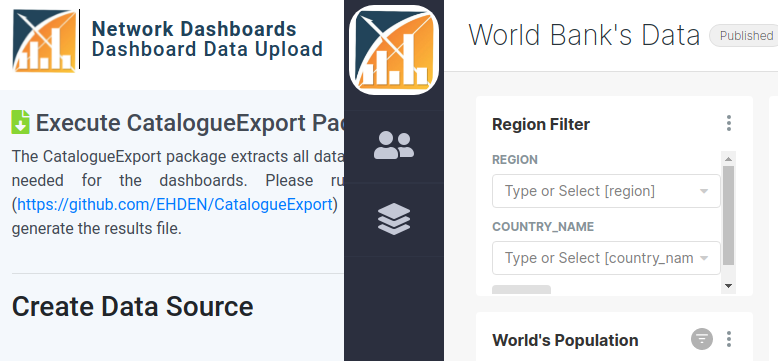
\includegraphics{images/customizations/logo.png}

The platform allows two possible ways to choose a logo: upload a file or provide an URL to an image.

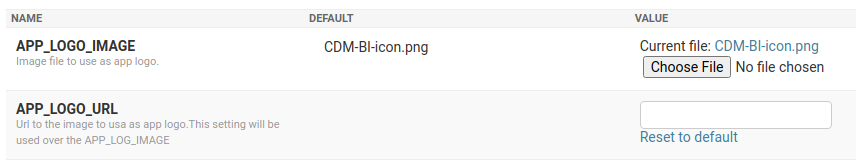
\includegraphics{images/customizations/constance-logo.png}

If both fields are provided, the URL one will be used.

On the tabs manager app, we also allow customization of the CSS associated both with the image itself and its container.

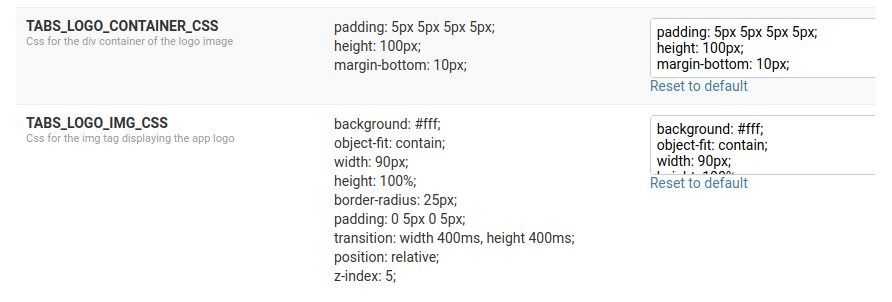
\includegraphics{images/customizations/constance-logo-css.png}

\hypertarget{platform-title}{%
\subsection*{Platform Title}\label{platform-title}}
\addcontentsline{toc}{subsection}{Platform Title}

All pages of the uploader app use the same base HTML file which contains a header with the platform logo, page title, and platform title.


\includegraphics{images/customizations/title.png}

The first was already mentioned before, the second can't be changed.
The last can be altered using a Constance field.


\includegraphics{images/customizations/constance-title.png}

\hypertarget{uploader-page-texts}{%
\subsection*{Uploader Page Texts}\label{uploader-page-texts}}
\addcontentsline{toc}{subsection}{Uploader Page Texts}

The data source creation page has three columns with some text providing some instructions for the creation of a data source and the upload of catalogue results.

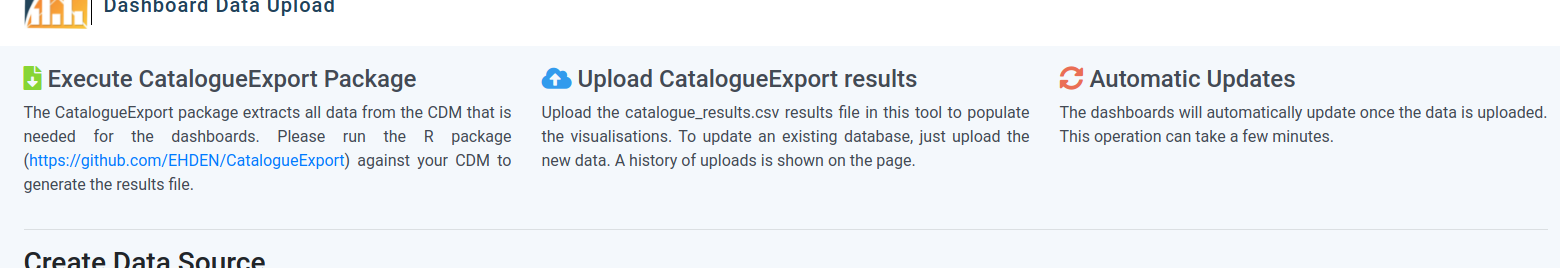
\includegraphics{images/customizations/texts.png}

The text of these three columns is customizable, where \href{https://www.markdownguide.org/}{markdown} can be used, which is then transformed into HTML before rending the page.

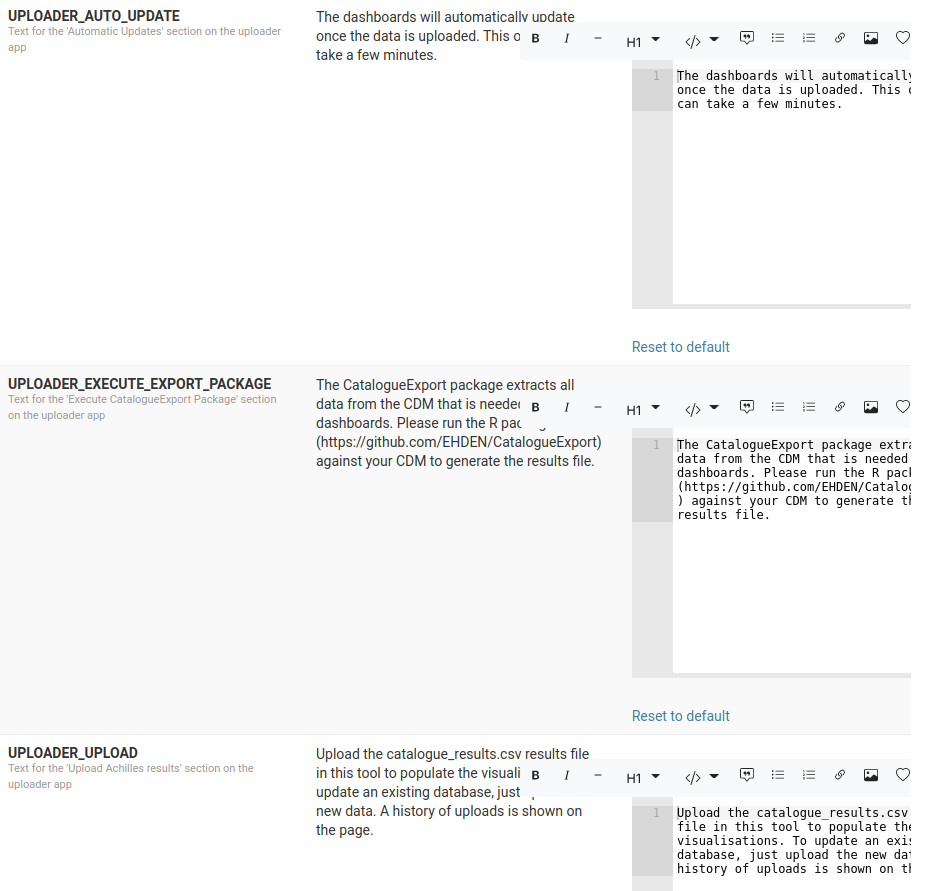
\includegraphics{images/customizations/constance-texts.png}

\hypertarget{allow-draft-status-updates}{%
\subsection*{Allow Draft Status Updates}\label{allow-draft-status-updates}}
\addcontentsline{toc}{subsection}{Allow Draft Status Updates}

In the section \href{processes.html\#draft-status}{Draft Status} of the Processes chapter, it was already explained the concept around draft data sources.

By default, a user can NOT change the data source status on the edit page of a data source, only being allowed to do it through a PATCH request.
Changes through the web edit form can be allowed by changing a Constance field.

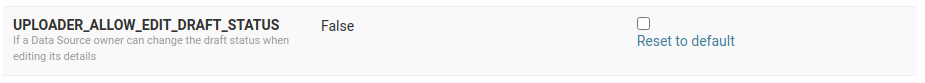
\includegraphics{images/customizations/constance-draft.png}

Them an additional draft field will be available on the edit data source form.

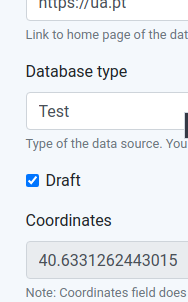
\includegraphics{images/customizations/draft.png}

\hypertarget{development-instructions}{%
\chapter{Development Instructions}\label{development-instructions}}

\hypertarget{repository-structure-description}{%
\subsection*{Repository Structure Description}\label{repository-structure-description}}
\addcontentsline{toc}{subsection}{Repository Structure Description}

\begin{itemize}
\item
  \textbf{backups}: Scripts and configuration files to perform backups of all the data involved in the Network Dashboards applications (Dashboard viewer + Superset)
\item
  \textbf{dashboard\_viewer}: The Dashboard Viewer Django application to manage and upload catalogue results data. More detail can be found in the \href{code-documentation.html}{Code Documentation} chapter.
\item
  \textbf{demo}: Files that can be used to test some processes of the platform (Upload catalogue results data and import a simple dashboard)
\item
  \textbf{docker}: Docker-compose stack-related directories.

  \begin{itemize}
  \tightlist
  \item
    Environment file
  \item
    Configuration directories (Nginx and Postgres)
  \item
    Custom Superest Dockerfile
  \end{itemize}

  For more information about docker deployment consult the \href{installation.html}{Installation} chapter.
\item
  \textbf{docs}: Where the files of this gitbook are hosted. Other output formats can also be obtained here. Consult the \href{development-instructions.html\#documentation}{Documentation} section of this chapter for more details.
\item
  \textbf{superset}: contains a submodule to the latest supported version of Superset's repository and our custom chart plugins
\item
  \textbf{tests}: contains files to launch a docker-compose stack specific to run tests.
\item
  \textbf{requirements-dev}: python requirements files to the several tools to either perform code style checks or to run Django tests
\item
  \textbf{.pre-commit-config.yaml}: configuration for the \href{https://pre-commit.com/}{pre-commit} tool. This is not mandatory to use but is a good tool to automatically fix problems related to code style on staged files
\item
  \textbf{setup.cfg}: configurations for the several code style tools
\item
  \textbf{tox.ini}: configuration for the \href{https://tox.readthedocs.io/}{tox} tool. It helps automate the process to check if the code style is correct and if the Django tests are passing

  It's extremely useful in this context since different code style check tools that we use have some conflicts with python dependencies. It creates a virtual environment for each tox environment, in our case, for each code style check tool plus Django tests
\end{itemize}

\hypertarget{superset}{%
\subsection*{Superset}\label{superset}}
\addcontentsline{toc}{subsection}{Superset}

Currently, we have made some modifications to the box plot visualization on our superset installation which doesn't allow us to use superset's pre-built images available on their docker hub, since we have to call npm's build procedures on the front-end code.
To build our custom docker image we used superset's \href{https://github.com/apache/superset/blob/1.5.0/Dockerfile}{Dockerfile} as a base, where we removed the Dev section and added some code to install our chart plugins before building the front-end code.

The changes made to the Dockerfile to install the chart plugins are in \href{https://github.com/EHDEN/NetworkDashboards/blob/master/docker/superset/Dockerfile\#L47-L49}{this} area:

\begin{enumerate}
\def\labelenumi{\arabic{enumi}.}
\tightlist
\item
  L46: Repalce some boxplot fiels with ours;
\item
  L47: Superset's original version of the controlPanel.ts file is a \texttt{.ts} versions however ours is a \texttt{.tsx}. For that, we have to remove the \texttt{.ts} version to properly override this file.
\end{enumerate}

\hypertarget{update-superset}{%
\subsubsection*{Update Superset}\label{update-superset}}
\addcontentsline{toc}{subsubsection}{Update Superset}

\begin{enumerate}
\def\labelenumi{\arabic{enumi}.}
\item
  \texttt{cd} into superset's submodule directory.
\item
  Get the latest tags: \texttt{git\ fetch\ -t}.
\item
  Checkout to the new desired release tag.
\item
  Check if there are any changes made to superset's Dockerfile (on the root of the repository for the current latest release), adapt them, and insert them on our custom Dockerfile under the \texttt{docker/superset} directory.
\item
  If the version of the plugin package \texttt{plugin-chart-echarts} changed, it's necessary to update our box plot plugin. If it is greater than 0.18.25, go to the history (\texttt{https://github.com/apache/superset/commits/{[}RELEASE-TAG{]}/superset-frontend/plugins/plugin-chart-echarts}) of commits done to the plugin-chart-echarts plugin update to the most recent commit, applying their changes to the files in the \texttt{superset/box-plot-overrides} directory. A fast way check the changes done between two commits: \texttt{git\ diff\ {[}old\_commit\_hash{]}\ {[}recent\_commit\_hash{]}\ -\/-\ superset-frontend/plugins/plugin-chart-echarts}
\end{enumerate}

\hypertarget{chart-plugin-development}{%
\subsubsection*{Chart Plugin Development}\label{chart-plugin-development}}
\addcontentsline{toc}{subsubsection}{Chart Plugin Development}

\begin{enumerate}
\def\labelenumi{\arabic{enumi}.}
\item
  Follow the instructions of \href{https://superset.apache.org/docs/contributing/creating-viz-plugins}{this tutorial} to create the necessary base files of your plugin.
\item
  To deploy you can either use the \texttt{DYNAMIC\_PLUGINS} feature flag or you can add and build your plugins in \texttt{superset/Dockerfile}.
\end{enumerate}

\hypertarget{important-features}{%
\subsubsection*{Important features}\label{important-features}}
\addcontentsline{toc}{subsubsection}{Important features}

\begin{enumerate}
\def\labelenumi{\arabic{enumi}.}
\item
  Standalone Mode: by appending \texttt{?standalone=true} to the URL of a dashboard superset's menu bar won't show.
  New versions support \texttt{?standalone=1} or \texttt{?standalone=2} where the first does the same as \texttt{?standalone=true} and the second also hides the bar containing the name of the dashboard, leaving just the charts.
\item
  Filters:
\end{enumerate}

\begin{itemize}
\tightlist
\item
  check \href{https://superset.apache.org/docs/frequently-asked-questions\#how-to-add-dynamic-filters-to-a-dashboard}{this} faq entry
\item
  Append \texttt{?preselect\_filters=\{"chartId":\{"columnToFilterBy":{[}"value1",\ "value2"{]}\}\}} to the dashboard URL to apply a filter once the dashboard is loaded. E.g. \texttt{?preselect\_filters=\{"13":\{"name":{[}"Demo\ University\ of\ Aveiro"{]}\}\}}
\end{itemize}

\begin{enumerate}
\def\labelenumi{\arabic{enumi}.}
\setcounter{enumi}{2}
\tightlist
\item
  Custom label colors: check \href{https://superset.apache.org/docs/frequently-asked-questions\#is-there-a-way-to-force-the-use-specific-colors}{this} faq entry
\end{enumerate}

\hypertarget{github-actions}{%
\subsection*{Github Actions}\label{github-actions}}
\addcontentsline{toc}{subsection}{Github Actions}

Github has a feature that allows performing automatic actions after a certain event happens on the repository.
We use this feature to execute to check if everything is alright with new PR before merging them to dev.

Github calls a job a set of steps that are executed after a certain event.
Then several jobs can be groups in workflows.
Events are defined at the workflow level, so all the jobs in a workflow will execute at the same time.

We have two workflows:

\begin{enumerate}
\def\labelenumi{\arabic{enumi}.}
\tightlist
\item
  Code analysis checks
\item
  Django tests
\end{enumerate}

The first has three jobs

\begin{enumerate}
\def\labelenumi{\arabic{enumi}.}
\tightlist
\item
  \href{https://github.com/psf/black}{black}: ensures that python's code format is consistent throughout the project
\item
  \href{https://github.com/PyCQA/isort}{isort}: sorts and organizes import statements
\item
  \href{https://github.com/PyCQA/prospector}{prospector}: executes a set of tools that perform some code analysis
\end{enumerate}

The second has just one job that executes the Django tests.

Both workflows execute on commits of pull requests that will be merged into the dev branch.

Regarding the code analysis workflow, the three tools used have requirements that conflict with each other, for that there is a requirements file for each tool on the \texttt{requirement-dev} directory of the repository.
To avoid having three different virtual environments for each tool, you can use the \href{https://tox.readthedocs.io/}{tox}.
You just need to install the development requirements (\texttt{pip\ install\ -r\ requirements-dev/requirements-dev.txt}) and then just run \texttt{tox}.
It will manage the necessary virtual environments and install the requirements for each tool.
If you, however, want to run a specific tool manually you can check the tox configuration file (\href{https://github.com/EHDEN/NetworkDashboards/blob/master/tox.ini}{tox.ini}).
For example for the prospector tool the tox configuration is the following:

\begin{verbatim}
[testenv:prospector]
basepython = python3.8
deps =
    -r{toxinidir}/requirements-dev/requirements-prospector.txt
    -r{toxinidir}/dashboard_viewer/requirements.txt
commands =
    prospector dashboard_viewer
    prospector docker/superset
\end{verbatim}

we can see that it installs the requirement for the prospector tool and also the requirements of the Dashboard Viewer Django app and then runs two commands.

For both black and isort tools, when you run tox, it will show the necessary changes that are required to make the code good.
You can apply the changes automatically by executing the tools manually without the \texttt{-\/-check} and \texttt{-\/-check-only} options respectively.

Sometimes prospector can be a pain in the boot, complaining about too much stuff.
You can make prospector ignore some bad stuff by adding the comment, \texttt{\#\ noqa}, to the end of the specific line where it is complaining.

\hypertarget{tests}{%
\subsection*{Tests}\label{tests}}
\addcontentsline{toc}{subsection}{Tests}

Our tests use Django's building testing features, which uses unittest under the hood.
Not all featured have tests associated, however, there are already \href{https://github.com/EHDEN/NetworkDashboards/issues?q=is\%3Aissue+is\%3Aopen+label\%3A\%22Test+Use+Case\%22}{some tests scenarios} in mind written as issues on the repository, which have the tag \textbf{Test Use Case}.

To run the tests we set up a docker-compose stack, under the \href{https://github.com/EHDEN/NetworkDashboards/tree/master/tests}{test} directory which has just the necessary data containers (Redis and Postgres) to avoid having to make changes on the development/production docker-compose stack.
Once the stack is up it only necessary to run \texttt{SECRET\_KEY=secret\ python\ manage.py\ test} to execute the tests.
If you are developing any tests that involve \href{https://github.com/celery/celery}{celery}, there is no need to have a celery process running, since on Django's settings.py we \href{https://github.com/EHDEN/NetworkDashboards/blob/master/dashboard_viewer/dashboard_viewer/settings.py\#L316}{set the test runner} to the celery one.
This way the \texttt{python\ manage.py\ test} is enough to test the whole application.

\hypertarget{python-requirements}{%
\subsection*{Python Requirements}\label{python-requirements}}
\addcontentsline{toc}{subsection}{Python Requirements}

The python requirements for the Dashboard Viewer Django app are present on the \texttt{requirements.txt} file of the \texttt{dashboard\_viewer} directory.
The file is divided into two sections.
First are the direct dependencies.
Dependencies that are directly used or imported by the Dashboard Viewer Django app.
For better maintainability, every direct dependency has a small description in front of it, so any developer knows why it is being mentioned in the requirements file.
The second part of the file contains the indirect dependencies.
Basically dependencies of our direct dependencies.

After any update is made to the direct dependencies the following procedure should be followed:

\begin{enumerate}
\def\labelenumi{\arabic{enumi}.}
\tightlist
\item
  Create a new virtual environment just for the dependencies of this file
\item
  Delete the indirect dependencies section of the file
\item
  Install all the direct dependencies \texttt{pip\ install\ -r\ requirements.txt}
\item
  Append the result of pip's freeze to the requirements file \texttt{pip\ freeze\ \textgreater{}\textgreater{}\ requirements.txt}
\item
  Remove from the second section of the file, duplicated entries of the first section of the file, in other words, remove from the indirect dependencies section the direct dependencies.
\end{enumerate}

With \href{https://github.com/EHDEN/NetworkDashboards/pull/185}{\#185} we intend to start using the \href{https://github.com/jazzband/pip-tools}{pip-compile} tool.
With it, we can have a file with the direct dependencies (requirements.in), and then pip-compile reads that file and automatically creates a requirements.txt file with all the dependencies and which package requires that specific dependency.
The update process of dependencies will then just be

\begin{enumerate}
\def\labelenumi{\arabic{enumi}.}
\tightlist
\item
  Install the pip-compile tool \texttt{pip\ install\ pip-tools}
\item
  Make the change to the direct dependencies on the requirements.in file (No need for a virtual environment)
\item
  Call the pip-compile tool on the requirement.in file \texttt{pip-compile\ requirements.in}
\end{enumerate}

\hypertarget{documentation}{%
\subsection*{Documentation}\label{documentation}}
\addcontentsline{toc}{subsection}{Documentation}

The plan is to have all the documentation on this git book and any other places that might require some description/information should point to this GitBook so we maintain a commonplace for all the documentation.
This way we can make sure that the code and the documentation are in the same place since on a pull request for a specific feature or a bug fix, associated documentation should also be changed with it.

The manual was written in \href{https://rmarkdown.rstudio.com}{RMarkdown} using the \href{https://bookdown.org}{bookdown} package.
All the code is stored in the \texttt{docs/src} directory as well as the script to build all the documentation.
\textbf{Do not change} the files in the root of the \texttt{docs} directory, because those files will be removed during the build processed and replaced by the new ones.
Therefore, to update this documentation, apply the changes to the files in the directory \texttt{docs/src}.
To build the documentation, you need to have \href{https://www.r-project.org/}{R} installed, and if you are using UNIX-based systems, you only need to run \texttt{sh\ \_build.sh} in the \texttt{docs/src} directory.

In this documentation, we also describe all the settings around the dashboards that are used on the EHDEN project.
To avoid an extensive table of contents and also to avoid having a big chapter page for dashboards, we \href{https://github.com/EHDEN/NetworkDashboards/blob/master/docs/src/_output.yml\#L9}{configured} this GitBook to split different sections into different pages.
A section on the GitBook is mapped to markdown headings elements of level 2 (H2 or \#\#).
This is, however, inconvenient for small chapters like the preface (index.Rmd).
To make it render all the sections on the same page, instead of using headings of level 2 (\#\#) you should use level 3 (\#\#\#).
Although this will make the section numeration start at 0, e.g 1.0.1, 1.0.2, \ldots{}
To avoid this we appended \texttt{\{-\}} to the sections titles so that the numeration does not show.

If a new file is created with more documentation, its name should be placed, including extension, in the desired location in \href{https://github.com/EHDEN/NetworkDashboards/blob/master/docs/src/_bookdown.yml\#L26-L45}{this list} of the \texttt{docks/src/\_bookdown.yml} file.

\hypertarget{code-documentation}{%
\chapter{Code Documentation}\label{code-documentation}}

\hypertarget{apps}{%
\subsection*{Apps}\label{apps}}
\addcontentsline{toc}{subsection}{Apps}

Materialized Queries Manager

Models

This app has only one model, MaterializedQuery, which maps to a Postgres materialized view.
To avoid having to maintain the consistency between both the records of this Django app and the Postgres materialized views:

\begin{itemize}
\tightlist
\item
  the managed Meta flag was set to \texttt{False} to avoid Django creating migrations to the model
\item
  the db\_table Meta flag was set to the name of the table where Postgres stores the information about the existing materialized views (\texttt{pg\_matviews}).
\item
  the fields of the model, matviewname and definition, use the same name and type as the ones of the \texttt{pg\_matviews} Postgres table.
\end{itemize}

Views

This app has no view exposed since all operations to the MaterializedQuery models are expected to be performed in the Django admin app.

However, we had to change Django's default behaviors for the create, update and delete operations of the model.
For the delete operation, we overrode the delete method of the MaterializedQuery Django model to just execute a \texttt{DROP\ MATERIALIZED\ VIEW} SQL statement.
Related to creation and update we had to change some internal methods of Django's admin app ModelAdmin base class.

\begin{enumerate}
\def\labelenumi{\arabic{enumi}.}
\tightlist
\item
  \href{https://github.com/django/django/blob/3.2.5/django/contrib/admin/options.py\#L1542}{\_changeform\_view}: where Model records were being created.
  Instead, \texttt{CREATE\ MATERIALIZED\ VIEW} and \texttt{ALTER\ MATERIALIZED\ VIEW} SQL statements are executed.
  However, since some materialized views might take some time to build, create a record like this could lead to a browser timeout.
  We then decided to execute these statements in a celery background task.
  The main changes were made \href{https://github.com/EHDEN/NetworkDashboards/blob/master/dashboard_viewer/materialized_queries_manager/admin.py\#L87-L92}{here} where we launch the background task.
\item
  \href{https://github.com/django/django/blob/3.2.5/django/contrib/admin/options.py\#L1176}{response\_add}: Since the materialized view might not be created the right way, saying ``A record was created successfully'' is not adequate.
  We then \href{https://github.com/EHDEN/NetworkDashboards/blob/master/dashboard_viewer/materialized_queries_manager/admin.py\#L177-L183}{changed the message} that is presented after the creation to tell in the id of the background task that is creating the materialized query.
  The result of the query can then be consulted on the associated Task Results record on the Celery Results section app of the Django admin console.
\item
  \href{https://github.com/django/django/blob/3.2.5/django/contrib/admin/options.py\#L1253}{response\_change}: changes \href{https://github.com/EHDEN/NetworkDashboards/blob/master/dashboard_viewer/materialized_queries_manager/admin.py\#L213-L219}{here} with the same ideas behind as response\_add.
\end{enumerate}

If any catalogue results files are being uploaded to the platform, any worker attempting to create or change a materialized view will block until such data is uploaded.
Also if any worker is creating materialized views, no other worker can upload catalogue results data.

Through the admin console, there is also the possibility to refresh a specific MaterializedQuery.
To do so, on the list view, select the MaterializedQueries to refresh, then on the actions dropdown select ``Refresh selected materialized queries''.
Once again to avoid timeouts, such operations are executed on a background task.

Tabs Manager

Currently, this app is not being used and the URL mapping was delete.
To use it again uncomment the tabsManager \href{https://github.com/EHDEN/NetworkDashboards/blob/master/dashboard_viewer/dashboard_viewer/urls.py\#L29}{line} on the dashboard\_viewer/dashboard\_viewer/urls.py file.
Then you can access the tabs page through the \texttt{{[}BASE\_URL{]}/tabs/} URL.

Views

On this app, there is only one view.
It is a simple page with just a sidebar to choose which dashboard to displays on an iframe.
Besides the simplicity, all the animations around the sidebar buttons are handled by CSS with some JS that adds and removes classes to HTML elements, as events (hover and click) happen.
To facilitate the development process of CSS, \href{https://sass-lang.com/}{SCSS} was used to build styling of the view.
It prevents duplication with the addition of variables and adds the possibility to express parent classes by nesting their declaration.

In cases where there are a lot of buttons on the sidebar, some buttons might get impossible to reach since they are out of the field of view.
To avoid this we make use of \href{https://github.com/Grsmto/simplebar}{SimpleBar}, which makes the sidebar scrollable, displaying a scroll bar on the right side of the sidebar whenever there are elements outside of the field of view.

API

There is one endpoint, \texttt{{[}BASE\_URL{]}/api/}, where a JSON object of tabs and groups of tabs and their sub-tabs are returned.

Models

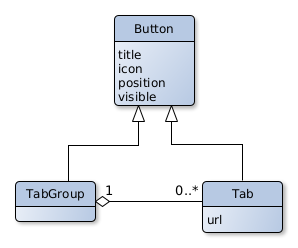
\includegraphics{images/code-documentation/tabs-models.png}

Uploader

Views

This app exposes three views:
1. Creation of a data source
2. Edition of a data source
3. To Upload or consult the history of uploads of catalogue results files.

The first one can be accessed through the \texttt{{[}BASE\_URL{]}/uploader/{[}DATA\_SOURCE\_HASH{]}/} URL.

\begin{itemize}
\tightlist
\item
  If no hash is provided on the URL then on the creation of the data source a random one will be assigned.
\item
  If there is already a data source with the provided hash then the user is redirected to the upload page of that data source.
\end{itemize}

This view also allows creating data sources without displaying the webform, redirecting directly to the uploader page.
This can be achieved by providing the data of several fields of the form as URL arguments.
E.g. \texttt{{[}BASE\_URL{]}/uploader/{[}DATA\_SOURCE\_HASH{]}/?acronym=test...}.
This is implemented in a way so that whenever a GET is performed, it checks the URL arguments and tries to submit the data source form.
If it is valid, all the required fields were provided and are valid, then the user is redirected to the upload page.
Else all the valid values are set in the form, the invalid ones are being discarded, and the data source creation page is presented with no error messages.
The country field should contain a value from the ones available on the dropdown presented in the webform and since the coordinates is a two-component value it should be provided as \texttt{coordinates\_0={[}LATITUDE{]}\&coordinates\_1={[}LONGITUDE{]}}.
It is important to note that this view does not require a CSRF token, so a normal POST form submission can be performed to create a data source.

\begin{center}\rule{0.5\linewidth}{0.5pt}\end{center}

The second one can be accessed through the \texttt{{[}BASE\_URL{]}/uploader/{[}DATA\_SOURCE\_HASH{]}/edit/} URL or by clicking on the Edit button on the data source upload page.

\begin{center}\rule{0.5\linewidth}{0.5pt}\end{center}

Finally, on the upload page, a data owner can consult the history of uploads, their state, and eventually error messages if some went wrong.
Whenever an upload is made its state will be pending.
After the upload, with a 5-second interval, a request is made to the backend to check if the status of the upload changed.
If it fails, an error message will be provided in a tooltip above a button with a message icon.
Else the state will change to Done and the information about the upload retrieved from the uploaded file, present on the check status request, is filled.

Related to file uploading, after the file form is submitted no validation is made and a message is presented to the user telling that the file is being processed in the background, then the fetch status process mentioned before starts.
If validations were performed before returning a message to the user, if the validation took too much time, the browser could timeout.
Also if some unexpected error happened on the insertion process performed in the background, the user would get any feedback.

Related to the background task that validates and uploads the data, the validation can fail if:

\begin{longtable}[]{@{}cc@{}}
\toprule
\begin{minipage}[b]{0.47\columnwidth}\centering
Error\strut
\end{minipage} & \begin{minipage}[b]{0.47\columnwidth}\centering
Message\strut
\end{minipage}\tabularnewline
\midrule
\endhead
\begin{minipage}[t]{0.47\columnwidth}\centering
Invalid Number of Columns\strut
\end{minipage} & \begin{minipage}[t]{0.47\columnwidth}\centering
The provided file has an invalid number of columns\strut
\end{minipage}\tabularnewline
\begin{minipage}[t]{0.47\columnwidth}\centering
Invalid CSV File Format\strut
\end{minipage} & \begin{minipage}[t]{0.47\columnwidth}\centering
The provided file has an invalid CSV format. Make sure is a text file separated by commas and you either have 7 (regular results file) or 13 (results file with dist columns) columns.\strut
\end{minipage}\tabularnewline
\begin{minipage}[t]{0.47\columnwidth}\centering
Missing Required Fields\strut
\end{minipage} & \begin{minipage}[t]{0.47\columnwidth}\centering
Some rows have null values either on the column ``analysis\_id'' or ``count\_value''\strut
\end{minipage}\tabularnewline
\begin{minipage}[t]{0.47\columnwidth}\centering
Invalid Field Types\strut
\end{minipage} & \begin{minipage}[t]{0.47\columnwidth}\centering
The provided file has invalid values on some columns. Remember that only the "stratum\_*" columns accept strings, all the other fields expect numeric types.\strut
\end{minipage}\tabularnewline
\begin{minipage}[t]{0.47\columnwidth}\centering
Duplicated Metadata Rows\strut
\end{minipage} & \begin{minipage}[t]{0.47\columnwidth}\centering
Analysis id{[}output{]} duplicated on multiple rows. Try (re)running the plugin CatalogueExport on your database.\strut
\end{minipage}\tabularnewline
\begin{minipage}[t]{0.47\columnwidth}\centering
Missing Required Metadata Row\strut
\end{minipage} & \begin{minipage}[t]{0.47\columnwidth}\centering
Analysis id 0 is missing. Try (re)running the plugin CatalogueExport on your database.\strut
\end{minipage}\tabularnewline
\bottomrule
\end{longtable}

Any other error is considered an unexpected error and the following message will be presented ``An unexpected error occurred while processing your file. Please contact the system administrator for more details.''.

If the file passes all validations, it goes to the upload data phase.
Here, if workers are creating or refreshing materialized queries then the worker blocks.
If there are other workers inserting data for the same data source it will also block.
However, several workers of different data sources can insert data at the same time.
All the workers, after inserting the data, check if they are the only worker inserting data. If so they refresh the existing materialized queries.
Else the next worker to finish inserting data will do the same check.

Widgets

For the data source form two custom widgets were created for the following fields:

\begin{itemize}
\tightlist
\item
  Database Type: To avoid having duplicate entries with the same meaning (e.g.~Hospital, hospital), the input of this field has a autocomplete list where existing values are suggested to the user.
  Also before saving the field to the database spaces are trimmed and the values are transformed into title case \href{https://github.com/EHDEN/NetworkDashboards/blob/master/dashboard_viewer/uploader/forms.py\#L25}{here}.
\item
  Coordinates: 1. This is a two-component field; 2. Inserting coordinates by hand is tedious. Considering the previous points, we created a widget with a map built with \href{https://leafletjs.com/}{leaflet} where the user just needs to click on the map.
\end{itemize}

API

This app provided two API endpoints

\begin{enumerate}
\def\labelenumi{\arabic{enumi}.}
\item
  Update data source information: a PATCH request with a JSON object on the body of the request with the fields and their new values.
\item
  Pending upload status: a GET request that returns JSON data where there is always a \texttt{status} field that can have three statuses which then can lead to additional data be also present:
\end{enumerate}

\begin{itemize}
\tightlist
\item
  Pending: the upload in question hasn't finished
\item
  Done: the upload finished and there was nothing wrong with the uploaded file.
  Along with the status, there will be a \texttt{data} field with a JSON object with the fields \texttt{r\_package\_version}, \texttt{generation\_date}, \texttt{cdm\_version}, and \texttt{vocabulary\_version} which are data source information that was extracted from the uploaded file.
\item
  Failed: the upload finished but there was something wrong with the uploaded file.
  Along with the status, there will be a \texttt{failure\_msg} field telling the reason for the failure.
\end{itemize}

Models

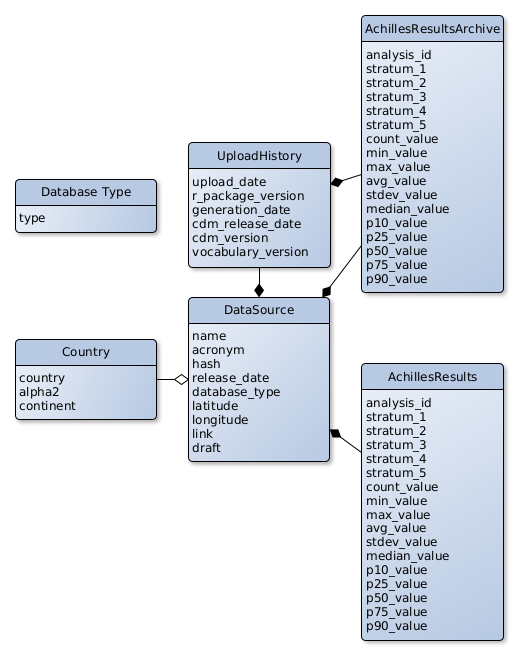
\includegraphics{images/code-documentation/uploader-models.png}

\begin{itemize}
\tightlist
\item
  Country data is loaded in a fresh installation through the \href{https://github.com/EHDEN/NetworkDashboards/blob/master/dashboard_viewer/docker-init.sh}{docker-init.sh} script if no records are present on the Country table.
\item
  The DataSource model doesn't have a foreign key to the DatabaseType model to then facilitate the creation of SQL queries to feet Superset's dashboards.
  The DatabaseType is used anyway to have a faster way to check if a certain database type already exists on the database, avoiding going through every DataSource record.
\item
  The same situation of the DatabaseType model also happens between the UploadHistory and PendingUpload models.
  There is no foreign key between a UploadHistory and a PendingUpload.
  This is because PendingUpload records are deleted once an upload is successful.
  When the upload view requests the status of a certain upload, it uses the id of the pending upload.
  If no pending upload is found, it is assumed that the upload was successful and searches for uploads on the UploadHistory model with the pending\_upload\_id field equal to the certain upload id.
  Related to where the uploaded files are stored, within the media directory there will be a \href{https://github.com/EHDEN/NetworkDashboards/blob/master/dashboard_viewer/dashboard_viewer/settings.py\#L198}{ACHILLES\_RESULTS\_STORAGE\_PATH} directory which will have a directory for each data source.
  Within this last directory, first, files are uploaded to a \texttt{failure} directory.
  If the upload is successful the file is moved to a success directory.
  In both cases, the file name will be the date of when the file is being saved into disk plus its original extensions.
\end{itemize}

\hypertarget{javascript-packages}{%
\subsection*{JavaScript Packages}\label{javascript-packages}}
\addcontentsline{toc}{subsection}{JavaScript Packages}

While developing the templates for Django views, if a certain javascript library is required, like jquery, one option is to insert \texttt{script} tags on the templates and point the src to a CDN.
However, this makes the process of maintaining the libraries tedious since a developer has to search and change all the \texttt{script} tags if for example wants to update the library's version.
To avoid this problem we have a \texttt{package.json} file where we define all the libraries that we use and their version.
Then we \href{https://github.com/EHDEN/NetworkDashboards/blob/master/dashboard_viewer/dashboard_viewer/settings.py\#L182}{add} the \texttt{node\_modules} directory as a static file directory.
With this alternative, updating a library is as simple as changing a number of the \texttt{package.json} file, run \texttt{npm\ install} and collect the static files again.

\hypertarget{dashboards}{%
\chapter{Dashboards}\label{dashboards}}

\hypertarget{PerDatabaseDashboard}{%
\section{Network Dashboard}\label{PerDatabaseDashboard}}

\hypertarget{label-colors}{%
\subsection*{Label Colors}\label{label-colors}}
\addcontentsline{toc}{subsection}{Label Colors}

In order to obtain the colors blue and rose in the chart representing the gender distribution,
add the following JSON entry to the JSON object of the \texttt{JSON\ Metadata} field on the edit dashboard page:

\begin{Shaded}
\begin{Highlighting}[]
\ErrorTok{"label\_colors":} \FunctionTok{\{}
    \DataTypeTok{"Male"}\FunctionTok{:} \StringTok{"\#3366FF"}\FunctionTok{,} 
    \DataTypeTok{"Female"}\FunctionTok{:} \StringTok{"\#FF3399"}
\FunctionTok{\}}
\end{Highlighting}
\end{Shaded}

\hypertarget{css}{%
\subsection*{CSS}\label{css}}
\addcontentsline{toc}{subsection}{CSS}

To hide the dashboard header insert the following css code to the \texttt{CSS} field on the edit page:

\begin{Shaded}
\begin{Highlighting}[]
\FunctionTok{.dashboard} \OperatorTok{\textgreater{}}\NormalTok{ div}\InformationTok{:not(}\FunctionTok{.dashboard{-}content}\InformationTok{)}\NormalTok{ \{  }\CommentTok{/* dashboard header */}
  \KeywordTok{display}\NormalTok{: }\DecValTok{none}\OperatorTok{;}
\NormalTok{\}}
\end{Highlighting}
\end{Shaded}

With this every time you want to edit the dashboard layout you have to either comment the CSS inserted
or remove it so the ``Edit Dashboard'' button can show again.

\hypertarget{filters}{%
\subsection*{Filters}\label{filters}}
\addcontentsline{toc}{subsection}{Filters}

\hypertarget{country-filter}{%
\subsubsection*{Country Filter}\label{country-filter}}
\addcontentsline{toc}{subsubsection}{Country Filter}

Dataset: Materialized View \href{materialized-views-1.html\#meta_data_table}{meta\_data\_table}

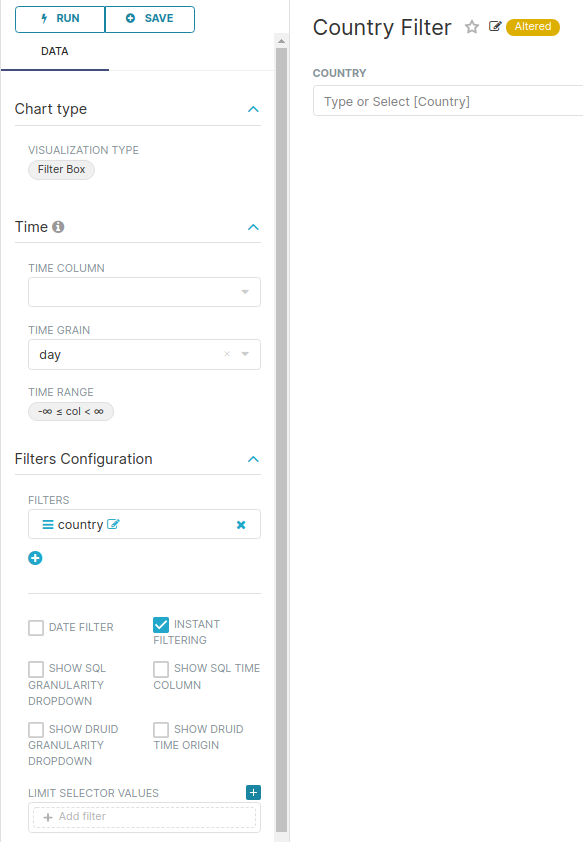
\includegraphics{images/11-network-dashboard/01-filters/01-country.png}

\hypertarget{database-type-filter}{%
\subsubsection*{Database Type Filter}\label{database-type-filter}}
\addcontentsline{toc}{subsubsection}{Database Type Filter}

Dataset: Materialized View \href{materialized-views-1.html\#meta_data_table}{meta\_data\_table}

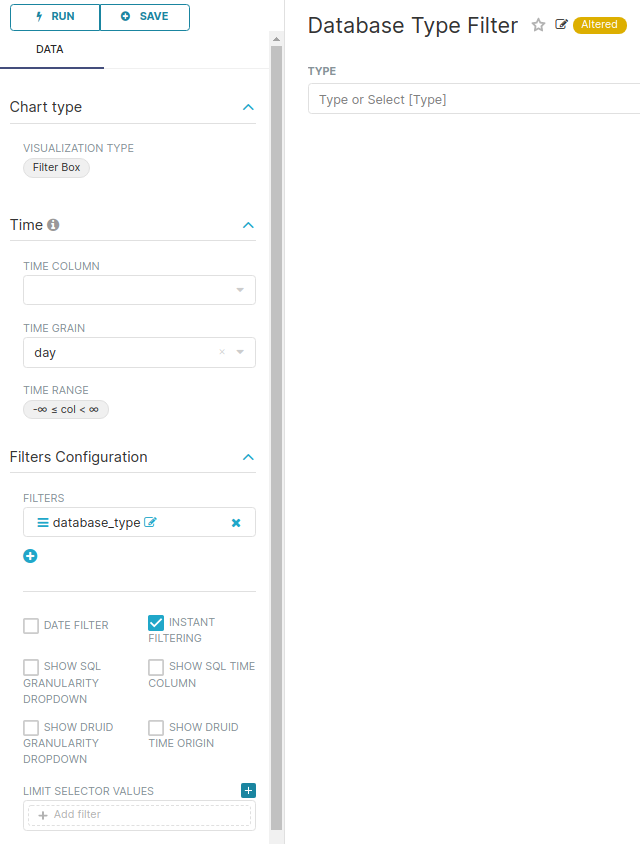
\includegraphics{images/11-network-dashboard/01-filters/02-database-type.png}

\hypertarget{data-source-filter}{%
\subsubsection*{Data Source Filter}\label{data-source-filter}}
\addcontentsline{toc}{subsubsection}{Data Source Filter}

Dataset: Materialized View \href{materialized-views-1.html\#meta_data_table}{meta\_data\_table}

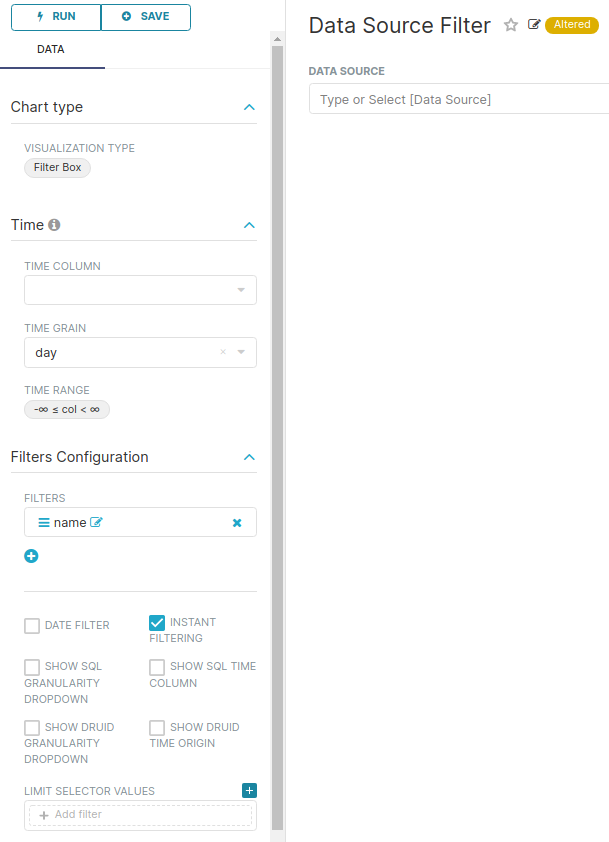
\includegraphics{images/11-network-dashboard/01-filters/03-datasource.png}

\hypertarget{overview-tab}{%
\subsection*{Overview Tab}\label{overview-tab}}
\addcontentsline{toc}{subsection}{Overview Tab}

\hypertarget{countries}{%
\subsubsection*{Countries}\label{countries}}
\addcontentsline{toc}{subsubsection}{Countries}

Dataset: Materialized View \href{materialized-views-1.html\#meta_data_table}{meta\_data\_table}

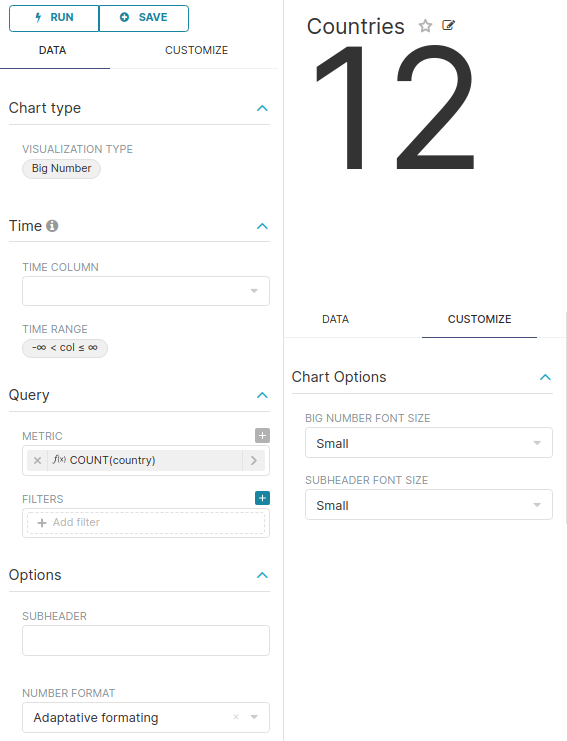
\includegraphics{images/11-network-dashboard/02-overview/01-countries.png}

\hypertarget{data-sources-1}{%
\subsubsection*{Data Sources}\label{data-sources-1}}
\addcontentsline{toc}{subsubsection}{Data Sources}

Dataset: Materialized View \href{materialized-views-1.html\#meta_data_table}{meta\_data\_table}

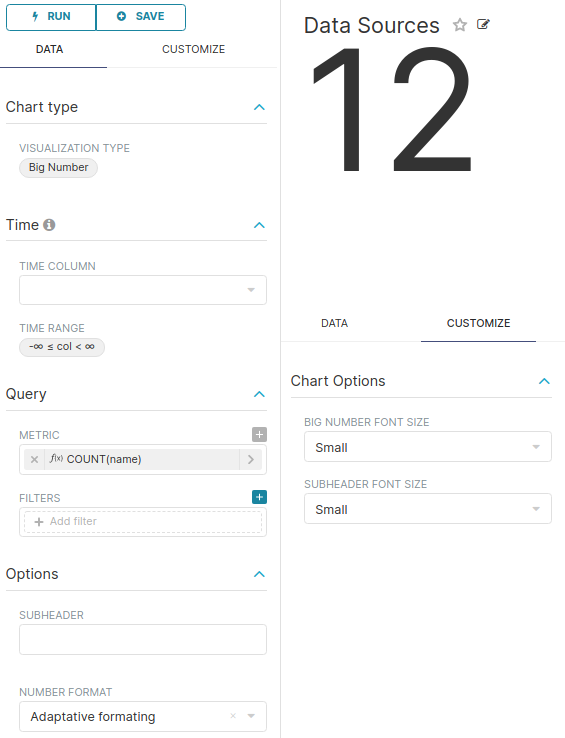
\includegraphics{images/11-network-dashboard/02-overview/02-datasource.png}

\hypertarget{datasource-types}{%
\subsubsection*{Datasource Types}\label{datasource-types}}
\addcontentsline{toc}{subsubsection}{Datasource Types}

Dataset: Materialized View \href{materialized-views-1.html\#meta_data_table}{meta\_data\_table}

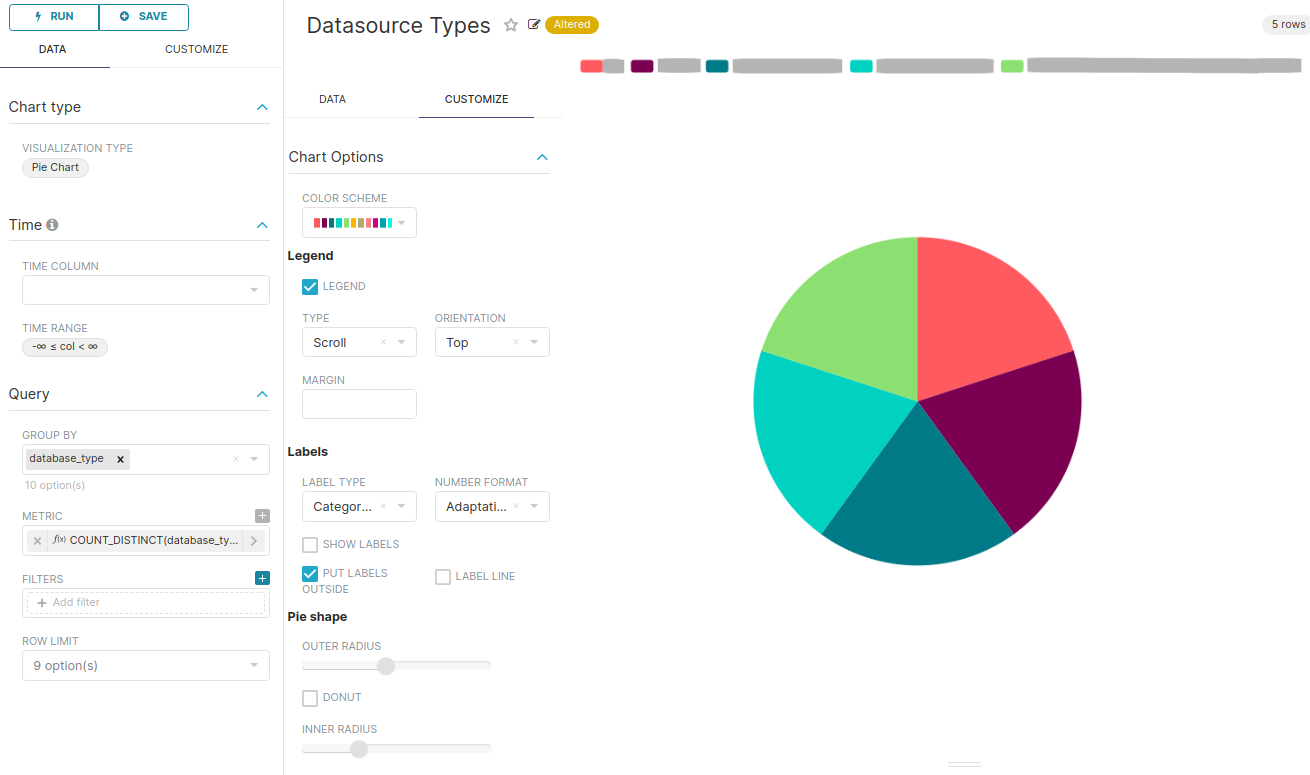
\includegraphics{images/11-network-dashboard/02-overview/03-datasource-type.png}

\hypertarget{patients}{%
\subsubsection*{Patients}\label{patients}}
\addcontentsline{toc}{subsubsection}{Patients}

Dataset: Materialized View \href{materialized-views-1.html\#meta_data_table}{meta\_data\_table}

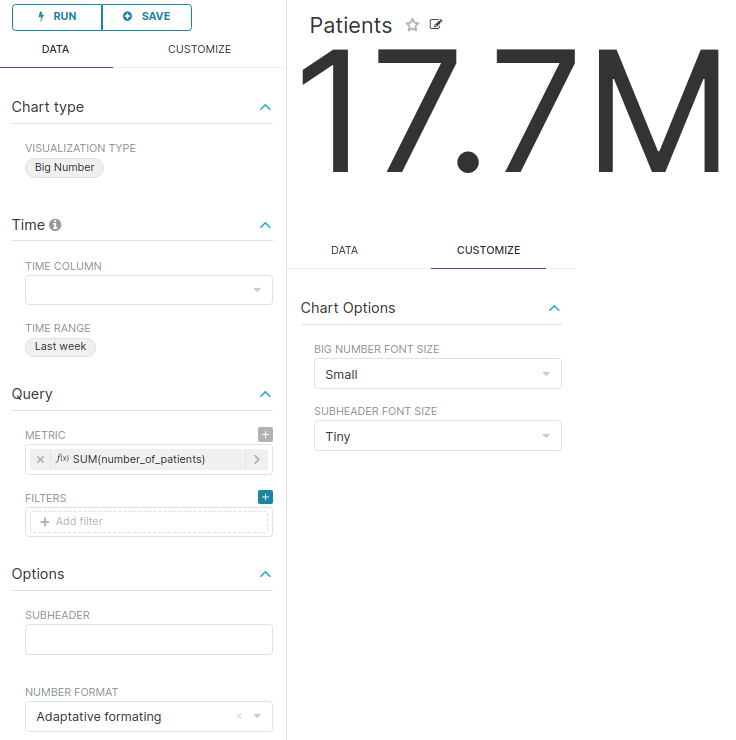
\includegraphics{images/11-network-dashboard/02-overview/04-patients.png}

\hypertarget{patients-1}{%
\subsubsection*{Patients}\label{patients-1}}
\addcontentsline{toc}{subsubsection}{Patients}

Dataset: Materialized View \href{materialized-views-1.html\#meta_data_table}{meta\_data\_table}

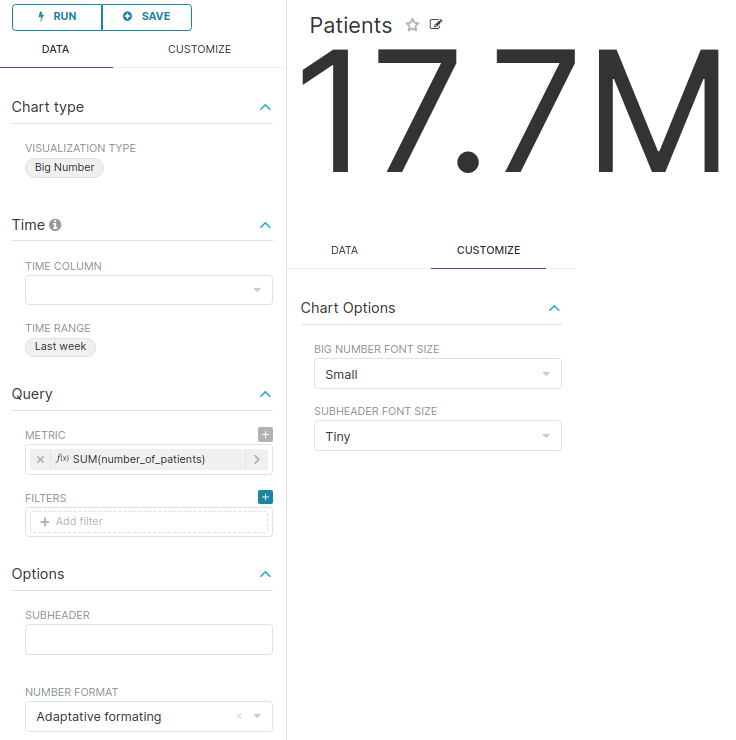
\includegraphics{images/11-network-dashboard/02-overview/04-patients.png}

\hypertarget{patients-by-country}{%
\subsubsection*{Patients by Country}\label{patients-by-country}}
\addcontentsline{toc}{subsubsection}{Patients by Country}

Dataset: Materialized View \href{materialized-views-1.html\#patients_per_country_and_database_type}{meta\_data\_table}

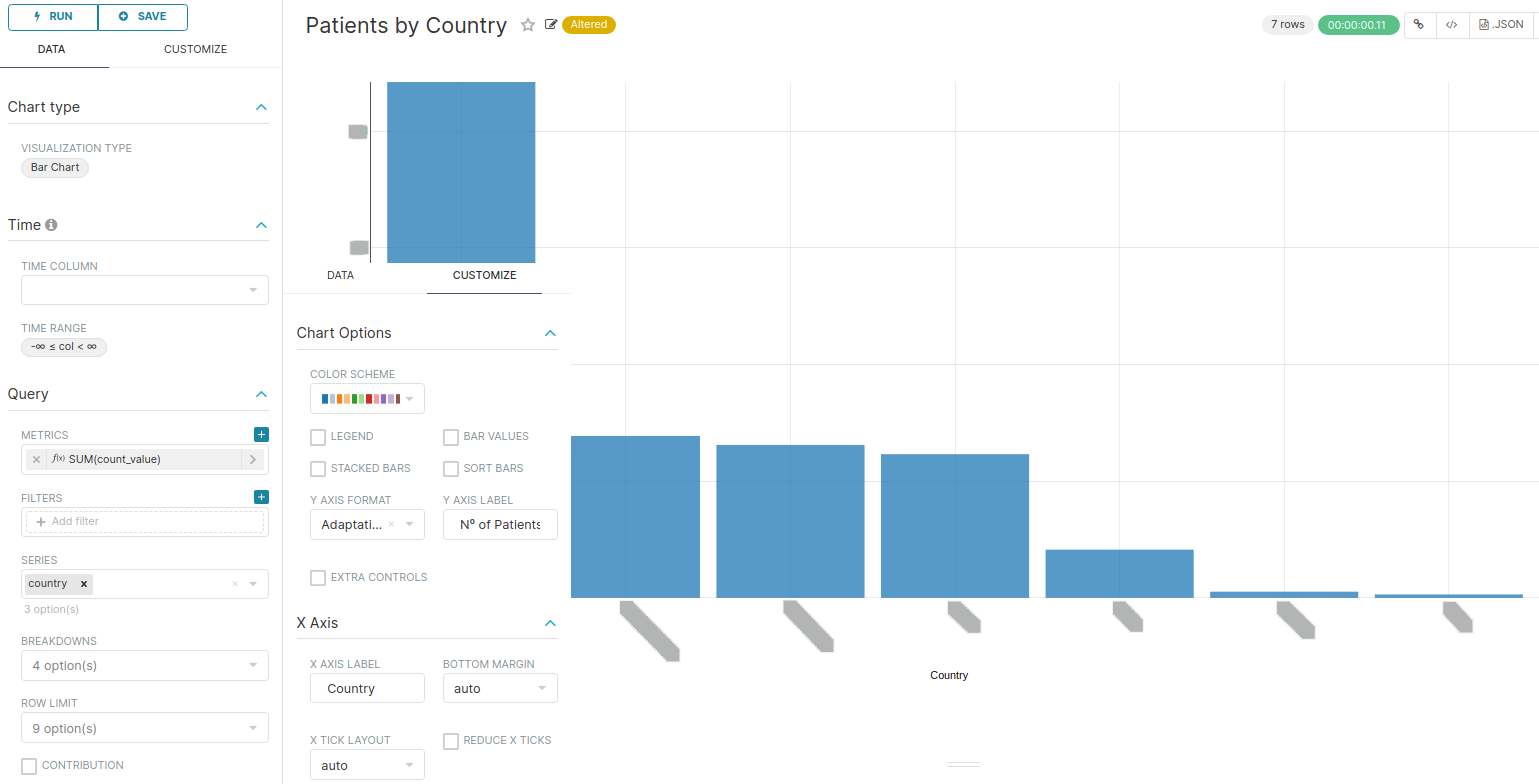
\includegraphics{images/11-network-dashboard/02-overview/05-patients-by-country.png}

\hypertarget{database-types-per-country}{%
\subsubsection*{Database Types per Country}\label{database-types-per-country}}
\addcontentsline{toc}{subsubsection}{Database Types per Country}

Dataset: Materialized View \href{materialized-views-1.html\#patients_per_country_and_database_type}{meta\_data\_table}

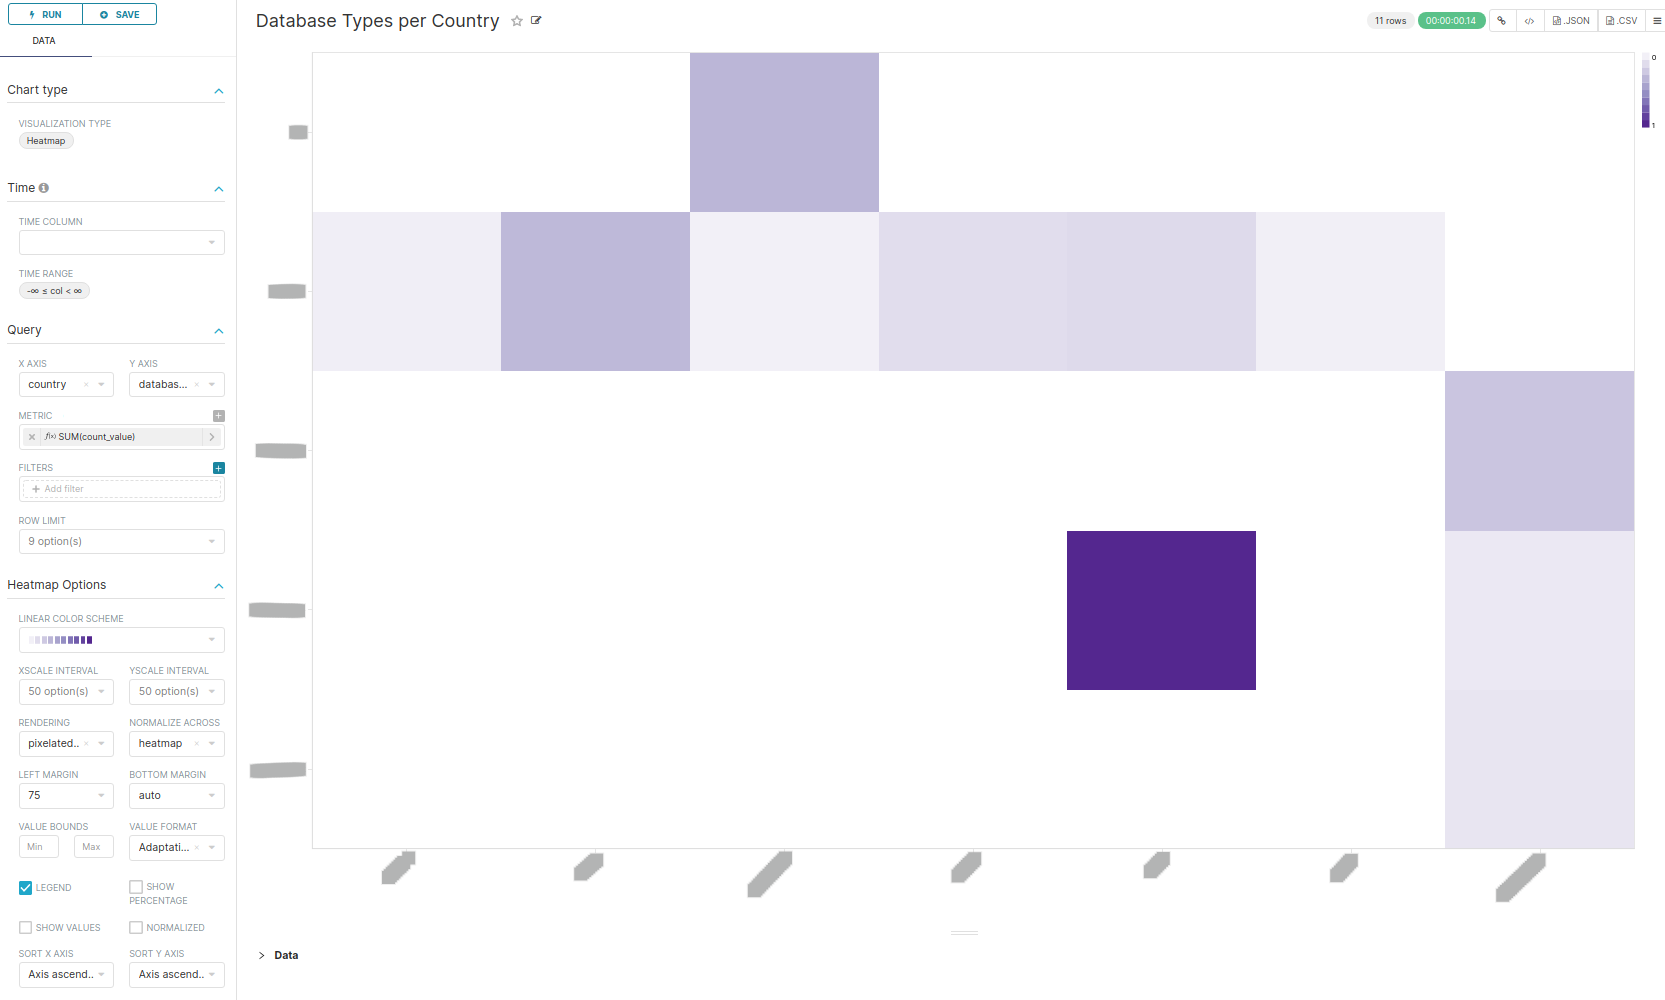
\includegraphics{images/11-network-dashboard/02-overview/06-database-types-by-country.png}

\hypertarget{meta-data}{%
\subsubsection*{Meta Data}\label{meta-data}}
\addcontentsline{toc}{subsubsection}{Meta Data}

Dataset: Materialized View \href{materialized-views-1.html\#meta_data_table}{meta\_data\_table}

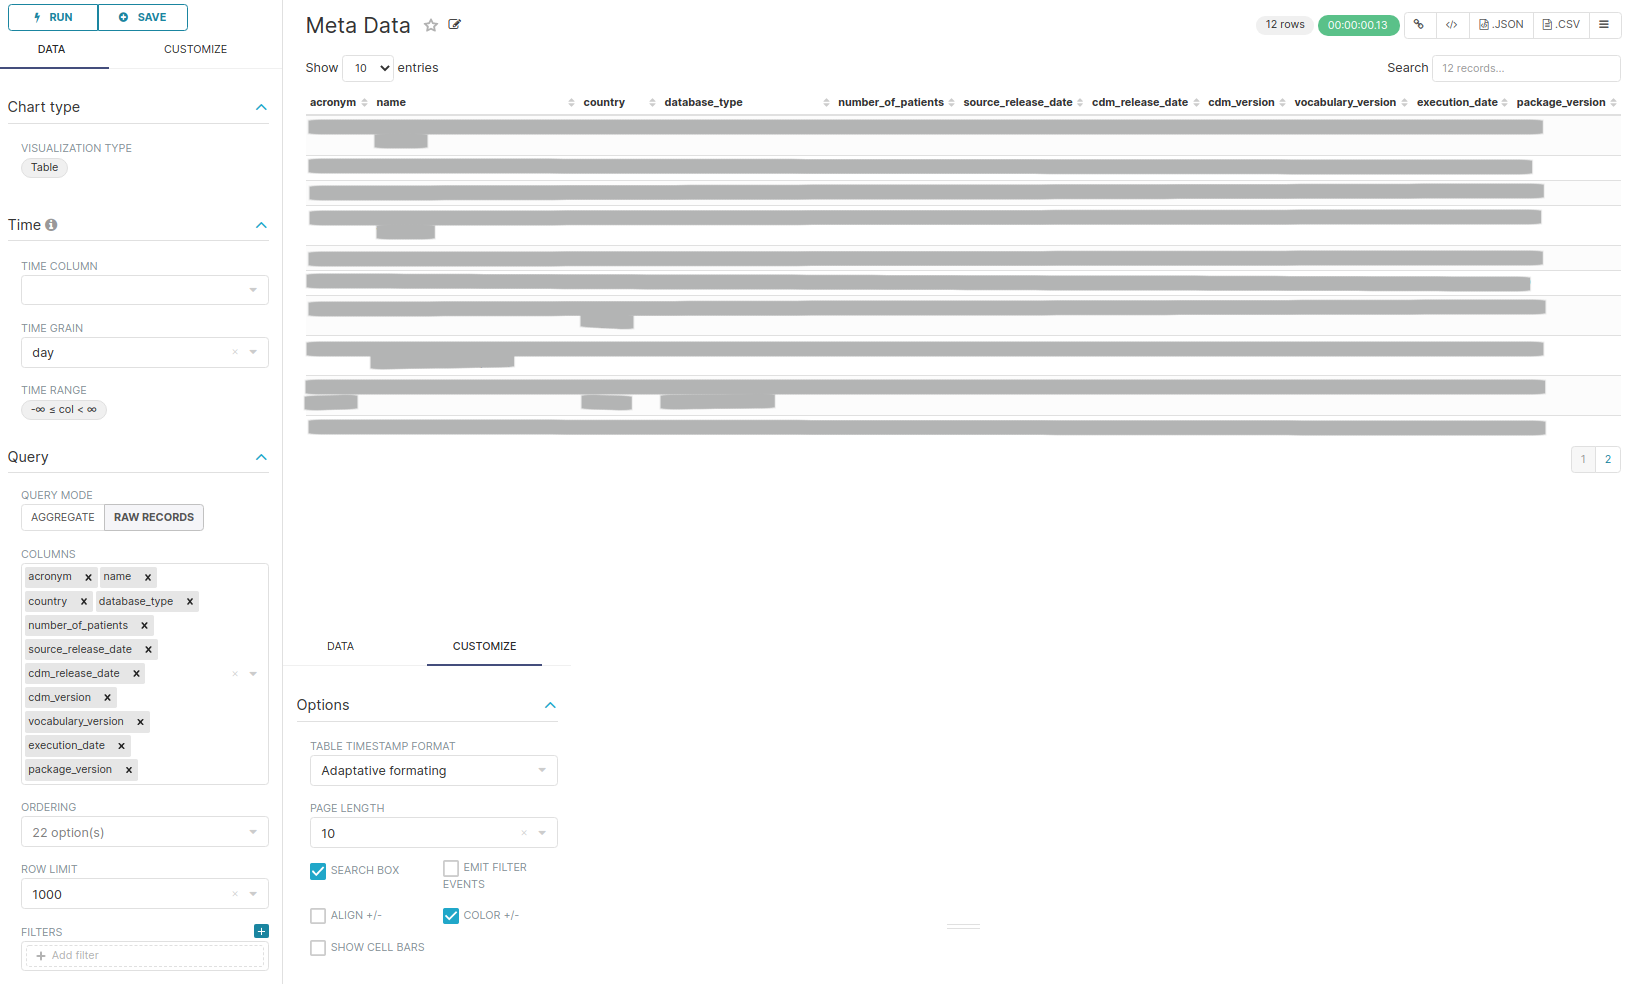
\includegraphics{images/11-network-dashboard/02-overview/07-metadata.png}

\hypertarget{demographics-tab}{%
\subsection*{Demographics Tab}\label{demographics-tab}}
\addcontentsline{toc}{subsection}{Demographics Tab}

\hypertarget{number-of-patients}{%
\subsubsection*{Number of Patients}\label{number-of-patients}}
\addcontentsline{toc}{subsubsection}{Number of Patients}

Dataset: Materialized View \href{materialized-views-1.html\#number_of_patients}{number\_of\_patients}

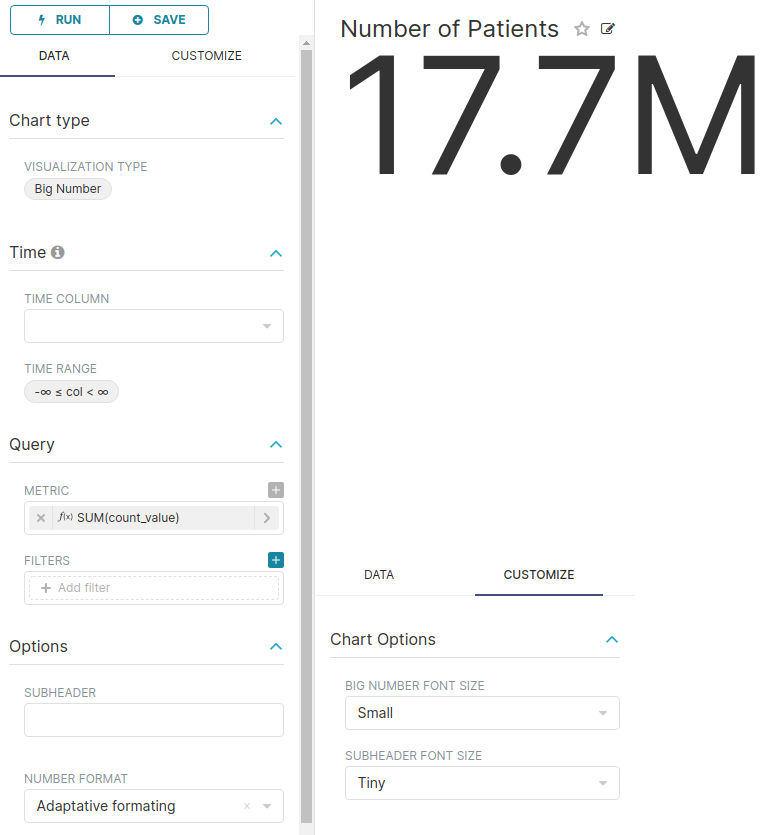
\includegraphics{images/11-network-dashboard/03-demographics/01-number-of-patients.png}

\hypertarget{gender-table}{%
\subsubsection*{Gender Table}\label{gender-table}}
\addcontentsline{toc}{subsubsection}{Gender Table}

Dataset: Materialized View \href{materialized-views-1.html\#gender}{gender}

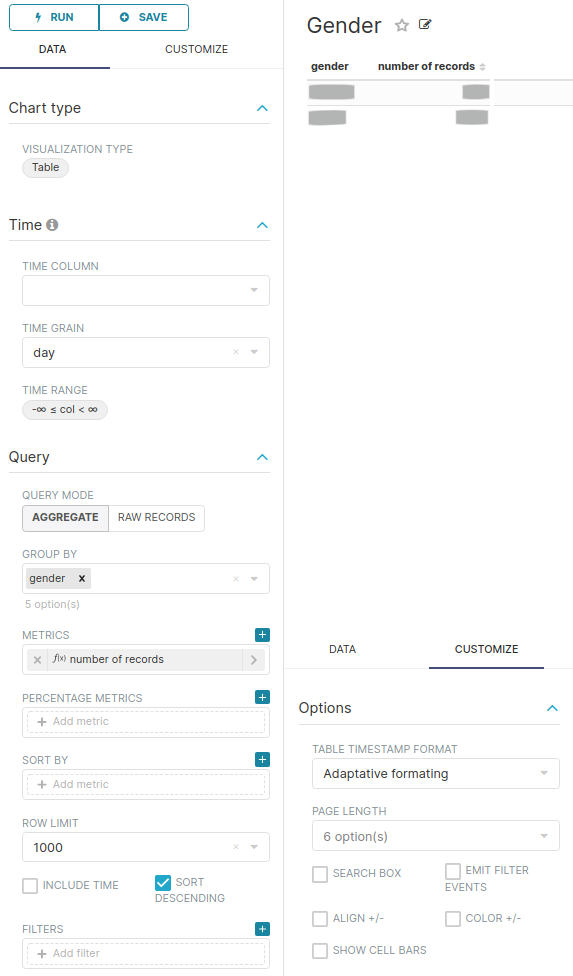
\includegraphics{images/11-network-dashboard/03-demographics/02-gender-table.png}

\hypertarget{gender-pie}{%
\subsubsection*{Gender Pie}\label{gender-pie}}
\addcontentsline{toc}{subsubsection}{Gender Pie}

Dataset: Materialized View \href{materialized-views-1.html\#gender}{gender}

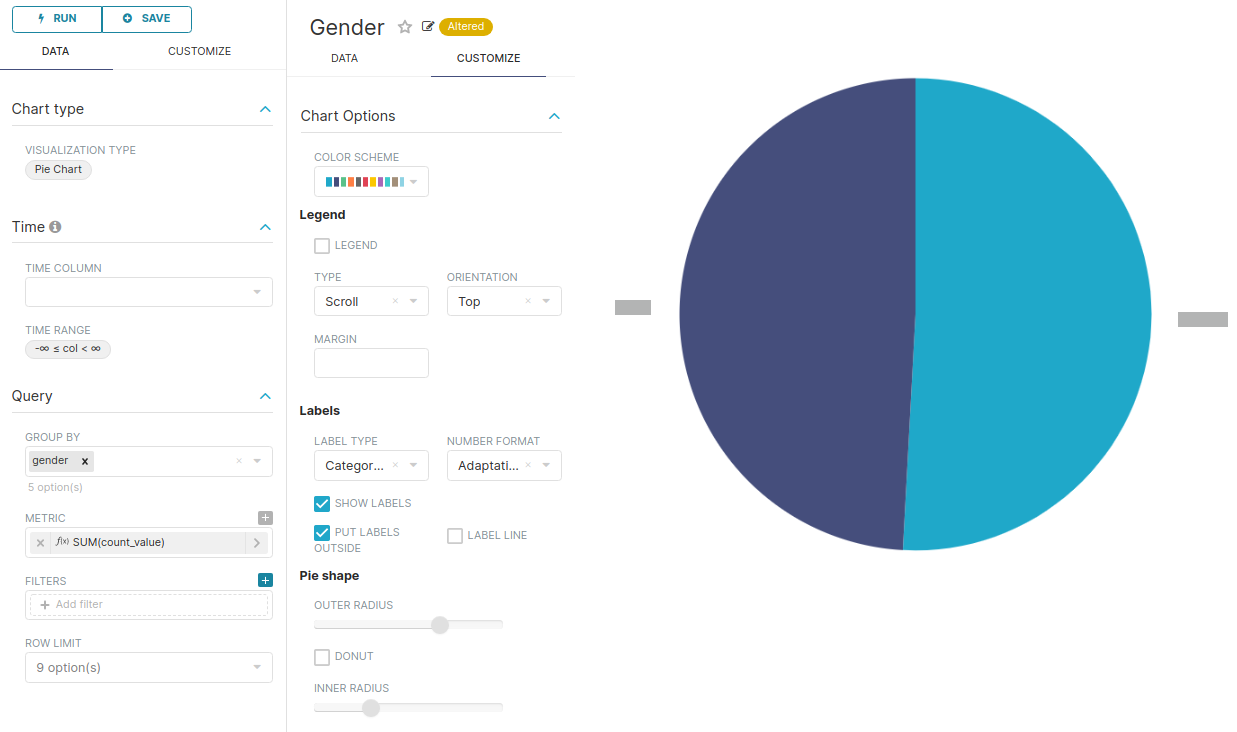
\includegraphics{images/11-network-dashboard/03-demographics/03-gender-pie.png}

\hypertarget{age-at-first-observation-table}{%
\subsubsection*{Age at first observation Table}\label{age-at-first-observation-table}}
\addcontentsline{toc}{subsubsection}{Age at first observation Table}

Dataset: Materialized View \href{materialized-views-1.html\#age1observation_table}{age1observation\_table}

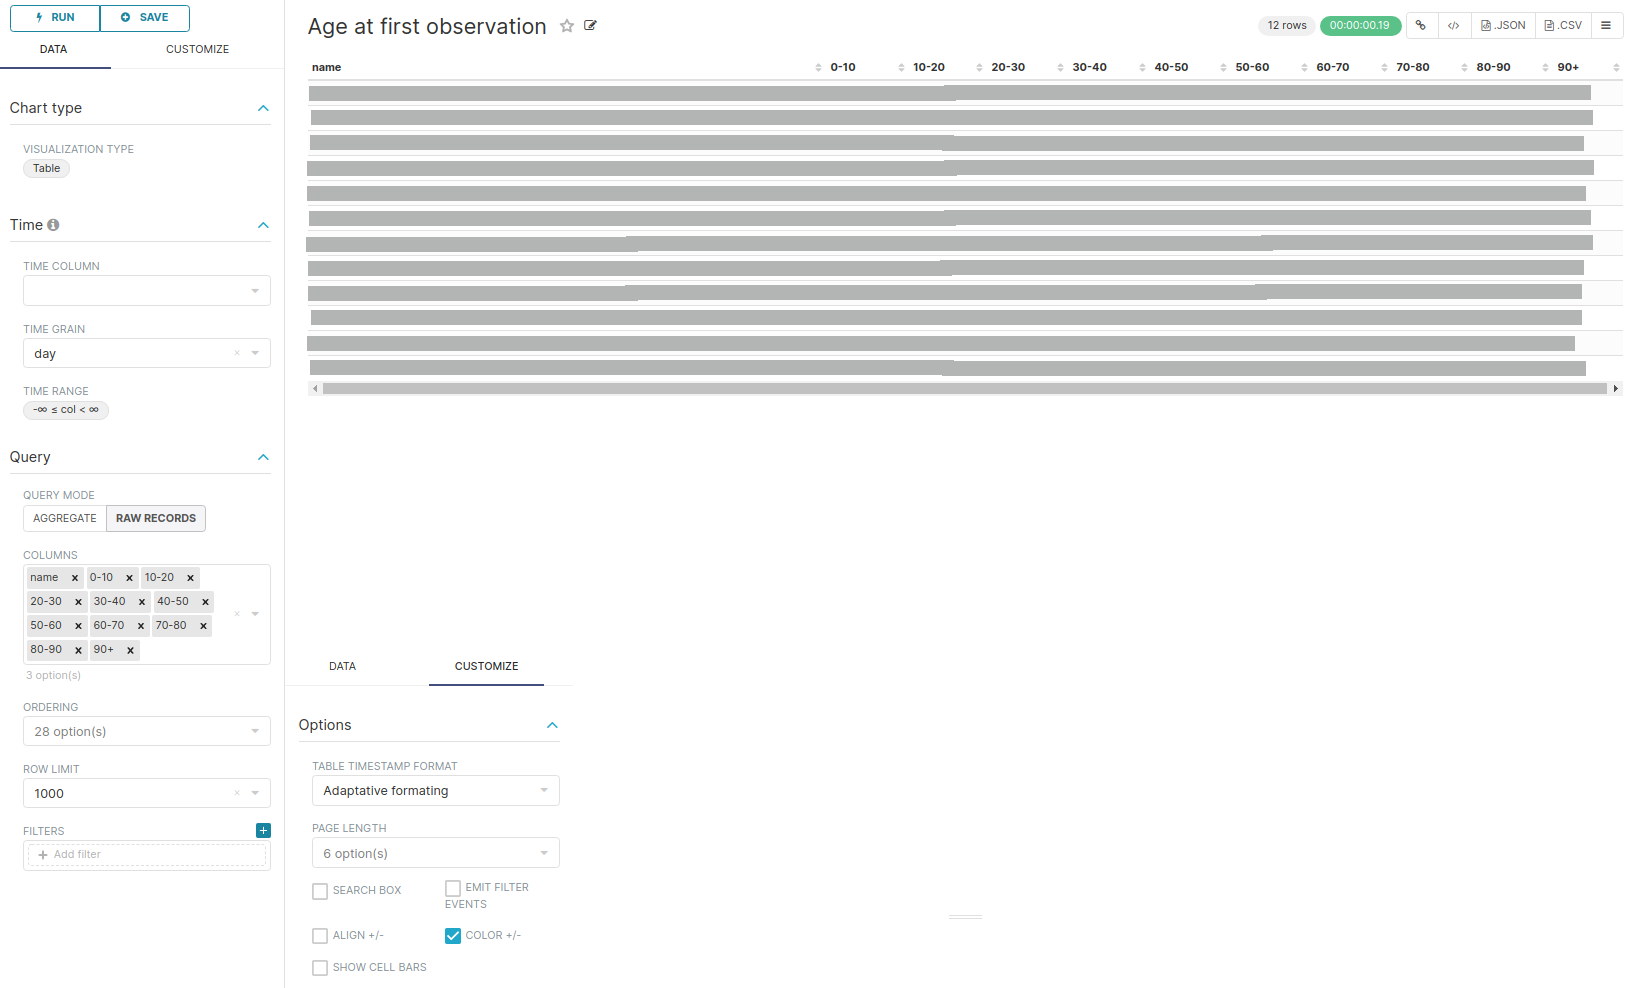
\includegraphics{images/11-network-dashboard/03-demographics/04-age-at-first-observation-table.png}

\hypertarget{age-at-first-observation-bar-chart}{%
\subsubsection*{Age at first observation Bar Chart}\label{age-at-first-observation-bar-chart}}
\addcontentsline{toc}{subsubsection}{Age at first observation Bar Chart}

Dataset: Materialized View \href{materialized-views-1.html\#age1observation_bar_chart}{age1observation\_bar\_chart}

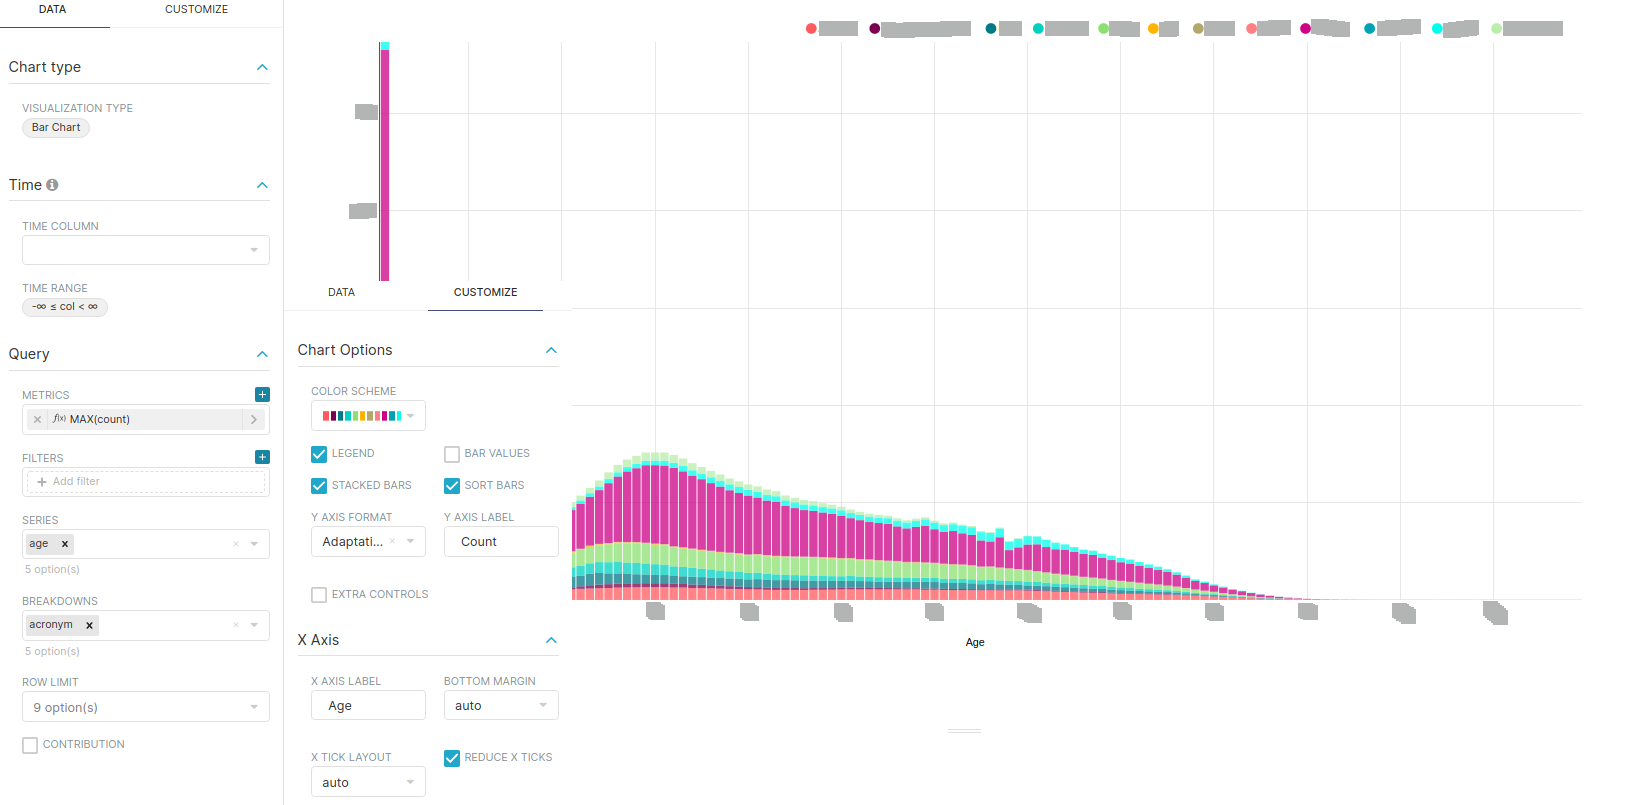
\includegraphics{images/11-network-dashboard/03-demographics/05-age-at-first-observation-bar-chart.png}

\hypertarget{distribution-of-age-at-first-observation-period}{%
\subsubsection*{Distribution of age at first observation period}\label{distribution-of-age-at-first-observation-period}}
\addcontentsline{toc}{subsubsection}{Distribution of age at first observation period}

Dataset: Materialized View \href{materialized-views-1.html\#distribution_of_age_at_first_observation_period}{distribution\_of\_age\_at\_first\_observation\_period}

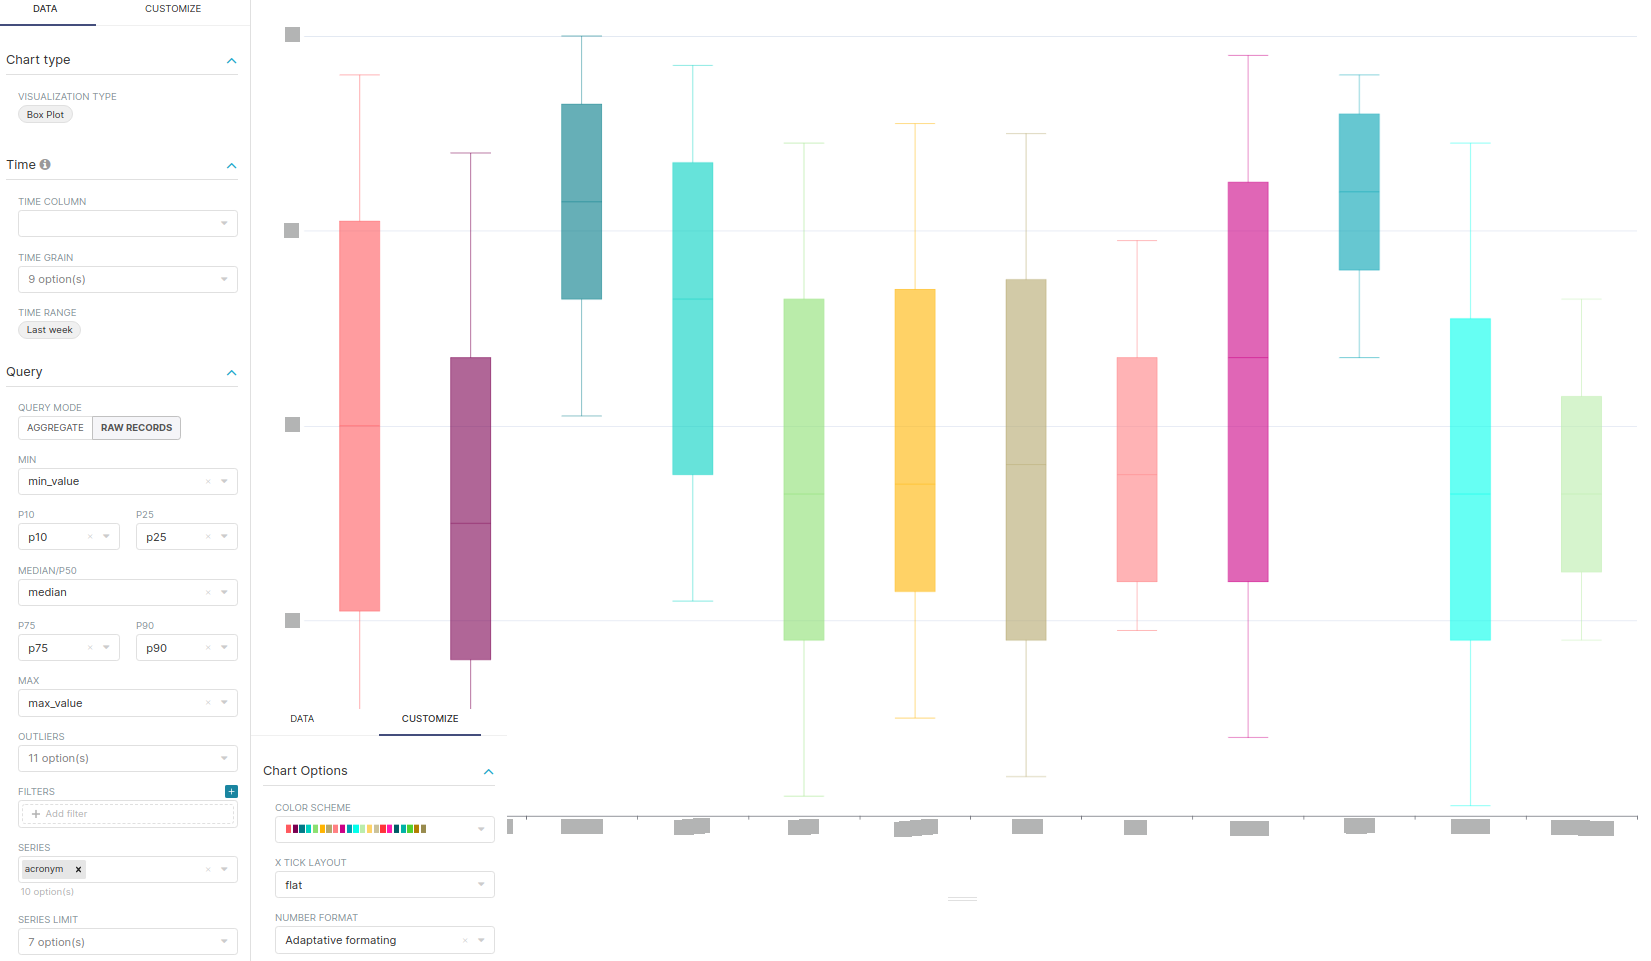
\includegraphics{images/11-network-dashboard/03-demographics/06-dist-age-at-fist-obs-period.png}

\hypertarget{year-of-birth}{%
\subsubsection*{Year of Birth}\label{year-of-birth}}
\addcontentsline{toc}{subsubsection}{Year of Birth}

Dataset: Materialized View \href{materialized-views-1.html\#year_of_birth}{year\_of\_birth}

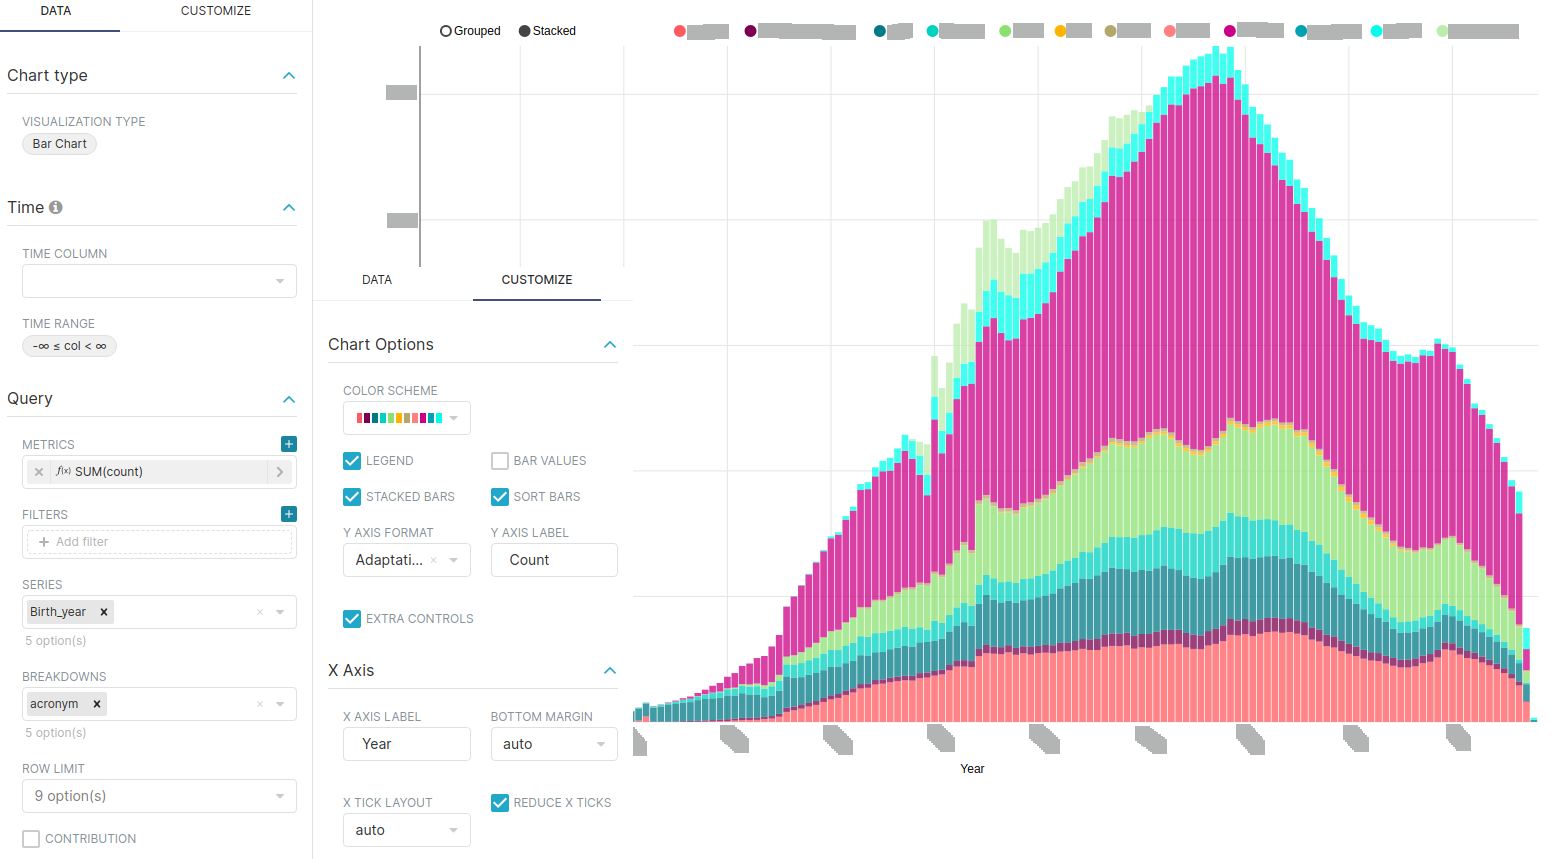
\includegraphics{images/11-network-dashboard/03-demographics/07-year-of-birth.png}

\hypertarget{data-domains-tab}{%
\subsection*{Data Domains Tab}\label{data-domains-tab}}
\addcontentsline{toc}{subsection}{Data Domains Tab}

\hypertarget{average-number-of-records-per-person}{%
\subsubsection*{Average number of records per person}\label{average-number-of-records-per-person}}
\addcontentsline{toc}{subsubsection}{Average number of records per person}

Dataset: Materialized View \href{materialized-views-1.html\#avg_num_of_records_per_person}{avg\_num\_of\_records\_per\_person}

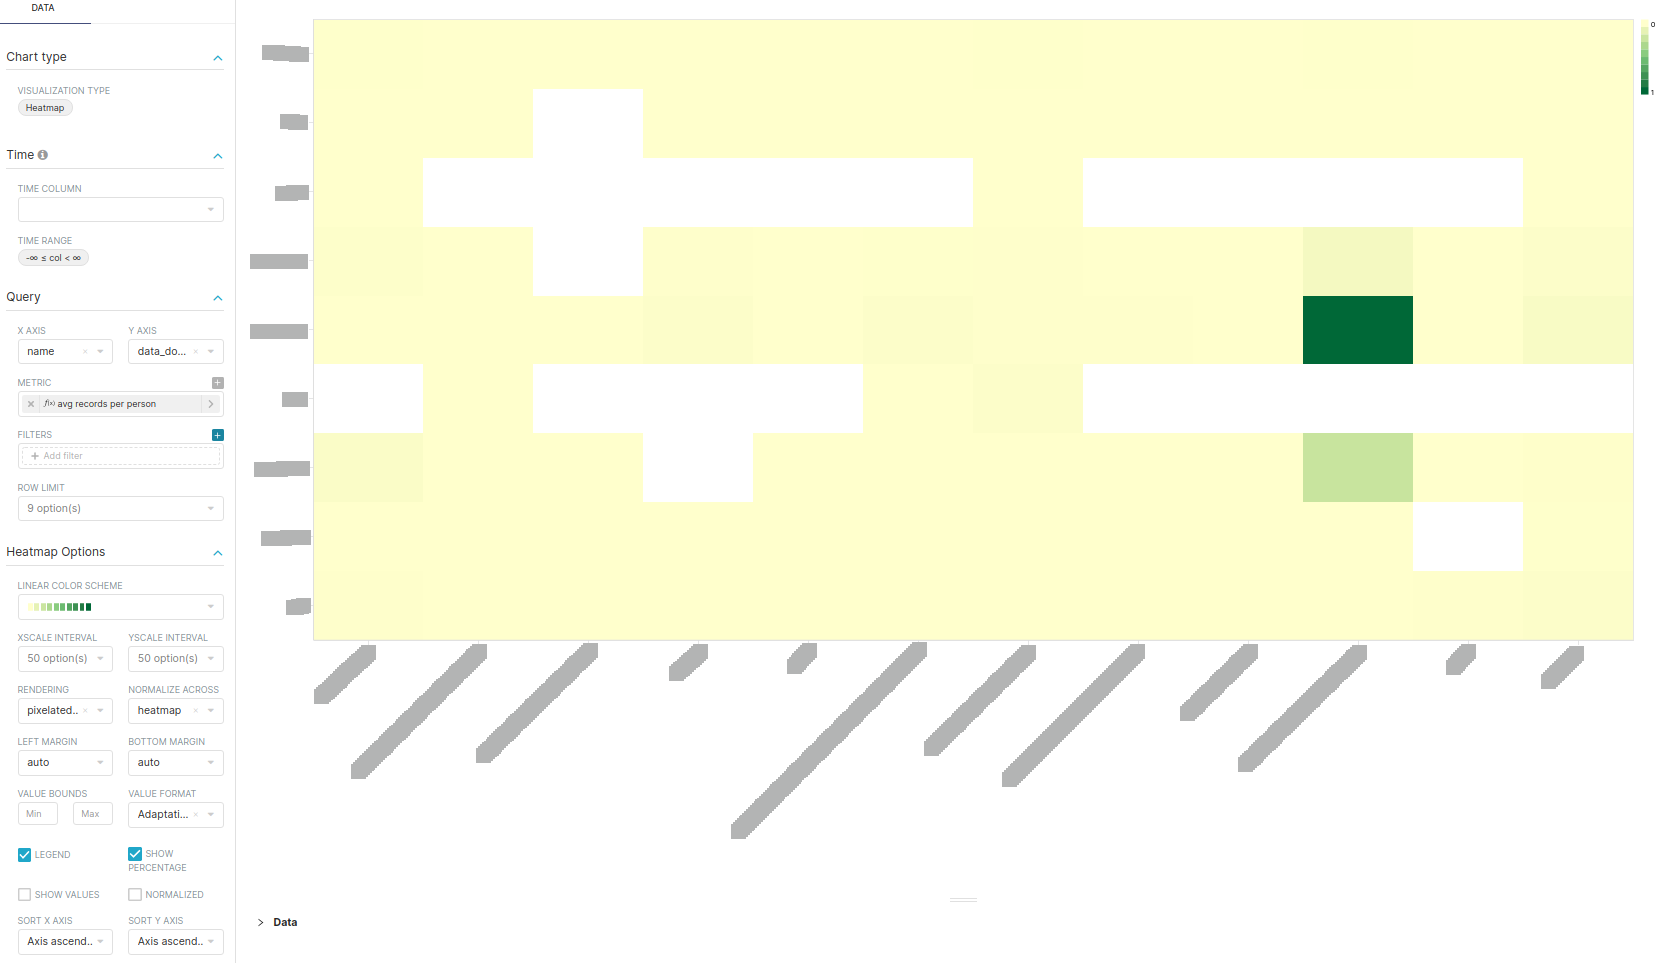
\includegraphics{images/11-network-dashboard/04-data-domains/01-avg-num-recs-per-person.png}

\hypertarget{total-number-of-records}{%
\subsubsection*{Total number of records}\label{total-number-of-records}}
\addcontentsline{toc}{subsubsection}{Total number of records}

Dataset: Materialized View \href{materialized-views-1.html\#data_domain_total_num_of_records}{data\_domain\_total\_num\_of\_records}

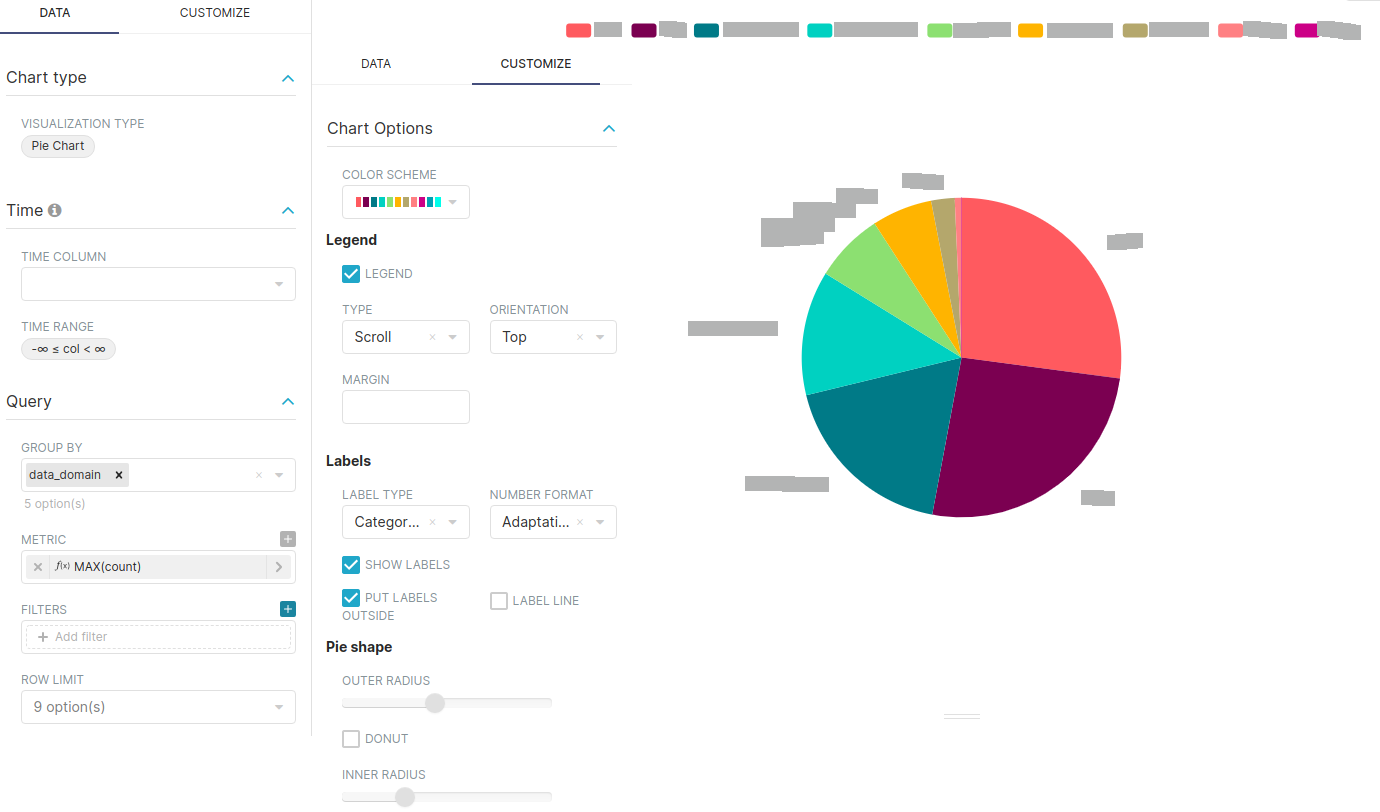
\includegraphics{images/11-network-dashboard/04-data-domains/02-total-num-of-rec.png}

\hypertarget{number-of-distinct-visit-occurrence-concepts-per-person}{%
\subsubsection*{Number of distinct visit occurrence concepts per person}\label{number-of-distinct-visit-occurrence-concepts-per-person}}
\addcontentsline{toc}{subsubsection}{Number of distinct visit occurrence concepts per person}

Dataset: Materialized View \href{materialized-views-1.html\#number_of_distinct_per_person}{number\_of\_distinct\_per\_person}

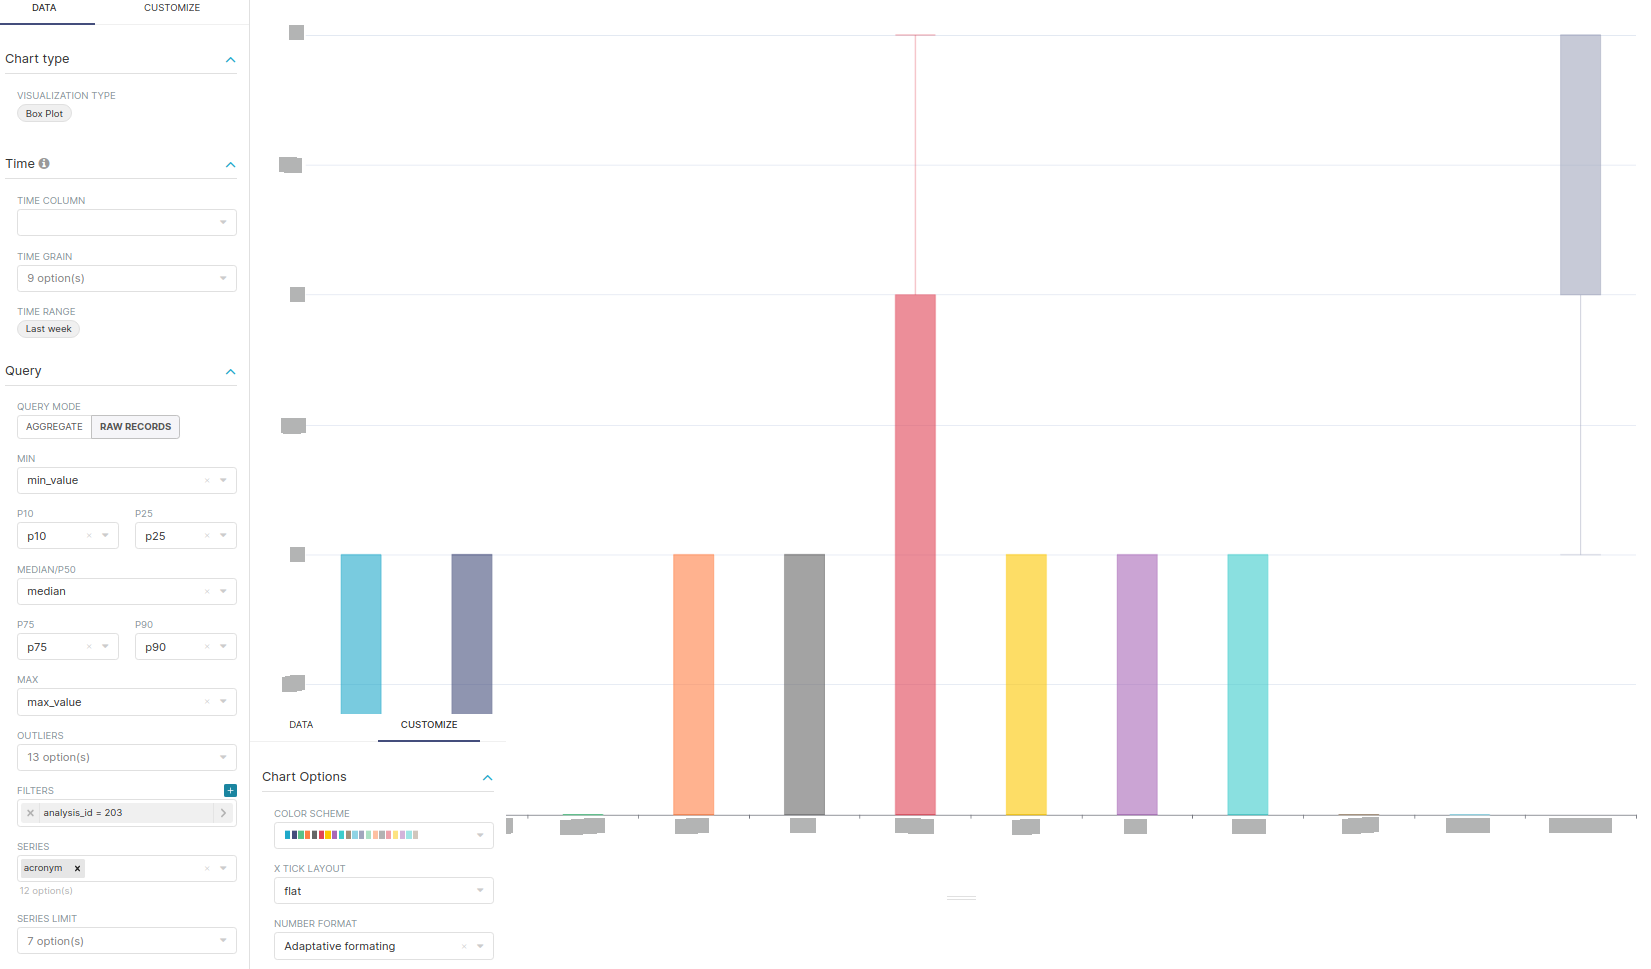
\includegraphics{images/11-network-dashboard/04-data-domains/03-num-distinct-visit-occurr-concepts-pperson.png}

\hypertarget{number-of-distinct-condition-occurrence-concepts-per-person}{%
\subsubsection*{Number of distinct condition occurrence concepts per person}\label{number-of-distinct-condition-occurrence-concepts-per-person}}
\addcontentsline{toc}{subsubsection}{Number of distinct condition occurrence concepts per person}

Dataset: Materialized View \href{materialized-views-1.html\#number_of_distinct_per_person}{number\_of\_distinct\_per\_person}

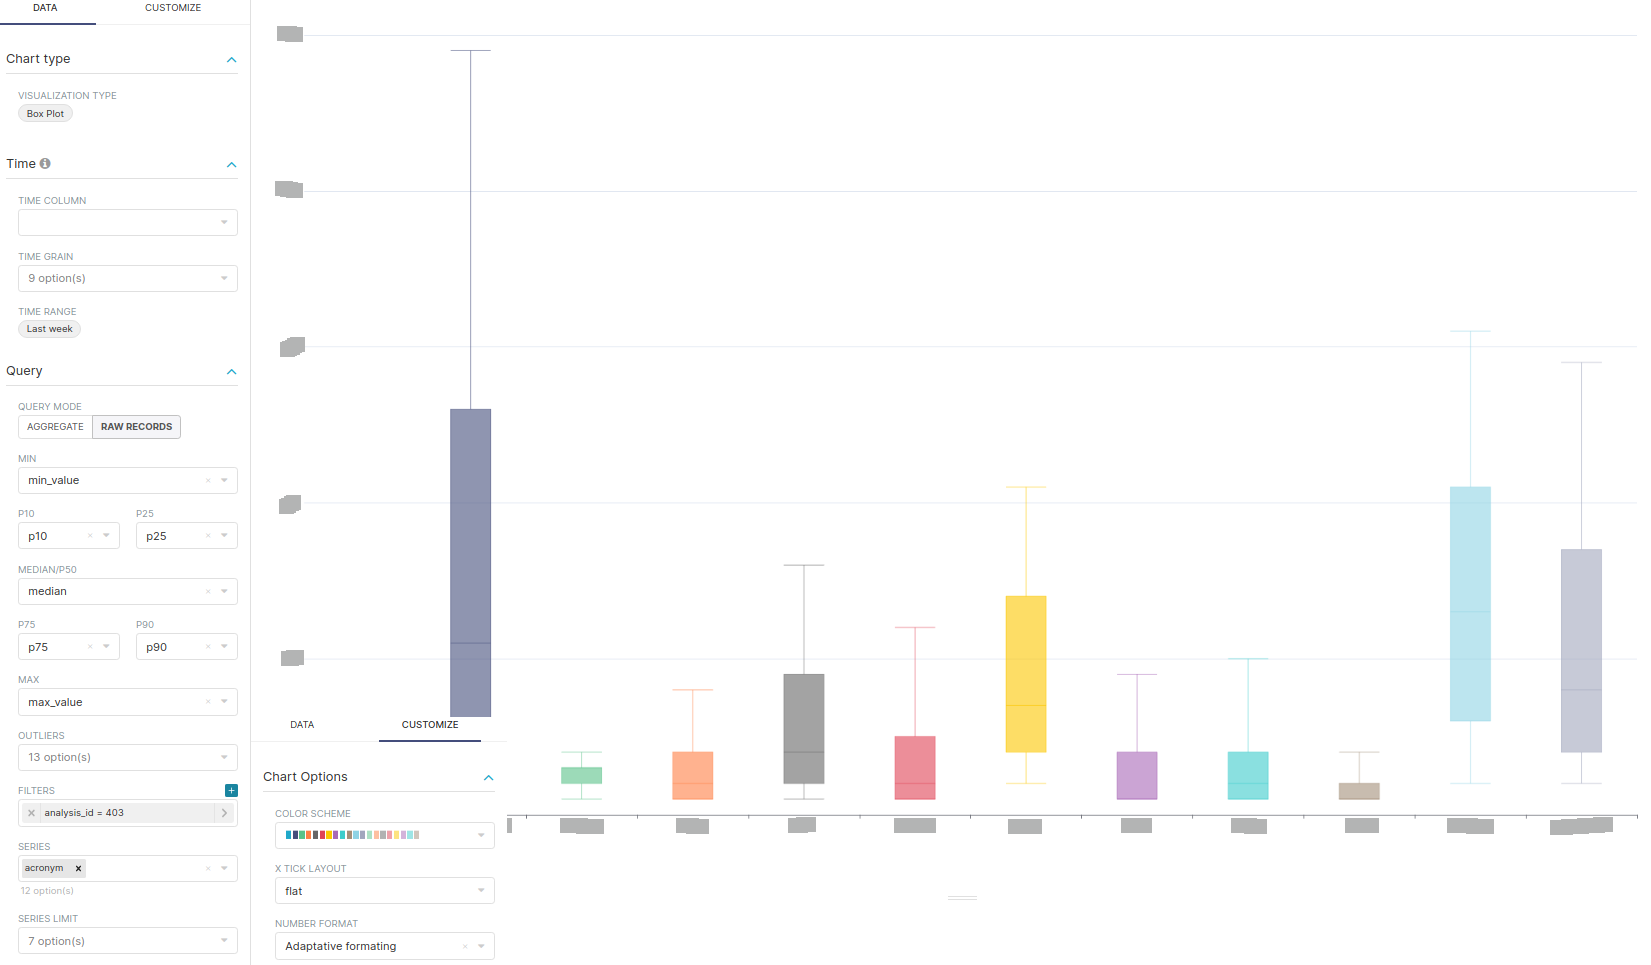
\includegraphics{images/11-network-dashboard/04-data-domains/04-num-distinct-cond-occur-concepts-pperson.png}

\hypertarget{number-of-distinct-procedure-occurrence-concepts-per-person}{%
\subsubsection*{Number of distinct procedure occurrence concepts per person}\label{number-of-distinct-procedure-occurrence-concepts-per-person}}
\addcontentsline{toc}{subsubsection}{Number of distinct procedure occurrence concepts per person}

Dataset: Materialized View \href{materialized-views-1.html\#number_of_distinct_per_person}{number\_of\_distinct\_per\_person}

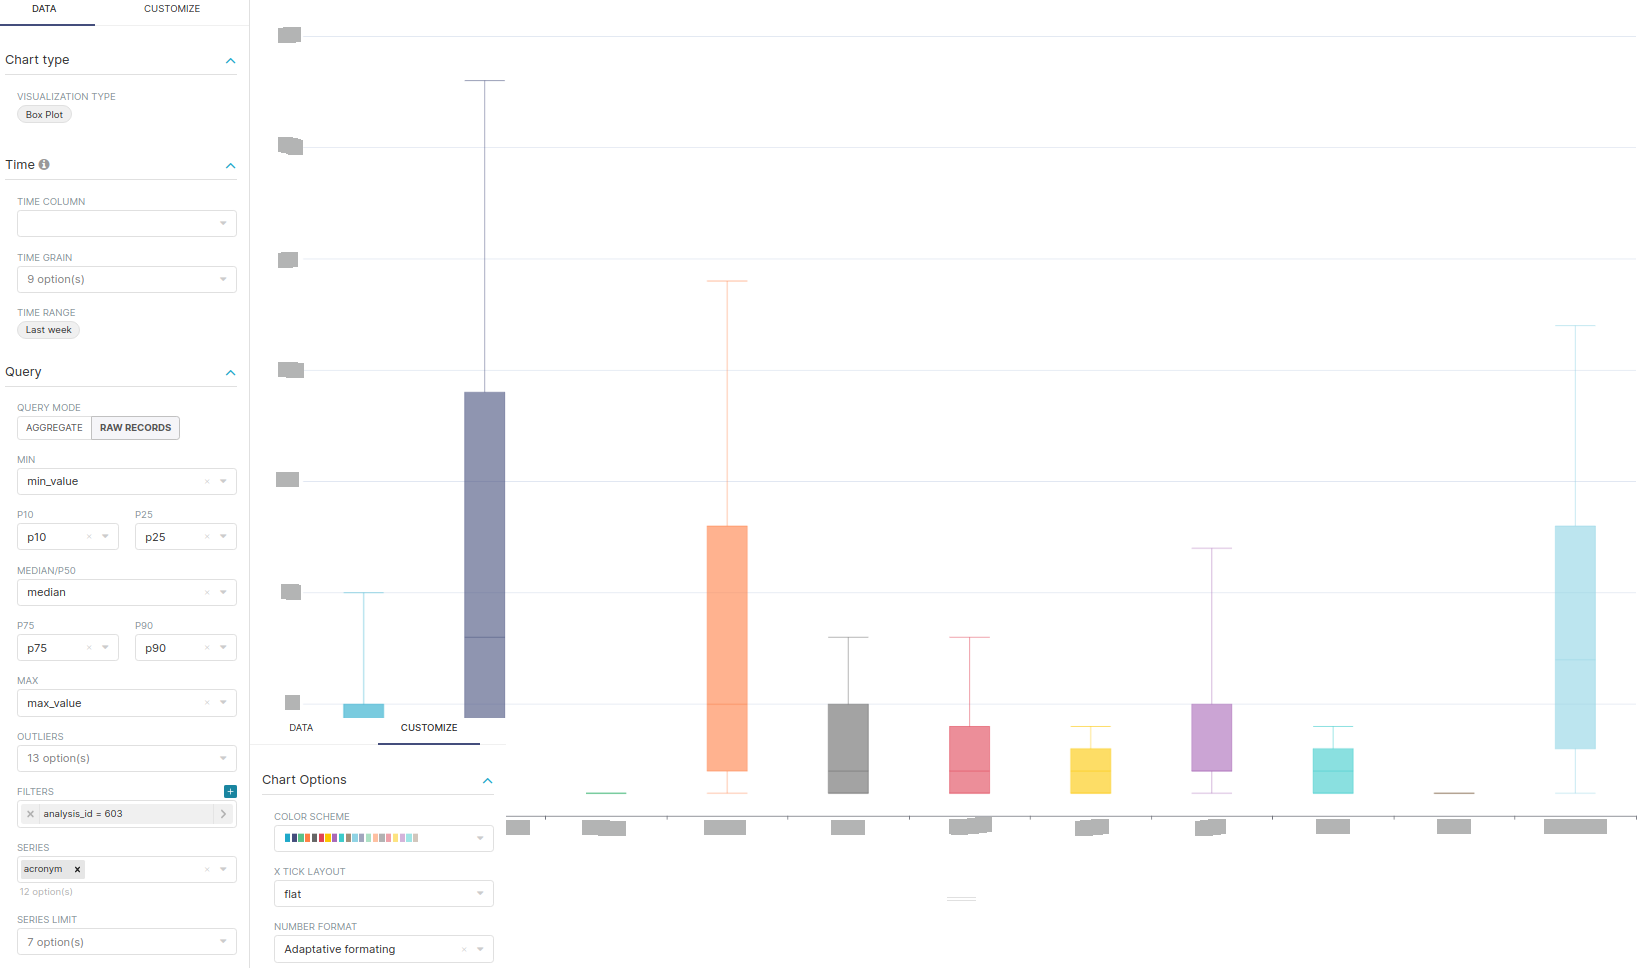
\includegraphics{images/11-network-dashboard/04-data-domains/05-num-distinct-proced-occur-concepts-pperson.png}

\hypertarget{number-of-distinct-drug-exposure-concepts-per-person}{%
\subsubsection*{Number of distinct drug exposure concepts per person}\label{number-of-distinct-drug-exposure-concepts-per-person}}
\addcontentsline{toc}{subsubsection}{Number of distinct drug exposure concepts per person}

Dataset: Materialized View \href{materialized-views-1.html\#number_of_distinct_per_person}{number\_of\_distinct\_per\_person}

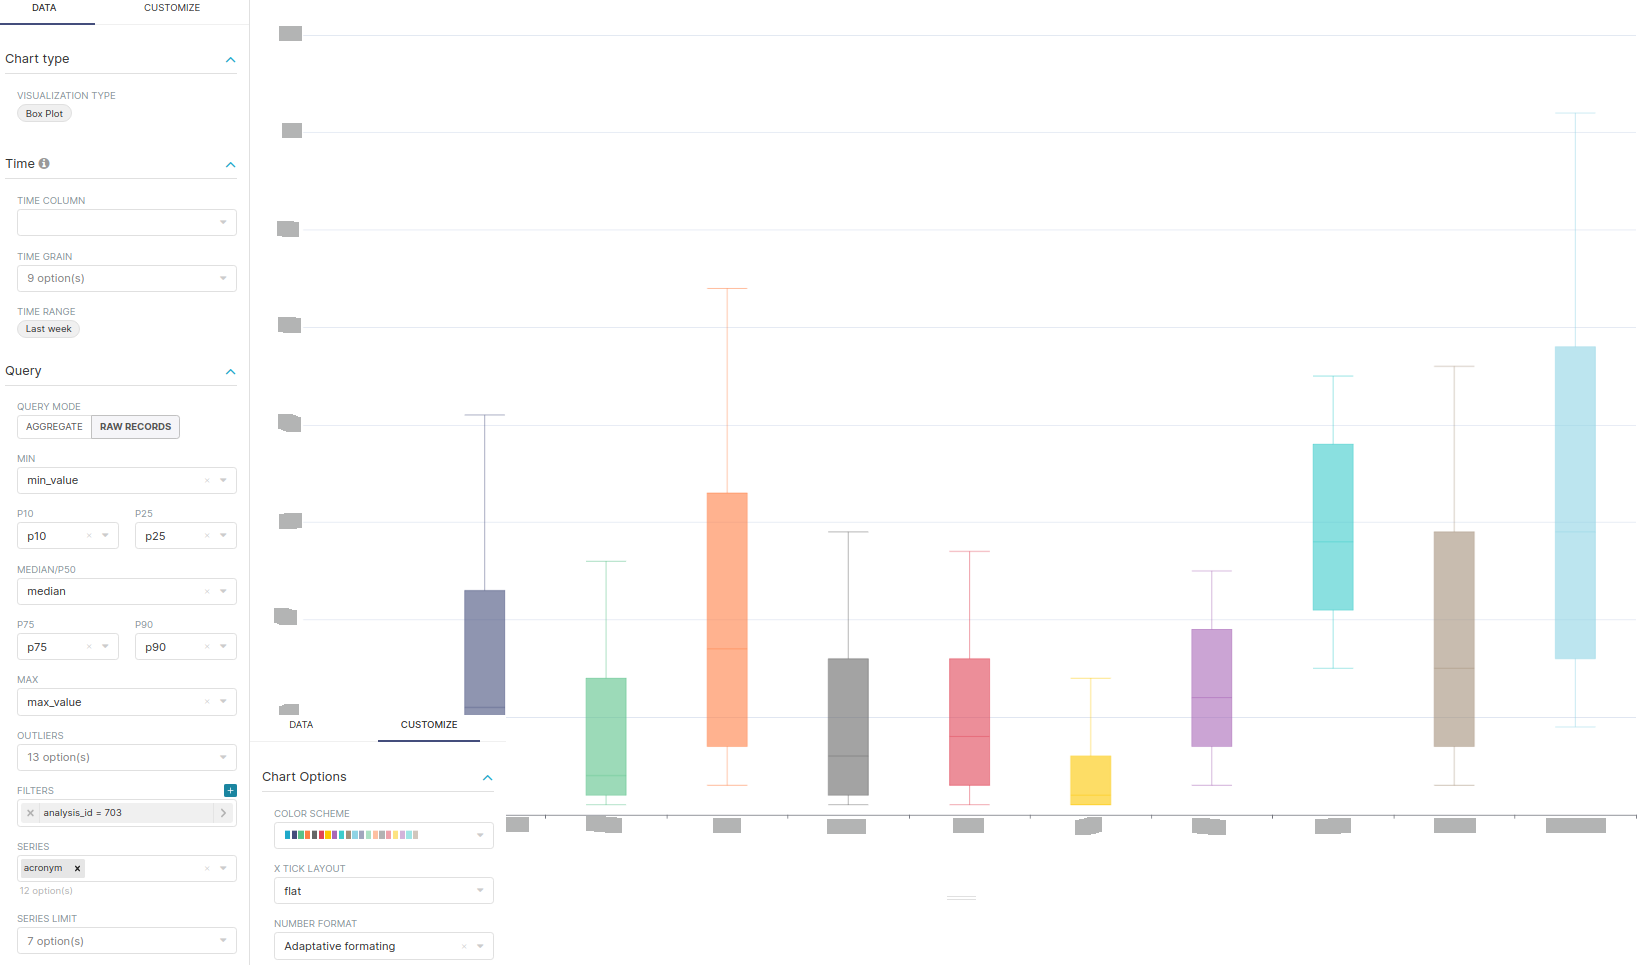
\includegraphics{images/11-network-dashboard/04-data-domains/06-num-distinct-drug-occur-concepts-pperson.png}

\hypertarget{number-of-distinct-observation-occurrence-concepts-per-person}{%
\subsubsection*{Number of distinct observation occurrence concepts per person}\label{number-of-distinct-observation-occurrence-concepts-per-person}}
\addcontentsline{toc}{subsubsection}{Number of distinct observation occurrence concepts per person}

Dataset: Materialized View \href{materialized-views-1.html\#number_of_distinct_per_person}{number\_of\_distinct\_per\_person}

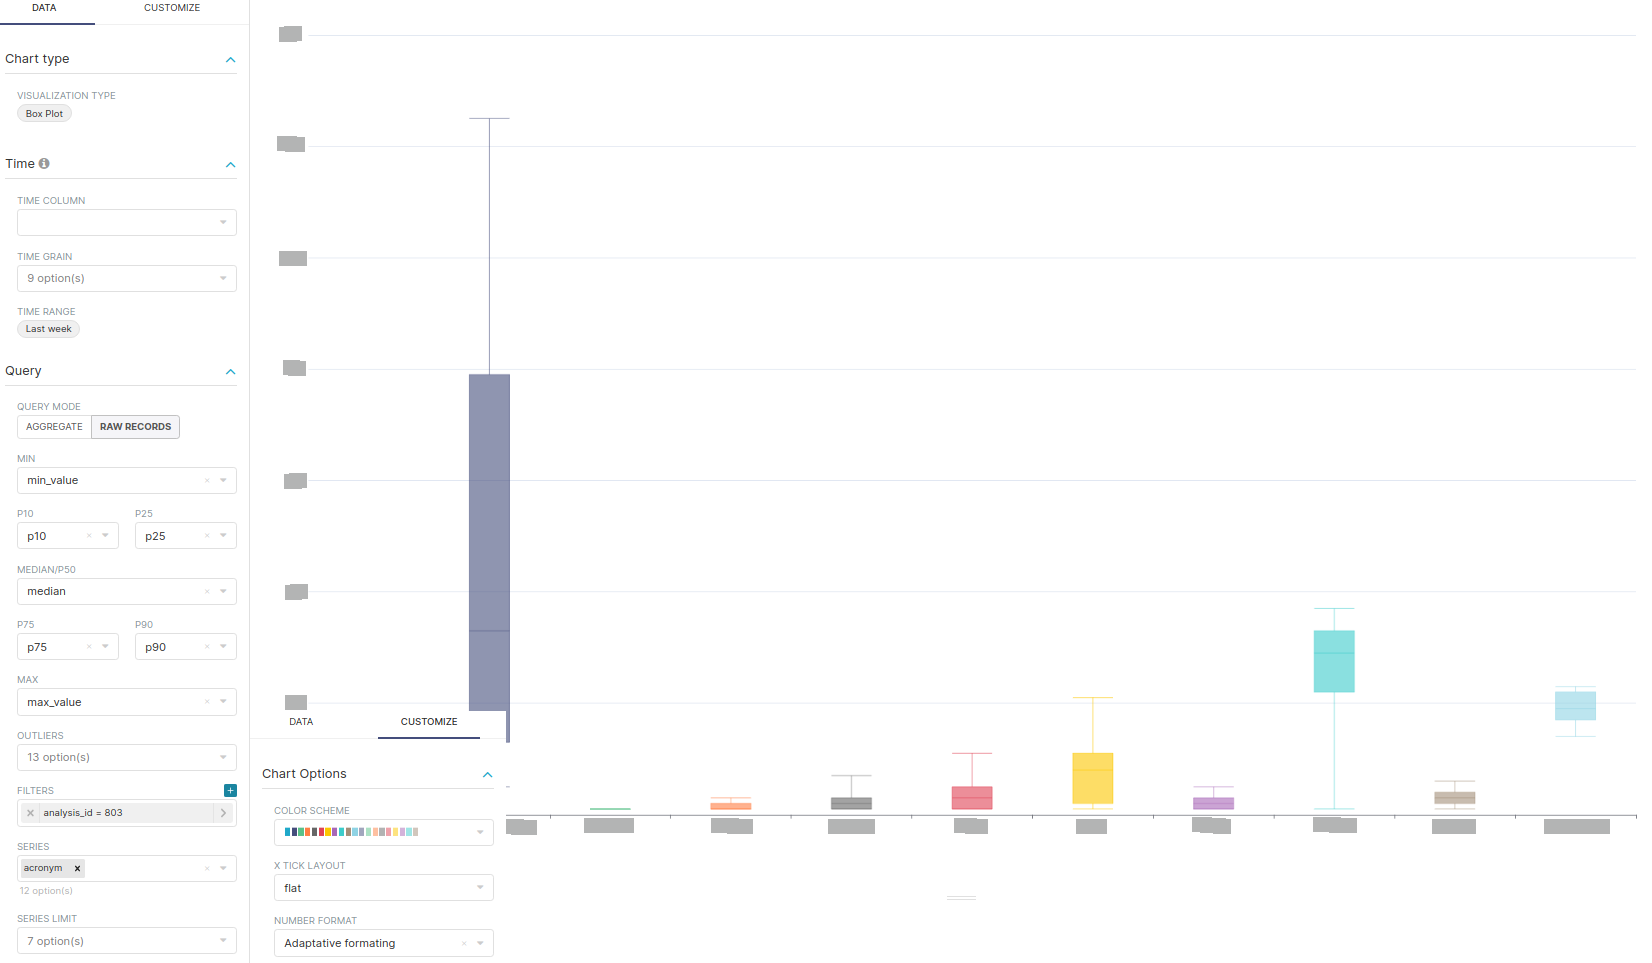
\includegraphics{images/11-network-dashboard/04-data-domains/07-num-distinct-observ-occur-concepts-pperson.png}

\hypertarget{number-of-distinct-mesurement-occurrence-concepts-per-person}{%
\subsubsection*{Number of distinct mesurement occurrence concepts per person}\label{number-of-distinct-mesurement-occurrence-concepts-per-person}}
\addcontentsline{toc}{subsubsection}{Number of distinct mesurement occurrence concepts per person}

Dataset: Materialized View \href{materialized-views-1.html\#number_of_distinct_per_person}{number\_of\_distinct\_per\_person}

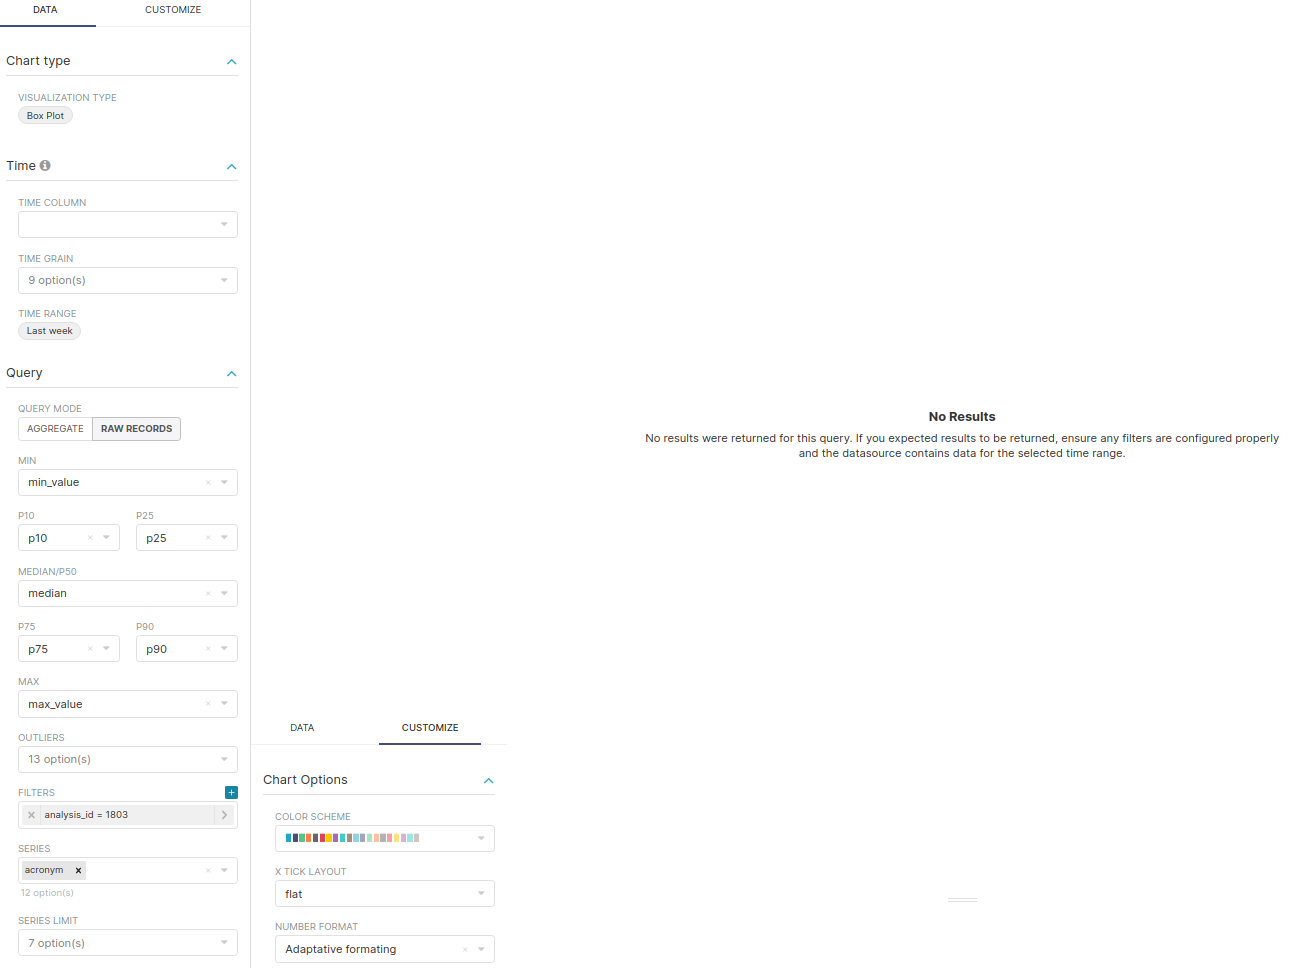
\includegraphics{images/11-network-dashboard/04-data-domains/08-num-distinct-mesur-occur-concepts-pperson.png}

\hypertarget{data-provenance-tab}{%
\subsection*{Data Provenance Tab}\label{data-provenance-tab}}
\addcontentsline{toc}{subsection}{Data Provenance Tab}

Dataset: Materialized View \href{materialized-views-1.html\#data_provenance}{data\_provenance}

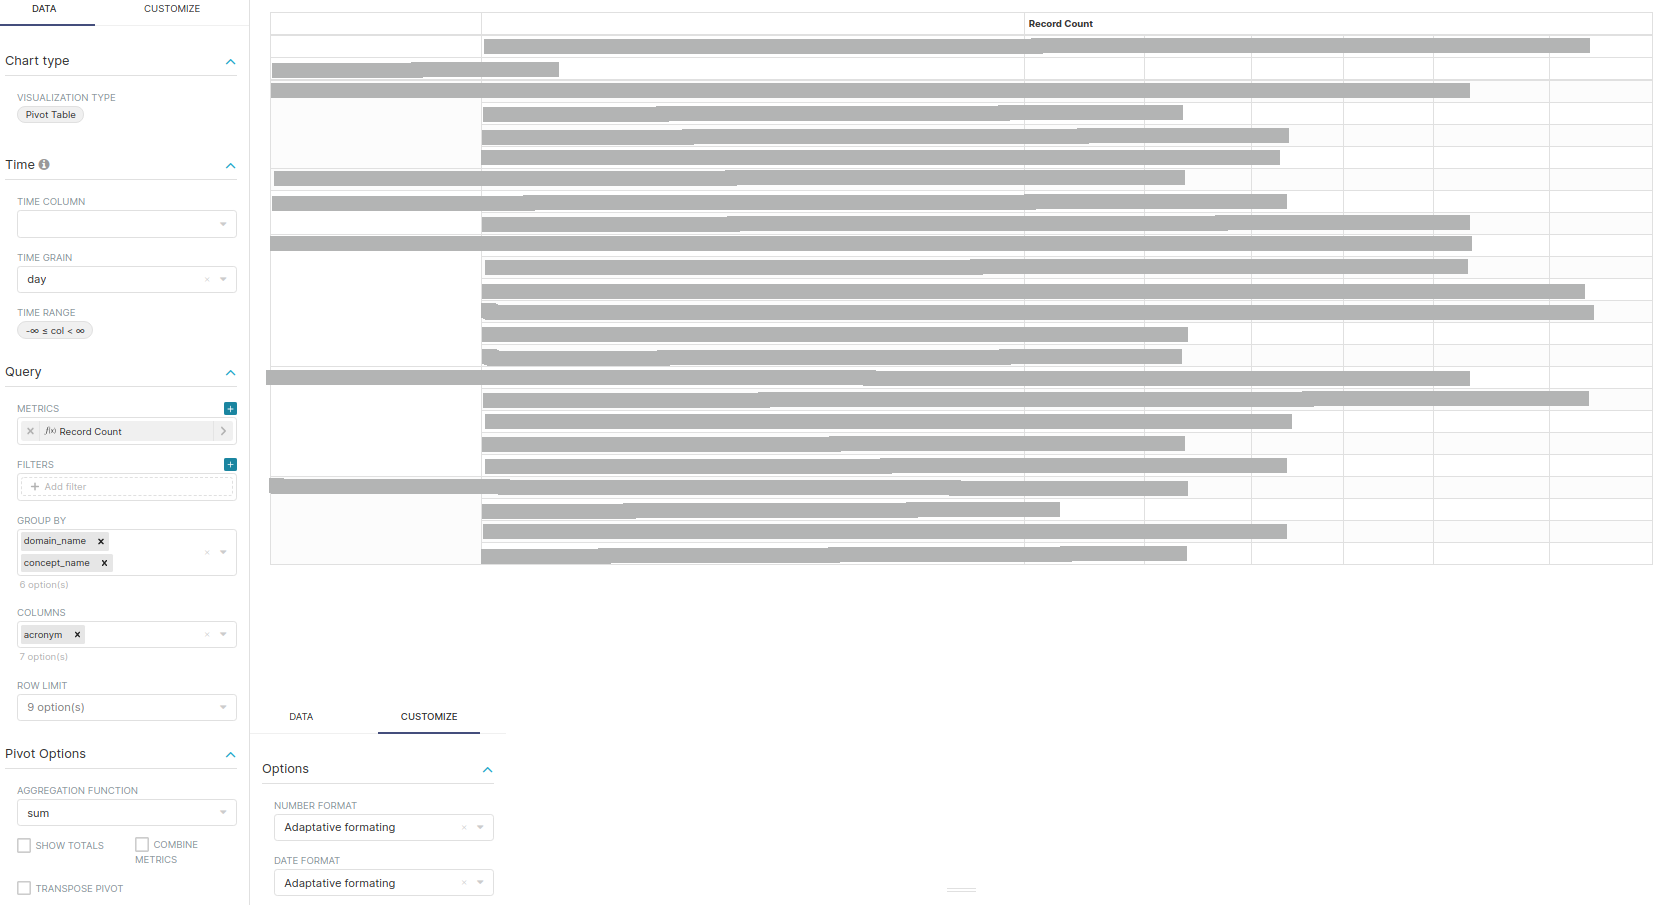
\includegraphics{images/11-network-dashboard/05-visit-type-pivot.png}

\hypertarget{observation-period-tab}{%
\subsection*{Observation Period Tab}\label{observation-period-tab}}
\addcontentsline{toc}{subsection}{Observation Period Tab}

\hypertarget{number-of-patitents-in-observation-period}{%
\subsubsection*{Number of Patitents in Observation Period}\label{number-of-patitents-in-observation-period}}
\addcontentsline{toc}{subsubsection}{Number of Patitents in Observation Period}

Dataset: Materialized View \href{materialized-views-1.html\#num_of_patients_in_observation_period}{num\_of\_patients\_in\_observation\_period}

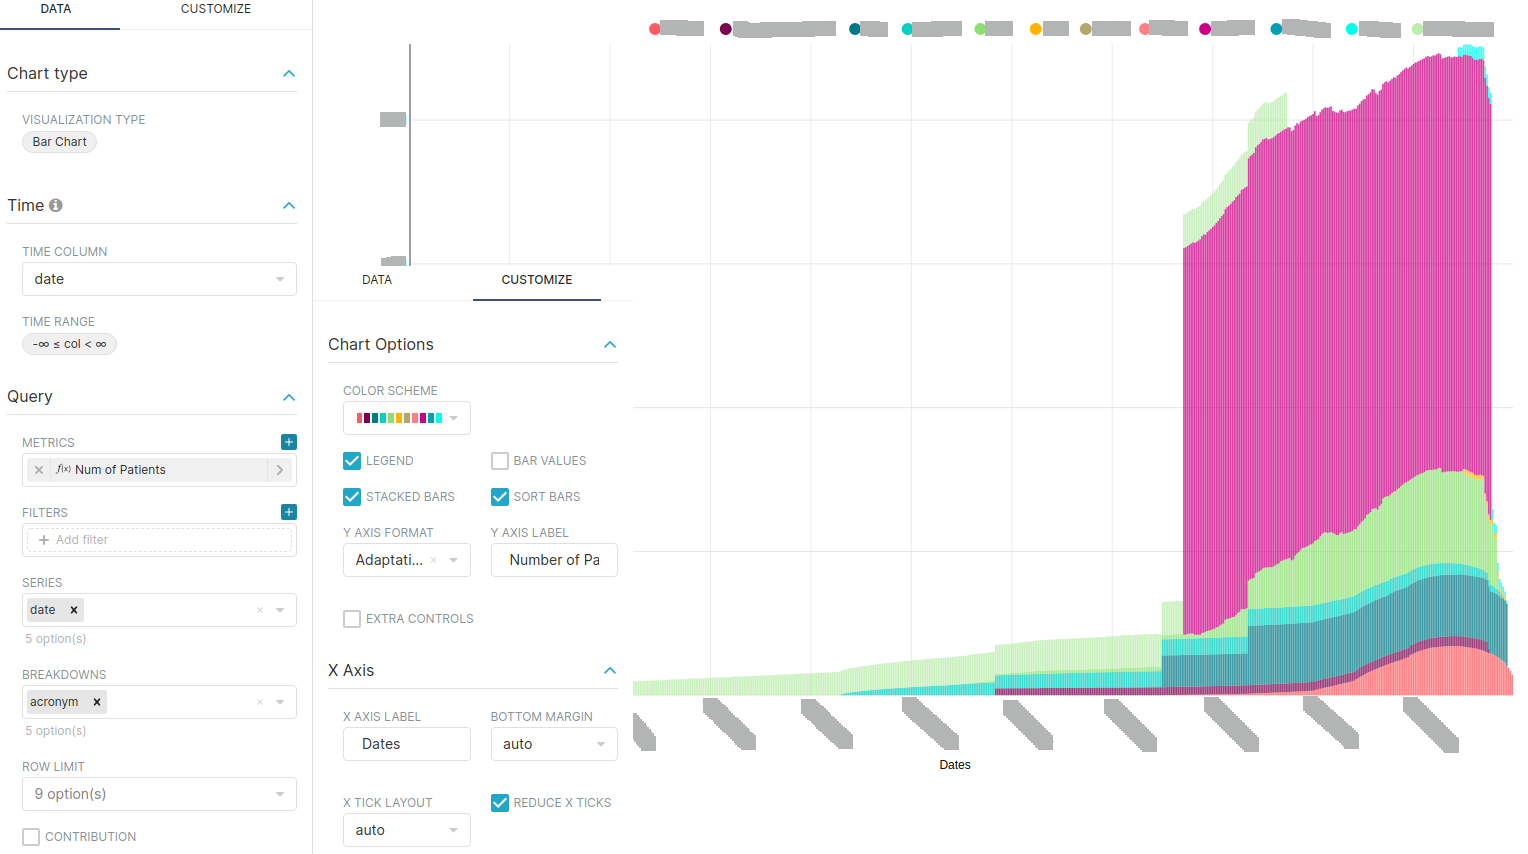
\includegraphics{images/11-network-dashboard/06-observation-period/01-num-patients-in-ober-period.png}

\hypertarget{cumulative-observation-period}{%
\subsubsection*{Cumulative Observation Period}\label{cumulative-observation-period}}
\addcontentsline{toc}{subsubsection}{Cumulative Observation Period}

Dataset: Materialized View \href{materialized-views-1.html\#cumulative_observation_time}{cumulative\_observation\_time}

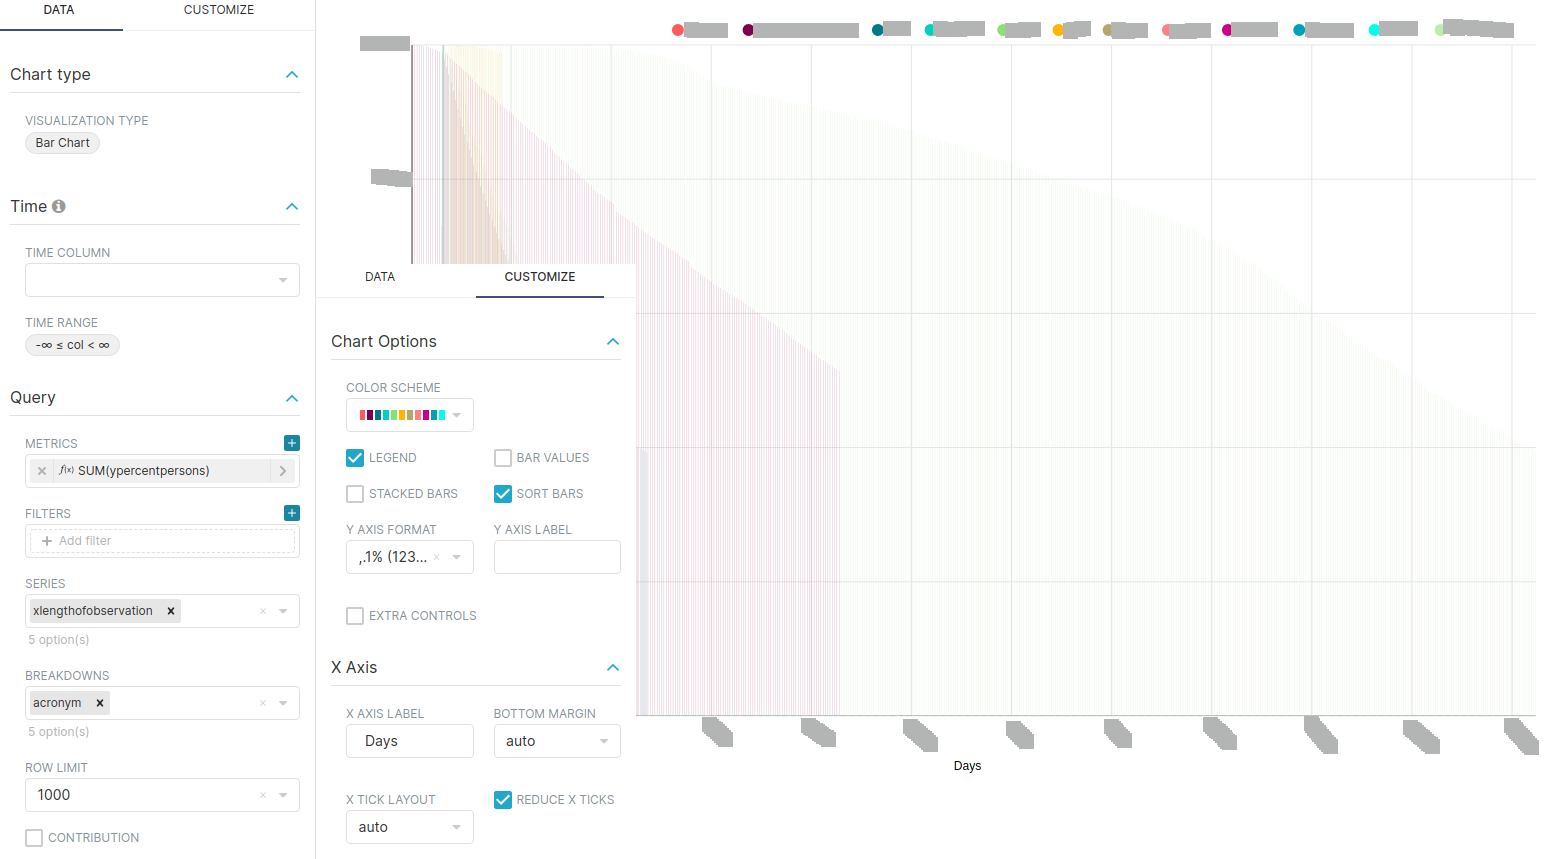
\includegraphics{images/11-network-dashboard/06-observation-period/02-cumulative-oberv-time.png}

\hypertarget{number-of-observation-periods}{%
\subsubsection*{Number of Observation Periods}\label{number-of-observation-periods}}
\addcontentsline{toc}{subsubsection}{Number of Observation Periods}

Dataset: Materialized View \href{materialized-views-1.html\#number_of_observation_periods}{number\_of\_observation\_periods}

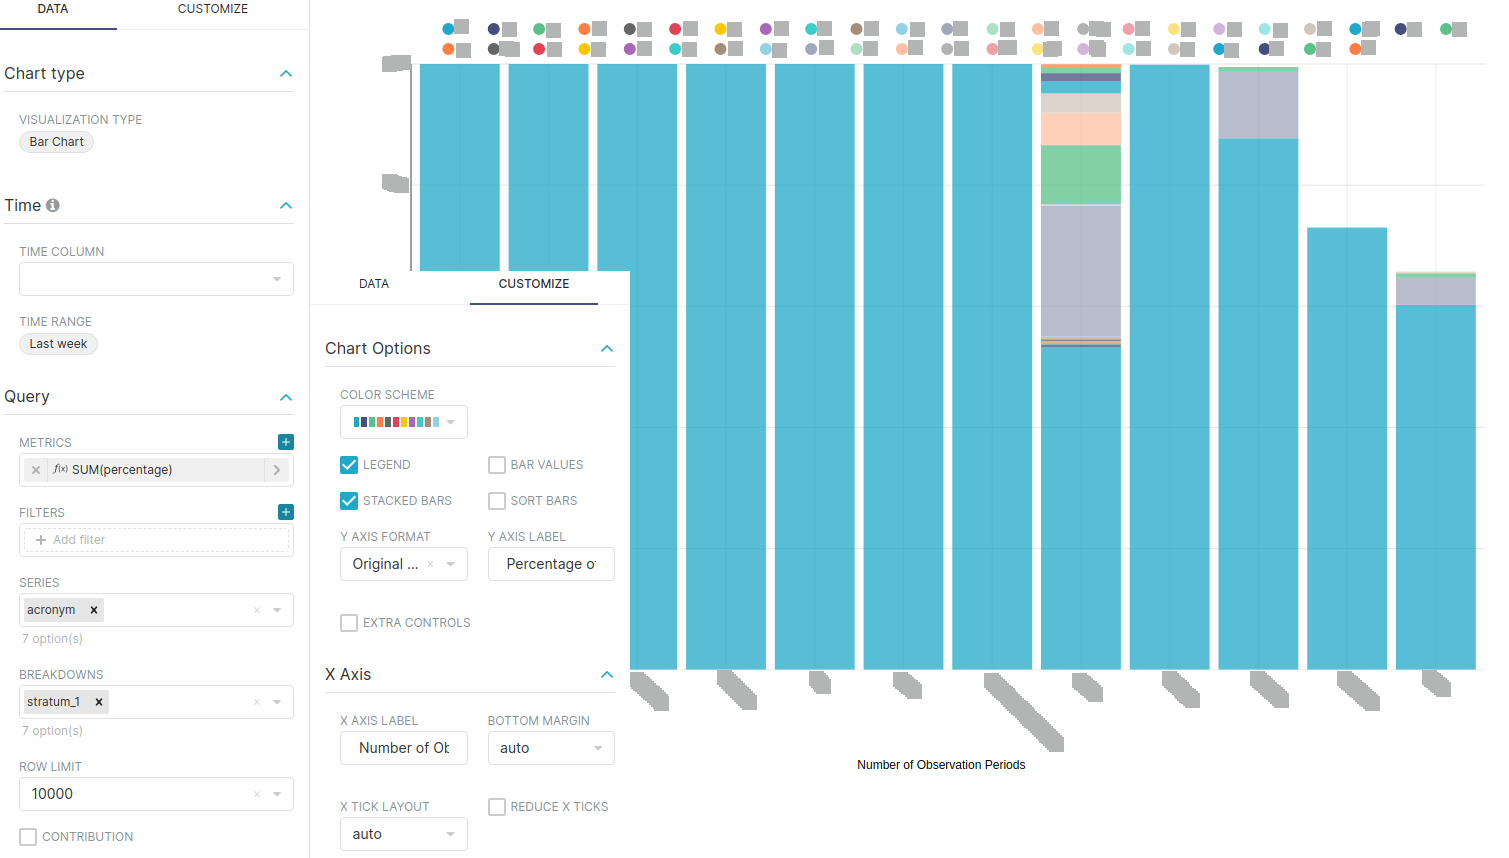
\includegraphics{images/11-network-dashboard/06-observation-period/03-num-observ-periods.png}

\hypertarget{length-of-observation-days-of-first-observation-period}{%
\subsubsection*{Length of observation (days) of first observation period}\label{length-of-observation-days-of-first-observation-period}}
\addcontentsline{toc}{subsubsection}{Length of observation (days) of first observation period}

Dataset: Materialized View \href{materialized-views-1.html\#length_of_observation_of_first_observation_period}{length\_of\_observation\_of\_first\_observation\_period}

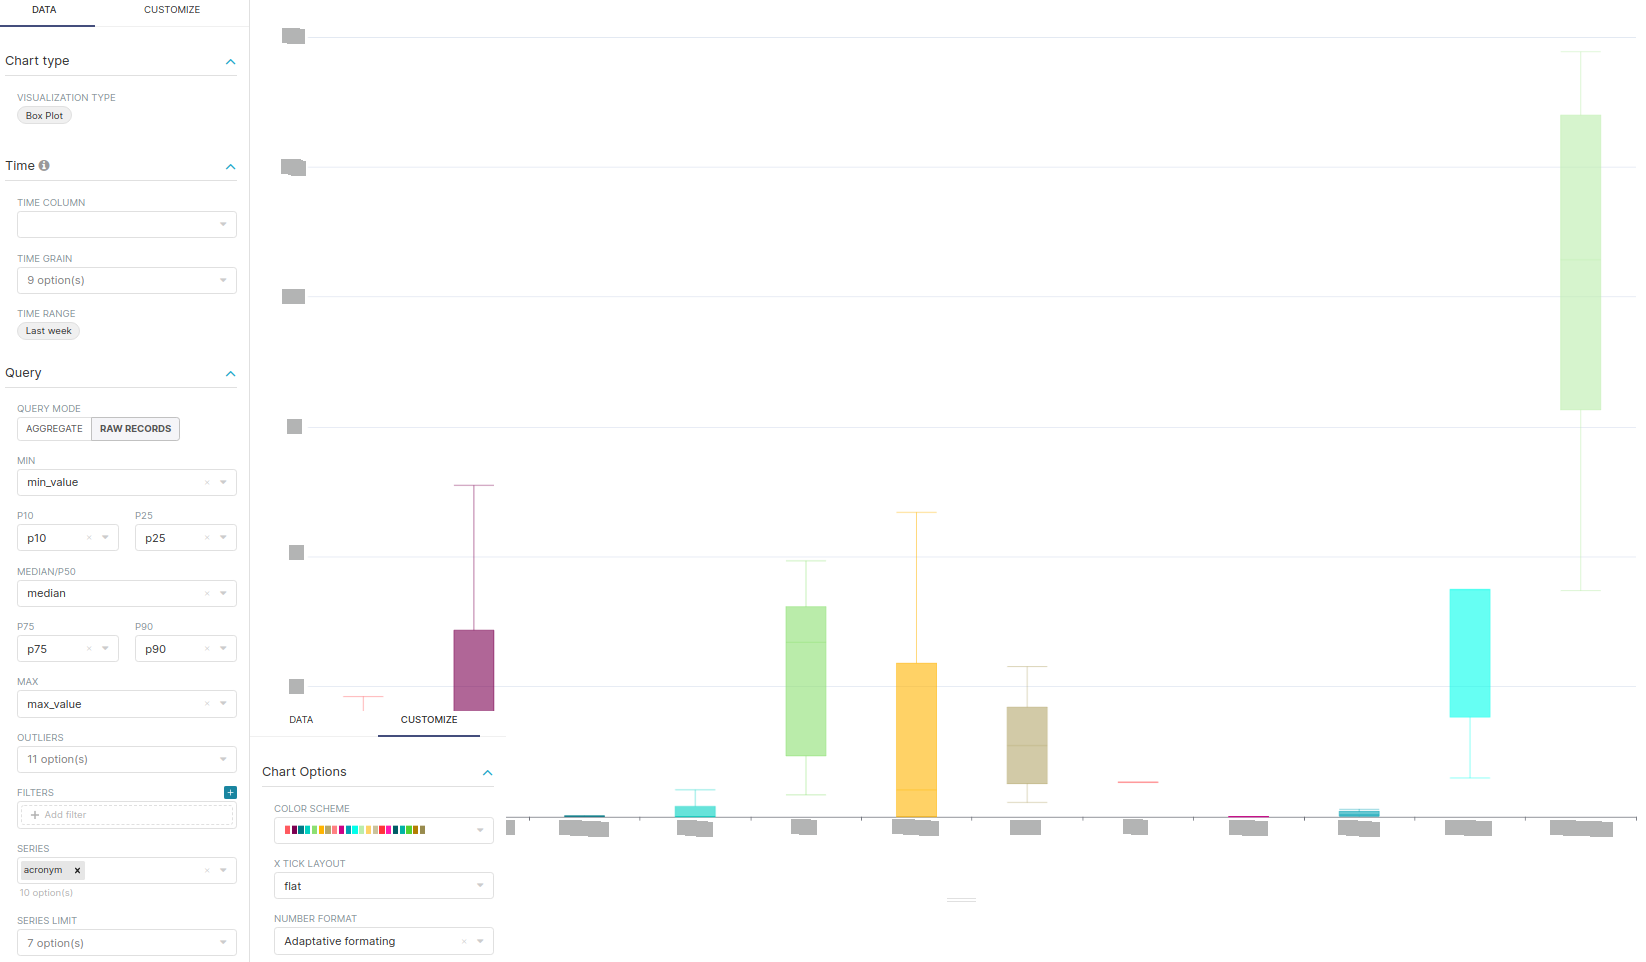
\includegraphics{images/11-network-dashboard/06-observation-period/04-len-observ-days-first-observ-period.png}

\hypertarget{visit-tab}{%
\subsection*{Visit Tab}\label{visit-tab}}
\addcontentsline{toc}{subsection}{Visit Tab}

\hypertarget{visit-type-graph}{%
\subsubsection*{Visit Type Graph}\label{visit-type-graph}}
\addcontentsline{toc}{subsubsection}{Visit Type Graph}

Dataset: Materialized View \href{materialized-views-1.html\#visit_type_bar_chart}{visit\_type\_bar\_chart}

\includegraphics{images/11-network-dashboard/07-visit/01-visit-type-graph.png}

\hypertarget{visit-type}{%
\subsubsection*{Visit Type}\label{visit-type}}
\addcontentsline{toc}{subsubsection}{Visit Type}

Dataset: Materialized View \href{materialized-views-1.html\#visit_type_table}{visit\_type\_table}

\includegraphics{images/11-network-dashboard/07-visit/02-visit-type.png}

\hypertarget{concept-browser-tab}{%
\subsection*{Concept Browser Tab}\label{concept-browser-tab}}
\addcontentsline{toc}{subsection}{Concept Browser Tab}

\hypertarget{domain-filter}{%
\subsubsection*{Domain Filter}\label{domain-filter}}
\addcontentsline{toc}{subsubsection}{Domain Filter}

Dataset: Materialized View \href{materialized-views-1.html\#domain_filter}{domain\_filter}

\includegraphics{images/11-network-dashboard/08-concept-browser/01-domain-filter.png}

\hypertarget{concept-browser}{%
\subsubsection*{Concept Browser}\label{concept-browser}}
\addcontentsline{toc}{subsubsection}{Concept Browser}

Dataset: Materialized View \href{materialized-views-1.html\#concept_browser_table3}{concept\_browser\_table3}

\includegraphics{images/11-network-dashboard/08-concept-browser/02-concept-browser.png}

\hypertarget{concept-network-coverage}{%
\subsubsection*{Concept Network Coverage}\label{concept-network-coverage}}
\addcontentsline{toc}{subsubsection}{Concept Network Coverage}

Dataset: Materialized View \href{materialized-views-1.html\#concept_coverage2}{concept\_coverage2}

\includegraphics{images/11-network-dashboard/08-concept-browser/03-concept-network-coverage.png}

\hypertarget{about-tab}{%
\subsection*{About Tab}\label{about-tab}}
\addcontentsline{toc}{subsection}{About Tab}

Markdown dashboard components

\includegraphics{images/11-network-dashboard/09-about.png}

\hypertarget{database-level-dashboard}{%
\section{Database-Level Dashboard}\label{database-level-dashboard}}

This dashboard is an exact copy of the \protect\hyperlink{PerDatabaseDashboard}{Network Dashboard} dashboard but several legends and fields
displayed on the original are hidden either through CSS or by changing some chart settings.
On the following sections we will only present the things to change on the original charts.

\hypertarget{label-colors-1}{%
\subsection*{Label Colors}\label{label-colors-1}}
\addcontentsline{toc}{subsection}{Label Colors}

In order to obtain the colors blue and rose in the chart representing the gender distribution,
add the following JSON entry to the JSON object of the \texttt{JSON\ Metadata} field on the edit dashboard page:

\begin{Shaded}
\begin{Highlighting}[]
\ErrorTok{"label\_colors":} \FunctionTok{\{}
    \DataTypeTok{"Male"}\FunctionTok{:} \StringTok{"\#3366FF"}\FunctionTok{,}
    \DataTypeTok{"Female"}\FunctionTok{:} \StringTok{"\#FF3399"}
\FunctionTok{\}}
\end{Highlighting}
\end{Shaded}

\hypertarget{css-1}{%
\subsection*{CSS}\label{css-1}}
\addcontentsline{toc}{subsection}{CSS}

To hide the dashboard header insert the following css code to the \texttt{CSS} field on the edit page:

\begin{Shaded}
\begin{Highlighting}[]
\CommentTok{/* hides the filter badges on right side of charts */}
\FunctionTok{.dashboard{-}filter{-}indicators{-}container}\NormalTok{ \{}
    \KeywordTok{display}\NormalTok{: }\DecValTok{none}\OperatorTok{;}
\NormalTok{\}}

\CommentTok{/* hides the acronym filter */}
\FunctionTok{.grid{-}content} \OperatorTok{\textgreater{}} \FunctionTok{.dragdroppable.dragdroppable{-}row} \OperatorTok{\textgreater{}} \FunctionTok{.with{-}popover{-}menu}\NormalTok{ \{}
    \KeywordTok{display}\NormalTok{: }\DecValTok{none}\OperatorTok{;}
\NormalTok{\}}

\CommentTok{/*}
\CommentTok{ * }\AlertTok{WARNING}\CommentTok{ panel 1 id hardcoded}
\CommentTok{ * Hides the X Axis Label of the heatmap on the Data Domains tab}
\CommentTok{ */}
\PreprocessorTok{\#TABS{-}nlIU6H5mcT{-}pane{-}1}\NormalTok{ g}\FunctionTok{.x.axis} \OperatorTok{\textgreater{}}\NormalTok{ g}\FunctionTok{.tick}\NormalTok{ text \{}
    \KeywordTok{display}\NormalTok{: }\DecValTok{none}\OperatorTok{;}
\NormalTok{\}}

\CommentTok{/*}
\CommentTok{ * }\AlertTok{WARNING}\CommentTok{ panel 2 id hardcoded}
\CommentTok{ * Hides the X Axis Labels of the bar charts on the Data Provenance tab}
\CommentTok{ */}
\PreprocessorTok{\#TABS{-}nlIU6H5mcT{-}pane{-}2}\NormalTok{ g}\FunctionTok{.nv{-}x.nv{-}axis.nvd3{-}svg} \OperatorTok{\textgreater{}}\NormalTok{ g}\FunctionTok{.nvd3.nv{-}wrap.nv{-}axis} \OperatorTok{\textgreater{}}\NormalTok{ g }\OperatorTok{\textgreater{}}\NormalTok{ g}\FunctionTok{.tick.zero} \OperatorTok{\textgreater{}}\NormalTok{ text \{}
    \KeywordTok{display}\NormalTok{: }\DecValTok{none}\OperatorTok{;}
\NormalTok{\}}
\end{Highlighting}
\end{Shaded}

With this every time you want to edit the dashboard layout you have to either comment the CSS inserted
or remove it so the ``Edit Dashboard'' button can show again.

\hypertarget{data-source-filter---hidden}{%
\subsection*{Data Source Filter - hidden}\label{data-source-filter---hidden}}
\addcontentsline{toc}{subsection}{Data Source Filter - hidden}

Dataset: \texttt{data\_source} table of the \texttt{achilles} database.

\textbf{For the filter to work the name of the fields to filter should match in all tables used on the charts of this dashboard.}

\includegraphics{images/12-database-level/01-acronym-filter.png}

\hypertarget{demographics-tab-1}{%
\subsection*{Demographics Tab}\label{demographics-tab-1}}
\addcontentsline{toc}{subsection}{Demographics Tab}

\hypertarget{number-of-patients-1}{%
\subsubsection*{Number of Patients}\label{number-of-patients-1}}
\addcontentsline{toc}{subsubsection}{Number of Patients}

No changes

\hypertarget{gender-table-1}{%
\subsubsection*{Gender Table}\label{gender-table-1}}
\addcontentsline{toc}{subsubsection}{Gender Table}

No changes

\hypertarget{gender-pie-1}{%
\subsubsection*{Gender Pie}\label{gender-pie-1}}
\addcontentsline{toc}{subsubsection}{Gender Pie}

No changes

\hypertarget{age-at-first-observation---bars}{%
\subsubsection*{Age at first observation - Bars}\label{age-at-first-observation---bars}}
\addcontentsline{toc}{subsubsection}{Age at first observation - Bars}

Remove legend.

\begin{itemize}
\tightlist
\item
  Customize Tab

  \begin{itemize}
  \tightlist
  \item
    Chart Options

    \begin{itemize}
    \tightlist
    \item
      Legend: off
    \end{itemize}
  \end{itemize}
\end{itemize}

\hypertarget{distribution-of-age-at-first-observation-period-1}{%
\subsubsection*{Distribution of age at first observation period}\label{distribution-of-age-at-first-observation-period-1}}
\addcontentsline{toc}{subsubsection}{Distribution of age at first observation period}

No changes

\hypertarget{year-of-birth-1}{%
\subsubsection*{Year of Birth}\label{year-of-birth-1}}
\addcontentsline{toc}{subsubsection}{Year of Birth}

Remove legend.

\begin{itemize}
\tightlist
\item
  Customize Tab

  \begin{itemize}
  \tightlist
  \item
    Chart Options

    \begin{itemize}
    \tightlist
    \item
      Legend: off
    \end{itemize}
  \end{itemize}
\end{itemize}

\hypertarget{data-domains-tab-1}{%
\subsection*{Data Domains Tab}\label{data-domains-tab-1}}
\addcontentsline{toc}{subsection}{Data Domains Tab}

\hypertarget{average-number-of-records-per-person-1}{%
\subsubsection*{Average number of records per person}\label{average-number-of-records-per-person-1}}
\addcontentsline{toc}{subsubsection}{Average number of records per person}

No changes

\hypertarget{total-number-of-records-1}{%
\subsubsection*{Total number of records}\label{total-number-of-records-1}}
\addcontentsline{toc}{subsubsection}{Total number of records}

No changes

\hypertarget{data-density-plot}{%
\subsubsection*{Data Density Plot}\label{data-density-plot}}
\addcontentsline{toc}{subsubsection}{Data Density Plot}

Dataset: Materialized View \href{materialized-views-1.html\#data_density}{data\_density}

\includegraphics{images/12-database-level/03-data-domains/03-data-density.png}

\hypertarget{records-per-person}{%
\subsubsection*{Records per person}\label{records-per-person}}
\addcontentsline{toc}{subsubsection}{Records per person}

Dataset: Materialized View \href{materialized-views-1.html\#records_per_person}{records\_per\_person}

\includegraphics{images/12-database-level/03-data-domains/04-records-per-person.png}

\hypertarget{concepts-per-person}{%
\subsubsection*{Concepts per person}\label{concepts-per-person}}
\addcontentsline{toc}{subsubsection}{Concepts per person}

Dataset: Materialized View \href{materialized-views-1.html\#number_of_distinct_per_person}{number\_of\_distinct\_per\_person}

\includegraphics{images/12-database-level/03-data-domains/05-concepts-pperson.png}

\hypertarget{data-provenance-tab-1}{%
\subsection*{Data Provenance Tab}\label{data-provenance-tab-1}}
\addcontentsline{toc}{subsection}{Data Provenance Tab}

\hypertarget{type-concepts}{%
\subsubsection*{Type Concepts}\label{type-concepts}}
\addcontentsline{toc}{subsubsection}{Type Concepts}

Dataset: Materialized View \href{materialized-views-1.html\#data_provenance}{data\_provenance}

\includegraphics{images/12-database-level/04-type-concepts.png}

\hypertarget{observation-period-tab-1}{%
\subsection*{Observation Period Tab}\label{observation-period-tab-1}}
\addcontentsline{toc}{subsection}{Observation Period Tab}

\hypertarget{number-of-patitents-in-observation-period-1}{%
\subsubsection*{Number of Patitents in Observation Period}\label{number-of-patitents-in-observation-period-1}}
\addcontentsline{toc}{subsubsection}{Number of Patitents in Observation Period}

Remove legend.

\begin{itemize}
\tightlist
\item
  Customize Tab

  \begin{itemize}
  \tightlist
  \item
    Chart Options

    \begin{itemize}
    \tightlist
    \item
      Legend: off
    \end{itemize}
  \end{itemize}
\end{itemize}

\hypertarget{length-of-observation-days-of-first-observation-period-1}{%
\subsubsection*{Length of observation (days) of first observation period}\label{length-of-observation-days-of-first-observation-period-1}}
\addcontentsline{toc}{subsubsection}{Length of observation (days) of first observation period}

No changes

\hypertarget{cumulative-observation-period-1}{%
\subsubsection*{Cumulative Observation Period}\label{cumulative-observation-period-1}}
\addcontentsline{toc}{subsubsection}{Cumulative Observation Period}

Remove legend.

\begin{itemize}
\tightlist
\item
  Customize Tab

  \begin{itemize}
  \tightlist
  \item
    Chart Options

    \begin{itemize}
    \tightlist
    \item
      Legend: off
    \end{itemize}
  \end{itemize}
\end{itemize}

\hypertarget{number-of-observation-periods-1}{%
\subsubsection*{Number of Observation Periods}\label{number-of-observation-periods-1}}
\addcontentsline{toc}{subsubsection}{Number of Observation Periods}

No changes

\hypertarget{visit-tab-1}{%
\subsection*{Visit Tab}\label{visit-tab-1}}
\addcontentsline{toc}{subsection}{Visit Tab}

\hypertarget{visit-type-graph-1}{%
\subsubsection*{Visit Type Graph}\label{visit-type-graph-1}}
\addcontentsline{toc}{subsubsection}{Visit Type Graph}

Remove legend.

\begin{itemize}
\tightlist
\item
  Customize Tab

  \begin{itemize}
  \tightlist
  \item
    Chart Options

    \begin{itemize}
    \tightlist
    \item
      Legend: off
    \end{itemize}
  \end{itemize}
\end{itemize}

\hypertarget{visit-type-table}{%
\subsubsection*{Visit Type Table}\label{visit-type-table}}
\addcontentsline{toc}{subsubsection}{Visit Type Table}

Remove the \texttt{name} field from the columns to display.

\begin{itemize}
\tightlist
\item
  Data Tab

  \begin{itemize}
  \tightlist
  \item
    Query

    \begin{itemize}
    \tightlist
    \item
      Columns: visit\_type, num\_persons, percent\_persons with label persons (\%), records\_per\_person
    \end{itemize}
  \end{itemize}
\end{itemize}

\hypertarget{visit-age-distribution}{%
\subsubsection*{Visit Age Distribution}\label{visit-age-distribution}}
\addcontentsline{toc}{subsubsection}{Visit Age Distribution}

Dataset: Materialized View \href{materialized-views-1.html\#visit_age_distribution}{visit\_age\_distribution}

\includegraphics{images/12-database-level/05-visit-age-distribution.png}

\hypertarget{concept-browser-tab-1}{%
\subsection*{Concept Browser Tab}\label{concept-browser-tab-1}}
\addcontentsline{toc}{subsection}{Concept Browser Tab}

\hypertarget{domain-filter-1}{%
\subsubsection*{Domain Filter}\label{domain-filter-1}}
\addcontentsline{toc}{subsubsection}{Domain Filter}

No changes

\hypertarget{concept-browser-1}{%
\subsubsection*{Concept Browser}\label{concept-browser-1}}
\addcontentsline{toc}{subsubsection}{Concept Browser}

Dataset: Materialized View \href{materialized-views-1.html\#concept_browser_table2}{concept\_browser\_table2}

\includegraphics{images/12-database-level/06-concept-browser.png}

\hypertarget{meta-data-tab}{%
\subsection*{Meta Data Tab}\label{meta-data-tab}}
\addcontentsline{toc}{subsection}{Meta Data Tab}

\hypertarget{meta-data-1}{%
\subsubsection*{Meta Data}\label{meta-data-1}}
\addcontentsline{toc}{subsubsection}{Meta Data}

Dataset: Materialized View \href{materialized-views-1.html\#meta_data_table}{meta\_data\_table}

\includegraphics{images/12-database-level/07-metadata.png}

\hypertarget{materialized-views-1}{%
\section{Materialized views}\label{materialized-views-1}}

\hypertarget{meta_data_table}{%
\subsection*{meta\_data\_table}\label{meta_data_table}}
\addcontentsline{toc}{subsection}{meta\_data\_table}

\begin{Shaded}
\begin{Highlighting}[]
\KeywordTok{SELECT}\NormalTok{ data\_source.acronym,}
\NormalTok{   data\_source.name,}
\NormalTok{   data\_source.database\_type,}
\NormalTok{   country.country,}
\NormalTok{   p.count\_value }\KeywordTok{AS}\NormalTok{ number\_of\_patients,}
\NormalTok{   a.stratum\_2 }\KeywordTok{AS}\NormalTok{ source\_release\_date,}
\NormalTok{   a.stratum\_3 }\KeywordTok{AS}\NormalTok{ cdm\_release\_date,}
\NormalTok{   a.stratum\_4 }\KeywordTok{AS}\NormalTok{ cdm\_version,}
\NormalTok{   a.stratum\_5 }\KeywordTok{AS}\NormalTok{ vocabulary\_version,}
\NormalTok{   p.stratum\_3 }\KeywordTok{AS}\NormalTok{ execution\_date,}
\NormalTok{   p.stratum\_2 }\KeywordTok{AS}\NormalTok{ package\_version}
  \KeywordTok{FROM}\NormalTok{ (((achilles\_results a}
    \KeywordTok{JOIN}\NormalTok{ data\_source }\KeywordTok{ON}\NormalTok{ ((a.data\_source\_id }\OperatorTok{=}\NormalTok{ data\_source.}\KeywordTok{id}\NormalTok{)))}
    \KeywordTok{JOIN}\NormalTok{ country }\KeywordTok{ON}\NormalTok{ ((data\_source.country\_id }\OperatorTok{=}\NormalTok{ country.}\KeywordTok{id}\NormalTok{)))}
    \KeywordTok{JOIN}\NormalTok{ ( }\KeywordTok{SELECT}\NormalTok{ achilles\_results.count\_value,}
\NormalTok{            achilles\_results.data\_source\_id,}
\NormalTok{            achilles\_results.stratum\_2,}
\NormalTok{            achilles\_results.stratum\_3}
           \KeywordTok{FROM}\NormalTok{ achilles\_results}
           \KeywordTok{WHERE}\NormalTok{ (achilles\_results.analysis\_id }\OperatorTok{=} \DecValTok{0}\NormalTok{)) p}
      \KeywordTok{ON}\NormalTok{ p.data\_source\_id }\OperatorTok{=}\NormalTok{ data\_source.}\KeywordTok{id}\NormalTok{)}
 \KeywordTok{WHERE}\NormalTok{ (a.analysis\_id }\OperatorTok{=} \DecValTok{5000}\NormalTok{);}
\end{Highlighting}
\end{Shaded}

\hypertarget{patients_per_country_and_database_type}{%
\subsection*{patients\_per\_country\_and\_database\_type}\label{patients_per_country_and_database_type}}
\addcontentsline{toc}{subsection}{patients\_per\_country\_and\_database\_type}

\begin{Shaded}
\begin{Highlighting}[]
\KeywordTok{SELECT}\NormalTok{ country.country,}
   \KeywordTok{source}\NormalTok{.database\_type,}
\NormalTok{   achilles.count\_value}
  \KeywordTok{FROM}\NormalTok{ (}
\NormalTok{    (achilles\_results achilles }\KeywordTok{JOIN}\NormalTok{ data\_source }\KeywordTok{source}
      \KeywordTok{ON}\NormalTok{ (achilles.data\_source\_id }\OperatorTok{=} \KeywordTok{source}\NormalTok{.}\KeywordTok{id}\NormalTok{))}
    \KeywordTok{JOIN}\NormalTok{ country country }\KeywordTok{ON} \KeywordTok{source}\NormalTok{.country\_id }\OperatorTok{=}\NormalTok{ country.}\KeywordTok{id}\NormalTok{)}
 \KeywordTok{WHERE}\NormalTok{ (achilles.analysis\_id }\OperatorTok{=} \DecValTok{1}\NormalTok{);}
\end{Highlighting}
\end{Shaded}

\hypertarget{number_of_patients}{%
\subsection*{number\_of\_patients}\label{number_of_patients}}
\addcontentsline{toc}{subsection}{number\_of\_patients}

\begin{Shaded}
\begin{Highlighting}[]
\KeywordTok{SELECT}\NormalTok{ achilles\_results.count\_value,}
\NormalTok{   data\_source.name,}
\NormalTok{   data\_source.acronym,}
\NormalTok{   data\_source.database\_type,}
\NormalTok{   country.country}
  \KeywordTok{FROM}\NormalTok{ ((achilles\_results }\KeywordTok{JOIN}\NormalTok{ data\_source}
      \KeywordTok{ON}\NormalTok{ ((achilles\_results.data\_source\_id }\OperatorTok{=}\NormalTok{ data\_source.}\KeywordTok{id}\NormalTok{)))}
    \KeywordTok{JOIN}\NormalTok{ country }\KeywordTok{ON}\NormalTok{ ((data\_source.country\_id }\OperatorTok{=}\NormalTok{ country.}\KeywordTok{id}\NormalTok{)))}
 \KeywordTok{WHERE}\NormalTok{ (achilles\_results.analysis\_id }\OperatorTok{=} \DecValTok{1}\NormalTok{);}
\end{Highlighting}
\end{Shaded}

\hypertarget{gender}{%
\subsection*{gender}\label{gender}}
\addcontentsline{toc}{subsection}{gender}

\begin{Shaded}
\begin{Highlighting}[]
\KeywordTok{SELECT} \KeywordTok{source}\NormalTok{.name,}
   \KeywordTok{source}\NormalTok{.acronym,}
   \KeywordTok{source}\NormalTok{.database\_type,}
\NormalTok{   country.country,}
\NormalTok{   concept.concept\_name }\KeywordTok{AS}\NormalTok{ gender,}
\NormalTok{   achilles.count\_value}
  \KeywordTok{FROM}\NormalTok{ (((achilles\_results achilles}
    \KeywordTok{JOIN}\NormalTok{ data\_source }\KeywordTok{source}
      \KeywordTok{ON}\NormalTok{ ((achilles.data\_source\_id }\OperatorTok{=} \KeywordTok{source}\NormalTok{.}\KeywordTok{id}\NormalTok{)))}
    \KeywordTok{JOIN}\NormalTok{ country }\KeywordTok{ON}\NormalTok{ ((country.}\KeywordTok{id} \OperatorTok{=} \KeywordTok{source}\NormalTok{.country\_id)))}
    \KeywordTok{JOIN}\NormalTok{ concept}
      \KeywordTok{ON}\NormalTok{ ((achilles.stratum\_1 }\OperatorTok{=}\NormalTok{ (concept.concept\_id):}\CharTok{:text}\NormalTok{)))}
 \KeywordTok{WHERE}\NormalTok{ (achilles.analysis\_id }\OperatorTok{=} \DecValTok{2}\NormalTok{);}
\end{Highlighting}
\end{Shaded}

\hypertarget{age1observation_table}{%
\subsection*{age1observation\_table}\label{age1observation_table}}
\addcontentsline{toc}{subsection}{age1observation\_table}

\begin{Shaded}
\begin{Highlighting}[]
\KeywordTok{SELECT} \KeywordTok{source}\NormalTok{.name,}
   \KeywordTok{source}\NormalTok{.acronym,}
   \KeywordTok{source}\NormalTok{.database\_type,}
\NormalTok{   country.country,}
   \FunctionTok{sum}\NormalTok{(}
     \ControlFlowTok{CASE} \ControlFlowTok{WHEN}\NormalTok{ (}
\NormalTok{       (achilles.stratum\_2):: }\DataTypeTok{integer} \OperatorTok{\textless{}} \DecValTok{10}
\NormalTok{     ) }\ControlFlowTok{THEN}\NormalTok{ achilles.count\_value }\ControlFlowTok{ELSE} \KeywordTok{NULL}\NormalTok{ :: bigint }\ControlFlowTok{END}
\NormalTok{   ) }\KeywordTok{AS} \OtherTok{"0{-}10"}\NormalTok{, }
   \FunctionTok{sum}\NormalTok{(}
     \ControlFlowTok{CASE} \ControlFlowTok{WHEN}\NormalTok{ (}
\NormalTok{       (}
\NormalTok{         (achilles.stratum\_2):: }\DataTypeTok{integer} \OperatorTok{\textgreater{}=} \DecValTok{10}
\NormalTok{       ) }
       \KeywordTok{AND}\NormalTok{ (}
\NormalTok{         (achilles.stratum\_2):: }\DataTypeTok{integer} \OperatorTok{\textless{}} \DecValTok{20}
\NormalTok{       )}
\NormalTok{     ) }\ControlFlowTok{THEN}\NormalTok{ achilles.count\_value }\ControlFlowTok{ELSE} \KeywordTok{NULL}\NormalTok{ :: bigint }\ControlFlowTok{END}
\NormalTok{   ) }\KeywordTok{AS} \OtherTok{"10{-}20"}\NormalTok{, }
   \FunctionTok{sum}\NormalTok{(}
     \ControlFlowTok{CASE} \ControlFlowTok{WHEN}\NormalTok{ (}
\NormalTok{       (}
\NormalTok{         (achilles.stratum\_2):: }\DataTypeTok{integer} \OperatorTok{\textgreater{}=} \DecValTok{20}
\NormalTok{       ) }
       \KeywordTok{AND}\NormalTok{ (}
\NormalTok{         (achilles.stratum\_2):: }\DataTypeTok{integer} \OperatorTok{\textless{}} \DecValTok{30}
\NormalTok{       )}
\NormalTok{     ) }\ControlFlowTok{THEN}\NormalTok{ achilles.count\_value }\ControlFlowTok{ELSE} \KeywordTok{NULL}\NormalTok{ :: bigint }\ControlFlowTok{END}
\NormalTok{   ) }\KeywordTok{AS} \OtherTok{"20{-}30"}\NormalTok{, }
   \FunctionTok{sum}\NormalTok{(}
     \ControlFlowTok{CASE} \ControlFlowTok{WHEN}\NormalTok{ (}
\NormalTok{       (}
\NormalTok{         (achilles.stratum\_2):: }\DataTypeTok{integer} \OperatorTok{\textgreater{}=} \DecValTok{30}
\NormalTok{       ) }
       \KeywordTok{AND}\NormalTok{ (}
\NormalTok{         (achilles.stratum\_2):: }\DataTypeTok{integer} \OperatorTok{\textless{}} \DecValTok{40}
\NormalTok{       )}
\NormalTok{     ) }\ControlFlowTok{THEN}\NormalTok{ achilles.count\_value }\ControlFlowTok{ELSE} \KeywordTok{NULL}\NormalTok{ :: bigint }\ControlFlowTok{END}
\NormalTok{   ) }\KeywordTok{AS} \OtherTok{"30{-}40"}\NormalTok{, }
   \FunctionTok{sum}\NormalTok{(}
     \ControlFlowTok{CASE} \ControlFlowTok{WHEN}\NormalTok{ (}
\NormalTok{       (}
\NormalTok{         (achilles.stratum\_2):: }\DataTypeTok{integer} \OperatorTok{\textgreater{}=} \DecValTok{40}
\NormalTok{       ) }
       \KeywordTok{AND}\NormalTok{ (}
\NormalTok{         (achilles.stratum\_2):: }\DataTypeTok{integer} \OperatorTok{\textless{}} \DecValTok{50}
\NormalTok{       )}
\NormalTok{     ) }\ControlFlowTok{THEN}\NormalTok{ achilles.count\_value }\ControlFlowTok{ELSE} \KeywordTok{NULL}\NormalTok{ :: bigint }\ControlFlowTok{END}
\NormalTok{   ) }\KeywordTok{AS} \OtherTok{"40{-}50"}\NormalTok{, }
   \FunctionTok{sum}\NormalTok{(}
     \ControlFlowTok{CASE} \ControlFlowTok{WHEN}\NormalTok{ (}
\NormalTok{       (}
\NormalTok{         (achilles.stratum\_2):: }\DataTypeTok{integer} \OperatorTok{\textgreater{}=} \DecValTok{50}
\NormalTok{       ) }
       \KeywordTok{AND}\NormalTok{ (}
\NormalTok{         (achilles.stratum\_2):: }\DataTypeTok{integer} \OperatorTok{\textless{}} \DecValTok{60}
\NormalTok{       )}
\NormalTok{     ) }\ControlFlowTok{THEN}\NormalTok{ achilles.count\_value }\ControlFlowTok{ELSE} \KeywordTok{NULL}\NormalTok{ :: bigint }\ControlFlowTok{END}
\NormalTok{   ) }\KeywordTok{AS} \OtherTok{"50{-}60"}\NormalTok{, }
   \FunctionTok{sum}\NormalTok{(}
     \ControlFlowTok{CASE} \ControlFlowTok{WHEN}\NormalTok{ (}
\NormalTok{       (}
\NormalTok{         (achilles.stratum\_2):: }\DataTypeTok{integer} \OperatorTok{\textgreater{}=} \DecValTok{60}
\NormalTok{       ) }
       \KeywordTok{AND}\NormalTok{ (}
\NormalTok{         (achilles.stratum\_2):: }\DataTypeTok{integer} \OperatorTok{\textless{}} \DecValTok{70}
\NormalTok{       )}
\NormalTok{     ) }\ControlFlowTok{THEN}\NormalTok{ achilles.count\_value }\ControlFlowTok{ELSE} \KeywordTok{NULL}\NormalTok{ :: bigint }\ControlFlowTok{END}
\NormalTok{   ) }\KeywordTok{AS} \OtherTok{"60{-}70"}\NormalTok{, }
   \FunctionTok{sum}\NormalTok{(}
     \ControlFlowTok{CASE} \ControlFlowTok{WHEN}\NormalTok{ (}
\NormalTok{       (}
\NormalTok{         (achilles.stratum\_2):: }\DataTypeTok{integer} \OperatorTok{\textgreater{}=} \DecValTok{70}
\NormalTok{       ) }
       \KeywordTok{AND}\NormalTok{ (}
\NormalTok{         (achilles.stratum\_2):: }\DataTypeTok{integer} \OperatorTok{\textless{}} \DecValTok{80}
\NormalTok{       )}
\NormalTok{     ) }\ControlFlowTok{THEN}\NormalTok{ achilles.count\_value }\ControlFlowTok{ELSE} \KeywordTok{NULL}\NormalTok{ :: bigint }\ControlFlowTok{END}
\NormalTok{   ) }\KeywordTok{AS} \OtherTok{"70{-}80"}\NormalTok{, }
   \FunctionTok{sum}\NormalTok{(}
     \ControlFlowTok{CASE} \ControlFlowTok{WHEN}\NormalTok{ (}
\NormalTok{       (}
\NormalTok{         (achilles.stratum\_2):: }\DataTypeTok{integer} \OperatorTok{\textgreater{}=} \DecValTok{80}
\NormalTok{       ) }
       \KeywordTok{AND}\NormalTok{ (}
\NormalTok{         (achilles.stratum\_2):: }\DataTypeTok{integer} \OperatorTok{\textless{}} \DecValTok{90}
\NormalTok{       )}
\NormalTok{     ) }\ControlFlowTok{THEN}\NormalTok{ achilles.count\_value }\ControlFlowTok{ELSE} \KeywordTok{NULL}\NormalTok{ :: bigint }\ControlFlowTok{END}
\NormalTok{   ) }\KeywordTok{AS} \OtherTok{"80{-}90"}\NormalTok{, }
   \FunctionTok{sum}\NormalTok{(}
     \ControlFlowTok{CASE} \ControlFlowTok{WHEN}\NormalTok{ (}
\NormalTok{       (achilles.stratum\_2):: }\DataTypeTok{integer} \OperatorTok{\textgreater{}=} \DecValTok{90}
\NormalTok{     ) }\ControlFlowTok{THEN}\NormalTok{ achilles.count\_value }\ControlFlowTok{ELSE} \KeywordTok{NULL}\NormalTok{ :: bigint }\ControlFlowTok{END}
\NormalTok{   ) }\KeywordTok{AS} \OtherTok{"90+"} 
  \KeywordTok{FROM}\NormalTok{ (((achilles\_results achilles}
    \KeywordTok{JOIN}\NormalTok{ data\_source }\KeywordTok{source}
      \KeywordTok{ON}\NormalTok{ ((achilles.data\_source\_id }\OperatorTok{=} \KeywordTok{source}\NormalTok{.}\KeywordTok{id}\NormalTok{)))}
    \KeywordTok{JOIN}\NormalTok{ country }\KeywordTok{ON}\NormalTok{ ((country.}\KeywordTok{id} \OperatorTok{=} \KeywordTok{source}\NormalTok{.country\_id)))}
    \KeywordTok{JOIN}\NormalTok{ concept}
      \KeywordTok{ON}\NormalTok{ ((achilles.stratum\_1 }\OperatorTok{=}\NormalTok{ (concept.concept\_id):}\CharTok{:text}\NormalTok{)))}
 \KeywordTok{WHERE}\NormalTok{ (achilles.analysis\_id }\OperatorTok{=} \DecValTok{102}\NormalTok{)}
 \KeywordTok{GROUP} \KeywordTok{BY} 
   \KeywordTok{source}\NormalTok{.name, }
   \KeywordTok{source}\NormalTok{.acronym, }
   \KeywordTok{source}\NormalTok{.database\_type, }
\NormalTok{   country.country;}
\end{Highlighting}
\end{Shaded}

\hypertarget{age1observation_bar_chart}{%
\subsection*{age1observation\_bar\_chart}\label{age1observation_bar_chart}}
\addcontentsline{toc}{subsection}{age1observation\_bar\_chart}

\begin{Shaded}
\begin{Highlighting}[]
\KeywordTok{SELECT} \KeywordTok{source}\NormalTok{.name,}
\NormalTok{   (achilles.stratum\_1):}\CharTok{:integer} \KeywordTok{AS}\NormalTok{ age,}
\NormalTok{   achilles.count\_value }\KeywordTok{AS} \FunctionTok{count}\NormalTok{,}
   \KeywordTok{source}\NormalTok{.acronym,}
   \KeywordTok{source}\NormalTok{.database\_type,}
\NormalTok{   country.country}
  \KeywordTok{FROM}\NormalTok{ ((achilles\_results achilles}
    \KeywordTok{JOIN}\NormalTok{ data\_source }\KeywordTok{source}
      \KeywordTok{ON}\NormalTok{ achilles.data\_source\_id }\OperatorTok{=} \KeywordTok{source}\NormalTok{.}\KeywordTok{id}\NormalTok{)}
    \KeywordTok{JOIN}\NormalTok{ country }\KeywordTok{ON}\NormalTok{ ((country.}\KeywordTok{id} \OperatorTok{=} \KeywordTok{source}\NormalTok{.country\_id)))}
 \KeywordTok{WHERE}\NormalTok{ (achilles.analysis\_id }\OperatorTok{=} \DecValTok{101}\NormalTok{);}
\end{Highlighting}
\end{Shaded}

\hypertarget{distribution_of_age_at_first_observation_period}{%
\subsection*{distribution\_of\_age\_at\_first\_observation\_period}\label{distribution_of_age_at_first_observation_period}}
\addcontentsline{toc}{subsection}{distribution\_of\_age\_at\_first\_observation\_period}

\begin{Shaded}
\begin{Highlighting}[]
\KeywordTok{SELECT} \KeywordTok{source}\NormalTok{.name,}
   \KeywordTok{source}\NormalTok{.acronym,}
\NormalTok{   country.country,}
\NormalTok{   achilles.count\_value,}
\NormalTok{   achilles.p10\_value }\KeywordTok{AS}\NormalTok{ p10,}
\NormalTok{   achilles.p25\_value }\KeywordTok{AS}\NormalTok{ p25,}
\NormalTok{   achilles.median\_value }\KeywordTok{AS} \FunctionTok{median}\NormalTok{,}
\NormalTok{   achilles.p75\_value }\KeywordTok{AS}\NormalTok{ p75,}
\NormalTok{   achilles.p90\_value }\KeywordTok{AS}\NormalTok{ p90,}
\NormalTok{   achilles.max\_value,}
\NormalTok{   achilles.min\_value}
  \KeywordTok{FROM}\NormalTok{ ((achilles\_results achilles}
    \KeywordTok{JOIN}\NormalTok{ data\_source }\KeywordTok{source}
      \KeywordTok{ON}\NormalTok{ ((achilles.data\_source\_id }\OperatorTok{=} \KeywordTok{source}\NormalTok{.}\KeywordTok{id}\NormalTok{)))}
    \KeywordTok{JOIN}\NormalTok{ country }\KeywordTok{ON}\NormalTok{ ((}\KeywordTok{source}\NormalTok{.country\_id }\OperatorTok{=}\NormalTok{ country.}\KeywordTok{id}\NormalTok{)))}
 \KeywordTok{WHERE}\NormalTok{ (achilles.analysis\_id }\OperatorTok{=} \DecValTok{103}\NormalTok{)}
 \KeywordTok{ORDER} \KeywordTok{BY} \KeywordTok{source}\NormalTok{.name;}
\end{Highlighting}
\end{Shaded}

\hypertarget{year_of_birth}{%
\subsection*{year\_of\_birth}\label{year_of_birth}}
\addcontentsline{toc}{subsection}{year\_of\_birth}

\begin{Shaded}
\begin{Highlighting}[]
\KeywordTok{SELECT} \KeywordTok{source}\NormalTok{.name,}
   \KeywordTok{source}\NormalTok{.acronym,}
   \KeywordTok{source}\NormalTok{.database\_type,}
\NormalTok{   country.country,}
\NormalTok{   achilles.stratum\_1 }\KeywordTok{AS} \OtherTok{"Birth\_year"}\NormalTok{,}
\NormalTok{   achilles.count\_value }\KeywordTok{AS} \FunctionTok{count}
  \KeywordTok{FROM}\NormalTok{ ((achilles\_results achilles}
    \KeywordTok{JOIN}\NormalTok{ data\_source }\KeywordTok{source}
      \KeywordTok{ON}\NormalTok{ ((achilles.data\_source\_id }\OperatorTok{=} \KeywordTok{source}\NormalTok{.}\KeywordTok{id}\NormalTok{)))}
    \KeywordTok{JOIN}\NormalTok{ country }\KeywordTok{ON}\NormalTok{ ((country.}\KeywordTok{id} \OperatorTok{=} \KeywordTok{source}\NormalTok{.country\_id)))}
 \KeywordTok{WHERE}\NormalTok{ (achilles.analysis\_id }\OperatorTok{=} \DecValTok{3}\NormalTok{);}
\end{Highlighting}
\end{Shaded}

\hypertarget{avg_num_of_records_per_person}{%
\subsection*{avg\_num\_of\_records\_per\_person}\label{avg_num_of_records_per_person}}
\addcontentsline{toc}{subsection}{avg\_num\_of\_records\_per\_person}

\begin{Shaded}
\begin{Highlighting}[]
\KeywordTok{SELECT} \KeywordTok{source}\NormalTok{.name,}
   \KeywordTok{source}\NormalTok{.acronym,}
   \KeywordTok{source}\NormalTok{.database\_type,}
\NormalTok{   country.country,}
       \ControlFlowTok{CASE}
           \ControlFlowTok{WHEN}\NormalTok{ (achilles.analysis\_id }\OperatorTok{=} \DecValTok{201}\NormalTok{)}
             \ControlFlowTok{THEN} \StringTok{\textquotesingle{}Visit\textquotesingle{}}\NormalTok{:}\CharTok{:text}
           \ControlFlowTok{WHEN}\NormalTok{ (achilles.analysis\_id }\OperatorTok{=} \DecValTok{401}\NormalTok{)}
             \ControlFlowTok{THEN} \StringTok{\textquotesingle{}Condition\textquotesingle{}}\NormalTok{:}\CharTok{:text}
           \ControlFlowTok{WHEN}\NormalTok{ (achilles.analysis\_id }\OperatorTok{=} \DecValTok{501}\NormalTok{)}
             \ControlFlowTok{THEN} \StringTok{\textquotesingle{}Death\textquotesingle{}}\NormalTok{:}\CharTok{:text}
           \ControlFlowTok{WHEN}\NormalTok{ (achilles.analysis\_id }\OperatorTok{=} \DecValTok{601}\NormalTok{)}
             \ControlFlowTok{THEN} \StringTok{\textquotesingle{}Procedure\textquotesingle{}}\NormalTok{:}\CharTok{:text}
           \ControlFlowTok{WHEN}\NormalTok{ (achilles.analysis\_id }\OperatorTok{=} \DecValTok{701}\NormalTok{)}
             \ControlFlowTok{THEN} \StringTok{\textquotesingle{}Drug Exposure\textquotesingle{}}\NormalTok{:}\CharTok{:text}
           \ControlFlowTok{WHEN}\NormalTok{ (achilles.analysis\_id }\OperatorTok{=} \DecValTok{801}\NormalTok{)}
             \ControlFlowTok{THEN} \StringTok{\textquotesingle{}Observation\textquotesingle{}}\NormalTok{:}\CharTok{:text}
           \ControlFlowTok{WHEN}\NormalTok{ (achilles.analysis\_id }\OperatorTok{=} \DecValTok{1801}\NormalTok{)}
             \ControlFlowTok{THEN} \StringTok{\textquotesingle{}Measurement\textquotesingle{}}\NormalTok{:}\CharTok{:text}
           \ControlFlowTok{WHEN}\NormalTok{ (achilles.analysis\_id }\OperatorTok{=} \DecValTok{2101}\NormalTok{)}
             \ControlFlowTok{THEN} \StringTok{\textquotesingle{}Device\textquotesingle{}}\NormalTok{:}\CharTok{:text}
           \ControlFlowTok{WHEN}\NormalTok{ (achilles.analysis\_id }\OperatorTok{=} \DecValTok{2201}\NormalTok{)}
             \ControlFlowTok{THEN} \StringTok{\textquotesingle{}Note\textquotesingle{}}\NormalTok{:}\CharTok{:text}
           \ControlFlowTok{ELSE} \KeywordTok{NULL}\NormalTok{:}\CharTok{:text}
       \ControlFlowTok{END} \KeywordTok{AS}\NormalTok{ data\_domain,}
\NormalTok{   (}\FunctionTok{sum}\NormalTok{(achilles.count\_value) }\OperatorTok{/} \FunctionTok{avg}\NormalTok{(counts.num\_persons))}
     \KeywordTok{AS}\NormalTok{ records\_per\_person}
  \KeywordTok{FROM}\NormalTok{ (((achilles\_results achilles}
    \KeywordTok{JOIN}\NormalTok{ data\_source }\KeywordTok{source}
      \KeywordTok{ON}\NormalTok{ ((achilles.data\_source\_id }\OperatorTok{=} \KeywordTok{source}\NormalTok{.}\KeywordTok{id}\NormalTok{)))}
    \KeywordTok{JOIN}\NormalTok{ country }\KeywordTok{ON}\NormalTok{ ((country.}\KeywordTok{id} \OperatorTok{=} \KeywordTok{source}\NormalTok{.country\_id)))}
    \KeywordTok{JOIN}\NormalTok{ ( }\KeywordTok{SELECT}\NormalTok{ achilles\_results.data\_source\_id,}
\NormalTok{           achilles\_results.count\_value }\KeywordTok{AS}\NormalTok{ num\_persons}
          \KeywordTok{FROM}\NormalTok{ achilles\_results}
         \KeywordTok{WHERE}\NormalTok{ (achilles\_results.analysis\_id }\OperatorTok{=} \DecValTok{1}\NormalTok{)) counts}
           \KeywordTok{ON}\NormalTok{ achilles.data\_source\_id }\OperatorTok{=}\NormalTok{ counts.data\_source\_id)}
 \KeywordTok{GROUP} \KeywordTok{BY}
\NormalTok{   achilles.analysis\_id,}
   \KeywordTok{source}\NormalTok{.name,}
   \KeywordTok{source}\NormalTok{.acronym,}
   \KeywordTok{source}\NormalTok{.database\_type,}
\NormalTok{   country.country}
\KeywordTok{HAVING}
\NormalTok{  (}
\NormalTok{    achilles.analysis\_id }\OperatorTok{=} \KeywordTok{ANY}\NormalTok{ (}
      \DataTypeTok{ARRAY}\NormalTok{[(}\DecValTok{201}\NormalTok{):: bigint,}
\NormalTok{      (}\DecValTok{401}\NormalTok{):: bigint,}
\NormalTok{      (}\DecValTok{501}\NormalTok{):: bigint,}
\NormalTok{      (}\DecValTok{601}\NormalTok{):: bigint,}
\NormalTok{      (}\DecValTok{701}\NormalTok{):: bigint,}
\NormalTok{      (}\DecValTok{801}\NormalTok{):: bigint,}
\NormalTok{      (}\DecValTok{1801}\NormalTok{):: bigint,}
\NormalTok{      (}\DecValTok{2101}\NormalTok{):: bigint,}
\NormalTok{      (}\DecValTok{2201}\NormalTok{):: bigint]}
\NormalTok{    )}
\NormalTok{  );}
\end{Highlighting}
\end{Shaded}

\hypertarget{data_domain_total_num_of_records}{%
\subsection*{data\_domain\_total\_num\_of\_records}\label{data_domain_total_num_of_records}}
\addcontentsline{toc}{subsection}{data\_domain\_total\_num\_of\_records}

\begin{Shaded}
\begin{Highlighting}[]
\KeywordTok{SELECT}\NormalTok{ data\_source.name,}
\NormalTok{   data\_source.acronym,}
\NormalTok{   data\_source.database\_type,}
\NormalTok{   country.country,}
       \ControlFlowTok{CASE}
           \ControlFlowTok{WHEN}\NormalTok{ (achilles\_results.analysis\_id }\OperatorTok{=} \DecValTok{201}\NormalTok{)}
             \ControlFlowTok{THEN} \StringTok{\textquotesingle{}Visit\textquotesingle{}}\NormalTok{:}\CharTok{:text}
           \ControlFlowTok{WHEN}\NormalTok{ (achilles\_results.analysis\_id }\OperatorTok{=} \DecValTok{401}\NormalTok{)}
             \ControlFlowTok{THEN} \StringTok{\textquotesingle{}Condition\textquotesingle{}}\NormalTok{:}\CharTok{:text}
           \ControlFlowTok{WHEN}\NormalTok{ (achilles\_results.analysis\_id }\OperatorTok{=} \DecValTok{501}\NormalTok{)}
             \ControlFlowTok{THEN} \StringTok{\textquotesingle{}Death\textquotesingle{}}\NormalTok{:}\CharTok{:text}
           \ControlFlowTok{WHEN}\NormalTok{ (achilles\_results.analysis\_id }\OperatorTok{=} \DecValTok{601}\NormalTok{)}
             \ControlFlowTok{THEN} \StringTok{\textquotesingle{}Procedure\textquotesingle{}}\NormalTok{:}\CharTok{:text}
           \ControlFlowTok{WHEN}\NormalTok{ (achilles\_results.analysis\_id }\OperatorTok{=} \DecValTok{701}\NormalTok{)}
             \ControlFlowTok{THEN} \StringTok{\textquotesingle{}Drug Exposure\textquotesingle{}}\NormalTok{:}\CharTok{:text}
           \ControlFlowTok{WHEN}\NormalTok{ (achilles\_results.analysis\_id }\OperatorTok{=} \DecValTok{801}\NormalTok{)}
             \ControlFlowTok{THEN} \StringTok{\textquotesingle{}Observation\textquotesingle{}}\NormalTok{:}\CharTok{:text}
           \ControlFlowTok{WHEN}\NormalTok{ (achilles\_results.analysis\_id }\OperatorTok{=} \DecValTok{1801}\NormalTok{)}
             \ControlFlowTok{THEN} \StringTok{\textquotesingle{}Measurement\textquotesingle{}}\NormalTok{:}\CharTok{:text}
           \ControlFlowTok{WHEN}\NormalTok{ (achilles\_results.analysis\_id }\OperatorTok{=} \DecValTok{2101}\NormalTok{)}
             \ControlFlowTok{THEN} \StringTok{\textquotesingle{}Device\textquotesingle{}}\NormalTok{:}\CharTok{:text}
           \ControlFlowTok{WHEN}\NormalTok{ (achilles\_results.analysis\_id }\OperatorTok{=} \DecValTok{2201}\NormalTok{)}
             \ControlFlowTok{THEN} \StringTok{\textquotesingle{}Note\textquotesingle{}}\NormalTok{:}\CharTok{:text}
           \ControlFlowTok{ELSE} \KeywordTok{NULL}\NormalTok{:}\CharTok{:text}
       \ControlFlowTok{END} \KeywordTok{AS}\NormalTok{ data\_domain,}
   \FunctionTok{sum}\NormalTok{(achilles\_results.count\_value) }\KeywordTok{AS} \FunctionTok{count}
  \KeywordTok{FROM}\NormalTok{ ((achilles\_results}
    \KeywordTok{JOIN}\NormalTok{ data\_source}
      \KeywordTok{ON}\NormalTok{ ((achilles\_results.data\_source\_id }\OperatorTok{=}\NormalTok{ data\_source.}\KeywordTok{id}\NormalTok{)))}
    \KeywordTok{JOIN}\NormalTok{ country }\KeywordTok{ON}\NormalTok{ ((country.}\KeywordTok{id} \OperatorTok{=}\NormalTok{ data\_source.country\_id)))}
 \KeywordTok{GROUP} \KeywordTok{BY}
\NormalTok{   data\_source.name,}
\NormalTok{   data\_source.acronym,}
\NormalTok{   data\_source.database\_type,}
\NormalTok{   country.country,}
\NormalTok{   achilles\_results.analysis\_id}
\KeywordTok{HAVING}
\NormalTok{  (}
\NormalTok{    achilles\_results.analysis\_id }\OperatorTok{=} \KeywordTok{ANY}\NormalTok{ (}
      \DataTypeTok{ARRAY}\NormalTok{[(}\DecValTok{201}\NormalTok{):: bigint,}
\NormalTok{      (}\DecValTok{401}\NormalTok{):: bigint,}
\NormalTok{      (}\DecValTok{501}\NormalTok{):: bigint,}
\NormalTok{      (}\DecValTok{601}\NormalTok{):: bigint,}
\NormalTok{      (}\DecValTok{701}\NormalTok{):: bigint,}
\NormalTok{      (}\DecValTok{801}\NormalTok{):: bigint,}
\NormalTok{      (}\DecValTok{1801}\NormalTok{):: bigint,}
\NormalTok{      (}\DecValTok{2101}\NormalTok{):: bigint,}
\NormalTok{      (}\DecValTok{2201}\NormalTok{):: bigint]}
\NormalTok{    )}
\NormalTok{  );}
\end{Highlighting}
\end{Shaded}

\hypertarget{number_of_distinct_per_person}{%
\subsection*{number\_of\_distinct\_per\_person}\label{number_of_distinct_per_person}}
\addcontentsline{toc}{subsection}{number\_of\_distinct\_per\_person}

\begin{Shaded}
\begin{Highlighting}[]
\KeywordTok{SELECT} \KeywordTok{source}\NormalTok{.name,}
   \KeywordTok{source}\NormalTok{.acronym,}
\NormalTok{   country.country,}
\NormalTok{   achilles.analysis\_id,}
       \ControlFlowTok{CASE}
           \ControlFlowTok{WHEN}\NormalTok{ (achilles.analysis\_id }\OperatorTok{=} \DecValTok{203}\NormalTok{)}
             \ControlFlowTok{THEN} \StringTok{\textquotesingle{}Visit\textquotesingle{}}\NormalTok{:}\CharTok{:text}
           \ControlFlowTok{WHEN}\NormalTok{ (achilles.analysis\_id }\OperatorTok{=} \DecValTok{403}\NormalTok{)}
             \ControlFlowTok{THEN} \StringTok{\textquotesingle{}Condition\textquotesingle{}}\NormalTok{:}\CharTok{:text}
           \ControlFlowTok{WHEN}\NormalTok{ (achilles.analysis\_id }\OperatorTok{=} \DecValTok{603}\NormalTok{)}
             \ControlFlowTok{THEN} \StringTok{\textquotesingle{}Procedure\textquotesingle{}}\NormalTok{:}\CharTok{:text}
           \ControlFlowTok{WHEN}\NormalTok{ (achilles.analysis\_id }\OperatorTok{=} \DecValTok{703}\NormalTok{)}
             \ControlFlowTok{THEN} \StringTok{\textquotesingle{}Drug Exposure\textquotesingle{}}\NormalTok{:}\CharTok{:text}
           \ControlFlowTok{WHEN}\NormalTok{ (achilles.analysis\_id }\OperatorTok{=} \DecValTok{803}\NormalTok{)}
             \ControlFlowTok{THEN} \StringTok{\textquotesingle{}Observation\textquotesingle{}}\NormalTok{:}\CharTok{:text}
           \ControlFlowTok{WHEN}\NormalTok{ (achilles.analysis\_id }\OperatorTok{=} \DecValTok{1803}\NormalTok{)}
             \ControlFlowTok{THEN} \StringTok{\textquotesingle{}Measurement\textquotesingle{}}\NormalTok{:}\CharTok{:text}
           \ControlFlowTok{ELSE} \KeywordTok{NULL}\NormalTok{:}\CharTok{:text}
       \ControlFlowTok{END} \KeywordTok{AS}\NormalTok{ data\_domain,}
\NormalTok{   achilles.count\_value,}
\NormalTok{   achilles.min\_value,}
\NormalTok{   achilles.p10\_value }\KeywordTok{AS}\NormalTok{ p10,}
\NormalTok{   achilles.p25\_value }\KeywordTok{AS}\NormalTok{ p25,}
\NormalTok{   achilles.median\_value }\KeywordTok{AS} \FunctionTok{median}\NormalTok{,}
\NormalTok{   achilles.p75\_value }\KeywordTok{AS}\NormalTok{ p75,}
\NormalTok{   achilles.p90\_value }\KeywordTok{AS}\NormalTok{ p90,}
\NormalTok{   achilles.max\_value}
  \KeywordTok{FROM}\NormalTok{ ((achilles\_results achilles}
    \KeywordTok{JOIN}\NormalTok{ data\_source }\KeywordTok{source}
      \KeywordTok{ON}\NormalTok{ ((achilles.data\_source\_id }\OperatorTok{=} \KeywordTok{source}\NormalTok{.}\KeywordTok{id}\NormalTok{)))}
    \KeywordTok{JOIN}\NormalTok{ country }\KeywordTok{ON}\NormalTok{ ((}\KeywordTok{source}\NormalTok{.country\_id }\OperatorTok{=}\NormalTok{ country.}\KeywordTok{id}\NormalTok{)))}
 \KeywordTok{WHERE}
\NormalTok{   (}
\NormalTok{     achilles.analysis\_id }\OperatorTok{=} \KeywordTok{ANY}\NormalTok{ (}
       \DataTypeTok{ARRAY}\NormalTok{[(}\DecValTok{203}\NormalTok{):: bigint,}
\NormalTok{       (}\DecValTok{403}\NormalTok{):: bigint,}
\NormalTok{       (}\DecValTok{603}\NormalTok{):: bigint,}
\NormalTok{       (}\DecValTok{703}\NormalTok{):: bigint,}
\NormalTok{       (}\DecValTok{803}\NormalTok{):: bigint,}
\NormalTok{       (}\DecValTok{183}\NormalTok{):: bigint]}
\NormalTok{     )}
\NormalTok{   )}
 \KeywordTok{ORDER} \KeywordTok{BY} \KeywordTok{source}\NormalTok{.name;}
\end{Highlighting}
\end{Shaded}

\hypertarget{data_provenance}{%
\subsection*{data\_provenance}\label{data_provenance}}
\addcontentsline{toc}{subsection}{data\_provenance}

\begin{Shaded}
\begin{Highlighting}[]
\KeywordTok{SELECT} \KeywordTok{source}\NormalTok{.name,}
   \KeywordTok{source}\NormalTok{.acronym,}
   \KeywordTok{source}\NormalTok{.database\_type,}
\NormalTok{   country.country,}
       \ControlFlowTok{CASE}
           \ControlFlowTok{WHEN}\NormalTok{ (achilles.analysis\_id }\OperatorTok{=} \DecValTok{405}\NormalTok{)}
             \ControlFlowTok{THEN} \StringTok{\textquotesingle{}Condition\textquotesingle{}}\NormalTok{:}\CharTok{:text}
           \ControlFlowTok{WHEN}\NormalTok{ (achilles.analysis\_id }\OperatorTok{=} \DecValTok{605}\NormalTok{)}
             \ControlFlowTok{THEN} \StringTok{\textquotesingle{}Procedure\textquotesingle{}}\NormalTok{:}\CharTok{:text}
           \ControlFlowTok{WHEN}\NormalTok{ (achilles.analysis\_id }\OperatorTok{=} \DecValTok{705}\NormalTok{)}
             \ControlFlowTok{THEN} \StringTok{\textquotesingle{}Drug\textquotesingle{}}\NormalTok{:}\CharTok{:text}
           \ControlFlowTok{WHEN}\NormalTok{ (achilles.analysis\_id }\OperatorTok{=} \DecValTok{805}\NormalTok{)}
             \ControlFlowTok{THEN} \StringTok{\textquotesingle{}Observation\textquotesingle{}}\NormalTok{:}\CharTok{:text}
           \ControlFlowTok{WHEN}\NormalTok{ (achilles.analysis\_id }\OperatorTok{=} \DecValTok{1805}\NormalTok{)}
             \ControlFlowTok{THEN} \StringTok{\textquotesingle{}Measurement\textquotesingle{}}\NormalTok{:}\CharTok{:text}
           \ControlFlowTok{WHEN}\NormalTok{ (achilles.analysis\_id }\OperatorTok{=} \DecValTok{2105}\NormalTok{)}
             \ControlFlowTok{THEN} \StringTok{\textquotesingle{}Device\textquotesingle{}}\NormalTok{:}\CharTok{:text}
           \ControlFlowTok{ELSE} \StringTok{\textquotesingle{}Other\textquotesingle{}}\NormalTok{:}\CharTok{:text}
       \ControlFlowTok{END} \KeywordTok{AS}\NormalTok{ domain\_name,}
\NormalTok{   c1.concept\_name,}
   \FunctionTok{sum}\NormalTok{(achilles.count\_value) }\KeywordTok{AS}\NormalTok{ num\_records}
  \KeywordTok{FROM}\NormalTok{ (((achilles\_results achilles}
    \KeywordTok{JOIN}\NormalTok{ data\_source }\KeywordTok{source}
      \KeywordTok{ON}\NormalTok{ ((achilles.data\_source\_id }\OperatorTok{=} \KeywordTok{source}\NormalTok{.}\KeywordTok{id}\NormalTok{)))}
    \KeywordTok{JOIN}\NormalTok{ country }\KeywordTok{ON}\NormalTok{ ((country.}\KeywordTok{id} \OperatorTok{=} \KeywordTok{source}\NormalTok{.country\_id)))}
    \KeywordTok{JOIN}\NormalTok{ concept c1}
      \KeywordTok{ON}\NormalTok{ ((achilles.stratum\_2 }\OperatorTok{=}\NormalTok{ (c1.concept\_id):}\CharTok{:text}\NormalTok{)))}
 \KeywordTok{WHERE}
\NormalTok{   (}
\NormalTok{     achilles.analysis\_id }\OperatorTok{=} \KeywordTok{ANY}\NormalTok{ (}
       \DataTypeTok{ARRAY}\NormalTok{[(}\DecValTok{405}\NormalTok{):: bigint,}
\NormalTok{       (}\DecValTok{605}\NormalTok{):: bigint,}
\NormalTok{       (}\DecValTok{705}\NormalTok{):: bigint,}
\NormalTok{       (}\DecValTok{805}\NormalTok{):: bigint,}
\NormalTok{       (}\DecValTok{1805}\NormalTok{):: bigint,}
\NormalTok{       (}\DecValTok{2105}\NormalTok{):: bigint]}
\NormalTok{     )}
\NormalTok{   )}
 \KeywordTok{GROUP} \KeywordTok{BY}
   \KeywordTok{source}\NormalTok{.name,}
   \KeywordTok{source}\NormalTok{.acronym,}
   \KeywordTok{source}\NormalTok{.database\_type,}
\NormalTok{   country.country,}
\NormalTok{   c1.concept\_name,}
       \ControlFlowTok{CASE}
           \ControlFlowTok{WHEN}\NormalTok{ (achilles.analysis\_id }\OperatorTok{=} \DecValTok{405}\NormalTok{)}
             \ControlFlowTok{THEN} \StringTok{\textquotesingle{}Condition\textquotesingle{}}\NormalTok{:}\CharTok{:text}
           \ControlFlowTok{WHEN}\NormalTok{ (achilles.analysis\_id }\OperatorTok{=} \DecValTok{605}\NormalTok{)}
             \ControlFlowTok{THEN} \StringTok{\textquotesingle{}Procedure\textquotesingle{}}\NormalTok{:}\CharTok{:text}
           \ControlFlowTok{WHEN}\NormalTok{ (achilles.analysis\_id }\OperatorTok{=} \DecValTok{705}\NormalTok{)}
             \ControlFlowTok{THEN} \StringTok{\textquotesingle{}Drug\textquotesingle{}}\NormalTok{:}\CharTok{:text}
           \ControlFlowTok{WHEN}\NormalTok{ (achilles.analysis\_id }\OperatorTok{=} \DecValTok{805}\NormalTok{)}
             \ControlFlowTok{THEN} \StringTok{\textquotesingle{}Observation\textquotesingle{}}\NormalTok{:}\CharTok{:text}
           \ControlFlowTok{WHEN}\NormalTok{ (achilles.analysis\_id }\OperatorTok{=} \DecValTok{1805}\NormalTok{)}
             \ControlFlowTok{THEN} \StringTok{\textquotesingle{}Measurement\textquotesingle{}}\NormalTok{:}\CharTok{:text}
           \ControlFlowTok{WHEN}\NormalTok{ (achilles.analysis\_id }\OperatorTok{=} \DecValTok{2105}\NormalTok{)}
             \ControlFlowTok{THEN} \StringTok{\textquotesingle{}Device\textquotesingle{}}\NormalTok{:}\CharTok{:text}
           \ControlFlowTok{ELSE} \StringTok{\textquotesingle{}Other\textquotesingle{}}\NormalTok{:}\CharTok{:text}
       \ControlFlowTok{END}\NormalTok{;}
\end{Highlighting}
\end{Shaded}

\hypertarget{num_of_patients_in_observation_period}{%
\subsection*{num\_of\_patients\_in\_observation\_period}\label{num_of_patients_in_observation_period}}
\addcontentsline{toc}{subsection}{num\_of\_patients\_in\_observation\_period}

\begin{Shaded}
\begin{Highlighting}[]
\KeywordTok{SELECT} \KeywordTok{source}\NormalTok{.name,}
   \KeywordTok{source}\NormalTok{.acronym,}
   \KeywordTok{source}\NormalTok{.database\_type,}
\NormalTok{   country.country,}
   \FunctionTok{to\_date}\NormalTok{(achilles.stratum\_1, }\StringTok{\textquotesingle{}YYYYMM\textquotesingle{}}\NormalTok{:}\CharTok{:text}\NormalTok{) }\KeywordTok{AS} \DataTypeTok{date}\NormalTok{,}
\NormalTok{   achilles.count\_value }\KeywordTok{AS} \OtherTok{"Nr\_patients"}
  \KeywordTok{FROM}\NormalTok{ ((achilles\_results achilles}
    \KeywordTok{JOIN}\NormalTok{ data\_source }\KeywordTok{source}
      \KeywordTok{ON}\NormalTok{ ((achilles.data\_source\_id }\OperatorTok{=} \KeywordTok{source}\NormalTok{.}\KeywordTok{id}\NormalTok{)))}
    \KeywordTok{JOIN}\NormalTok{ country }\KeywordTok{ON}\NormalTok{ ((country.}\KeywordTok{id} \OperatorTok{=} \KeywordTok{source}\NormalTok{.country\_id)))}
 \KeywordTok{WHERE}\NormalTok{ (achilles.analysis\_id }\OperatorTok{=} \DecValTok{110}\NormalTok{);}
\end{Highlighting}
\end{Shaded}

\hypertarget{cumulative_observation_time}{%
\subsection*{cumulative\_observation\_time}\label{cumulative_observation_time}}
\addcontentsline{toc}{subsection}{cumulative\_observation\_time}

\begin{Shaded}
\begin{Highlighting}[]
\KeywordTok{SELECT}
\NormalTok{  data\_source.name,}
\NormalTok{  data\_source.acronym,}
\NormalTok{  data\_source.database\_type,}
\NormalTok{  country.country,}
\NormalTok{  cumulative\_sums.xlengthofobservation,}
  \FunctionTok{round}\NormalTok{(}
\NormalTok{    (cumulative\_sums.cumulative\_sum }\OperatorTok{/}\NormalTok{ (totals.total):: }\DataTypeTok{numeric}\NormalTok{),}
    \DecValTok{5}
\NormalTok{  ) }\KeywordTok{AS}\NormalTok{ ypercentpersons}
\KeywordTok{FROM}
\NormalTok{  (}
\NormalTok{    (}
\NormalTok{      (}
\NormalTok{        (}
          \KeywordTok{SELECT}
\NormalTok{            achilles\_results.data\_source\_id,}
\NormalTok{            (}
\NormalTok{              (achilles\_results.stratum\_1):: }\DataTypeTok{integer} \OperatorTok{*} \DecValTok{30}
\NormalTok{            ) }\KeywordTok{AS}\NormalTok{ xlengthofobservation,}
            \FunctionTok{sum}\NormalTok{(achilles\_results.count\_value) }\KeywordTok{OVER}\NormalTok{ (}
              \KeywordTok{PARTITION} \KeywordTok{BY}\NormalTok{ achilles\_results.data\_source\_id}
              \KeywordTok{ORDER} \KeywordTok{BY}
\NormalTok{                (achilles\_results.stratum\_1):: }\DataTypeTok{integer} \KeywordTok{DESC}
\NormalTok{            ) }\KeywordTok{AS}\NormalTok{ cumulative\_sum}
          \KeywordTok{FROM}
\NormalTok{            achilles\_results}
          \KeywordTok{WHERE}
\NormalTok{            (}
\NormalTok{              achilles\_results.analysis\_id }\OperatorTok{=} \DecValTok{108}
\NormalTok{            )}
\NormalTok{        ) cumulative\_sums}
        \KeywordTok{JOIN}\NormalTok{ (}
          \KeywordTok{SELECT}
\NormalTok{            achilles\_results.data\_source\_id,}
\NormalTok{            achilles\_results.count\_value }\KeywordTok{AS}\NormalTok{ total}
          \KeywordTok{FROM}
\NormalTok{            achilles\_results}
          \KeywordTok{WHERE}
\NormalTok{            (achilles\_results.analysis\_id }\OperatorTok{=} \DecValTok{1}\NormalTok{)}
\NormalTok{        ) totals }\KeywordTok{ON}\NormalTok{ (}
\NormalTok{          (}
\NormalTok{            cumulative\_sums.data\_source\_id }\OperatorTok{=}\NormalTok{ totals.data\_source\_id}
\NormalTok{          )}
\NormalTok{        )}
\NormalTok{      )}
      \KeywordTok{JOIN}\NormalTok{ data\_source}
        \KeywordTok{ON}\NormalTok{ ((cumulative\_sums.data\_source\_id }\OperatorTok{=}\NormalTok{ data\_source.}\KeywordTok{id}\NormalTok{))}
\NormalTok{    )}
    \KeywordTok{JOIN}\NormalTok{ country }\KeywordTok{ON}\NormalTok{ ((country.}\KeywordTok{id} \OperatorTok{=}\NormalTok{ data\_source.country\_id))}
\NormalTok{  )}
\KeywordTok{ORDER} \KeywordTok{BY}
\NormalTok{  data\_source.name,}
\NormalTok{  cumulative\_sums.xlengthofobservation;}
\end{Highlighting}
\end{Shaded}

\hypertarget{number_of_observation_periods}{%
\subsection*{number\_of\_observation\_periods}\label{number_of_observation_periods}}
\addcontentsline{toc}{subsection}{number\_of\_observation\_periods}

\begin{Shaded}
\begin{Highlighting}[]
\KeywordTok{SELECT}\NormalTok{ ar.data\_source\_id }\KeywordTok{AS} \KeywordTok{id}\NormalTok{,}
\NormalTok{   ds.acronym,}
\NormalTok{   ds.name,}
\NormalTok{   country.country,}
\NormalTok{   ar.stratum\_1,}
\NormalTok{   ar.count\_value,}
\NormalTok{   pa.nrpatients }\KeywordTok{AS}\NormalTok{ patients,}
   \FunctionTok{round}\NormalTok{(}
\NormalTok{     (}
\NormalTok{       ((}\DecValTok{100}\NormalTok{):}\CharTok{:numeric} \OperatorTok{*}\NormalTok{ (ar.count\_value):}\CharTok{:numeric}\NormalTok{)}
       \OperatorTok{/}
\NormalTok{       (pa.nrpatients):}\CharTok{:numeric}
\NormalTok{     ),}
     \DecValTok{2}
\NormalTok{   ) }\KeywordTok{AS}\NormalTok{ percentage}
  \KeywordTok{FROM}\NormalTok{ (((achilles\_results ar}
    \KeywordTok{JOIN}\NormalTok{ data\_source ds }\KeywordTok{ON}\NormalTok{ ((ds.}\KeywordTok{id} \OperatorTok{=}\NormalTok{ ar.data\_source\_id)))}
    \KeywordTok{JOIN}\NormalTok{ country }\KeywordTok{ON}\NormalTok{ ((ds.country\_id }\OperatorTok{=}\NormalTok{ country.}\KeywordTok{id}\NormalTok{)))}
    \KeywordTok{JOIN}\NormalTok{ ( }\KeywordTok{SELECT}\NormalTok{ achilles\_results.count\_value }\KeywordTok{AS}\NormalTok{ nrpatients,}
\NormalTok{           achilles\_results.data\_source\_id}
          \KeywordTok{FROM}\NormalTok{ achilles\_results}
         \KeywordTok{WHERE}\NormalTok{ (achilles\_results.analysis\_id }\OperatorTok{=} \DecValTok{0}\NormalTok{)) pa}
           \KeywordTok{ON}\NormalTok{ ((pa.data\_source\_id }\OperatorTok{=}\NormalTok{ ds.}\KeywordTok{id}\NormalTok{)))}
 \KeywordTok{WHERE}\NormalTok{ (ar.analysis\_id }\OperatorTok{=} \DecValTok{113}\NormalTok{);}
\end{Highlighting}
\end{Shaded}

\hypertarget{length_of_observation_of_first_observation_period}{%
\subsection*{length\_of\_observation\_of\_first\_observation\_period}\label{length_of_observation_of_first_observation_period}}
\addcontentsline{toc}{subsection}{length\_of\_observation\_of\_first\_observation\_period}

\begin{Shaded}
\begin{Highlighting}[]
\KeywordTok{SELECT} \KeywordTok{source}\NormalTok{.name,}
   \KeywordTok{source}\NormalTok{.acronym,}
\NormalTok{   country.country,}
\NormalTok{   achilles.count\_value,}
\NormalTok{   achilles.min\_value,}
\NormalTok{   achilles.p10\_value }\KeywordTok{AS}\NormalTok{ p10,}
\NormalTok{   achilles.p25\_value }\KeywordTok{AS}\NormalTok{ p25,}
\NormalTok{   achilles.median\_value }\KeywordTok{AS} \FunctionTok{median}\NormalTok{,}
\NormalTok{   achilles.p75\_value }\KeywordTok{AS}\NormalTok{ p75,}
\NormalTok{   achilles.p90\_value }\KeywordTok{AS}\NormalTok{ p90,}
\NormalTok{   achilles.max\_value}
  \KeywordTok{FROM}\NormalTok{ ((achilles\_results achilles}
    \KeywordTok{JOIN}\NormalTok{ data\_source }\KeywordTok{source}
      \KeywordTok{ON}\NormalTok{ ((achilles.data\_source\_id }\OperatorTok{=} \KeywordTok{source}\NormalTok{.}\KeywordTok{id}\NormalTok{)))}
    \KeywordTok{JOIN}\NormalTok{ country }\KeywordTok{ON}\NormalTok{ ((}\KeywordTok{source}\NormalTok{.country\_id }\OperatorTok{=}\NormalTok{ country.}\KeywordTok{id}\NormalTok{)))}
 \KeywordTok{WHERE}\NormalTok{ (achilles.analysis\_id }\OperatorTok{=} \DecValTok{105}\NormalTok{)}
 \KeywordTok{ORDER} \KeywordTok{BY} \KeywordTok{source}\NormalTok{.name;}
\end{Highlighting}
\end{Shaded}

\hypertarget{visit_type_bar_chart}{%
\subsection*{visit\_type\_bar\_chart}\label{visit_type_bar_chart}}
\addcontentsline{toc}{subsection}{visit\_type\_bar\_chart}

\begin{Shaded}
\begin{Highlighting}[]
\KeywordTok{SELECT}\NormalTok{ data\_source.name,}
\NormalTok{   data\_source.acronym,}
\NormalTok{   data\_source.database\_type,}
\NormalTok{   country.country,}
\NormalTok{   concept.concept\_name,}
\NormalTok{   achilles\_results.count\_value }\KeywordTok{AS}\NormalTok{ num\_persons}
  \KeywordTok{FROM}\NormalTok{ (((( }\KeywordTok{SELECT}\NormalTok{ achilles\_results\_1.}\KeywordTok{id}\NormalTok{,}
\NormalTok{           achilles\_results\_1.analysis\_id,}
\NormalTok{           achilles\_results\_1.stratum\_1,}
\NormalTok{           achilles\_results\_1.stratum\_2,}
\NormalTok{           achilles\_results\_1.stratum\_3,}
\NormalTok{           achilles\_results\_1.stratum\_4,}
\NormalTok{           achilles\_results\_1.stratum\_5,}
\NormalTok{           achilles\_results\_1.count\_value,}
\NormalTok{           achilles\_results\_1.data\_source\_id,}
\NormalTok{           achilles\_results\_1.avg\_value,}
\NormalTok{           achilles\_results\_1.max\_value,}
\NormalTok{           achilles\_results\_1.median\_value,}
\NormalTok{           achilles\_results\_1.min\_value,}
\NormalTok{           achilles\_results\_1.p10\_value,}
\NormalTok{           achilles\_results\_1.p25\_value,}
\NormalTok{           achilles\_results\_1.p75\_value,}
\NormalTok{           achilles\_results\_1.p90\_value,}
\NormalTok{           achilles\_results\_1.stdev\_value}
          \KeywordTok{FROM}\NormalTok{ achilles\_results achilles\_results\_1}
         \KeywordTok{WHERE}\NormalTok{ (achilles\_results\_1.analysis\_id }\OperatorTok{=} \DecValTok{200}\NormalTok{)}
\NormalTok{         ) achilles\_results}
    \KeywordTok{JOIN}\NormalTok{ data\_source}
      \KeywordTok{ON}\NormalTok{ ((achilles\_results.data\_source\_id }\OperatorTok{=}\NormalTok{ data\_source.}\KeywordTok{id}\NormalTok{)))}
    \KeywordTok{JOIN}\NormalTok{ country }\KeywordTok{ON}\NormalTok{ ((country.}\KeywordTok{id} \OperatorTok{=}\NormalTok{ data\_source.country\_id)))}
    \KeywordTok{JOIN}\NormalTok{ concept}
      \KeywordTok{ON}
\NormalTok{        (achilles\_results.stratum\_1):}\CharTok{:integer}
        \OperatorTok{=}
\NormalTok{        concept.concept\_id}
\NormalTok{        );}
\end{Highlighting}
\end{Shaded}

\hypertarget{visit_type_table}{%
\subsection*{visit\_type\_table}\label{visit_type_table}}
\addcontentsline{toc}{subsection}{visit\_type\_table}

\begin{Shaded}
\begin{Highlighting}[]
\KeywordTok{SELECT}\NormalTok{ data\_source.name,}
\NormalTok{   data\_source.acronym,}
\NormalTok{   data\_source.database\_type,}
\NormalTok{   country.country,}
\NormalTok{   concept.concept\_name,}
\NormalTok{   ar1.count\_value }\KeywordTok{AS}\NormalTok{ num\_persons,}
   \FunctionTok{round}\NormalTok{(}
\NormalTok{     (}
\NormalTok{       (}\FloatTok{100.0} \OperatorTok{*}\NormalTok{ (ar1.count\_value):}\CharTok{:numeric}\NormalTok{)}
       \OperatorTok{/}
\NormalTok{       (denom.count\_value):}\CharTok{:numeric}
\NormalTok{     ),}
     \DecValTok{2}
\NormalTok{   ) }\KeywordTok{AS}\NormalTok{ percent\_persons,}
   \FunctionTok{round}\NormalTok{(}
\NormalTok{     (}
\NormalTok{       (}\FloatTok{1.0} \OperatorTok{*}\NormalTok{ (ar2.count\_value):}\CharTok{:numeric}\NormalTok{)}
       \OperatorTok{/}
\NormalTok{       (ar1.count\_value):}\CharTok{:numeric}
\NormalTok{     ),}
     \DecValTok{2}
\NormalTok{   ) }\KeywordTok{AS}\NormalTok{ records\_per\_person}
  \KeywordTok{FROM}\NormalTok{ (((((( }\KeywordTok{SELECT}\NormalTok{ achilles\_results.}\KeywordTok{id}\NormalTok{,}
\NormalTok{           achilles\_results.analysis\_id,}
\NormalTok{           achilles\_results.stratum\_1,}
\NormalTok{           achilles\_results.stratum\_2,}
\NormalTok{           achilles\_results.stratum\_3,}
\NormalTok{           achilles\_results.stratum\_4,}
\NormalTok{           achilles\_results.stratum\_5,}
\NormalTok{           achilles\_results.count\_value,}
\NormalTok{           achilles\_results.data\_source\_id,}
\NormalTok{           achilles\_results.avg\_value,}
\NormalTok{           achilles\_results.max\_value,}
\NormalTok{           achilles\_results.median\_value,}
\NormalTok{           achilles\_results.min\_value,}
\NormalTok{           achilles\_results.p10\_value,}
\NormalTok{           achilles\_results.p25\_value,}
\NormalTok{           achilles\_results.p75\_value,}
\NormalTok{           achilles\_results.p90\_value,}
\NormalTok{           achilles\_results.stdev\_value}
          \KeywordTok{FROM}\NormalTok{ achilles\_results}
         \KeywordTok{WHERE}\NormalTok{ (achilles\_results.analysis\_id }\OperatorTok{=} \DecValTok{200}\NormalTok{)) ar1}
    \KeywordTok{JOIN}\NormalTok{ ( }\KeywordTok{SELECT}\NormalTok{ achilles\_results.}\KeywordTok{id}\NormalTok{,}
\NormalTok{           achilles\_results.analysis\_id,}
\NormalTok{           achilles\_results.stratum\_1,}
\NormalTok{           achilles\_results.stratum\_2,}
\NormalTok{           achilles\_results.stratum\_3,}
\NormalTok{           achilles\_results.stratum\_4,}
\NormalTok{           achilles\_results.stratum\_5,}
\NormalTok{           achilles\_results.count\_value,}
\NormalTok{           achilles\_results.data\_source\_id,}
\NormalTok{           achilles\_results.avg\_value,}
\NormalTok{           achilles\_results.max\_value,}
\NormalTok{           achilles\_results.median\_value,}
\NormalTok{           achilles\_results.min\_value,}
\NormalTok{           achilles\_results.p10\_value,}
\NormalTok{           achilles\_results.p25\_value,}
\NormalTok{           achilles\_results.p75\_value,}
\NormalTok{           achilles\_results.p90\_value,}
\NormalTok{           achilles\_results.stdev\_value}
          \KeywordTok{FROM}\NormalTok{ achilles\_results}
         \KeywordTok{WHERE}\NormalTok{ (achilles\_results.analysis\_id }\OperatorTok{=} \DecValTok{201}\NormalTok{)) ar2}
           \KeywordTok{ON}\NormalTok{ (((ar1.stratum\_1 }\OperatorTok{=}\NormalTok{ ar2.stratum\_1)}
             \KeywordTok{AND}\NormalTok{ (ar1.data\_source\_id }\OperatorTok{=}\NormalTok{ ar2.data\_source\_id))))}
    \KeywordTok{JOIN}\NormalTok{ ( }\KeywordTok{SELECT}\NormalTok{ achilles\_results.}\KeywordTok{id}\NormalTok{,}
\NormalTok{           achilles\_results.analysis\_id,}
\NormalTok{           achilles\_results.stratum\_1,}
\NormalTok{           achilles\_results.stratum\_2,}
\NormalTok{           achilles\_results.stratum\_3,}
\NormalTok{           achilles\_results.stratum\_4,}
\NormalTok{           achilles\_results.stratum\_5,}
\NormalTok{           achilles\_results.count\_value,}
\NormalTok{           achilles\_results.data\_source\_id,}
\NormalTok{           achilles\_results.avg\_value,}
\NormalTok{           achilles\_results.max\_value,}
\NormalTok{           achilles\_results.median\_value,}
\NormalTok{           achilles\_results.min\_value,}
\NormalTok{           achilles\_results.p10\_value,}
\NormalTok{           achilles\_results.p25\_value,}
\NormalTok{           achilles\_results.p75\_value,}
\NormalTok{           achilles\_results.p90\_value,}
\NormalTok{           achilles\_results.stdev\_value}
          \KeywordTok{FROM}\NormalTok{ achilles\_results}
         \KeywordTok{WHERE}\NormalTok{ (achilles\_results.analysis\_id }\OperatorTok{=} \DecValTok{1}\NormalTok{)) denom}
           \KeywordTok{ON}\NormalTok{ ((ar1.data\_source\_id }\OperatorTok{=}\NormalTok{ denom.data\_source\_id)))}
    \KeywordTok{JOIN}\NormalTok{ data\_source }\KeywordTok{ON}\NormalTok{ ((data\_source.}\KeywordTok{id} \OperatorTok{=}\NormalTok{ ar1.data\_source\_id)))}
    \KeywordTok{JOIN}\NormalTok{ country}
      \KeywordTok{ON}\NormalTok{ ((country.}\KeywordTok{id} \OperatorTok{=}\NormalTok{ data\_source.country\_id)))}
    \KeywordTok{JOIN}\NormalTok{ concept}
      \KeywordTok{ON}\NormalTok{ (((ar1.stratum\_1):}\CharTok{:integer} \OperatorTok{=}\NormalTok{ concept.concept\_id)))}
 \KeywordTok{ORDER} \KeywordTok{BY}\NormalTok{ ar1.data\_source\_id, ar1.count\_value }\KeywordTok{DESC}\NormalTok{;}
\end{Highlighting}
\end{Shaded}

\hypertarget{domain_filter}{%
\subsection*{domain\_filter}\label{domain_filter}}
\addcontentsline{toc}{subsection}{domain\_filter}

\begin{Shaded}
\begin{Highlighting}[]
\KeywordTok{SELECT}
\NormalTok{  concept.concept\_name,}
\NormalTok{  concept.domain\_id,}
  \KeywordTok{source}\NormalTok{.name,}
  \KeywordTok{source}\NormalTok{.acronym,}
  \KeywordTok{source}\NormalTok{.database\_type,}
\NormalTok{  country.country}
\KeywordTok{FROM}
\NormalTok{  (}
\NormalTok{    (}
\NormalTok{      (}
\NormalTok{        achilles\_results}
        \KeywordTok{JOIN}\NormalTok{ concept }\KeywordTok{ON}\NormalTok{ (}
\NormalTok{          (}
\NormalTok{            (achilles\_results.stratum\_1):: bigint}
            \OperatorTok{=}
\NormalTok{            concept.concept\_id}
\NormalTok{          )}
\NormalTok{        )}
\NormalTok{      )}
      \KeywordTok{JOIN}\NormalTok{ data\_source }\KeywordTok{source} \KeywordTok{ON}\NormalTok{ (}
\NormalTok{        (}
\NormalTok{          achilles\_results.data\_source\_id }\OperatorTok{=} \KeywordTok{source}\NormalTok{.}\KeywordTok{id}
\NormalTok{        )}
\NormalTok{      )}
\NormalTok{    )}
    \KeywordTok{JOIN}\NormalTok{ country }\KeywordTok{ON}\NormalTok{ (}
\NormalTok{      (country.}\KeywordTok{id} \OperatorTok{=} \KeywordTok{source}\NormalTok{.country\_id)}
\NormalTok{    )}
\NormalTok{  )}
\KeywordTok{WHERE}
\NormalTok{  (}
\NormalTok{    achilles\_results.analysis\_id }\OperatorTok{=} \KeywordTok{ANY}\NormalTok{ (}
      \DataTypeTok{ARRAY}\NormalTok{[(}\DecValTok{201}\NormalTok{):: bigint,}
\NormalTok{      (}\DecValTok{401}\NormalTok{):: bigint,}
\NormalTok{      (}\DecValTok{601}\NormalTok{):: bigint,}
\NormalTok{      (}\DecValTok{701}\NormalTok{):: bigint,}
\NormalTok{      (}\DecValTok{801}\NormalTok{):: bigint,}
\NormalTok{      (}\DecValTok{901}\NormalTok{):: bigint,}
\NormalTok{      (}\DecValTok{1001}\NormalTok{):: bigint,}
\NormalTok{      (}\DecValTok{1801}\NormalTok{):: bigint,}
\NormalTok{      (}\DecValTok{200}\NormalTok{):: bigint,}
\NormalTok{      (}\DecValTok{400}\NormalTok{):: bigint,}
\NormalTok{      (}\DecValTok{600}\NormalTok{):: bigint,}
\NormalTok{      (}\DecValTok{700}\NormalTok{):: bigint,}
\NormalTok{      (}\DecValTok{800}\NormalTok{):: bigint,}
\NormalTok{      (}\DecValTok{1800}\NormalTok{):: bigint]}
\NormalTok{    )}
\NormalTok{  );}
\end{Highlighting}
\end{Shaded}

\hypertarget{concept_browser_table3}{%
\subsection*{concept\_browser\_table3}\label{concept_browser_table3}}
\addcontentsline{toc}{subsection}{concept\_browser\_table3}

\begin{Shaded}
\begin{Highlighting}[]
\KeywordTok{SELECT}
  \KeywordTok{source}\NormalTok{.name,}
  \KeywordTok{source}\NormalTok{.acronym,}
  \KeywordTok{source}\NormalTok{.database\_type,}
\NormalTok{  country.country,}
\NormalTok{  (}
\NormalTok{    (}
\NormalTok{      (}
\NormalTok{        (}
\StringTok{\textquotesingle{}\textless{}a href="https://athena.ohdsi.org/search{-}terms/terms/\textquotesingle{}}\NormalTok{ :: text}
          \OperatorTok{||}\NormalTok{ ar1.concept\_id}
\NormalTok{        ) }\OperatorTok{||} \StringTok{\textquotesingle{}"target="\_blank"\textgreater{}\textquotesingle{}}\NormalTok{ :: text}
\NormalTok{      ) }\OperatorTok{||}\NormalTok{ ar1.concept\_id}
\NormalTok{    ) }\OperatorTok{||} \StringTok{\textquotesingle{}\textless{}/a\textgreater{}\textquotesingle{}}\NormalTok{ :: text}
\NormalTok{  ) }\KeywordTok{AS}\NormalTok{ concept\_id,}
\NormalTok{  concept.concept\_name,}
\NormalTok{  concept.domain\_id,}
\NormalTok{  (ar1.rc):: }\DataTypeTok{integer} \KeywordTok{AS}\NormalTok{ rc,}
\NormalTok{  (ar2.drc):: }\DataTypeTok{integer} \KeywordTok{AS}\NormalTok{ drc}
\KeywordTok{FROM}
\NormalTok{  (}
\NormalTok{    (}
\NormalTok{      (}
\NormalTok{        (}
\NormalTok{          (}
            \KeywordTok{SELECT}
\NormalTok{              achilles\_results.data\_source\_id,}
\NormalTok{              achilles\_results.analysis\_id,}
\NormalTok{              achilles\_results.stratum\_1 }\KeywordTok{AS}\NormalTok{ concept\_id,}
\NormalTok{              achilles\_results.count\_value }\KeywordTok{AS}\NormalTok{ rc}
            \KeywordTok{FROM}
\NormalTok{              achilles\_results}
            \KeywordTok{WHERE}
\NormalTok{              (}
\NormalTok{                achilles\_results.analysis\_id }\OperatorTok{=} \KeywordTok{ANY}\NormalTok{ (}
                  \DataTypeTok{ARRAY}\NormalTok{[(}\DecValTok{401}\NormalTok{):: bigint,}
\NormalTok{                  (}\DecValTok{601}\NormalTok{):: bigint,}
\NormalTok{                  (}\DecValTok{701}\NormalTok{):: bigint,}
\NormalTok{                  (}\DecValTok{801}\NormalTok{):: bigint,}
\NormalTok{                  (}\DecValTok{1801}\NormalTok{):: bigint,}
\NormalTok{                  (}\DecValTok{2101}\NormalTok{):: bigint]}
\NormalTok{                )}
\NormalTok{              )}
\NormalTok{          ) ar1}
          \KeywordTok{JOIN}\NormalTok{ (}
            \KeywordTok{SELECT}
\NormalTok{              ar.data\_source\_id,}
\NormalTok{              ar.analysis\_id,}
\NormalTok{              ar.stratum\_1 }\KeywordTok{AS}\NormalTok{ concept\_id,}
\NormalTok{              ar.count\_value }\KeywordTok{AS}\NormalTok{ drc}
            \KeywordTok{FROM}
\NormalTok{              achilles\_results ar}
            \KeywordTok{WHERE}
\NormalTok{              (}
\NormalTok{                ar.analysis\_id }\OperatorTok{=} \KeywordTok{ANY}\NormalTok{ (}
                  \DataTypeTok{ARRAY}\NormalTok{[(}\DecValTok{430}\NormalTok{):: bigint,}
\NormalTok{                  (}\DecValTok{630}\NormalTok{):: bigint,}
\NormalTok{                  (}\DecValTok{730}\NormalTok{):: bigint,}
\NormalTok{                  (}\DecValTok{830}\NormalTok{):: bigint,}
\NormalTok{                  (}\DecValTok{1830}\NormalTok{):: bigint,}
\NormalTok{                  (}\DecValTok{2130}\NormalTok{):: bigint]}
\NormalTok{                )}
\NormalTok{              )}
\NormalTok{          ) ar2 }\KeywordTok{ON}\NormalTok{ (}
\NormalTok{            (}
\NormalTok{              (ar1.concept\_id }\OperatorTok{=}\NormalTok{ ar2.concept\_id)}
              \KeywordTok{AND}\NormalTok{ (}
\NormalTok{                ar1.data\_source\_id }\OperatorTok{=}\NormalTok{ ar2.data\_source\_id}
\NormalTok{              )}
\NormalTok{            )}
\NormalTok{          )}
\NormalTok{        )}
        \KeywordTok{JOIN}\NormalTok{ data\_source }\KeywordTok{source} \KeywordTok{ON}\NormalTok{ (}
\NormalTok{          (ar1.data\_source\_id }\OperatorTok{=} \KeywordTok{source}\NormalTok{.}\KeywordTok{id}\NormalTok{)}
\NormalTok{        )}
\NormalTok{      )}
      \KeywordTok{JOIN}\NormalTok{ country }\KeywordTok{ON}\NormalTok{ (}
\NormalTok{        (}\KeywordTok{source}\NormalTok{.country\_id }\OperatorTok{=}\NormalTok{ country.}\KeywordTok{id}\NormalTok{)}
\NormalTok{      )}
\NormalTok{    )}
    \KeywordTok{JOIN}\NormalTok{ concept concept }\KeywordTok{ON}\NormalTok{ (}
\NormalTok{      (}
\NormalTok{        ar1.concept\_id }\OperatorTok{=}\NormalTok{ (concept.concept\_id):: text}
\NormalTok{      )}
\NormalTok{    )}
\NormalTok{  )}
\KeywordTok{ORDER} \KeywordTok{BY}
\NormalTok{  (}
\NormalTok{    (ar2.drc):: }\DataTypeTok{integer}
\NormalTok{  ) }\KeywordTok{DESC}\NormalTok{;}
\end{Highlighting}
\end{Shaded}

\hypertarget{concept_coverage2}{%
\subsection*{concept\_coverage2}\label{concept_coverage2}}
\addcontentsline{toc}{subsection}{concept\_coverage2}

\begin{Shaded}
\begin{Highlighting}[]
\KeywordTok{SELECT}
  \KeywordTok{source}\NormalTok{.name }\KeywordTok{AS}\NormalTok{ source\_name,}
  \KeywordTok{source}\NormalTok{.database\_type,}
\NormalTok{  country.country,}
\NormalTok{  (}
\NormalTok{    (}
\NormalTok{      (}
\NormalTok{        (}
\StringTok{\textquotesingle{}\textless{}a href="https://athena.ohdsi.org/search{-}terms/terms/\textquotesingle{}}\NormalTok{ :: text}
          \OperatorTok{||}\NormalTok{ concept.concept\_id}
\NormalTok{        ) }\OperatorTok{||} \StringTok{\textquotesingle{}" target="\_blank"\textgreater{}\textquotesingle{}}\NormalTok{ :: text}
\NormalTok{      ) }\OperatorTok{||}\NormalTok{ concept.concept\_id}
\NormalTok{    ) }\OperatorTok{||} \StringTok{\textquotesingle{}\textless{}/a\textgreater{}\textquotesingle{}}\NormalTok{ :: text}
\NormalTok{  ) }\KeywordTok{AS}\NormalTok{ concept\_id,}
\NormalTok{  concept.concept\_name,}
\NormalTok{  concept.domain\_id,}
  \FunctionTok{sum}\NormalTok{(}
\NormalTok{    (ar1.rc):: }\DataTypeTok{integer}
\NormalTok{  ) }\KeywordTok{AS}\NormalTok{ rc,}
  \FunctionTok{sum}\NormalTok{(}
\NormalTok{    (ar2.drc):: }\DataTypeTok{integer}
\NormalTok{  ) }\KeywordTok{AS}\NormalTok{ drc}
\KeywordTok{FROM}
\NormalTok{  (}
\NormalTok{    (}
\NormalTok{      (}
\NormalTok{        (}
\NormalTok{          (}
            \KeywordTok{SELECT}
\NormalTok{              achilles\_results.data\_source\_id,}
\NormalTok{              achilles\_results.analysis\_id,}
\NormalTok{              achilles\_results.stratum\_1 }\KeywordTok{AS}\NormalTok{ concept\_id,}
\NormalTok{              achilles\_results.count\_value }\KeywordTok{AS}\NormalTok{ rc}
            \KeywordTok{FROM}
\NormalTok{              achilles\_results}
            \KeywordTok{WHERE}
\NormalTok{              (}
\NormalTok{                achilles\_results.analysis\_id }\OperatorTok{=} \KeywordTok{ANY}\NormalTok{ (}
                  \DataTypeTok{ARRAY}\NormalTok{[(}\DecValTok{401}\NormalTok{):: bigint,}
\NormalTok{                  (}\DecValTok{601}\NormalTok{):: bigint,}
\NormalTok{                  (}\DecValTok{701}\NormalTok{):: bigint,}
\NormalTok{                  (}\DecValTok{801}\NormalTok{):: bigint,}
\NormalTok{                  (}\DecValTok{1801}\NormalTok{):: bigint,}
\NormalTok{                  (}\DecValTok{2101}\NormalTok{):: bigint]}
\NormalTok{                )}
\NormalTok{              )}
\NormalTok{          ) ar1}
          \KeywordTok{JOIN}\NormalTok{ (}
            \KeywordTok{SELECT}
\NormalTok{              ar.data\_source\_id,}
\NormalTok{              ar.analysis\_id,}
\NormalTok{              ar.stratum\_1 }\KeywordTok{AS}\NormalTok{ concept\_id,}
\NormalTok{              ar.count\_value }\KeywordTok{AS}\NormalTok{ drc}
            \KeywordTok{FROM}
\NormalTok{              achilles\_results ar}
            \KeywordTok{WHERE}
\NormalTok{              (}
\NormalTok{                ar.analysis\_id }\OperatorTok{=} \KeywordTok{ANY}\NormalTok{ (}
                  \DataTypeTok{ARRAY}\NormalTok{[(}\DecValTok{430}\NormalTok{):: bigint,}
\NormalTok{                  (}\DecValTok{630}\NormalTok{):: bigint,}
\NormalTok{                  (}\DecValTok{730}\NormalTok{):: bigint,}
\NormalTok{                  (}\DecValTok{830}\NormalTok{):: bigint,}
\NormalTok{                  (}\DecValTok{1830}\NormalTok{):: bigint,}
\NormalTok{                  (}\DecValTok{2130}\NormalTok{):: bigint]}
\NormalTok{                )}
\NormalTok{              )}
\NormalTok{          ) ar2 }\KeywordTok{ON}\NormalTok{ (}
\NormalTok{            (}
\NormalTok{              (ar1.concept\_id }\OperatorTok{=}\NormalTok{ ar2.concept\_id)}
              \KeywordTok{AND}\NormalTok{ (}
\NormalTok{                ar1.data\_source\_id }\OperatorTok{=}\NormalTok{ ar2.data\_source\_id}
\NormalTok{              )}
\NormalTok{            )}
\NormalTok{          )}
\NormalTok{        )}
        \KeywordTok{JOIN}\NormalTok{ data\_source }\KeywordTok{source} \KeywordTok{ON}\NormalTok{ (}
\NormalTok{          (ar1.data\_source\_id }\OperatorTok{=} \KeywordTok{source}\NormalTok{.}\KeywordTok{id}\NormalTok{)}
\NormalTok{        )}
\NormalTok{      )}
      \KeywordTok{JOIN}\NormalTok{ country }\KeywordTok{ON}\NormalTok{ (}
\NormalTok{        (country.}\KeywordTok{id} \OperatorTok{=} \KeywordTok{source}\NormalTok{.country\_id)}
\NormalTok{      )}
\NormalTok{    )}
    \KeywordTok{JOIN}\NormalTok{ concept concept }\KeywordTok{ON}\NormalTok{ (}
\NormalTok{      (}
\NormalTok{        ar1.concept\_id }\OperatorTok{=}\NormalTok{ (concept.concept\_id):: text}
\NormalTok{      )}
\NormalTok{    )}
\NormalTok{  )}
\KeywordTok{GROUP} \KeywordTok{BY}
  \KeywordTok{source}\NormalTok{.name,}
  \KeywordTok{source}\NormalTok{.database\_type,}
\NormalTok{  country.country,}
\NormalTok{  concept.domain\_id,}
\NormalTok{  concept.concept\_id,}
\NormalTok{  concept.concept\_name;}
\end{Highlighting}
\end{Shaded}

\hypertarget{data_density}{%
\subsection*{data\_density}\label{data_density}}
\addcontentsline{toc}{subsection}{data\_density}

\begin{Shaded}
\begin{Highlighting}[]
\KeywordTok{SELECT} \KeywordTok{source}\NormalTok{.acronym,}
\NormalTok{   t1.table\_name }\KeywordTok{AS}\NormalTok{ series\_name,}
   \FunctionTok{to\_date}\NormalTok{(t1.stratum\_1, }\StringTok{\textquotesingle{}YYYYMM\textquotesingle{}}\NormalTok{:}\CharTok{:text}\NormalTok{) }\KeywordTok{AS}\NormalTok{ x\_calendar\_month,}
\NormalTok{   t1.count\_value }\KeywordTok{AS}\NormalTok{ y\_record\_count}
  \KeywordTok{FROM}\NormalTok{ (( }\KeywordTok{SELECT}\NormalTok{ achilles\_results.data\_source\_id }\KeywordTok{AS} \KeywordTok{id}\NormalTok{,}
           \StringTok{\textquotesingle{}Visit occurrence\textquotesingle{}}\NormalTok{:}\CharTok{:text} \KeywordTok{AS}\NormalTok{ table\_name,}
\NormalTok{           achilles\_results.stratum\_1,}
\NormalTok{           achilles\_results.count\_value}
          \KeywordTok{FROM}\NormalTok{ achilles\_results}
         \KeywordTok{WHERE}\NormalTok{ (achilles\_results.analysis\_id }\OperatorTok{=} \DecValTok{220}\NormalTok{)}
       \KeywordTok{UNION} \KeywordTok{ALL}
        \KeywordTok{SELECT}\NormalTok{ achilles\_results.data\_source\_id }\KeywordTok{AS} \KeywordTok{id}\NormalTok{,}
           \StringTok{\textquotesingle{}Condition occurrence\textquotesingle{}}\NormalTok{:}\CharTok{:text} \KeywordTok{AS}\NormalTok{ table\_name,}
\NormalTok{           achilles\_results.stratum\_1,}
\NormalTok{           achilles\_results.count\_value}
          \KeywordTok{FROM}\NormalTok{ achilles\_results}
         \KeywordTok{WHERE}\NormalTok{ (achilles\_results.analysis\_id }\OperatorTok{=} \DecValTok{420}\NormalTok{)}
       \KeywordTok{UNION} \KeywordTok{ALL}
        \KeywordTok{SELECT}\NormalTok{ achilles\_results.data\_source\_id }\KeywordTok{AS} \KeywordTok{id}\NormalTok{,}
           \StringTok{\textquotesingle{}Death\textquotesingle{}}\NormalTok{:}\CharTok{:text} \KeywordTok{AS}\NormalTok{ table\_name,}
\NormalTok{           achilles\_results.stratum\_1,}
\NormalTok{           achilles\_results.count\_value}
          \KeywordTok{FROM}\NormalTok{ achilles\_results}
         \KeywordTok{WHERE}\NormalTok{ (achilles\_results.analysis\_id }\OperatorTok{=} \DecValTok{502}\NormalTok{)}
       \KeywordTok{UNION} \KeywordTok{ALL}
        \KeywordTok{SELECT}\NormalTok{ achilles\_results.data\_source\_id }\KeywordTok{AS} \KeywordTok{id}\NormalTok{,}
           \StringTok{\textquotesingle{}Procedure occurrence\textquotesingle{}}\NormalTok{:}\CharTok{:text} \KeywordTok{AS}\NormalTok{ table\_name,}
\NormalTok{           achilles\_results.stratum\_1,}
\NormalTok{           achilles\_results.count\_value}
          \KeywordTok{FROM}\NormalTok{ achilles\_results}
         \KeywordTok{WHERE}\NormalTok{ (achilles\_results.analysis\_id }\OperatorTok{=} \DecValTok{620}\NormalTok{)}
       \KeywordTok{UNION} \KeywordTok{ALL}
        \KeywordTok{SELECT}\NormalTok{ achilles\_results.data\_source\_id }\KeywordTok{AS} \KeywordTok{id}\NormalTok{,}
           \StringTok{\textquotesingle{}Drug exposure\textquotesingle{}}\NormalTok{:}\CharTok{:text} \KeywordTok{AS}\NormalTok{ table\_name,}
\NormalTok{           achilles\_results.stratum\_1,}
\NormalTok{           achilles\_results.count\_value}
          \KeywordTok{FROM}\NormalTok{ achilles\_results}
         \KeywordTok{WHERE}\NormalTok{ (achilles\_results.analysis\_id }\OperatorTok{=} \DecValTok{720}\NormalTok{)}
       \KeywordTok{UNION} \KeywordTok{ALL}
        \KeywordTok{SELECT}\NormalTok{ achilles\_results.data\_source\_id }\KeywordTok{AS} \KeywordTok{id}\NormalTok{,}
           \StringTok{\textquotesingle{}Observation\textquotesingle{}}\NormalTok{:}\CharTok{:text} \KeywordTok{AS}\NormalTok{ table\_name,}
\NormalTok{           achilles\_results.stratum\_1,}
\NormalTok{           achilles\_results.count\_value}
          \KeywordTok{FROM}\NormalTok{ achilles\_results}
         \KeywordTok{WHERE}\NormalTok{ (achilles\_results.analysis\_id }\OperatorTok{=} \DecValTok{820}\NormalTok{)}
       \KeywordTok{UNION} \KeywordTok{ALL}
        \KeywordTok{SELECT}\NormalTok{ achilles\_results.data\_source\_id }\KeywordTok{AS} \KeywordTok{id}\NormalTok{,}
           \StringTok{\textquotesingle{}Drug era\textquotesingle{}}\NormalTok{:}\CharTok{:text} \KeywordTok{AS}\NormalTok{ table\_name,}
\NormalTok{           achilles\_results.stratum\_1,}
\NormalTok{           achilles\_results.count\_value}
          \KeywordTok{FROM}\NormalTok{ achilles\_results}
         \KeywordTok{WHERE}\NormalTok{ (achilles\_results.analysis\_id }\OperatorTok{=} \DecValTok{920}\NormalTok{)}
       \KeywordTok{UNION} \KeywordTok{ALL}
        \KeywordTok{SELECT}\NormalTok{ achilles\_results.data\_source\_id }\KeywordTok{AS} \KeywordTok{id}\NormalTok{,}
           \StringTok{\textquotesingle{}Device Exposure\textquotesingle{}}\NormalTok{:}\CharTok{:text} \KeywordTok{AS}\NormalTok{ table\_name,}
\NormalTok{           achilles\_results.stratum\_1,}
\NormalTok{           achilles\_results.count\_value}
          \KeywordTok{FROM}\NormalTok{ achilles\_results}
         \KeywordTok{WHERE}\NormalTok{ (achilles\_results.analysis\_id }\OperatorTok{=} \DecValTok{2120}\NormalTok{)}
       \KeywordTok{UNION} \KeywordTok{ALL}
        \KeywordTok{SELECT}\NormalTok{ achilles\_results.data\_source\_id }\KeywordTok{AS} \KeywordTok{id}\NormalTok{,}
           \StringTok{\textquotesingle{}Condition era\textquotesingle{}}\NormalTok{:}\CharTok{:text} \KeywordTok{AS}\NormalTok{ table\_name,}
\NormalTok{           achilles\_results.stratum\_1,}
\NormalTok{           achilles\_results.count\_value}
          \KeywordTok{FROM}\NormalTok{ achilles\_results}
         \KeywordTok{WHERE}\NormalTok{ (achilles\_results.analysis\_id }\OperatorTok{=} \DecValTok{1020}\NormalTok{)}
       \KeywordTok{UNION} \KeywordTok{ALL}
        \KeywordTok{SELECT}\NormalTok{ achilles\_results.data\_source\_id }\KeywordTok{AS} \KeywordTok{id}\NormalTok{,}
           \StringTok{\textquotesingle{}Observation period\textquotesingle{}}\NormalTok{:}\CharTok{:text} \KeywordTok{AS}\NormalTok{ table\_name,}
\NormalTok{           achilles\_results.stratum\_1,}
\NormalTok{           achilles\_results.count\_value}
          \KeywordTok{FROM}\NormalTok{ achilles\_results}
         \KeywordTok{WHERE}\NormalTok{ (achilles\_results.analysis\_id }\OperatorTok{=} \DecValTok{111}\NormalTok{)}
       \KeywordTok{UNION} \KeywordTok{ALL}
        \KeywordTok{SELECT}\NormalTok{ achilles\_results.data\_source\_id }\KeywordTok{AS} \KeywordTok{id}\NormalTok{,}
           \StringTok{\textquotesingle{}Measurement\textquotesingle{}}\NormalTok{:}\CharTok{:text} \KeywordTok{AS}\NormalTok{ table\_name,}
\NormalTok{           achilles\_results.stratum\_1,}
\NormalTok{           achilles\_results.count\_value}
          \KeywordTok{FROM}\NormalTok{ achilles\_results}
         \KeywordTok{WHERE}\NormalTok{ (achilles\_results.analysis\_id }\OperatorTok{=} \DecValTok{1820}\NormalTok{)) t1}
    \KeywordTok{JOIN}\NormalTok{ data\_source }\KeywordTok{source} \KeywordTok{ON}\NormalTok{ ((}\KeywordTok{source}\NormalTok{.}\KeywordTok{id} \OperatorTok{=}\NormalTok{ t1.}\KeywordTok{id}\NormalTok{)))}
 \KeywordTok{ORDER} \KeywordTok{BY}\NormalTok{ t1.table\_name, (}
       \ControlFlowTok{CASE}
           \ControlFlowTok{WHEN}\NormalTok{ (t1.stratum\_1 \textasciitilde{} }\StringTok{\textquotesingle{}\^{}\textbackslash{}d+\textbackslash{}.?\textbackslash{}d+$\textquotesingle{}}\NormalTok{:}\CharTok{:text}\NormalTok{)}
             \ControlFlowTok{THEN}\NormalTok{ t1.stratum\_1}
           \ControlFlowTok{ELSE} \KeywordTok{NULL}\NormalTok{:}\CharTok{:text}
       \ControlFlowTok{END}\NormalTok{):}\CharTok{:integer}\NormalTok{;}
\end{Highlighting}
\end{Shaded}

\hypertarget{records_per_person}{%
\subsection*{records\_per\_person}\label{records_per_person}}
\addcontentsline{toc}{subsection}{records\_per\_person}

\begin{Shaded}
\begin{Highlighting}[]
\KeywordTok{SELECT} \KeywordTok{source}\NormalTok{.acronym,}
\NormalTok{   t1.table\_name }\KeywordTok{AS}\NormalTok{ series\_name,}
   \FunctionTok{to\_date}\NormalTok{(t1.stratum\_1, }\StringTok{\textquotesingle{}YYYYMM\textquotesingle{}}\NormalTok{:}\CharTok{:text}\NormalTok{) }\KeywordTok{AS}\NormalTok{ x\_calendar\_month,}
   \FunctionTok{round}\NormalTok{(}
\NormalTok{     (}
\NormalTok{       (}\FloatTok{1.0} \OperatorTok{*}\NormalTok{ (t1.count\_value):}\CharTok{:numeric}\NormalTok{)}
       \OperatorTok{/}
\NormalTok{       (denom.count\_value):}\CharTok{:numeric}
\NormalTok{     ),}
     \DecValTok{5}
\NormalTok{   ) }\KeywordTok{AS}\NormalTok{ y\_record\_count}
  \KeywordTok{FROM}\NormalTok{ ((( }\KeywordTok{SELECT}\NormalTok{ achilles\_results.data\_source\_id }\KeywordTok{AS} \KeywordTok{id}\NormalTok{,}
           \StringTok{\textquotesingle{}Visit occurrence\textquotesingle{}}\NormalTok{:}\CharTok{:text} \KeywordTok{AS}\NormalTok{ table\_name,}
\NormalTok{           achilles\_results.stratum\_1,}
\NormalTok{           achilles\_results.count\_value}
          \KeywordTok{FROM}\NormalTok{ achilles\_results}
         \KeywordTok{WHERE}\NormalTok{ (achilles\_results.analysis\_id }\OperatorTok{=} \DecValTok{220}\NormalTok{)}
       \KeywordTok{UNION} \KeywordTok{ALL}
        \KeywordTok{SELECT}\NormalTok{ achilles\_results.data\_source\_id }\KeywordTok{AS} \KeywordTok{id}\NormalTok{,}
           \StringTok{\textquotesingle{}Condition occurrence\textquotesingle{}}\NormalTok{:}\CharTok{:text} \KeywordTok{AS}\NormalTok{ table\_name,}
\NormalTok{           achilles\_results.stratum\_1,}
\NormalTok{           achilles\_results.count\_value}
          \KeywordTok{FROM}\NormalTok{ achilles\_results}
         \KeywordTok{WHERE}\NormalTok{ (achilles\_results.analysis\_id }\OperatorTok{=} \DecValTok{420}\NormalTok{)}
       \KeywordTok{UNION} \KeywordTok{ALL}
        \KeywordTok{SELECT}\NormalTok{ achilles\_results.data\_source\_id }\KeywordTok{AS} \KeywordTok{id}\NormalTok{,}
           \StringTok{\textquotesingle{}Death\textquotesingle{}}\NormalTok{:}\CharTok{:text} \KeywordTok{AS}\NormalTok{ table\_name,}
\NormalTok{           achilles\_results.stratum\_1,}
\NormalTok{           achilles\_results.count\_value}
          \KeywordTok{FROM}\NormalTok{ achilles\_results}
         \KeywordTok{WHERE}\NormalTok{ (achilles\_results.analysis\_id }\OperatorTok{=} \DecValTok{502}\NormalTok{)}
       \KeywordTok{UNION} \KeywordTok{ALL}
        \KeywordTok{SELECT}\NormalTok{ achilles\_results.data\_source\_id }\KeywordTok{AS} \KeywordTok{id}\NormalTok{,}
           \StringTok{\textquotesingle{}Procedure occurrence\textquotesingle{}}\NormalTok{:}\CharTok{:text} \KeywordTok{AS}\NormalTok{ table\_name,}
\NormalTok{           achilles\_results.stratum\_1,}
\NormalTok{           achilles\_results.count\_value}
          \KeywordTok{FROM}\NormalTok{ achilles\_results}
         \KeywordTok{WHERE}\NormalTok{ (achilles\_results.analysis\_id }\OperatorTok{=} \DecValTok{620}\NormalTok{)}
       \KeywordTok{UNION} \KeywordTok{ALL}
        \KeywordTok{SELECT}\NormalTok{ achilles\_results.data\_source\_id }\KeywordTok{AS} \KeywordTok{id}\NormalTok{,}
           \StringTok{\textquotesingle{}Drug exposure\textquotesingle{}}\NormalTok{:}\CharTok{:text} \KeywordTok{AS}\NormalTok{ table\_name,}
\NormalTok{           achilles\_results.stratum\_1,}
\NormalTok{           achilles\_results.count\_value}
          \KeywordTok{FROM}\NormalTok{ achilles\_results}
         \KeywordTok{WHERE}\NormalTok{ (achilles\_results.analysis\_id }\OperatorTok{=} \DecValTok{720}\NormalTok{)}
       \KeywordTok{UNION} \KeywordTok{ALL}
        \KeywordTok{SELECT}\NormalTok{ achilles\_results.data\_source\_id }\KeywordTok{AS} \KeywordTok{id}\NormalTok{,}
           \StringTok{\textquotesingle{}Observation\textquotesingle{}}\NormalTok{:}\CharTok{:text} \KeywordTok{AS}\NormalTok{ table\_name,}
\NormalTok{           achilles\_results.stratum\_1,}
\NormalTok{           achilles\_results.count\_value}
          \KeywordTok{FROM}\NormalTok{ achilles\_results}
         \KeywordTok{WHERE}\NormalTok{ (achilles\_results.analysis\_id }\OperatorTok{=} \DecValTok{820}\NormalTok{)}
       \KeywordTok{UNION} \KeywordTok{ALL}
        \KeywordTok{SELECT}\NormalTok{ achilles\_results.data\_source\_id }\KeywordTok{AS} \KeywordTok{id}\NormalTok{,}
           \StringTok{\textquotesingle{}Device exposure\textquotesingle{}}\NormalTok{:}\CharTok{:text} \KeywordTok{AS}\NormalTok{ table\_name,}
\NormalTok{           achilles\_results.stratum\_1,}
\NormalTok{           achilles\_results.count\_value}
          \KeywordTok{FROM}\NormalTok{ achilles\_results}
         \KeywordTok{WHERE}\NormalTok{ (achilles\_results.analysis\_id }\OperatorTok{=} \DecValTok{2120}\NormalTok{)}
       \KeywordTok{UNION} \KeywordTok{ALL}
        \KeywordTok{SELECT}\NormalTok{ achilles\_results.data\_source\_id }\KeywordTok{AS} \KeywordTok{id}\NormalTok{,}
           \StringTok{\textquotesingle{}Drug era\textquotesingle{}}\NormalTok{:}\CharTok{:text} \KeywordTok{AS}\NormalTok{ table\_name,}
\NormalTok{           achilles\_results.stratum\_1,}
\NormalTok{           achilles\_results.count\_value}
          \KeywordTok{FROM}\NormalTok{ achilles\_results}
         \KeywordTok{WHERE}\NormalTok{ (achilles\_results.analysis\_id }\OperatorTok{=} \DecValTok{920}\NormalTok{)}
       \KeywordTok{UNION} \KeywordTok{ALL}
        \KeywordTok{SELECT}\NormalTok{ achilles\_results.data\_source\_id }\KeywordTok{AS} \KeywordTok{id}\NormalTok{,}
           \StringTok{\textquotesingle{}Condition era\textquotesingle{}}\NormalTok{:}\CharTok{:text} \KeywordTok{AS}\NormalTok{ table\_name,}
\NormalTok{           achilles\_results.stratum\_1,}
\NormalTok{           achilles\_results.count\_value}
          \KeywordTok{FROM}\NormalTok{ achilles\_results}
         \KeywordTok{WHERE}\NormalTok{ (achilles\_results.analysis\_id }\OperatorTok{=} \DecValTok{1020}\NormalTok{)}
       \KeywordTok{UNION} \KeywordTok{ALL}
        \KeywordTok{SELECT}\NormalTok{ achilles\_results.data\_source\_id }\KeywordTok{AS} \KeywordTok{id}\NormalTok{,}
           \StringTok{\textquotesingle{}Observation period\textquotesingle{}}\NormalTok{:}\CharTok{:text} \KeywordTok{AS}\NormalTok{ table\_name,}
\NormalTok{           achilles\_results.stratum\_1,}
\NormalTok{           achilles\_results.count\_value}
          \KeywordTok{FROM}\NormalTok{ achilles\_results}
         \KeywordTok{WHERE}\NormalTok{ (achilles\_results.analysis\_id }\OperatorTok{=} \DecValTok{111}\NormalTok{)}
       \KeywordTok{UNION} \KeywordTok{ALL}
        \KeywordTok{SELECT}\NormalTok{ achilles\_results.data\_source\_id }\KeywordTok{AS} \KeywordTok{id}\NormalTok{,}
           \StringTok{\textquotesingle{}Measurement\textquotesingle{}}\NormalTok{:}\CharTok{:text} \KeywordTok{AS}\NormalTok{ table\_name,}
\NormalTok{           achilles\_results.stratum\_1,}
\NormalTok{           achilles\_results.count\_value}
          \KeywordTok{FROM}\NormalTok{ achilles\_results}
         \KeywordTok{WHERE}\NormalTok{ (achilles\_results.analysis\_id }\OperatorTok{=} \DecValTok{1820}\NormalTok{)) t1}
    \KeywordTok{JOIN}\NormalTok{ ( }\KeywordTok{SELECT}\NormalTok{ achilles\_results.}\KeywordTok{id}\NormalTok{,}
\NormalTok{           achilles\_results.analysis\_id,}
\NormalTok{           achilles\_results.stratum\_1,}
\NormalTok{           achilles\_results.stratum\_2,}
\NormalTok{           achilles\_results.stratum\_3,}
\NormalTok{           achilles\_results.stratum\_4,}
\NormalTok{           achilles\_results.stratum\_5,}
\NormalTok{           achilles\_results.count\_value,}
\NormalTok{           achilles\_results.data\_source\_id,}
\NormalTok{           achilles\_results.avg\_value,}
\NormalTok{           achilles\_results.max\_value,}
\NormalTok{           achilles\_results.median\_value,}
\NormalTok{           achilles\_results.min\_value,}
\NormalTok{           achilles\_results.p10\_value,}
\NormalTok{           achilles\_results.p25\_value,}
\NormalTok{           achilles\_results.p75\_value,}
\NormalTok{           achilles\_results.p90\_value,}
\NormalTok{           achilles\_results.stdev\_value}
          \KeywordTok{FROM}\NormalTok{ achilles\_results}
         \KeywordTok{WHERE}\NormalTok{ (achilles\_results.analysis\_id }\OperatorTok{=} \DecValTok{117}\NormalTok{)) denom}
           \KeywordTok{ON}\NormalTok{ (((t1.stratum\_1 }\OperatorTok{=}\NormalTok{ denom.stratum\_1)}
             \KeywordTok{AND}\NormalTok{ (t1.}\KeywordTok{id} \OperatorTok{=}\NormalTok{ denom.data\_source\_id))))}
    \KeywordTok{JOIN}\NormalTok{ data\_source }\KeywordTok{source} \KeywordTok{ON}\NormalTok{ ((}\KeywordTok{source}\NormalTok{.}\KeywordTok{id} \OperatorTok{=}\NormalTok{ t1.}\KeywordTok{id}\NormalTok{)))}
 \KeywordTok{ORDER} \KeywordTok{BY}\NormalTok{ t1.table\_name, (}
       \ControlFlowTok{CASE}
           \ControlFlowTok{WHEN}\NormalTok{ (t1.stratum\_1 \textasciitilde{} }\StringTok{\textquotesingle{}\^{}\textbackslash{}d+\textbackslash{}.?\textbackslash{}d+$\textquotesingle{}}\NormalTok{:}\CharTok{:text}\NormalTok{)}
             \ControlFlowTok{THEN}\NormalTok{ t1.stratum\_1}
           \ControlFlowTok{ELSE} \KeywordTok{NULL}\NormalTok{:}\CharTok{:text}
       \ControlFlowTok{END}\NormalTok{):}\CharTok{:integer}\NormalTok{;}
\end{Highlighting}
\end{Shaded}

\hypertarget{visit_age_distribution}{%
\subsection*{visit\_age\_distribution}\label{visit_age_distribution}}
\addcontentsline{toc}{subsection}{visit\_age\_distribution}

\begin{Shaded}
\begin{Highlighting}[]
\KeywordTok{SELECT} \KeywordTok{source}\NormalTok{.name,}
   \KeywordTok{source}\NormalTok{.acronym,}
\NormalTok{   c1.concept\_name,}
\NormalTok{   c2.concept\_name }\KeywordTok{AS}\NormalTok{ gender,}
\NormalTok{   achilles.count\_value,}
\NormalTok{   achilles.p10\_value }\KeywordTok{AS}\NormalTok{ p10,}
\NormalTok{   achilles.p25\_value }\KeywordTok{AS}\NormalTok{ p25,}
\NormalTok{   achilles.median\_value }\KeywordTok{AS} \FunctionTok{median}\NormalTok{,}
\NormalTok{   achilles.p75\_value }\KeywordTok{AS}\NormalTok{ p75,}
\NormalTok{   achilles.p90\_value }\KeywordTok{AS}\NormalTok{ p90}
  \KeywordTok{FROM}\NormalTok{ (((achilles\_results achilles}
    \KeywordTok{JOIN}\NormalTok{ data\_source }\KeywordTok{source}
      \KeywordTok{ON}\NormalTok{ ((achilles.data\_source\_id }\OperatorTok{=} \KeywordTok{source}\NormalTok{.}\KeywordTok{id}\NormalTok{)))}
    \KeywordTok{JOIN}\NormalTok{ concept c1}
      \KeywordTok{ON}\NormalTok{ ((achilles.stratum\_1 }\OperatorTok{=}\NormalTok{ (c1.concept\_id):}\CharTok{:text}\NormalTok{)))}
    \KeywordTok{JOIN}\NormalTok{ concept c2}
      \KeywordTok{ON}\NormalTok{ ((achilles.stratum\_2 }\OperatorTok{=}\NormalTok{ (c2.concept\_id):}\CharTok{:text}\NormalTok{)))}
 \KeywordTok{WHERE}\NormalTok{ (achilles.analysis\_id }\OperatorTok{=} \DecValTok{206}\NormalTok{)}
 \KeywordTok{ORDER} \KeywordTok{BY} \KeywordTok{source}\NormalTok{.name, c1.concept\_name, c2.concept\_name;}
\end{Highlighting}
\end{Shaded}

\hypertarget{concept_browser_table2}{%
\subsection*{concept\_browser\_table2}\label{concept_browser_table2}}
\addcontentsline{toc}{subsection}{concept\_browser\_table2}

\begin{Shaded}
\begin{Highlighting}[]
\KeywordTok{SELECT}
  \KeywordTok{source}\NormalTok{.acronym,}
\NormalTok{  (}
\NormalTok{    (}
\NormalTok{      (}
\NormalTok{        (}
\StringTok{\textquotesingle{}\textless{}a href="https://athena.ohdsi.org/search{-}terms/terms/\textquotesingle{}}\NormalTok{ :: text}
          \OperatorTok{||}\NormalTok{ ar1.concept\_id}
\NormalTok{        ) }\OperatorTok{||} \StringTok{\textquotesingle{}"target="\_blank"\textgreater{}\textquotesingle{}}\NormalTok{ :: text}
\NormalTok{      ) }\OperatorTok{||}\NormalTok{ ar1.concept\_id}
\NormalTok{    ) }\OperatorTok{||} \StringTok{\textquotesingle{}\textless{}/a\textgreater{}\textquotesingle{}}\NormalTok{ :: text}
\NormalTok{  ) }\KeywordTok{AS}\NormalTok{ concept\_id,}
\NormalTok{  concept.concept\_name,}
\NormalTok{  concept.domain\_id,}
\NormalTok{  (ar1.rc):: }\DataTypeTok{integer} \KeywordTok{AS}\NormalTok{ rc,}
\NormalTok{  (ar2.drc):: }\DataTypeTok{integer} \KeywordTok{AS}\NormalTok{ drc}
\KeywordTok{FROM}
\NormalTok{  (}
\NormalTok{    (}
\NormalTok{      (}
\NormalTok{        (}
          \KeywordTok{SELECT}
\NormalTok{            achilles\_results.data\_source\_id,}
\NormalTok{            achilles\_results.analysis\_id,}
\NormalTok{            achilles\_results.stratum\_1 }\KeywordTok{AS}\NormalTok{ concept\_id,}
\NormalTok{            achilles\_results.count\_value }\KeywordTok{AS}\NormalTok{ rc}
          \KeywordTok{FROM}
\NormalTok{            achilles\_results}
          \KeywordTok{WHERE}
\NormalTok{            (}
\NormalTok{              achilles\_results.analysis\_id }\OperatorTok{=} \KeywordTok{ANY}\NormalTok{ (}
                \DataTypeTok{ARRAY}\NormalTok{[(}\DecValTok{401}\NormalTok{):: bigint,}
\NormalTok{                (}\DecValTok{601}\NormalTok{):: bigint,}
\NormalTok{                (}\DecValTok{701}\NormalTok{):: bigint,}
\NormalTok{                (}\DecValTok{801}\NormalTok{):: bigint,}
\NormalTok{                (}\DecValTok{1801}\NormalTok{):: bigint,}
\NormalTok{                (}\DecValTok{2101}\NormalTok{):: bigint]}
\NormalTok{              )}
\NormalTok{            )}
\NormalTok{        ) ar1}
        \KeywordTok{JOIN}\NormalTok{ (}
          \KeywordTok{SELECT}
\NormalTok{            ar.data\_source\_id,}
\NormalTok{            ar.analysis\_id,}
\NormalTok{            ar.stratum\_1 }\KeywordTok{AS}\NormalTok{ concept\_id,}
\NormalTok{            ar.count\_value }\KeywordTok{AS}\NormalTok{ drc}
          \KeywordTok{FROM}
\NormalTok{            achilles\_results ar}
          \KeywordTok{WHERE}
\NormalTok{            (}
\NormalTok{              ar.analysis\_id }\OperatorTok{=} \KeywordTok{ANY}\NormalTok{ (}
                \DataTypeTok{ARRAY}\NormalTok{[(}\DecValTok{430}\NormalTok{):: bigint,}
\NormalTok{                (}\DecValTok{630}\NormalTok{):: bigint,}
\NormalTok{                (}\DecValTok{730}\NormalTok{):: bigint,}
\NormalTok{                (}\DecValTok{830}\NormalTok{):: bigint,}
\NormalTok{                (}\DecValTok{1830}\NormalTok{):: bigint,}
\NormalTok{                (}\DecValTok{2130}\NormalTok{):: bigint]}
\NormalTok{              )}
\NormalTok{            )}
\NormalTok{        ) ar2 }\KeywordTok{ON}\NormalTok{ (}
\NormalTok{          (}
\NormalTok{            (ar1.concept\_id }\OperatorTok{=}\NormalTok{ ar2.concept\_id)}
            \KeywordTok{AND}\NormalTok{ (}
\NormalTok{              ar1.data\_source\_id }\OperatorTok{=}\NormalTok{ ar2.data\_source\_id}
\NormalTok{            )}
\NormalTok{          )}
\NormalTok{        )}
\NormalTok{      )}
      \KeywordTok{JOIN}\NormalTok{ data\_source }\KeywordTok{source} \KeywordTok{ON}\NormalTok{ (}
\NormalTok{        (ar1.data\_source\_id }\OperatorTok{=} \KeywordTok{source}\NormalTok{.}\KeywordTok{id}\NormalTok{)}
\NormalTok{      )}
\NormalTok{    )}
    \KeywordTok{JOIN}\NormalTok{ concept concept }\KeywordTok{ON}\NormalTok{ (}
\NormalTok{      (}
\NormalTok{        ar1.concept\_id }\OperatorTok{=}\NormalTok{ (concept.concept\_id):: text}
\NormalTok{      )}
\NormalTok{    )}
\NormalTok{  )}
\KeywordTok{ORDER} \KeywordTok{BY}\NormalTok{ ((ar2.drc):: }\DataTypeTok{integer}\NormalTok{) }\KeywordTok{DESC}\NormalTok{;}
\end{Highlighting}
\end{Shaded}

\hypertarget{general-deprecated}{%
\section{General {[}Deprecated{]}}\label{general-deprecated}}

\hypertarget{css-2}{%
\subsection*{CSS}\label{css-2}}
\addcontentsline{toc}{subsection}{CSS}

To hide the dashboard header insert the following css code to the \texttt{CSS} field on the edit page:

\begin{Shaded}
\begin{Highlighting}[]
\FunctionTok{.dashboard} \OperatorTok{\textgreater{}}\NormalTok{ div}\InformationTok{:not(}\FunctionTok{.dashboard{-}content}\InformationTok{)}\NormalTok{ \{  }\CommentTok{/* dashboard header */}
  \KeywordTok{display}\NormalTok{: }\DecValTok{none}\OperatorTok{;}
\NormalTok{\}}
\end{Highlighting}
\end{Shaded}

With this every time you want to edit the dashboard layout you have to either comment the CSS inserted
or remove it so the ``Edit Dashboard'' button can show again.

\hypertarget{database-type-and-country-filter}{%
\subsection*{Database Type and Country Filter}\label{database-type-and-country-filter}}
\addcontentsline{toc}{subsection}{Database Type and Country Filter}

\begin{figure}
\includegraphics[width=1\linewidth]{images/03-general/01-filters} \caption{Settings for creating filters charts}\label{fig:filters}
\end{figure}

Theses filter were designed to be used in the dashboard aiming the filtering of the data based on the field `'database\_type'' and ``country'' from the table `'data\_source''.

\textbf{For the filters to work the name of the fields to filter should match in all tables used on the charts of this dashboard.}

\hypertarget{sql-query}{%
\subsubsection*{SQL query}\label{sql-query}}
\addcontentsline{toc}{subsubsection}{SQL query}

\begin{Shaded}
\begin{Highlighting}[]
\KeywordTok{SELECT} \KeywordTok{source}\NormalTok{.name,}
\NormalTok{       country.country,}
       \KeywordTok{source}\NormalTok{.database\_type,}
       \KeywordTok{source}\NormalTok{.acronym}
\KeywordTok{FROM} \KeywordTok{public}\NormalTok{.data\_source }\KeywordTok{AS} \KeywordTok{source}
\KeywordTok{INNER} \KeywordTok{JOIN} \KeywordTok{public}\NormalTok{.country }\KeywordTok{AS}\NormalTok{ country}
  \KeywordTok{ON} \KeywordTok{source}\NormalTok{.country\_id}\OperatorTok{=}\NormalTok{country.}\KeywordTok{id}
\end{Highlighting}
\end{Shaded}

\hypertarget{chart-settings}{%
\subsubsection*{Chart settings}\label{chart-settings}}
\addcontentsline{toc}{subsubsection}{Chart settings}

\begin{itemize}
\tightlist
\item
  Data Tab

  \begin{itemize}
  \tightlist
  \item
    Datasource \& Chart Type

    \begin{itemize}
    \tightlist
    \item
      Visualization Type: Filter Box
    \end{itemize}
  \item
    Time

    \begin{itemize}
    \tightlist
    \item
      Time range: No filter
    \end{itemize}
  \item
    Filters Configuration

    \begin{itemize}
    \tightlist
    \item
      Filters:

      \begin{itemize}
      \tightlist
      \item
        database\_type or country
      \end{itemize}
    \item
      Date Filter: off
    \item
      Instant Filtering: on
    \end{itemize}
  \end{itemize}
\end{itemize}

\hypertarget{total-number-of-patients}{%
\subsection*{Total Number of Patients}\label{total-number-of-patients}}
\addcontentsline{toc}{subsection}{Total Number of Patients}

\begin{figure}
\includegraphics[width=1\linewidth]{images/03-general/02-total_number_of_patients} \caption{Settings for creating the Total Number of Patients chart}\label{fig:totalNumberOfPatients}
\end{figure}

\hypertarget{sql-query-1}{%
\subsubsection*{SQL query}\label{sql-query-1}}
\addcontentsline{toc}{subsubsection}{SQL query}

\begin{Shaded}
\begin{Highlighting}[]
\KeywordTok{SELECT}
\NormalTok{ country,}
\NormalTok{ database\_type,}
\NormalTok{ release\_date,}
 \FunctionTok{SUM}\NormalTok{(count\_value) }\KeywordTok{OVER}\NormalTok{ (}\KeywordTok{ORDER} \KeywordTok{BY}\NormalTok{ release\_date }\KeywordTok{ASC}\NormalTok{)}
\KeywordTok{FROM}\NormalTok{ achilles\_results}
\KeywordTok{JOIN}\NormalTok{ data\_source }\KeywordTok{ON}\NormalTok{ data\_source\_id }\OperatorTok{=}\NormalTok{ data\_source.}\KeywordTok{id}
\KeywordTok{JOIN}\NormalTok{ country }\KeywordTok{ON}\NormalTok{ data\_source.country\_id }\OperatorTok{=}\NormalTok{ country.}\KeywordTok{id}
\KeywordTok{WHERE}\NormalTok{ analysis\_id }\OperatorTok{=} \DecValTok{1}
\end{Highlighting}
\end{Shaded}

\hypertarget{chart-settings-1}{%
\subsubsection*{Chart settings}\label{chart-settings-1}}
\addcontentsline{toc}{subsubsection}{Chart settings}

\begin{itemize}
\tightlist
\item
  Data Tab

  \begin{itemize}
  \tightlist
  \item
    Datasource \& Chart Type

    \begin{itemize}
    \tightlist
    \item
      Visualization Type: Big Number with Trendline
    \end{itemize}
  \item
    Time

    \begin{itemize}
    \tightlist
    \item
      Time range: No filter
    \end{itemize}
  \item
    Query

    \begin{itemize}
    \tightlist
    \item
      Metrics: MAX(sum)
    \item
      Series: release\_date
    \item
      Breakdowns: source
    \end{itemize}
  \end{itemize}
\item
  Customize Tab

  \begin{itemize}
  \tightlist
  \item
    Chart Options

    \begin{itemize}
    \tightlist
    \item
      Big Number Font Size: Small
    \item
      Subheader Font Size: Tiny
    \end{itemize}
  \end{itemize}
\end{itemize}

\hypertarget{network-growth-by-date}{%
\subsection*{Network Growth by Date}\label{network-growth-by-date}}
\addcontentsline{toc}{subsection}{Network Growth by Date}

\begin{figure}
\includegraphics[width=1\linewidth]{images/03-general/03-network_growth_by_date} \caption{Settings for creating the Network Growth by Date chart}\label{fig:networkGrowthByDate}
\end{figure}

\hypertarget{sql-query-2}{%
\subsubsection*{SQL query}\label{sql-query-2}}
\addcontentsline{toc}{subsubsection}{SQL query}

\begin{Shaded}
\begin{Highlighting}[]
\KeywordTok{SELECT}  \KeywordTok{source}\NormalTok{.name }\KeywordTok{AS} \KeywordTok{source}\NormalTok{,}
\NormalTok{        country.country,}
        \KeywordTok{source}\NormalTok{.database\_type,}
        \KeywordTok{source}\NormalTok{.release\_date,}
\NormalTok{        concepts.concept\_name }\KeywordTok{AS}\NormalTok{ gender,}
\NormalTok{        achilles.count\_value }\KeywordTok{as} \FunctionTok{count}
\KeywordTok{FROM} \KeywordTok{public}\NormalTok{.achilles\_results }\KeywordTok{AS}\NormalTok{ achilles}
\KeywordTok{INNER} \KeywordTok{JOIN} \KeywordTok{public}\NormalTok{.data\_source }\KeywordTok{AS} \KeywordTok{source}
  \KeywordTok{ON}\NormalTok{ achilles.data\_source\_id}\OperatorTok{=}\KeywordTok{source}\NormalTok{.}\KeywordTok{id}
\KeywordTok{INNER} \KeywordTok{JOIN} \KeywordTok{public}\NormalTok{.country }\KeywordTok{AS}\NormalTok{ country}
  \KeywordTok{ON} \KeywordTok{source}\NormalTok{.country\_id}\OperatorTok{=}\NormalTok{country.}\KeywordTok{id}
\KeywordTok{JOIN}\NormalTok{ (}
  \KeywordTok{SELECT} \StringTok{\textquotesingle{}8507\textquotesingle{}} \KeywordTok{AS}\NormalTok{ concept\_id, }\StringTok{\textquotesingle{}Male\textquotesingle{}} \KeywordTok{AS}\NormalTok{ concept\_name}
  \KeywordTok{UNION}
  \KeywordTok{SELECT} \StringTok{\textquotesingle{}8532\textquotesingle{}}\NormalTok{, }\StringTok{\textquotesingle{}Female\textquotesingle{}}
\NormalTok{) }\KeywordTok{AS}\NormalTok{ concepts }\KeywordTok{ON}\NormalTok{ achilles.stratum\_1 }\OperatorTok{=}\NormalTok{ concept\_id}
\KeywordTok{WHERE}\NormalTok{ analysis\_id }\OperatorTok{=} \DecValTok{2}
\end{Highlighting}
\end{Shaded}

\hypertarget{chart-settings-2}{%
\subsubsection*{Chart settings}\label{chart-settings-2}}
\addcontentsline{toc}{subsubsection}{Chart settings}

\begin{itemize}
\tightlist
\item
  Data Tab

  \begin{itemize}
  \tightlist
  \item
    Datasource \& Chart Type

    \begin{itemize}
    \tightlist
    \item
      Visualization Type: Bar Chart
    \end{itemize}
  \item
    Time

    \begin{itemize}
    \tightlist
    \item
      Time range: No filter
    \end{itemize}
  \item
    Query

    \begin{itemize}
    \tightlist
    \item
      Metrics: SUM(count\_value)
    \item
      Series: release\_date
    \item
      Breakdowns: source
    \end{itemize}
  \end{itemize}
\item
  Customize Tab

  \begin{itemize}
  \tightlist
  \item
    Chart Options

    \begin{itemize}
    \tightlist
    \item
      Stacked Bars: on
    \item
      Sort Bars: on
    \item
      Extra Controls: on
    \end{itemize}
  \item
    X Axis

    \begin{itemize}
    \tightlist
    \item
      Reduce X ticks: on
    \end{itemize}
  \end{itemize}
\end{itemize}

\hypertarget{patients-per-country}{%
\subsection*{Patients per Country}\label{patients-per-country}}
\addcontentsline{toc}{subsection}{Patients per Country}

\begin{figure}
\includegraphics[width=1\linewidth]{images/03-general/04-patients_per_country} \caption{Settings for creating the Patients per Country chart}\label{fig:patientsPerCountry}
\end{figure}

\hypertarget{patientsPerCountryQuery}{%
\subsubsection*{SQL query}\label{patientsPerCountryQuery}}
\addcontentsline{toc}{subsubsection}{SQL query}

\begin{Shaded}
\begin{Highlighting}[]
\KeywordTok{SELECT}\NormalTok{ country.country,}
       \KeywordTok{source}\NormalTok{.database\_type,}
\NormalTok{       count\_value}
\KeywordTok{FROM} \KeywordTok{public}\NormalTok{.achilles\_results }\KeywordTok{AS}\NormalTok{ achilles}
\KeywordTok{INNER} \KeywordTok{JOIN} \KeywordTok{public}\NormalTok{.data\_source }\KeywordTok{AS} \KeywordTok{source}
  \KeywordTok{ON}\NormalTok{ achilles.data\_source\_id}\OperatorTok{=}\KeywordTok{source}\NormalTok{.}\KeywordTok{id}
\KeywordTok{INNER} \KeywordTok{JOIN} \KeywordTok{public}\NormalTok{.country }\KeywordTok{AS}\NormalTok{ country}
  \KeywordTok{ON} \KeywordTok{source}\NormalTok{.country\_id}\OperatorTok{=}\NormalTok{country.}\KeywordTok{id}
\KeywordTok{WHERE}\NormalTok{ analysis\_id }\OperatorTok{=} \DecValTok{1}
\end{Highlighting}
\end{Shaded}

\hypertarget{chart-settings-3}{%
\subsubsection*{Chart settings}\label{chart-settings-3}}
\addcontentsline{toc}{subsubsection}{Chart settings}

\begin{itemize}
\tightlist
\item
  Data Tab

  \begin{itemize}
  \tightlist
  \item
    Datasource \& Chart Type

    \begin{itemize}
    \tightlist
    \item
      Visualization Type: Bar Chart
    \end{itemize}
  \item
    Time

    \begin{itemize}
    \tightlist
    \item
      Time range: No filter
    \end{itemize}
  \item
    Query

    \begin{itemize}
    \tightlist
    \item
      Metrics: SUM(count\_value)
    \item
      Series: country
    \end{itemize}
  \end{itemize}
\item
  Customize Tab

  \begin{itemize}
  \tightlist
  \item
    Chart Options

    \begin{itemize}
    \tightlist
    \item
      Legend: off
    \item
      Y Axis Label: Nº of Patients
    \end{itemize}
  \item
    X Axis

    \begin{itemize}
    \tightlist
    \item
      X Axis Label: Country
    \end{itemize}
  \end{itemize}
\end{itemize}

\hypertarget{database-types-per-country-1}{%
\subsection*{Database Types per Country}\label{database-types-per-country-1}}
\addcontentsline{toc}{subsection}{Database Types per Country}

\begin{figure}
\includegraphics[width=1\linewidth]{images/03-general/05-database_types_per_country} \caption{Settings for creating the Database Type per Country chart}\label{fig:dbsTypesPerCountry}
\end{figure}

\hypertarget{sql-query-3}{%
\subsubsection*{SQL query}\label{sql-query-3}}
\addcontentsline{toc}{subsubsection}{SQL query}

Same as \protect\hyperlink{patientsPerCountryQuery}{Patients per Country} query

\hypertarget{chart-settings-4}{%
\subsubsection*{Chart settings}\label{chart-settings-4}}
\addcontentsline{toc}{subsubsection}{Chart settings}

\begin{itemize}
\tightlist
\item
  Data Tab

  \begin{itemize}
  \tightlist
  \item
    Datasource \& Chart Type

    \begin{itemize}
    \tightlist
    \item
      Visualization Type: Heatmap
    \end{itemize}
  \item
    Time

    \begin{itemize}
    \tightlist
    \item
      Time range: No filter
    \end{itemize}
  \item
    Query

    \begin{itemize}
    \tightlist
    \item
      X: country
    \item
      Y: database\_type
    \item
      Metric: SUM(countr\_value)
    \end{itemize}
  \item
    Heatmap Options

    \begin{itemize}
    \tightlist
    \item
      Left Margin: 75
    \item
      Show Percentage: off
    \end{itemize}
  \end{itemize}
\end{itemize}

\hypertarget{world-map}{%
\subsection*{World Map}\label{world-map}}
\addcontentsline{toc}{subsection}{World Map}

\begin{figure}
\includegraphics[width=1\linewidth]{images/03-general/06-world_map} \caption{Settings for creating the World Map chart}\label{fig:worldMap}
\end{figure}

\hypertarget{sql-query-4}{%
\subsubsection*{SQL query}\label{sql-query-4}}
\addcontentsline{toc}{subsubsection}{SQL query}

\begin{Shaded}
\begin{Highlighting}[]
\KeywordTok{SELECT}\NormalTok{  name,}
\NormalTok{        acronym,}
\NormalTok{        database\_type,}
\NormalTok{        latitude,}
\NormalTok{        longitude,}
\NormalTok{        country}
\KeywordTok{FROM} \KeywordTok{public}\NormalTok{.data\_source }\KeywordTok{AS} \KeywordTok{source}
\KeywordTok{INNER} \KeywordTok{JOIN} \KeywordTok{public}\NormalTok{.country }\KeywordTok{AS}\NormalTok{ country}
  \KeywordTok{ON} \KeywordTok{source}\NormalTok{.country\_id}\OperatorTok{=}\NormalTok{country.}\KeywordTok{id}
\end{Highlighting}
\end{Shaded}

\hypertarget{chart-settings-5}{%
\subsubsection*{Chart settings}\label{chart-settings-5}}
\addcontentsline{toc}{subsubsection}{Chart settings}

\begin{itemize}
\tightlist
\item
  Data Tab

  \begin{itemize}
  \tightlist
  \item
    Datasource \& Chart Type

    \begin{itemize}
    \tightlist
    \item
      Visualization Type: MapBox
    \end{itemize}
  \item
    Time

    \begin{itemize}
    \tightlist
    \item
      Time range: No filter
    \end{itemize}
  \item
    Query

    \begin{itemize}
    \tightlist
    \item
      Longitude: longitude
    \item
      Latitude: latitude
    \end{itemize}
  \item
    Visual Tweaks

    \begin{itemize}
    \tightlist
    \item
      Map Style: Streets or Light or Outdoors
    \end{itemize}
  \end{itemize}
\end{itemize}

\hypertarget{metaDataTable}{%
\subsection*{Meta Data}\label{metaDataTable}}
\addcontentsline{toc}{subsection}{Meta Data}

\begin{figure}
\includegraphics[width=1\linewidth]{images/03-general/07-meta_data} \caption{Settings for creating the Meta Data chart}\label{fig:metaData}
\end{figure}

\hypertarget{sql-query-5}{%
\subsubsection*{SQL query}\label{sql-query-5}}
\addcontentsline{toc}{subsubsection}{SQL query}

\begin{Shaded}
\begin{Highlighting}[]
\KeywordTok{SELECT}
\NormalTok{  acronym,}
\NormalTok{  stratum\_1 }\KeywordTok{as} \OtherTok{"name"}\NormalTok{,}
\NormalTok{  database\_type,}
\NormalTok{  country,}
\NormalTok{  stratum\_2 }\KeywordTok{as} \OtherTok{"source\_release\_date"}\NormalTok{,}
\NormalTok{  stratum\_3 }\KeywordTok{as} \OtherTok{"cdm\_release\_date"}\NormalTok{,}
\NormalTok{  stratum\_4 }\KeywordTok{as} \OtherTok{"cdm\_version"}\NormalTok{,}
\NormalTok{  stratum\_5 }\KeywordTok{as} \OtherTok{"vocabulary\_version"}
\KeywordTok{FROM}\NormalTok{ achilles\_results}
\KeywordTok{JOIN}\NormalTok{ data\_source}
  \KeywordTok{ON}\NormalTok{ achilles\_results.data\_source\_id }\OperatorTok{=}\NormalTok{ data\_source.}\KeywordTok{id}
\KeywordTok{JOIN}\NormalTok{ country }\KeywordTok{ON}\NormalTok{ data\_source.country\_id }\OperatorTok{=}\NormalTok{ country.}\KeywordTok{id}
\KeywordTok{WHERE}\NormalTok{ analysis\_id}\OperatorTok{=}\DecValTok{5000}
\end{Highlighting}
\end{Shaded}

\hypertarget{chart-settings-6}{%
\subsubsection*{Chart settings}\label{chart-settings-6}}
\addcontentsline{toc}{subsubsection}{Chart settings}

\begin{itemize}
\tightlist
\item
  Data Tab

  \begin{itemize}
  \tightlist
  \item
    Datasource \& Chart Type

    \begin{itemize}
    \tightlist
    \item
      Visualization Type: Table
    \end{itemize}
  \item
    Time

    \begin{itemize}
    \tightlist
    \item
      Time range: No filter
    \end{itemize}
  \item
    Query

    \begin{itemize}
    \tightlist
    \item
      Query Mode: Raw Records
    \item
      Columns: name, source\_release\_date, cdm\_release\_date, cdm\_version, vocabulary\_version
    \end{itemize}
  \end{itemize}
\end{itemize}

\hypertarget{person-deprecated}{%
\section{Person {[}Deprecated{]}}\label{person-deprecated}}

\hypertarget{label-colors-2}{%
\subsection*{Label Colors}\label{label-colors-2}}
\addcontentsline{toc}{subsection}{Label Colors}

In order to obtain the colors blue and rose in the chart representing the gender distribution,
add the following JSON entry to the JSON object of the \texttt{JSON\ Metadata} field on the edit dashboard page:

\begin{Shaded}
\begin{Highlighting}[]
\ErrorTok{"label\_colors":} \FunctionTok{\{}
    \DataTypeTok{"Male"}\FunctionTok{:} \StringTok{"\#3366FF"}\FunctionTok{,} 
    \DataTypeTok{"Female"}\FunctionTok{:} \StringTok{"\#FF3399"}
\FunctionTok{\}}
\end{Highlighting}
\end{Shaded}

\hypertarget{css-3}{%
\subsection*{CSS}\label{css-3}}
\addcontentsline{toc}{subsection}{CSS}

To hide the dashboard header insert the following css code to the \texttt{CSS} field on the edit page:

\begin{Shaded}
\begin{Highlighting}[]
\FunctionTok{.dashboard} \OperatorTok{\textgreater{}}\NormalTok{ div}\InformationTok{:not(}\FunctionTok{.dashboard{-}content}\InformationTok{)}\NormalTok{ \{  }\CommentTok{/* dashboard header */}
  \KeywordTok{display}\NormalTok{: }\DecValTok{none}\OperatorTok{;}
\NormalTok{\}}
\end{Highlighting}
\end{Shaded}

With this every time you want to edit the dashboard layout you have to either comment the CSS inserted
or remove it so the ``Edit Dashboard'' button can show again.

\hypertarget{data-source-filter-1}{%
\subsection*{Data Source Filter}\label{data-source-filter-1}}
\addcontentsline{toc}{subsection}{Data Source Filter}

\begin{figure}
\includegraphics[width=1\linewidth]{images/shared/data_source_filter} \caption{Settings for creating the Data Source filter chart}\label{fig:dataSourceFilter}
\end{figure}

\textbf{For the filter to work the name of the fields to filter should match in all tables used on the charts of this dashboard.}

\hypertarget{sql-query-6}{%
\subsubsection*{SQL query}\label{sql-query-6}}
\addcontentsline{toc}{subsubsection}{SQL query}

No SQL query, use the sql table \texttt{data\_source} of the \texttt{achilles} database.

\hypertarget{chart-settings-7}{%
\subsubsection*{Chart settings}\label{chart-settings-7}}
\addcontentsline{toc}{subsubsection}{Chart settings}

\begin{itemize}
\tightlist
\item
  Data Tab

  \begin{itemize}
  \tightlist
  \item
    Datasource \& Chart Type

    \begin{itemize}
    \tightlist
    \item
      Visualization Type: Filter Box
    \end{itemize}
  \item
    Time

    \begin{itemize}
    \tightlist
    \item
      Time range: No filter
    \end{itemize}
  \item
    Filters Configuration

    \begin{itemize}
    \tightlist
    \item
      Filters:

      \begin{itemize}
      \tightlist
      \item
        name
      \end{itemize}
    \item
      Date Filter: off
    \item
      Instant Filtering: on
    \end{itemize}
  \end{itemize}
\end{itemize}

\hypertarget{age-at-first-observation---table-age1observationtable}{%
\subsection*{Age at first observation - Table \{\#age1ObservationTable\}}\label{age-at-first-observation---table-age1observationtable}}
\addcontentsline{toc}{subsection}{Age at first observation - Table \{\#age1ObservationTable\}}

\begin{figure}
\includegraphics[width=1\linewidth]{images/04-person/02-age_at_first_observation_table} \caption{Settings for creating the Age at First Observation Table chart}\label{fig:ageFirstObservationTable}
\end{figure}

\hypertarget{sql-query-7}{%
\subsubsection*{SQL query}\label{sql-query-7}}
\addcontentsline{toc}{subsubsection}{SQL query}

\begin{Shaded}
\begin{Highlighting}[]
\KeywordTok{SELECT} \KeywordTok{source}\NormalTok{.name,}
       \KeywordTok{source}\NormalTok{.acronym,}
       \FunctionTok{SUM}\NormalTok{(}\ControlFlowTok{CASE} \ControlFlowTok{WHEN} \FunctionTok{CAST}\NormalTok{(stratum\_2 }\KeywordTok{AS} \DataTypeTok{INTEGER}\NormalTok{) }\OperatorTok{\textless{}} \DecValTok{10}
         \ControlFlowTok{THEN}\NormalTok{ count\_value }\ControlFlowTok{END}\NormalTok{) }\KeywordTok{AS} \OtherTok{"0{-}10"}\NormalTok{,}
       \FunctionTok{SUM}\NormalTok{(}\ControlFlowTok{CASE} \ControlFlowTok{WHEN} \FunctionTok{CAST}\NormalTok{(stratum\_2 }\KeywordTok{AS} \DataTypeTok{INTEGER}\NormalTok{) }\OperatorTok{\textgreater{}=} \DecValTok{10}
         \KeywordTok{AND} \FunctionTok{CAST}\NormalTok{(stratum\_2 }\KeywordTok{AS} \DataTypeTok{INTEGER}\NormalTok{) }\OperatorTok{\textless{}} \DecValTok{20}
         \ControlFlowTok{THEN}\NormalTok{ count\_value }\ControlFlowTok{END}\NormalTok{) }\KeywordTok{AS} \OtherTok{"10{-}20"}\NormalTok{,}
       \FunctionTok{SUM}\NormalTok{(}\ControlFlowTok{CASE} \ControlFlowTok{WHEN} \FunctionTok{CAST}\NormalTok{(stratum\_2 }\KeywordTok{AS} \DataTypeTok{INTEGER}\NormalTok{) }\OperatorTok{\textgreater{}=} \DecValTok{20}
         \KeywordTok{AND} \FunctionTok{CAST}\NormalTok{(stratum\_2 }\KeywordTok{AS} \DataTypeTok{INTEGER}\NormalTok{) }\OperatorTok{\textless{}} \DecValTok{30}
         \ControlFlowTok{THEN}\NormalTok{ count\_value }\ControlFlowTok{END}\NormalTok{) }\KeywordTok{AS} \OtherTok{"20{-}30"}\NormalTok{,}
       \FunctionTok{SUM}\NormalTok{(}\ControlFlowTok{CASE} \ControlFlowTok{WHEN} \FunctionTok{CAST}\NormalTok{(stratum\_2 }\KeywordTok{AS} \DataTypeTok{INTEGER}\NormalTok{) }\OperatorTok{\textgreater{}=} \DecValTok{30}
         \KeywordTok{AND} \FunctionTok{CAST}\NormalTok{(stratum\_2 }\KeywordTok{AS} \DataTypeTok{INTEGER}\NormalTok{) }\OperatorTok{\textless{}} \DecValTok{40}
         \ControlFlowTok{THEN}\NormalTok{ count\_value }\ControlFlowTok{END}\NormalTok{) }\KeywordTok{AS} \OtherTok{"30{-}40"}\NormalTok{,}
       \FunctionTok{SUM}\NormalTok{(}\ControlFlowTok{CASE} \ControlFlowTok{WHEN} \FunctionTok{CAST}\NormalTok{(stratum\_2 }\KeywordTok{AS} \DataTypeTok{INTEGER}\NormalTok{) }\OperatorTok{\textgreater{}=} \DecValTok{40}
         \KeywordTok{AND} \FunctionTok{CAST}\NormalTok{(stratum\_2 }\KeywordTok{AS} \DataTypeTok{INTEGER}\NormalTok{) }\OperatorTok{\textless{}} \DecValTok{50}
         \ControlFlowTok{THEN}\NormalTok{ count\_value }\ControlFlowTok{END}\NormalTok{) }\KeywordTok{AS} \OtherTok{"40{-}50"}\NormalTok{,}
       \FunctionTok{SUM}\NormalTok{(}\ControlFlowTok{CASE} \ControlFlowTok{WHEN} \FunctionTok{CAST}\NormalTok{(stratum\_2 }\KeywordTok{AS} \DataTypeTok{INTEGER}\NormalTok{) }\OperatorTok{\textgreater{}=} \DecValTok{50}
         \KeywordTok{AND} \FunctionTok{CAST}\NormalTok{(stratum\_2 }\KeywordTok{AS} \DataTypeTok{INTEGER}\NormalTok{) }\OperatorTok{\textless{}} \DecValTok{60}
         \ControlFlowTok{THEN}\NormalTok{ count\_value }\ControlFlowTok{END}\NormalTok{) }\KeywordTok{AS} \OtherTok{"50{-}60"}\NormalTok{,}
       \FunctionTok{SUM}\NormalTok{(}\ControlFlowTok{CASE} \ControlFlowTok{WHEN} \FunctionTok{CAST}\NormalTok{(stratum\_2 }\KeywordTok{AS} \DataTypeTok{INTEGER}\NormalTok{) }\OperatorTok{\textgreater{}=} \DecValTok{60}
         \KeywordTok{AND} \FunctionTok{CAST}\NormalTok{(stratum\_2 }\KeywordTok{AS} \DataTypeTok{INTEGER}\NormalTok{) }\OperatorTok{\textless{}} \DecValTok{70}
         \ControlFlowTok{THEN}\NormalTok{ count\_value }\ControlFlowTok{END}\NormalTok{) }\KeywordTok{AS} \OtherTok{"60{-}70"}\NormalTok{,}
       \FunctionTok{SUM}\NormalTok{(}\ControlFlowTok{CASE} \ControlFlowTok{WHEN} \FunctionTok{CAST}\NormalTok{(stratum\_2 }\KeywordTok{AS} \DataTypeTok{INTEGER}\NormalTok{) }\OperatorTok{\textgreater{}=} \DecValTok{70}
         \KeywordTok{AND} \FunctionTok{CAST}\NormalTok{(stratum\_2 }\KeywordTok{AS} \DataTypeTok{INTEGER}\NormalTok{) }\OperatorTok{\textless{}} \DecValTok{80}
         \ControlFlowTok{THEN}\NormalTok{ count\_value }\ControlFlowTok{END}\NormalTok{) }\KeywordTok{AS} \OtherTok{"70{-}80"}\NormalTok{,}
       \FunctionTok{SUM}\NormalTok{(}\ControlFlowTok{CASE} \ControlFlowTok{WHEN} \FunctionTok{CAST}\NormalTok{(stratum\_2 }\KeywordTok{AS} \DataTypeTok{INTEGER}\NormalTok{) }\OperatorTok{\textgreater{}=} \DecValTok{80}
         \KeywordTok{AND} \FunctionTok{CAST}\NormalTok{(stratum\_2 }\KeywordTok{AS} \DataTypeTok{INTEGER}\NormalTok{) }\OperatorTok{\textless{}} \DecValTok{90}
         \ControlFlowTok{THEN}\NormalTok{ count\_value }\ControlFlowTok{END}\NormalTok{) }\KeywordTok{AS} \OtherTok{"80{-}90"}\NormalTok{,}
       \FunctionTok{SUM}\NormalTok{(}\ControlFlowTok{CASE} \ControlFlowTok{WHEN} \FunctionTok{CAST}\NormalTok{(stratum\_2 }\KeywordTok{AS} \DataTypeTok{INTEGER}\NormalTok{) }\OperatorTok{\textgreater{}=} \DecValTok{90}
         \ControlFlowTok{THEN}\NormalTok{ count\_value }\ControlFlowTok{END}\NormalTok{) }\KeywordTok{AS} \OtherTok{"90+"}
\KeywordTok{FROM} \KeywordTok{public}\NormalTok{.achilles\_results }\KeywordTok{AS}\NormalTok{ achilles}
\KeywordTok{INNER} \KeywordTok{JOIN} \KeywordTok{public}\NormalTok{.data\_source }\KeywordTok{AS} \KeywordTok{source}
  \KeywordTok{ON}\NormalTok{ achilles.data\_source\_id}\OperatorTok{=}\KeywordTok{source}\NormalTok{.}\KeywordTok{id}
\KeywordTok{INNER} \KeywordTok{JOIN} \KeywordTok{public}\NormalTok{.concept}
  \KeywordTok{ON} \FunctionTok{CAST}\NormalTok{(stratum\_1 }\KeywordTok{AS}\NormalTok{ BIGINT) }\OperatorTok{=}\NormalTok{ concept\_id}
\KeywordTok{WHERE}\NormalTok{ analysis\_id }\OperatorTok{=} \DecValTok{102}
\KeywordTok{GROUP} \KeywordTok{BY}\NormalTok{ name, acronym}
\end{Highlighting}
\end{Shaded}

\hypertarget{chart-settings-8}{%
\subsubsection*{Chart settings}\label{chart-settings-8}}
\addcontentsline{toc}{subsubsection}{Chart settings}

\begin{itemize}
\tightlist
\item
  Data Tab

  \begin{itemize}
  \tightlist
  \item
    Datasource \& Chart Type

    \begin{itemize}
    \tightlist
    \item
      Visualization Type: Table
    \end{itemize}
  \item
    Time

    \begin{itemize}
    \tightlist
    \item
      Time range: No filter
    \end{itemize}
  \item
    Query

    \begin{itemize}
    \tightlist
    \item
      Query Mode: Raw Records
    \item
      Columns: name, 0-10, 10-20, 20-30, 30-40, 40-50, 50-60, 60-70, 70-80, 80-90, 90+
    \end{itemize}
  \end{itemize}
\item
  Customize Tab

  \begin{itemize}
  \tightlist
  \item
    Options

    \begin{itemize}
    \tightlist
    \item
      Show Cell Bars: off
    \end{itemize}
  \end{itemize}
\end{itemize}

\hypertarget{age-at-first-observation---bars-age1observationbars}{%
\subsection*{Age at first observation - Bars \{\#age1ObservationBars\}}\label{age-at-first-observation---bars-age1observationbars}}
\addcontentsline{toc}{subsection}{Age at first observation - Bars \{\#age1ObservationBars\}}

\begin{figure}
\includegraphics[width=1\linewidth]{images/04-person/03-age_at_first_observation_bar} \caption{Settings for creating the Age at First Observation Bar chart}\label{fig:ageFirstObservationBar}
\end{figure}

\hypertarget{sql-query-8}{%
\subsubsection*{SQL query}\label{sql-query-8}}
\addcontentsline{toc}{subsubsection}{SQL query}

\begin{Shaded}
\begin{Highlighting}[]
\KeywordTok{SELECT} \KeywordTok{source}\NormalTok{.name,}
    \FunctionTok{cast}\NormalTok{(stratum\_1 }\KeywordTok{AS} \DataTypeTok{int}\NormalTok{) }\KeywordTok{AS}\NormalTok{ Age,}
\NormalTok{    count\_value }\KeywordTok{AS} \FunctionTok{count}\NormalTok{, }
    \KeywordTok{source}\NormalTok{.acronym}
\KeywordTok{FROM} \KeywordTok{public}\NormalTok{.achilles\_results }\KeywordTok{AS}\NormalTok{ achilles}
\KeywordTok{INNER} \KeywordTok{JOIN} \KeywordTok{public}\NormalTok{.data\_source }\KeywordTok{AS} \KeywordTok{source}
  \KeywordTok{ON}\NormalTok{ achilles.data\_source\_id}\OperatorTok{=}\KeywordTok{source}\NormalTok{.}\KeywordTok{id}
\KeywordTok{WHERE}\NormalTok{ analysis\_id }\OperatorTok{=} \DecValTok{101}
\end{Highlighting}
\end{Shaded}

\hypertarget{chart-settings-9}{%
\subsubsection*{Chart settings}\label{chart-settings-9}}
\addcontentsline{toc}{subsubsection}{Chart settings}

\begin{itemize}
\tightlist
\item
  Data Tab

  \begin{itemize}
  \tightlist
  \item
    Datasource \& Chart Type

    \begin{itemize}
    \tightlist
    \item
      Visualization Type: Bar Chart
    \end{itemize}
  \item
    Time

    \begin{itemize}
    \tightlist
    \item
      Time range: No filter
    \end{itemize}
  \item
    Query

    \begin{itemize}
    \tightlist
    \item
      Metrics: MAX(count)
    \item
      Series: age
    \item
      Breakdowns: name
    \end{itemize}
  \end{itemize}
\item
  Customize Tab

  \begin{itemize}
  \tightlist
  \item
    Chart Options

    \begin{itemize}
    \tightlist
    \item
      Stacked Bars: on
    \item
      Sort Bars: on
    \item
      Y Axis Label: Count
    \end{itemize}
  \item
    X Axis

    \begin{itemize}
    \tightlist
    \item
      X Axis Label: Age
    \item
      Reduce X ticks: on
    \end{itemize}
  \end{itemize}
\end{itemize}

\hypertarget{year-of-birth-yearofbirth}{%
\subsection*{Year of Birth \{\#yearOfBirth\}}\label{year-of-birth-yearofbirth}}
\addcontentsline{toc}{subsection}{Year of Birth \{\#yearOfBirth\}}

\begin{figure}
\includegraphics[width=1\linewidth]{images/04-person/04-year_of_birth} \caption{Settings for creating the Year of Birth chart}\label{fig:yearOfBirth}
\end{figure}

\hypertarget{sql-query-9}{%
\subsubsection*{SQL query}\label{sql-query-9}}
\addcontentsline{toc}{subsubsection}{SQL query}

\begin{Shaded}
\begin{Highlighting}[]
\KeywordTok{SELECT} \KeywordTok{source}\NormalTok{.name,}
       \KeywordTok{source}\NormalTok{.acronym,}
\NormalTok{       stratum\_1 }\KeywordTok{AS} \OtherTok{"Birth\_year"}\NormalTok{,}
\NormalTok{       count\_value }\KeywordTok{AS} \FunctionTok{count}
\KeywordTok{FROM} \KeywordTok{public}\NormalTok{.achilles\_results }\KeywordTok{AS}\NormalTok{ achilles}
\KeywordTok{INNER} \KeywordTok{JOIN} \KeywordTok{public}\NormalTok{.data\_source }\KeywordTok{AS} \KeywordTok{source}
  \KeywordTok{ON}\NormalTok{ achilles.data\_source\_id}\OperatorTok{=}\KeywordTok{source}\NormalTok{.}\KeywordTok{id}
\KeywordTok{WHERE}\NormalTok{ analysis\_id }\OperatorTok{=} \DecValTok{3}
\end{Highlighting}
\end{Shaded}

\hypertarget{chart-settings-10}{%
\subsubsection*{Chart settings}\label{chart-settings-10}}
\addcontentsline{toc}{subsubsection}{Chart settings}

\begin{itemize}
\tightlist
\item
  Data Tab

  \begin{itemize}
  \tightlist
  \item
    Datasource \& Chart Type

    \begin{itemize}
    \tightlist
    \item
      Visualization Type: Bar Chart
    \end{itemize}
  \item
    Time

    \begin{itemize}
    \tightlist
    \item
      Time range: No filter
    \end{itemize}
  \item
    Query

    \begin{itemize}
    \tightlist
    \item
      Metrics: SUM(count)
    \item
      Series: Birth\_year
    \item
      Breakdowns: name
    \end{itemize}
  \end{itemize}
\item
  Customize Tab

  \begin{itemize}
  \tightlist
  \item
    Chart Options

    \begin{itemize}
    \tightlist
    \item
      Stacked Bars: on
    \item
      Sort Bars: on
    \item
      Y Axis Label: Count
    \item
      Extra Controls: on
    \end{itemize}
  \item
    X Axis

    \begin{itemize}
    \tightlist
    \item
      X Axis Label: Year
    \item
      Reduce X ticks: on
    \end{itemize}
  \end{itemize}
\end{itemize}

\hypertarget{gender-1}{%
\subsection*{Gender}\label{gender-1}}
\addcontentsline{toc}{subsection}{Gender}

\begin{figure}
\includegraphics[width=1\linewidth]{images/04-person/05-gender} \caption{Settings for creating the Gender chart}\label{fig:gender}
\end{figure}

\hypertarget{sql-query-10}{%
\subsubsection*{SQL query}\label{sql-query-10}}
\addcontentsline{toc}{subsubsection}{SQL query}

\begin{Shaded}
\begin{Highlighting}[]
\KeywordTok{SELECT} \KeywordTok{source}\NormalTok{.name,}
\NormalTok{       concept\_name }\KeywordTok{AS}\NormalTok{ Gender, }
\NormalTok{       count\_value }\KeywordTok{AS}\NormalTok{ Number\_of\_persons,}
       \KeywordTok{source}\NormalTok{.acronym}
\KeywordTok{FROM} \KeywordTok{public}\NormalTok{.achilles\_results }\KeywordTok{AS}\NormalTok{ achilles}
\KeywordTok{INNER} \KeywordTok{JOIN} \KeywordTok{public}\NormalTok{.data\_source }\KeywordTok{AS} \KeywordTok{source}
  \KeywordTok{ON}\NormalTok{ achilles.data\_source\_id}\OperatorTok{=}\KeywordTok{source}\NormalTok{.}\KeywordTok{id}
\KeywordTok{JOIN}\NormalTok{ (}
  \KeywordTok{SELECT} \StringTok{\textquotesingle{}8507\textquotesingle{}} \KeywordTok{AS}\NormalTok{ concept\_id, }\StringTok{\textquotesingle{}Male\textquotesingle{}} \KeywordTok{AS}\NormalTok{ concept\_name}
  \KeywordTok{UNION}
  \KeywordTok{SELECT} \StringTok{\textquotesingle{}8532\textquotesingle{}} \KeywordTok{AS}\NormalTok{ concept\_id, }\StringTok{\textquotesingle{}Female\textquotesingle{}} \KeywordTok{AS}\NormalTok{ concept\_name}
\NormalTok{) }\KeywordTok{AS}\NormalTok{ concepts }\KeywordTok{ON}\NormalTok{ achilles.stratum\_1 }\OperatorTok{=}\NormalTok{ concept\_id}
\KeywordTok{WHERE}\NormalTok{ analysis\_id }\OperatorTok{=} \DecValTok{2}
\end{Highlighting}
\end{Shaded}

\hypertarget{chart-settings-11}{%
\subsubsection*{Chart settings}\label{chart-settings-11}}
\addcontentsline{toc}{subsubsection}{Chart settings}

\begin{itemize}
\tightlist
\item
  Data Tab

  \begin{itemize}
  \tightlist
  \item
    Datasource \& Chart Type

    \begin{itemize}
    \tightlist
    \item
      Visualization Type: Bar Chart
    \end{itemize}
  \item
    Time

    \begin{itemize}
    \tightlist
    \item
      Time range: No filter
    \end{itemize}
  \item
    Query

    \begin{itemize}
    \tightlist
    \item
      Metrics: MAX(Number\_of\_persons)
    \item
      Series: acronym
    \item
      Breakdowns: gender
    \item
      Contribution: on
    \end{itemize}
  \end{itemize}
\item
  Customize Tab

  \begin{itemize}
  \tightlist
  \item
    Chart Options

    \begin{itemize}
    \tightlist
    \item
      Stacked Bars: on
    \item
      Sort Bars: on
    \item
      Extra Controls: on
    \end{itemize}
  \item
    X Axis

    \begin{itemize}
    \tightlist
    \item
      Reduce X ticks: on
    \end{itemize}
  \end{itemize}
\end{itemize}

\hypertarget{observation-period-deprecated}{%
\section{Observation Period {[}Deprecated{]}}\label{observation-period-deprecated}}

\hypertarget{css-4}{%
\subsection*{CSS}\label{css-4}}
\addcontentsline{toc}{subsection}{CSS}

To hide the dashboard header insert the following css code to the \texttt{CSS} field on the edit page:

\begin{Shaded}
\begin{Highlighting}[]
\FunctionTok{.dashboard} \OperatorTok{\textgreater{}}\NormalTok{ div}\InformationTok{:not(}\FunctionTok{.dashboard{-}content}\InformationTok{)}\NormalTok{ \{  }\CommentTok{/* dashboard header */}
  \KeywordTok{display}\NormalTok{: }\DecValTok{none}\OperatorTok{;}
\NormalTok{\}}
\end{Highlighting}
\end{Shaded}

With this every time you want to edit the dashboard layout you have to either comment the CSS inserted
or remove it so the ``Edit Dashboard'' button can show again.

\hypertarget{data-source-filter-2}{%
\subsection*{Data Source Filter}\label{data-source-filter-2}}
\addcontentsline{toc}{subsection}{Data Source Filter}

\begin{figure}
\includegraphics[width=1\linewidth]{images/shared/data_source_filter} \caption{Settings for creating the Data Source filter chart}\label{fig:dataSourceFilter}
\end{figure}

\textbf{For the filter to work the name of the fields to filter should match in all tables used on the charts of this dashboard.}

\hypertarget{sql-query-11}{%
\subsubsection*{SQL query}\label{sql-query-11}}
\addcontentsline{toc}{subsubsection}{SQL query}

No SQL query, use the sql table \texttt{data\_source} of the \texttt{achilles} database.

\hypertarget{chart-settings-12}{%
\subsubsection*{Chart settings}\label{chart-settings-12}}
\addcontentsline{toc}{subsubsection}{Chart settings}

\begin{itemize}
\tightlist
\item
  Data Tab

  \begin{itemize}
  \tightlist
  \item
    Datasource \& Chart Type

    \begin{itemize}
    \tightlist
    \item
      Visualization Type: Filter Box
    \end{itemize}
  \item
    Time

    \begin{itemize}
    \tightlist
    \item
      Time range: No filter
    \end{itemize}
  \item
    Filters Configuration

    \begin{itemize}
    \tightlist
    \item
      Filters:

      \begin{itemize}
      \tightlist
      \item
        name
      \end{itemize}
    \item
      Date Filter: off
    \item
      Instant Filtering: on
    \end{itemize}
  \end{itemize}
\end{itemize}

\hypertarget{numInObservationPeriod}{%
\subsection*{Number of Patients in Observation Period}\label{numInObservationPeriod}}
\addcontentsline{toc}{subsection}{Number of Patients in Observation Period}

The Number of Patients in Observation Period plot shows the number of patients that contribute at least one day in a specific month.

\begin{figure}
\includegraphics[width=1\linewidth]{images/05-observation_period/02-number_of_patients_in_observation_period} \caption{Settings for creating the Number of Patients in Observation Period chart}\label{fig:numPatientsInObserPeriod}
\end{figure}

\hypertarget{sql-query-12}{%
\subsubsection*{SQL query}\label{sql-query-12}}
\addcontentsline{toc}{subsubsection}{SQL query}

\begin{Shaded}
\begin{Highlighting}[]
\KeywordTok{SELECT} \KeywordTok{source}\NormalTok{.name,}
       \KeywordTok{source}\NormalTok{.acronym,}
       \FunctionTok{to\_date}\NormalTok{(stratum\_1, }\StringTok{\textquotesingle{}YYYYMM\textquotesingle{}}\NormalTok{) }\KeywordTok{as} \DataTypeTok{Date}\NormalTok{,}
\NormalTok{       count\_value}
\KeywordTok{FROM} \KeywordTok{public}\NormalTok{.achilles\_results }\KeywordTok{AS}\NormalTok{ achilles}
\KeywordTok{INNER} \KeywordTok{JOIN} \KeywordTok{public}\NormalTok{.data\_source }\KeywordTok{AS} \KeywordTok{source}
  \KeywordTok{ON}\NormalTok{ achilles.data\_source\_id}\OperatorTok{=}\KeywordTok{source}\NormalTok{.}\KeywordTok{id}
\KeywordTok{WHERE}\NormalTok{ analysis\_id }\OperatorTok{=} \DecValTok{110}
\end{Highlighting}
\end{Shaded}

\hypertarget{chart-settings-13}{%
\subsubsection*{Chart settings}\label{chart-settings-13}}
\addcontentsline{toc}{subsubsection}{Chart settings}

\begin{itemize}
\tightlist
\item
  Data Tab

  \begin{itemize}
  \tightlist
  \item
    Datasource \& Chart Type

    \begin{itemize}
    \tightlist
    \item
      Visualization Type: Bar Chart
    \end{itemize}
  \item
    Time

    \begin{itemize}
    \tightlist
    \item
      Time range: No filter
    \end{itemize}
  \item
    Query

    \begin{itemize}
    \tightlist
    \item
      Metrics: MAX(count\_value) with label ``Num of Patients''
    \item
      Series: date
    \item
      Breakdowns: name
    \end{itemize}
  \end{itemize}
\item
  Customize Tab

  \begin{itemize}
  \tightlist
  \item
    Chart Options

    \begin{itemize}
    \tightlist
    \item
      Stacked Bars: on
    \item
      Sort Bars: on
    \item
      Y Axis Label: Number of Patients
    \end{itemize}
  \item
    X Axis

    \begin{itemize}
    \tightlist
    \item
      X Axis Label: Dates
    \item
      Reduce X ticks: on
    \end{itemize}
  \end{itemize}
\end{itemize}

\hypertarget{observation-period-start-dates}{%
\subsection*{Observation Period Start Dates}\label{observation-period-start-dates}}
\addcontentsline{toc}{subsection}{Observation Period Start Dates}

\begin{figure}
\includegraphics[width=1\linewidth]{images/05-observation_period/03-observation_period_start_dates} \caption{Settings for creating the Observation Period Start Dates chart}\label{fig:observationPeriodStartDates}
\end{figure}

\hypertarget{sql-query-13}{%
\subsubsection*{SQL query}\label{sql-query-13}}
\addcontentsline{toc}{subsubsection}{SQL query}

\begin{Shaded}
\begin{Highlighting}[]
\KeywordTok{SELECT} \KeywordTok{source}\NormalTok{.name,}
       \KeywordTok{source}\NormalTok{.acronym,}
       \FunctionTok{to\_date}\NormalTok{(stratum\_1, }\StringTok{\textquotesingle{}YYYYMM\textquotesingle{}}\NormalTok{) }\KeywordTok{AS}\NormalTok{ year\_month,}
\NormalTok{       count\_value}
\KeywordTok{FROM} \KeywordTok{public}\NormalTok{.achilles\_results }\KeywordTok{AS}\NormalTok{ achilles}
\KeywordTok{INNER} \KeywordTok{JOIN} \KeywordTok{public}\NormalTok{.data\_source }\KeywordTok{AS} \KeywordTok{source}
  \KeywordTok{ON}\NormalTok{ achilles.data\_source\_id}\OperatorTok{=}\KeywordTok{source}\NormalTok{.}\KeywordTok{id}
\KeywordTok{WHERE}\NormalTok{ analysis\_id }\OperatorTok{=} \DecValTok{111}
\end{Highlighting}
\end{Shaded}

\hypertarget{chart-settings-14}{%
\subsubsection*{Chart settings}\label{chart-settings-14}}
\addcontentsline{toc}{subsubsection}{Chart settings}

\begin{itemize}
\tightlist
\item
  Data Tab

  \begin{itemize}
  \tightlist
  \item
    Datasource \& Chart Type

    \begin{itemize}
    \tightlist
    \item
      Visualization Type: Bar Chart
    \end{itemize}
  \item
    Time

    \begin{itemize}
    \tightlist
    \item
      Time range: No filter
    \end{itemize}
  \item
    Query

    \begin{itemize}
    \tightlist
    \item
      Metrics: SUM(count\_value) with label ``Patients''
    \item
      Series: year\_month
    \item
      Breakdowns: name
    \end{itemize}
  \end{itemize}
\item
  Customize Tab

  \begin{itemize}
  \tightlist
  \item
    Chart Options

    \begin{itemize}
    \tightlist
    \item
      Stacked Bars: on
    \item
      Sort Bars: on
    \item
      Y Axis Label: Number of Patients
    \end{itemize}
  \item
    X Axis

    \begin{itemize}
    \tightlist
    \item
      X Axis Label: Year
    \item
      Reduce X ticks: on
    \end{itemize}
  \end{itemize}
\end{itemize}

\hypertarget{observation-period-end-dates}{%
\subsection*{Observation Period End Dates}\label{observation-period-end-dates}}
\addcontentsline{toc}{subsection}{Observation Period End Dates}

\begin{figure}
\includegraphics[width=1\linewidth]{images/05-observation_period/04-observation_period_end_dates} \caption{Settings for creating the Observation Period End Dates chart}\label{fig:observationPeriodEndDates}
\end{figure}

\hypertarget{sql-query-14}{%
\subsubsection*{SQL query}\label{sql-query-14}}
\addcontentsline{toc}{subsubsection}{SQL query}

\begin{Shaded}
\begin{Highlighting}[]
\KeywordTok{SELECT} \KeywordTok{source}\NormalTok{.name,}
       \KeywordTok{source}\NormalTok{.acronym,}
       \FunctionTok{to\_date}\NormalTok{(stratum\_1, }\StringTok{\textquotesingle{}YYYYMM\textquotesingle{}}\NormalTok{) }\KeywordTok{AS}\NormalTok{ year\_month,}
\NormalTok{       count\_value}
\KeywordTok{FROM} \KeywordTok{public}\NormalTok{.achilles\_results }\KeywordTok{AS}\NormalTok{ achilles}
\KeywordTok{INNER} \KeywordTok{JOIN} \KeywordTok{public}\NormalTok{.data\_source }\KeywordTok{AS} \KeywordTok{source}
  \KeywordTok{ON}\NormalTok{ achilles.data\_source\_id}\OperatorTok{=}\KeywordTok{source}\NormalTok{.}\KeywordTok{id}
\KeywordTok{WHERE}\NormalTok{ analysis\_id }\OperatorTok{=} \DecValTok{112}
\end{Highlighting}
\end{Shaded}

\hypertarget{chart-settings-15}{%
\subsubsection*{Chart settings}\label{chart-settings-15}}
\addcontentsline{toc}{subsubsection}{Chart settings}

\begin{itemize}
\tightlist
\item
  Data Tab

  \begin{itemize}
  \tightlist
  \item
    Datasource \& Chart Type

    \begin{itemize}
    \tightlist
    \item
      Visualization Type: Bar Chart
    \end{itemize}
  \item
    Time

    \begin{itemize}
    \tightlist
    \item
      Time range: No filter
    \end{itemize}
  \item
    Query

    \begin{itemize}
    \tightlist
    \item
      Metrics: SUM(count\_value) with label ``Patients''
    \item
      Series: year\_month
    \item
      Breakdowns: name
    \end{itemize}
  \end{itemize}
\item
  Customize Tab

  \begin{itemize}
  \tightlist
  \item
    Chart Options

    \begin{itemize}
    \tightlist
    \item
      Stacked Bars: on
    \item
      Sort Bars: on
    \item
      Y Axis Label: Number of Patients
    \end{itemize}
  \item
    X Axis

    \begin{itemize}
    \tightlist
    \item
      X Axis Label: Year
    \item
      Reduce X ticks: on
    \end{itemize}
  \end{itemize}
\end{itemize}

\hypertarget{visit-deprecated}{%
\section{Visit {[}Deprecated{]}}\label{visit-deprecated}}

This dashboard shows the different types of visits per data source (see \href{https://ohdsi.github.io/CommonDataModel/cdm531.html\#visit_occurrence}{Visit Occurence Table})

\hypertarget{css-5}{%
\subsection*{CSS}\label{css-5}}
\addcontentsline{toc}{subsection}{CSS}

To hide the dashboard header insert the following css code to the \texttt{CSS} field on the edit page:

\begin{Shaded}
\begin{Highlighting}[]
\FunctionTok{.dashboard} \OperatorTok{\textgreater{}}\NormalTok{ div}\InformationTok{:not(}\FunctionTok{.dashboard{-}content}\InformationTok{)}\NormalTok{ \{  }\CommentTok{/* dashboard header */}
  \KeywordTok{display}\NormalTok{: }\DecValTok{none}\OperatorTok{;}
\NormalTok{\}}
\end{Highlighting}
\end{Shaded}

With this every time you want to edit the dashboard layout you have to either comment the CSS inserted
or remove it so the ``Edit Dashboard'' button can show again.

\hypertarget{data-source-filter-3}{%
\subsection*{Data Source Filter}\label{data-source-filter-3}}
\addcontentsline{toc}{subsection}{Data Source Filter}

\begin{figure}
\includegraphics[width=1\linewidth]{images/shared/data_source_filter} \caption{Settings for creating the Data Source filter chart}\label{fig:dataSourceFilter}
\end{figure}

\textbf{For the filter to work the name of the fields to filter should match in all tables used on the charts of this dashboard.}

\hypertarget{sql-query-15}{%
\subsubsection*{SQL query}\label{sql-query-15}}
\addcontentsline{toc}{subsubsection}{SQL query}

No SQL query, use the sql table \texttt{data\_source} of the \texttt{achilles} database.

\hypertarget{chart-settings-16}{%
\subsubsection*{Chart settings}\label{chart-settings-16}}
\addcontentsline{toc}{subsubsection}{Chart settings}

\begin{itemize}
\tightlist
\item
  Data Tab

  \begin{itemize}
  \tightlist
  \item
    Datasource \& Chart Type

    \begin{itemize}
    \tightlist
    \item
      Visualization Type: Filter Box
    \end{itemize}
  \item
    Time

    \begin{itemize}
    \tightlist
    \item
      Time range: No filter
    \end{itemize}
  \item
    Filters Configuration

    \begin{itemize}
    \tightlist
    \item
      Filters:

      \begin{itemize}
      \tightlist
      \item
        name
      \end{itemize}
    \item
      Date Filter: off
    \item
      Instant Filtering: on
    \end{itemize}
  \end{itemize}
\end{itemize}

\hypertarget{visitTypeTable}{%
\subsection*{Visit Type Table}\label{visitTypeTable}}
\addcontentsline{toc}{subsection}{Visit Type Table}

\begin{figure}
\includegraphics[width=1\linewidth]{images/06-visit/02-visit_types_table} \caption{Settings for creating the Visit Type Table chart}\label{fig:visitTypeTable}
\end{figure}

\hypertarget{sql-query-16}{%
\subsubsection*{SQL query}\label{sql-query-16}}
\addcontentsline{toc}{subsubsection}{SQL query}

\begin{Shaded}
\begin{Highlighting}[]
\KeywordTok{SELECT} \KeywordTok{source}\NormalTok{.name,}
       \KeywordTok{source}\NormalTok{.acronym,}
\NormalTok{       concept\_name }\KeywordTok{AS} \OtherTok{"Type"}\NormalTok{,}
       \FunctionTok{MAX}\NormalTok{(count\_value) }\KeywordTok{AS} \OtherTok{"Count"}
\KeywordTok{FROM} \KeywordTok{public}\NormalTok{.achilles\_results }\KeywordTok{AS}\NormalTok{ achilles}
\KeywordTok{INNER} \KeywordTok{JOIN} \KeywordTok{public}\NormalTok{.data\_source }\KeywordTok{AS} \KeywordTok{source}
  \KeywordTok{ON}\NormalTok{ achilles.data\_source\_id}\OperatorTok{=}\KeywordTok{source}\NormalTok{.}\KeywordTok{id}
\KeywordTok{INNER} \KeywordTok{JOIN} \KeywordTok{public}\NormalTok{.concept}
  \KeywordTok{ON} \FunctionTok{CAST}\NormalTok{(stratum\_1 }\KeywordTok{AS}\NormalTok{ BIGINT) }\OperatorTok{=}\NormalTok{ concept\_id}
\KeywordTok{WHERE}\NormalTok{ analysis\_id }\OperatorTok{=} \DecValTok{201}
\KeywordTok{GROUP} \KeywordTok{BY}\NormalTok{ name, acronym, }\OtherTok{"Type"}
\KeywordTok{ORDER} \KeywordTok{BY} \OtherTok{"Count"} \KeywordTok{DESC}
\end{Highlighting}
\end{Shaded}

\hypertarget{chart-settings-17}{%
\subsubsection*{Chart settings}\label{chart-settings-17}}
\addcontentsline{toc}{subsubsection}{Chart settings}

\begin{itemize}
\tightlist
\item
  Data Tab

  \begin{itemize}
  \tightlist
  \item
    Datasource \& Chart Type

    \begin{itemize}
    \tightlist
    \item
      Visualization Type: Table
    \end{itemize}
  \item
    Time

    \begin{itemize}
    \tightlist
    \item
      Time range: No filter
    \end{itemize}
  \item
    Query

    \begin{itemize}
    \tightlist
    \item
      Query Mode: Raw Records
    \item
      Columns: name with label ``Data Source'', Type, Count
    \end{itemize}
  \end{itemize}
\end{itemize}

\hypertarget{visit-types-bars}{%
\subsection*{Visit Types Bars}\label{visit-types-bars}}
\addcontentsline{toc}{subsection}{Visit Types Bars}

\begin{figure}
\includegraphics[width=1\linewidth]{images/06-visit/03-visit_types_bars} \caption{Settings for creating the Visit Types bar chart}\label{fig:visitTypeBars}
\end{figure}

\hypertarget{sql-query-17}{%
\subsubsection*{SQL query}\label{sql-query-17}}
\addcontentsline{toc}{subsubsection}{SQL query}

\begin{Shaded}
\begin{Highlighting}[]
\KeywordTok{SELECT} \KeywordTok{source}\NormalTok{.name, }
       \KeywordTok{source}\NormalTok{.acronym,}
\NormalTok{       concept\_name }\KeywordTok{AS} \OtherTok{"Observation"}\NormalTok{, }
\NormalTok{       count\_value}
\KeywordTok{FROM} \KeywordTok{public}\NormalTok{.achilles\_results }\KeywordTok{AS}\NormalTok{ achilles }
\KeywordTok{INNER} \KeywordTok{JOIN} \KeywordTok{public}\NormalTok{.data\_source }\KeywordTok{AS} \KeywordTok{source}
  \KeywordTok{ON}\NormalTok{ achilles.data\_source\_id}\OperatorTok{=}\KeywordTok{source}\NormalTok{.}\KeywordTok{id}
\KeywordTok{INNER} \KeywordTok{JOIN} \KeywordTok{public}\NormalTok{.concept}
  \KeywordTok{ON} \FunctionTok{CAST}\NormalTok{(stratum\_1 }\KeywordTok{AS}\NormalTok{ BIGINT) }\OperatorTok{=}\NormalTok{ concept\_id}
\KeywordTok{WHERE}\NormalTok{ analysis\_id }\OperatorTok{=} \DecValTok{201}
\end{Highlighting}
\end{Shaded}

\hypertarget{chart-settings-18}{%
\subsubsection*{Chart settings}\label{chart-settings-18}}
\addcontentsline{toc}{subsubsection}{Chart settings}

\begin{itemize}
\tightlist
\item
  Data Tab

  \begin{itemize}
  \tightlist
  \item
    Datasource \& Chart Type

    \begin{itemize}
    \tightlist
    \item
      Visualization Type: Bar Chart
    \end{itemize}
  \item
    Time

    \begin{itemize}
    \tightlist
    \item
      Time range: No filter
    \end{itemize}
  \item
    Query

    \begin{itemize}
    \tightlist
    \item
      Metrics: MAX(count\_value) with label Observations
    \item
      Series: name
    \item
      Breakdowns: Observation
    \end{itemize}
  \end{itemize}
\item
  Customize Tab

  \begin{itemize}
  \tightlist
  \item
    Chart Options

    \begin{itemize}
    \tightlist
    \item
      Stacked Bars: on
    \item
      Sort Bars: on
    \item
      Extra Controls: on
    \end{itemize}
  \item
    X Axis

    \begin{itemize}
    \tightlist
    \item
      X Axis Label: Databases
    \item
      Reduce X ticks: on
    \end{itemize}
  \end{itemize}
\end{itemize}

\hypertarget{death-deprecated}{%
\section{Death {[}Deprecated{]}}\label{death-deprecated}}

\hypertarget{css-6}{%
\subsection*{CSS}\label{css-6}}
\addcontentsline{toc}{subsection}{CSS}

To hide the dashboard header insert the following css code to the \texttt{CSS} field on the edit page:

\begin{Shaded}
\begin{Highlighting}[]
\FunctionTok{.dashboard} \OperatorTok{\textgreater{}}\NormalTok{ div}\InformationTok{:not(}\FunctionTok{.dashboard{-}content}\InformationTok{)}\NormalTok{ \{  }\CommentTok{/* dashboard header */}
  \KeywordTok{display}\NormalTok{: }\DecValTok{none}\OperatorTok{;}
\NormalTok{\}}
\end{Highlighting}
\end{Shaded}

With this every time you want to edit the dashboard layout you have to either comment the CSS inserted
or remove it so the ``Edit Dashboard'' button can show again.

\hypertarget{data-source-filter-4}{%
\subsection*{Data Source Filter}\label{data-source-filter-4}}
\addcontentsline{toc}{subsection}{Data Source Filter}

\begin{figure}
\includegraphics[width=1\linewidth]{images/shared/data_source_filter} \caption{Settings for creating the Data Source filter chart}\label{fig:dataSourceFilter}
\end{figure}

\textbf{For the filter to work the name of the fields to filter should match in all tables used on the charts of this dashboard.}

\hypertarget{sql-query-18}{%
\subsubsection*{SQL query}\label{sql-query-18}}
\addcontentsline{toc}{subsubsection}{SQL query}

No SQL query, use the sql table \texttt{data\_source} of the \texttt{achilles} database.

\hypertarget{chart-settings-19}{%
\subsubsection*{Chart settings}\label{chart-settings-19}}
\addcontentsline{toc}{subsubsection}{Chart settings}

\begin{itemize}
\tightlist
\item
  Data Tab

  \begin{itemize}
  \tightlist
  \item
    Datasource \& Chart Type

    \begin{itemize}
    \tightlist
    \item
      Visualization Type: Filter Box
    \end{itemize}
  \item
    Time

    \begin{itemize}
    \tightlist
    \item
      Time range: No filter
    \end{itemize}
  \item
    Filters Configuration

    \begin{itemize}
    \tightlist
    \item
      Filters:

      \begin{itemize}
      \tightlist
      \item
        name
      \end{itemize}
    \item
      Date Filter: off
    \item
      Instant Filtering: on
    \end{itemize}
  \end{itemize}
\end{itemize}

\hypertarget{number-of-records}{%
\subsection*{Number of Records}\label{number-of-records}}
\addcontentsline{toc}{subsection}{Number of Records}

\begin{figure}
\includegraphics[width=1\linewidth]{images/07-death/02-number_of_records} \caption{Settings for creating the Number of Records chart}\label{fig:numberOfRecords}
\end{figure}

\hypertarget{sql-query-19}{%
\subsubsection*{SQL query}\label{sql-query-19}}
\addcontentsline{toc}{subsubsection}{SQL query}

\begin{Shaded}
\begin{Highlighting}[]
\KeywordTok{SELECT} \KeywordTok{source}\NormalTok{.name,}
\NormalTok{    count\_value,}
    \KeywordTok{source}\NormalTok{.acronym}
\KeywordTok{FROM} \KeywordTok{public}\NormalTok{.achilles\_results }\KeywordTok{AS}\NormalTok{ achilles}
\KeywordTok{INNER} \KeywordTok{JOIN} \KeywordTok{public}\NormalTok{.data\_source }\KeywordTok{AS} \KeywordTok{source}
  \KeywordTok{ON}\NormalTok{ achilles.data\_source\_id}\OperatorTok{=}\KeywordTok{source}\NormalTok{.}\KeywordTok{id}
\KeywordTok{WHERE}\NormalTok{ analysis\_id }\OperatorTok{=} \DecValTok{501}
\end{Highlighting}
\end{Shaded}

\hypertarget{chart-settings-20}{%
\subsubsection*{Chart settings}\label{chart-settings-20}}
\addcontentsline{toc}{subsubsection}{Chart settings}

\begin{itemize}
\tightlist
\item
  Data Tab

  \begin{itemize}
  \tightlist
  \item
    Datasource \& Chart Type

    \begin{itemize}
    \tightlist
    \item
      Visualization Type: Bar Chart
    \end{itemize}
  \item
    Time

    \begin{itemize}
    \tightlist
    \item
      Time range: No filter
    \end{itemize}
  \item
    Query

    \begin{itemize}
    \tightlist
    \item
      Metrics: MAX(count\_value) with label Count
    \item
      Series: name
    \end{itemize}
  \end{itemize}
\item
  Customize Tab

  \begin{itemize}
  \tightlist
  \item
    Chart Options

    \begin{itemize}
    \tightlist
    \item
      Y Axis Label: Number of Patients
    \end{itemize}
  \item
    X Axis

    \begin{itemize}
    \tightlist
    \item
      X Axis Label: Databases
    \item
      Reduce X ticks: on
    \end{itemize}
  \end{itemize}
\end{itemize}

\hypertarget{death-by-year-per-thousand-people}{%
\subsection*{Death By Year per Thousand People}\label{death-by-year-per-thousand-people}}
\addcontentsline{toc}{subsection}{Death By Year per Thousand People}

\begin{figure}
\includegraphics[width=1\linewidth]{images/07-death/03-deaths_by_year_per_thousand_people} \caption{Settings for creating the Death by Year per Thousand People chart}\label{fig:deathByYearPerThousandPeople}
\end{figure}

\hypertarget{sql-query-20}{%
\subsubsection*{SQL query}\label{sql-query-20}}
\addcontentsline{toc}{subsubsection}{SQL query}

\begin{Shaded}
\begin{Highlighting}[]
\KeywordTok{SELECT} \KeywordTok{source}\NormalTok{.name,}
    \KeywordTok{source}\NormalTok{.acronym,}
    \FunctionTok{EXTRACT}\NormalTok{(}\DataTypeTok{year} \KeywordTok{FROM} \FunctionTok{TO\_DATE}\NormalTok{(stratum\_1, }\StringTok{\textquotesingle{}YYYYMM\textquotesingle{}}\NormalTok{)) }\KeywordTok{AS} \DataTypeTok{Date}\NormalTok{,}
\NormalTok{    count\_value}
\KeywordTok{FROM} \KeywordTok{public}\NormalTok{.achilles\_results }\KeywordTok{as}\NormalTok{ achilles}
\KeywordTok{INNER} \KeywordTok{JOIN} \KeywordTok{public}\NormalTok{.data\_source }\KeywordTok{as} \KeywordTok{source}
  \KeywordTok{ON}\NormalTok{ achilles.data\_source\_id}\OperatorTok{=}\KeywordTok{source}\NormalTok{.}\KeywordTok{id}
\KeywordTok{WHERE}\NormalTok{ analysis\_id }\OperatorTok{=} \DecValTok{502}
\end{Highlighting}
\end{Shaded}

\hypertarget{chart-settings-21}{%
\subsubsection*{Chart settings}\label{chart-settings-21}}
\addcontentsline{toc}{subsubsection}{Chart settings}

\begin{itemize}
\tightlist
\item
  Data Tab

  \begin{itemize}
  \tightlist
  \item
    Datasource \& Chart Type

    \begin{itemize}
    \tightlist
    \item
      Visualization Type: Bar Chart
    \end{itemize}
  \item
    Time

    \begin{itemize}
    \tightlist
    \item
      Time range: No filter
    \end{itemize}
  \item
    Query

    \begin{itemize}
    \tightlist
    \item
      Metrics: MAX(count\_value) with label Count
    \item
      Series: date
    \item
      Breakdowns: name
    \end{itemize}
  \end{itemize}
\item
  Customize Tab

  \begin{itemize}
  \tightlist
  \item
    Chart Options

    \begin{itemize}
    \tightlist
    \item
      Stacked Bars: on
    \item
      Sort Bars: on
    \item
      Y Axis Label:Number of Patients (in thousands)
    \end{itemize}
  \item
    X Axis

    \begin{itemize}
    \tightlist
    \item
      X Axis Label: Years
    \item
      Reduce X ticks: on
    \end{itemize}
  \end{itemize}
\end{itemize}

\hypertarget{concepts-browser-deprecated}{%
\section{Concepts Browser {[}Deprecated{]}}\label{concepts-browser-deprecated}}

The concepts browser allows you to search for concepts by name or concept\_id in all the data sources you select. No exact number of patients or occurrences are provided but the magnitude of both.

\hypertarget{css-7}{%
\subsection*{CSS}\label{css-7}}
\addcontentsline{toc}{subsection}{CSS}

To hide the dashboard header insert the following css code to the \texttt{CSS} field on the edit page:

\begin{Shaded}
\begin{Highlighting}[]
\FunctionTok{.dashboard} \OperatorTok{\textgreater{}}\NormalTok{ div}\InformationTok{:not(}\FunctionTok{.dashboard{-}content}\InformationTok{)}\NormalTok{ \{  }\CommentTok{/* dashboard header */}
  \KeywordTok{display}\NormalTok{: }\DecValTok{none}\OperatorTok{;}
\NormalTok{\}}
\end{Highlighting}
\end{Shaded}

With this every time you want to edit the dashboard layout you have to either comment the CSS inserted
or remove it so the ``Edit Dashboard'' button can show again.

\hypertarget{data-source-and-domain-filters}{%
\subsection*{Data Source and Domain Filters}\label{data-source-and-domain-filters}}
\addcontentsline{toc}{subsection}{Data Source and Domain Filters}

\begin{figure}
\includegraphics[width=1\linewidth]{images/08-concepts_browser/01-filters} \caption{Settings for creating the Data Source and Domain filter charts}\label{fig:filters}
\end{figure}

\textbf{For the filters to work the name of the fields to filter should match in all tables used on the charts of this dashboard.}

\hypertarget{sql-query-21}{%
\subsubsection*{SQL query}\label{sql-query-21}}
\addcontentsline{toc}{subsubsection}{SQL query}

\begin{Shaded}
\begin{Highlighting}[]
\KeywordTok{SELECT}\NormalTok{ concept\_name,}
\NormalTok{     domain\_id,}
     \KeywordTok{source}\NormalTok{.name }\KeywordTok{AS}\NormalTok{ source\_name,}
     \KeywordTok{source}\NormalTok{.acronym}
\KeywordTok{FROM}\NormalTok{ achilles\_results }\KeywordTok{JOIN}\NormalTok{ concept}
  \KeywordTok{ON} \FunctionTok{cast}\NormalTok{(stratum\_1 }\KeywordTok{AS}\NormalTok{ BIGINT) }\OperatorTok{=}\NormalTok{ concept\_id}
\KeywordTok{INNER} \KeywordTok{JOIN} \KeywordTok{public}\NormalTok{.data\_source }\KeywordTok{AS} \KeywordTok{source}
  \KeywordTok{ON}\NormalTok{ data\_source\_id}\OperatorTok{=}\KeywordTok{source}\NormalTok{.}\KeywordTok{id}
\KeywordTok{WHERE}
\NormalTok{  analysis\_id }\KeywordTok{in}\NormalTok{ (}
    \DecValTok{201}\NormalTok{, }\DecValTok{401}\NormalTok{, }\DecValTok{601}\NormalTok{, }\DecValTok{701}\NormalTok{, }\DecValTok{801}\NormalTok{, }\DecValTok{901}\NormalTok{, }\DecValTok{1001}\NormalTok{, }\DecValTok{1801}\NormalTok{,}
    \DecValTok{200}\NormalTok{, }\DecValTok{400}\NormalTok{, }\DecValTok{600}\NormalTok{, }\DecValTok{700}\NormalTok{, }\DecValTok{800}\NormalTok{, }\DecValTok{1800}
\NormalTok{  )}
\end{Highlighting}
\end{Shaded}

\hypertarget{chart-settings-22}{%
\subsubsection*{Chart settings}\label{chart-settings-22}}
\addcontentsline{toc}{subsubsection}{Chart settings}

\begin{itemize}
\tightlist
\item
  Data Tab

  \begin{itemize}
  \tightlist
  \item
    Datasource \& Chart Type

    \begin{itemize}
    \tightlist
    \item
      Visualization Type: Filter Box
    \end{itemize}
  \item
    Time

    \begin{itemize}
    \tightlist
    \item
      Time range: No filter
    \end{itemize}
  \item
    Filters Configuration

    \begin{itemize}
    \tightlist
    \item
      Filters:

      \begin{itemize}
      \tightlist
      \item
        source\_name or domain\_id
      \end{itemize}
    \item
      Date Filter: off
    \item
      Instant Filtering: on
    \end{itemize}
  \end{itemize}
\end{itemize}

\hypertarget{number-of-concepts}{%
\subsection*{Number of Concepts}\label{number-of-concepts}}
\addcontentsline{toc}{subsection}{Number of Concepts}

\begin{figure}
\includegraphics[width=1\linewidth]{images/08-concepts_browser/02-number_of_concepts} \caption{Settings for creating the Number of Concepts chart}\label{fig:numOfConcepts}
\end{figure}

\hypertarget{sql-query-22}{%
\subsubsection*{SQL Query}\label{sql-query-22}}
\addcontentsline{toc}{subsubsection}{SQL Query}

Same as \protect\hyperlink{Dataux5cux2520Sourceux5cux2520andux5cux2520Domainux5cux2520Filters}{Data Source and Domain filters} query

\hypertarget{chart-settings-23}{%
\subsubsection*{Chart settings}\label{chart-settings-23}}
\addcontentsline{toc}{subsubsection}{Chart settings}

\begin{itemize}
\tightlist
\item
  Data Tab

  \begin{itemize}
  \tightlist
  \item
    Datasource \& Chart Type

    \begin{itemize}
    \tightlist
    \item
      Visualization Type: Big Number
    \end{itemize}
  \item
    Time
    Time range: No filter
  \item
    Query

    \begin{itemize}
    \tightlist
    \item
      Metric: COUNT\_DISTINCT(concept\_name) with label Concepts
    \end{itemize}
  \end{itemize}
\item
  Customize Tab

  \begin{itemize}
  \tightlist
  \item
    Big Number Font Size: Small
  \item
    Subheader Font Size: Tiny
  \end{itemize}
\end{itemize}

\hypertarget{concept-browser-table-conceptbrowsertable}{%
\subsection*{Concept Browser Table \{\#conceptBrowserTable\}}\label{concept-browser-table-conceptbrowsertable}}
\addcontentsline{toc}{subsection}{Concept Browser Table \{\#conceptBrowserTable\}}

\begin{figure}
\includegraphics[width=1\linewidth]{images/08-concepts_browser/03-concepts_table} \caption{Settings for creating the Concepts Table chart}\label{fig:conceptsTable}
\end{figure}

\begin{Shaded}
\begin{Highlighting}[]
\KeywordTok{SELECT}
\NormalTok{    q1.concept\_id }\KeywordTok{AS}\NormalTok{ concept\_id,}
\NormalTok{    q1.concept\_name }\KeywordTok{AS}\NormalTok{ concept\_name,}
\NormalTok{    q1.domain\_id,}
    \KeywordTok{source}\NormalTok{.name }\KeywordTok{AS}\NormalTok{ source\_name,}
    \KeywordTok{source}\NormalTok{.acronym,}
    \FunctionTok{sum}\NormalTok{(q1.count\_value) }\KeywordTok{as} \OtherTok{"Occurrence\_count"}\NormalTok{,}
    \FunctionTok{sum}\NormalTok{(q1.count\_person) }\KeywordTok{as} \OtherTok{"Person\_count"}\NormalTok{,}
    \ControlFlowTok{CASE} 
        \ControlFlowTok{WHEN} \FunctionTok{sum}\NormalTok{(q1.count\_value)}\OperatorTok{\textless{}=}\DecValTok{10}
          \ControlFlowTok{THEN} \StringTok{\textquotesingle{}\textless{}=10\textquotesingle{}}
        \ControlFlowTok{WHEN} \FunctionTok{sum}\NormalTok{(q1.count\_value)}\OperatorTok{\textless{}=}\DecValTok{100}
          \ControlFlowTok{THEN} \StringTok{\textquotesingle{}11{-}10ˆ2\textquotesingle{}}
        \ControlFlowTok{WHEN} \FunctionTok{sum}\NormalTok{(q1.count\_value)}\OperatorTok{\textless{}=}\DecValTok{1000}
          \ControlFlowTok{THEN} \StringTok{\textquotesingle{}10ˆ2{-}10ˆ3\textquotesingle{}}
        \ControlFlowTok{WHEN} \FunctionTok{sum}\NormalTok{(q1.count\_value)}\OperatorTok{\textless{}=}\DecValTok{10000}
          \ControlFlowTok{THEN} \StringTok{\textquotesingle{}10ˆ3{-}10ˆ4\textquotesingle{}}
        \ControlFlowTok{WHEN} \FunctionTok{sum}\NormalTok{(q1.count\_value)}\OperatorTok{\textless{}=}\DecValTok{100000}
          \ControlFlowTok{THEN} \StringTok{\textquotesingle{}10ˆ4{-}10ˆ5\textquotesingle{}}
        \ControlFlowTok{WHEN} \FunctionTok{sum}\NormalTok{(q1.count\_value)}\OperatorTok{\textless{}=}\DecValTok{1000000}
          \ControlFlowTok{THEN} \StringTok{\textquotesingle{}10ˆ5{-}10ˆ6\textquotesingle{}}
        \ControlFlowTok{ELSE} \StringTok{\textquotesingle{}\textgreater{}10ˆ6\textquotesingle{}}
    \ControlFlowTok{END} \KeywordTok{as} \OtherTok{"magnitude\_occurrences"}\NormalTok{,}
    \ControlFlowTok{CASE} 
        \ControlFlowTok{WHEN} \FunctionTok{sum}\NormalTok{(q1.count\_person)}\OperatorTok{\textless{}=}\DecValTok{10}
          \ControlFlowTok{THEN} \StringTok{\textquotesingle{}\textless{}=10\textquotesingle{}}
        \ControlFlowTok{WHEN} \FunctionTok{sum}\NormalTok{(q1.count\_person)}\OperatorTok{\textless{}=}\DecValTok{100}
          \ControlFlowTok{THEN} \StringTok{\textquotesingle{}11{-}10ˆ2\textquotesingle{}}
        \ControlFlowTok{WHEN} \FunctionTok{sum}\NormalTok{(q1.count\_person)}\OperatorTok{\textless{}=}\DecValTok{1000}
          \ControlFlowTok{THEN} \StringTok{\textquotesingle{}10ˆ2{-}10ˆ3\textquotesingle{}}
        \ControlFlowTok{WHEN} \FunctionTok{sum}\NormalTok{(q1.count\_person)}\OperatorTok{\textless{}=}\DecValTok{10000}
          \ControlFlowTok{THEN} \StringTok{\textquotesingle{}10ˆ3{-}10ˆ4\textquotesingle{}}
        \ControlFlowTok{WHEN} \FunctionTok{sum}\NormalTok{(q1.count\_person)}\OperatorTok{\textless{}=}\DecValTok{100000}
          \ControlFlowTok{THEN} \StringTok{\textquotesingle{}10ˆ4{-}10ˆ5\textquotesingle{}}
        \ControlFlowTok{WHEN} \FunctionTok{sum}\NormalTok{(q1.count\_person)}\OperatorTok{\textless{}=}\DecValTok{1000000}
          \ControlFlowTok{THEN} \StringTok{\textquotesingle{}10ˆ5{-}10ˆ6\textquotesingle{}}
        \ControlFlowTok{ELSE} \StringTok{\textquotesingle{}\textgreater{}10ˆ6\textquotesingle{}}
    \ControlFlowTok{END} \KeywordTok{AS} \OtherTok{"magnitude\_persons"}
\KeywordTok{FROM}\NormalTok{ (}\KeywordTok{SELECT}\NormalTok{ analysis\_id,}
\NormalTok{             stratum\_1 concept\_id,}
\NormalTok{             data\_source\_id,}
\NormalTok{             concept\_name,}
\NormalTok{             domain\_id,}
\NormalTok{             count\_value, }\DecValTok{0} \KeywordTok{as}\NormalTok{ count\_person}
    \KeywordTok{FROM}\NormalTok{ achilles\_results}
    \KeywordTok{JOIN}\NormalTok{ concept}
      \KeywordTok{ON} \FunctionTok{cast}\NormalTok{(stratum\_1 }\KeywordTok{AS}\NormalTok{ BIGINT)}\OperatorTok{=}\NormalTok{concept\_id}
    \KeywordTok{WHERE}
\NormalTok{      analysis\_id }\KeywordTok{in}\NormalTok{ (}
        \DecValTok{201}\NormalTok{, }\DecValTok{301}\NormalTok{, }\DecValTok{401}\NormalTok{, }\DecValTok{601}\NormalTok{, }\DecValTok{701}\NormalTok{, }\DecValTok{801}\NormalTok{, }\DecValTok{901}\NormalTok{, }\DecValTok{1001}\NormalTok{,}
        \DecValTok{1801}
\NormalTok{      )}
    \KeywordTok{UNION}\NormalTok{ (}\KeywordTok{SELECT}\NormalTok{  analysis\_id,}
\NormalTok{                   stratum\_1 concept\_id,}
\NormalTok{                   data\_source\_id,}
\NormalTok{                   concept\_name,}
\NormalTok{                   domain\_id,}
                   \DecValTok{0} \KeywordTok{as}\NormalTok{ count\_value,}
                   \FunctionTok{sum}\NormalTok{(count\_value) }\KeywordTok{as}\NormalTok{ count\_person}
            \KeywordTok{FROM}\NormalTok{  achilles\_results}
            \KeywordTok{JOIN}\NormalTok{ concept}
              \KeywordTok{ON} \FunctionTok{cast}\NormalTok{(stratum\_1 }\KeywordTok{as}\NormalTok{ BIGINT)}\OperatorTok{=}\NormalTok{concept\_id}
            \KeywordTok{WHERE}
\NormalTok{              analysis\_id }\KeywordTok{in}\NormalTok{ (}
                \DecValTok{202}\NormalTok{, }\DecValTok{401}\NormalTok{, }\DecValTok{601}\NormalTok{, }\DecValTok{701}\NormalTok{, }\DecValTok{801}\NormalTok{, }\DecValTok{901}\NormalTok{, }\DecValTok{1001}\NormalTok{, }\DecValTok{1801}
\NormalTok{              )}
            \KeywordTok{GROUP} \KeywordTok{BY}
\NormalTok{              analysis\_id,}
\NormalTok{              stratum\_1,}
\NormalTok{              data\_source\_id,}
\NormalTok{              concept\_name,}
\NormalTok{              domain\_id}
\NormalTok{            )) }\KeywordTok{as}\NormalTok{ q1}
    \KeywordTok{INNER} \KeywordTok{JOIN} \KeywordTok{public}\NormalTok{.data\_source }\KeywordTok{AS} \KeywordTok{source}
      \KeywordTok{ON}\NormalTok{ q1.data\_source\_id}\OperatorTok{=}\KeywordTok{source}\NormalTok{.}\KeywordTok{id}
\KeywordTok{GROUP} \KeywordTok{BY}
\NormalTok{  q1.concept\_id,}
\NormalTok{  q1.concept\_name,}
\NormalTok{  q1.domain\_id,}
  \KeywordTok{source}\NormalTok{.name,}
\NormalTok{  acronym}
\KeywordTok{ORDER} \KeywordTok{BY} \OtherTok{"Person\_count"} \KeywordTok{desc}
\end{Highlighting}
\end{Shaded}

\hypertarget{chart-settings-24}{%
\subsubsection*{Chart settings}\label{chart-settings-24}}
\addcontentsline{toc}{subsubsection}{Chart settings}

\begin{itemize}
\tightlist
\item
  Data Tab

  \begin{itemize}
  \tightlist
  \item
    Datasource \& Chart Type

    \begin{itemize}
    \tightlist
    \item
      Visualization Type: Table
    \end{itemize}
  \item
    Time

    \begin{itemize}
    \tightlist
    \item
      Time range: No filter
    \end{itemize}
  \item
    Query

    \begin{itemize}
    \tightlist
    \item
      Query Mode: Raw Records
    \item
      Columns: source\_name, concept\_id, concept\_name, domain\_id, magnitude\_persons, magnitude\_occurrences
    \end{itemize}
  \end{itemize}
\item
  Customize Tab

  \begin{itemize}
  \tightlist
  \item
    Options

    \begin{itemize}
    \tightlist
    \item
      Table Timestamps Format: \%Y-\%m-\%d \%H:\%M:\%S \textbar{} 2019-01-14 01:32:10
    \item
      Page Length: 50
    \item
      Search Box: on
    \item
      Emit Filter Events: on
    \end{itemize}
  \end{itemize}
\end{itemize}

\hypertarget{provenance-deprecated}{%
\section{Provenance {[}Deprecated{]}}\label{provenance-deprecated}}

This Dashboard shows the provenance of the data in the different data domains.

\hypertarget{css-8}{%
\subsection*{CSS}\label{css-8}}
\addcontentsline{toc}{subsection}{CSS}

To hide the dashboard header insert the following css code to the \texttt{CSS} field on the edit page:

\begin{Shaded}
\begin{Highlighting}[]
\FunctionTok{.dashboard} \OperatorTok{\textgreater{}}\NormalTok{ div}\InformationTok{:not(}\FunctionTok{.dashboard{-}content}\InformationTok{)}\NormalTok{ \{  }\CommentTok{/* dashboard header */}
  \KeywordTok{display}\NormalTok{: }\DecValTok{none}\OperatorTok{;}
\NormalTok{\}}
\end{Highlighting}
\end{Shaded}

With this every time you want to edit the dashboard layout you have to either comment the CSS inserted
or remove it so the ``Edit Dashboard'' button can show again.

\hypertarget{data-source-filter-5}{%
\subsection*{Data Source Filter}\label{data-source-filter-5}}
\addcontentsline{toc}{subsection}{Data Source Filter}

\begin{figure}
\includegraphics[width=1\linewidth]{images/shared/data_source_filter} \caption{Settings for creating the Data Source filter chart}\label{fig:dataSourceFilter}
\end{figure}

\textbf{For the filter to work the name of the fields to filter should match in all tables used on the charts of this dashboard.}

\hypertarget{sql-query-23}{%
\subsubsection*{SQL query}\label{sql-query-23}}
\addcontentsline{toc}{subsubsection}{SQL query}

No SQL query, use the sql table \texttt{data\_source} of the \texttt{achilles} database.

\hypertarget{chart-settings-25}{%
\subsubsection*{Chart settings}\label{chart-settings-25}}
\addcontentsline{toc}{subsubsection}{Chart settings}

\begin{itemize}
\tightlist
\item
  Data Tab

  \begin{itemize}
  \tightlist
  \item
    Datasource \& Chart Type

    \begin{itemize}
    \tightlist
    \item
      Visualization Type: Filter Box
    \end{itemize}
  \item
    Time

    \begin{itemize}
    \tightlist
    \item
      Time range: No filter
    \end{itemize}
  \item
    Filters Configuration

    \begin{itemize}
    \tightlist
    \item
      Filters:

      \begin{itemize}
      \tightlist
      \item
        name
      \end{itemize}
    \item
      Date Filter: off
    \item
      Instant Filtering: on
    \end{itemize}
  \end{itemize}
\end{itemize}

\hypertarget{condition-drug-procedure-device-measurement-observation-types-dataprovenancecharts}{%
\subsection*{Condition \& Drug \& Procedure \& Device \& Measurement \& Observation Types \{\#dataProvenanceCharts\}}\label{condition-drug-procedure-device-measurement-observation-types-dataprovenancecharts}}
\addcontentsline{toc}{subsection}{Condition \& Drug \& Procedure \& Device \& Measurement \& Observation Types \{\#dataProvenanceCharts\}}

\begin{figure}
\includegraphics[width=1\linewidth]{images/09-provenance/02-condition_drug_procedure_device_measurement_observation_types} \caption{Settings for creating the Condition, Drug, Procedure, Device, Measurement and Observation charts}\label{fig:conditionDrugProcedureDeviceMeasurementObservationTypes}
\end{figure}

\hypertarget{sql-query-24}{%
\subsubsection*{SQL query}\label{sql-query-24}}
\addcontentsline{toc}{subsubsection}{SQL query}

All 6 charts use the same sql query.

\begin{Shaded}
\begin{Highlighting}[]
\KeywordTok{SELECT} \KeywordTok{source}\NormalTok{.name,}
    \KeywordTok{source}\NormalTok{.acronym,}
    \ControlFlowTok{CASE} \ControlFlowTok{WHEN}\NormalTok{ analysis\_id }\OperatorTok{=} \DecValTok{405}
      \ControlFlowTok{THEN} \StringTok{\textquotesingle{}Condition\textquotesingle{}}
    \ControlFlowTok{WHEN}\NormalTok{ analysis\_id }\OperatorTok{=} \DecValTok{605}
      \ControlFlowTok{THEN} \StringTok{\textquotesingle{}Procedure\textquotesingle{}}
    \ControlFlowTok{WHEN}\NormalTok{ analysis\_id }\OperatorTok{=} \DecValTok{705}
      \ControlFlowTok{THEN} \StringTok{\textquotesingle{}Drug\textquotesingle{}}
    \ControlFlowTok{WHEN}\NormalTok{ analysis\_id }\OperatorTok{=} \DecValTok{805}
      \ControlFlowTok{THEN} \StringTok{\textquotesingle{}Observation\textquotesingle{}}
    \ControlFlowTok{WHEN}\NormalTok{ analysis\_id }\OperatorTok{=} \DecValTok{1805}
      \ControlFlowTok{THEN} \StringTok{\textquotesingle{}Measurement\textquotesingle{}}
    \ControlFlowTok{WHEN}\NormalTok{ analysis\_id }\OperatorTok{=} \DecValTok{2105}
      \ControlFlowTok{THEN} \StringTok{\textquotesingle{}Device\textquotesingle{}}
    \ControlFlowTok{ELSE} \StringTok{\textquotesingle{}Other\textquotesingle{}} \ControlFlowTok{END} \KeywordTok{AS}\NormalTok{ domain\_name,}
\NormalTok{    concept\_name,}
    \FunctionTok{SUM}\NormalTok{(count\_value) }\KeywordTok{AS}\NormalTok{ num\_records}
\KeywordTok{FROM} \KeywordTok{public}\NormalTok{.achilles\_results }\KeywordTok{AS}\NormalTok{ achilles}
\KeywordTok{INNER} \KeywordTok{JOIN} \KeywordTok{public}\NormalTok{.data\_source }\KeywordTok{AS} \KeywordTok{source}
  \KeywordTok{ON}\NormalTok{ achilles.data\_source\_id}\OperatorTok{=}\KeywordTok{source}\NormalTok{.}\KeywordTok{id}
\KeywordTok{INNER} \KeywordTok{JOIN} \KeywordTok{public}\NormalTok{.concept }\KeywordTok{AS}\NormalTok{ c1}
  \KeywordTok{ON} \FunctionTok{CAST}\NormalTok{(stratum\_2 }\KeywordTok{AS}\NormalTok{ BIGINT) }\OperatorTok{=}\NormalTok{ concept\_id}
\KeywordTok{WHERE}\NormalTok{ analysis\_id }\KeywordTok{IN}\NormalTok{ (}\DecValTok{405}\NormalTok{,}\DecValTok{605}\NormalTok{,}\DecValTok{705}\NormalTok{,}\DecValTok{805}\NormalTok{,}\DecValTok{1805}\NormalTok{,}\DecValTok{2105}\NormalTok{)}
\KeywordTok{GROUP} \KeywordTok{BY} \KeywordTok{source}\NormalTok{.name, }\KeywordTok{source}\NormalTok{.acronym, concept\_name, }
    \ControlFlowTok{CASE} \ControlFlowTok{WHEN}\NormalTok{ analysis\_id }\OperatorTok{=} \DecValTok{405} \ControlFlowTok{THEN} \StringTok{\textquotesingle{}Condition\textquotesingle{}}
    \ControlFlowTok{WHEN}\NormalTok{ analysis\_id }\OperatorTok{=} \DecValTok{605} \ControlFlowTok{THEN} \StringTok{\textquotesingle{}Procedure\textquotesingle{}}
    \ControlFlowTok{WHEN}\NormalTok{ analysis\_id }\OperatorTok{=} \DecValTok{705} \ControlFlowTok{THEN} \StringTok{\textquotesingle{}Drug\textquotesingle{}}
    \ControlFlowTok{WHEN}\NormalTok{ analysis\_id }\OperatorTok{=} \DecValTok{805} \ControlFlowTok{THEN} \StringTok{\textquotesingle{}Observation\textquotesingle{}}
    \ControlFlowTok{WHEN}\NormalTok{ analysis\_id }\OperatorTok{=} \DecValTok{1805} \ControlFlowTok{THEN} \StringTok{\textquotesingle{}Measurement\textquotesingle{}}
    \ControlFlowTok{WHEN}\NormalTok{ analysis\_id }\OperatorTok{=} \DecValTok{2105} \ControlFlowTok{THEN} \StringTok{\textquotesingle{}Device\textquotesingle{}}
    \ControlFlowTok{ELSE} \StringTok{\textquotesingle{}Other\textquotesingle{}} \ControlFlowTok{END}
\end{Highlighting}
\end{Shaded}

\hypertarget{chart-settings-26}{%
\subsubsection*{Chart settings}\label{chart-settings-26}}
\addcontentsline{toc}{subsubsection}{Chart settings}

\begin{itemize}
\tightlist
\item
  Data Tab

  \begin{itemize}
  \tightlist
  \item
    Datasource \& Chart Type

    \begin{itemize}
    \tightlist
    \item
      Visualization Type: Bar Chart
    \end{itemize}
  \item
    Time

    \begin{itemize}
    \tightlist
    \item
      Time range: No filter
    \end{itemize}
  \item
    Query

    \begin{itemize}
    \tightlist
    \item
      Metrics: SUM(num\_records) with label Nr Records
    \item
      Filters: domain\_name=Condition or domain\_name=Drug or domain\_name=Procedure or domain\_name=Device or domain\_name=Measurement or domain\_name=Observation
    \item
      Series: name
    \item
      Breakdowns: concept\_name
    \item
      Contribution: on
    \end{itemize}
  \end{itemize}
\item
  Customize Tab

  \begin{itemize}
  \tightlist
  \item
    Chart Options

    \begin{itemize}
    \tightlist
    \item
      Stacked Bars: on
    \end{itemize}
  \end{itemize}
\end{itemize}

\hypertarget{data-domains-deprecated}{%
\section{Data Domains {[}Deprecated{]}}\label{data-domains-deprecated}}

\hypertarget{css-9}{%
\subsection*{CSS}\label{css-9}}
\addcontentsline{toc}{subsection}{CSS}

To hide the dashboard header insert the following css code to the \texttt{CSS} field on the edit page:

\begin{Shaded}
\begin{Highlighting}[]
\FunctionTok{.dashboard} \OperatorTok{\textgreater{}}\NormalTok{ div}\InformationTok{:not(}\FunctionTok{.dashboard{-}content}\InformationTok{)}\NormalTok{ \{  }\CommentTok{/* dashboard header */}
  \KeywordTok{display}\NormalTok{: }\DecValTok{none}\OperatorTok{;}
\NormalTok{\}}
\end{Highlighting}
\end{Shaded}

With this every time you want to edit the dashboard layout you have to either comment the CSS inserted
or remove it so the ``Edit Dashboard'' button can show again.

\hypertarget{data-source-filter-6}{%
\subsection*{Data Source Filter}\label{data-source-filter-6}}
\addcontentsline{toc}{subsection}{Data Source Filter}

\begin{figure}
\includegraphics[width=1\linewidth]{images/shared/data_source_filter} \caption{Settings for creating the Data Source filter chart}\label{fig:dataSourceFilter}
\end{figure}

\textbf{For the filter to work the name of the fields to filter should match in all tables used on the charts of this dashboard.}

\hypertarget{sql-query-25}{%
\subsubsection*{SQL query}\label{sql-query-25}}
\addcontentsline{toc}{subsubsection}{SQL query}

No SQL query, use the sql table \texttt{data\_source} of the \texttt{achilles} database.

\hypertarget{chart-settings-27}{%
\subsubsection*{Chart settings}\label{chart-settings-27}}
\addcontentsline{toc}{subsubsection}{Chart settings}

\begin{itemize}
\tightlist
\item
  Data Tab

  \begin{itemize}
  \tightlist
  \item
    Datasource \& Chart Type

    \begin{itemize}
    \tightlist
    \item
      Visualization Type: Filter Box
    \end{itemize}
  \item
    Time

    \begin{itemize}
    \tightlist
    \item
      Time range: No filter
    \end{itemize}
  \item
    Filters Configuration

    \begin{itemize}
    \tightlist
    \item
      Filters:

      \begin{itemize}
      \tightlist
      \item
        name
      \end{itemize}
    \item
      Date Filter: off
    \item
      Instant Filtering: on
    \end{itemize}
  \end{itemize}
\end{itemize}

\hypertarget{avgRecordsPerPerson}{%
\subsection*{Average Number of Records per Person}\label{avgRecordsPerPerson}}
\addcontentsline{toc}{subsection}{Average Number of Records per Person}

\begin{figure}
\includegraphics[width=1\linewidth]{images/10-data_domain/02-avg_records_per_person} \caption{Settings for creating the Data Source filter chart}\label{fig:unnamed-chunk-1}
\end{figure}

\hypertarget{sql-query-26}{%
\subsubsection*{SQL query}\label{sql-query-26}}
\addcontentsline{toc}{subsubsection}{SQL query}

\begin{Shaded}
\begin{Highlighting}[]
\KeywordTok{SELECT} 
    \KeywordTok{source}\NormalTok{.name,}
    \KeywordTok{source}\NormalTok{.acronym,}
    \ControlFlowTok{CASE} 
    \ControlFlowTok{WHEN}\NormalTok{ analysis\_id }\OperatorTok{=} \DecValTok{201}
      \ControlFlowTok{THEN} \StringTok{\textquotesingle{}Visit\textquotesingle{}}
    \ControlFlowTok{WHEN}\NormalTok{ analysis\_id }\OperatorTok{=} \DecValTok{401}
      \ControlFlowTok{THEN} \StringTok{\textquotesingle{}Condition\textquotesingle{}}
    \ControlFlowTok{WHEN}\NormalTok{ analysis\_id }\OperatorTok{=} \DecValTok{501}
      \ControlFlowTok{THEN} \StringTok{\textquotesingle{}Death\textquotesingle{}}
    \ControlFlowTok{WHEN}\NormalTok{ analysis\_id }\OperatorTok{=} \DecValTok{601}
      \ControlFlowTok{THEN} \StringTok{\textquotesingle{}Procedure\textquotesingle{}}
    \ControlFlowTok{WHEN}\NormalTok{ analysis\_id }\OperatorTok{=} \DecValTok{701}
      \ControlFlowTok{THEN} \StringTok{\textquotesingle{}Drug Exposure\textquotesingle{}}
    \ControlFlowTok{WHEN}\NormalTok{ analysis\_id }\OperatorTok{=} \DecValTok{801}
      \ControlFlowTok{THEN} \StringTok{\textquotesingle{}Observation\textquotesingle{}}
    \ControlFlowTok{WHEN}\NormalTok{ analysis\_id }\OperatorTok{=} \DecValTok{1801}
      \ControlFlowTok{THEN} \StringTok{\textquotesingle{}Measurement\textquotesingle{}}
    \ControlFlowTok{WHEN}\NormalTok{ analysis\_id }\OperatorTok{=} \DecValTok{2101}
      \ControlFlowTok{THEN} \StringTok{\textquotesingle{}Device\textquotesingle{}}
    \ControlFlowTok{WHEN}\NormalTok{ analysis\_id }\OperatorTok{=} \DecValTok{2201}
      \ControlFlowTok{THEN} \StringTok{\textquotesingle{}Note\textquotesingle{}}
    \ControlFlowTok{END} \KeywordTok{AS}\NormalTok{ Data\_Domain,}
    \FunctionTok{SUM}\NormalTok{(count\_value) }\OperatorTok{/}\FunctionTok{AVG}\NormalTok{(num\_persons)}
      \KeywordTok{AS} \OtherTok{"records\_per\_person"}
\KeywordTok{FROM} \KeywordTok{public}\NormalTok{.achilles\_results }\KeywordTok{AS}\NormalTok{ achilles}
\KeywordTok{INNER} \KeywordTok{JOIN} \KeywordTok{public}\NormalTok{.data\_source }\KeywordTok{AS} \KeywordTok{source}
  \KeywordTok{ON}\NormalTok{ achilles.data\_source\_id}\OperatorTok{=}\KeywordTok{source}\NormalTok{.}\KeywordTok{id}
\KeywordTok{INNER} \KeywordTok{JOIN}\NormalTok{ (}
  \KeywordTok{SELECT}\NormalTok{ data\_source\_id , count\_value }\KeywordTok{as}\NormalTok{ num\_persons}
  \KeywordTok{FROM}\NormalTok{ achilles\_results}
  \KeywordTok{WHERE}\NormalTok{ analysis\_id }\OperatorTok{=} \DecValTok{1}\NormalTok{) counts}
    \KeywordTok{ON}\NormalTok{ achilles.data\_source\_id }\OperatorTok{=}\NormalTok{ counts.data\_source\_id}
\KeywordTok{GROUP} \KeywordTok{BY}\NormalTok{ analysis\_id, }\KeywordTok{source}\NormalTok{.name, }\KeywordTok{source}\NormalTok{.acronym}
\KeywordTok{HAVING}
\NormalTok{  analysis\_id }\KeywordTok{IN}\NormalTok{ (}
    \DecValTok{201}\NormalTok{, }\DecValTok{401}\NormalTok{, }\DecValTok{501}\NormalTok{, }\DecValTok{601}\NormalTok{, }\DecValTok{701}\NormalTok{, }\DecValTok{801}\NormalTok{, }\DecValTok{1801}\NormalTok{, }\DecValTok{2101}\NormalTok{,}
    \DecValTok{2201}
\NormalTok{  )}
\end{Highlighting}
\end{Shaded}

\hypertarget{chart-settings-28}{%
\subsubsection*{Chart settings}\label{chart-settings-28}}
\addcontentsline{toc}{subsubsection}{Chart settings}

\begin{itemize}
\tightlist
\item
  Data Tab

  \begin{itemize}
  \tightlist
  \item
    Datasource \& Chart Type

    \begin{itemize}
    \tightlist
    \item
      Visualization Type: Heatmap
    \end{itemize}
  \item
    Time

    \begin{itemize}
    \tightlist
    \item
      Time range: No filter
    \end{itemize}
  \item
    Query

    \begin{itemize}
    \tightlist
    \item
      X: name
    \item
      Y: data\_domain
    \item
      Metric: AVG(records\_per\_person) with a label avg records per person
    \item
      Row limit: None
    \end{itemize}
  \item
    Heatmap Options

    \begin{itemize}
    \tightlist
    \item
      Left Margin: 100
    \item
      Show Percentage: off
    \end{itemize}
  \end{itemize}
\end{itemize}

  \bibliography{refs.bib}

\end{document}
